% Plantilla realizada por Alberto Brunete (UPM).

%parametros de tipo libro
\documentclass[10pt,a4paper]{book}

%idioma español y acentos
\usepackage[spanish, es-tabla]{babel}
%\usepackage[latin1]{inputenc}
\usepackage[utf8]{inputenc}

%algunos sÌmbolos matem·ticos y paquete para usar subim·genes
\usepackage{amsmath}
\usepackage{amsfonts}
\usepackage{amssymb}
\usepackage{graphicx}
\usepackage{subfigure}
\usepackage{listings}
\usepackage{appendix}
\usepackage{array}
\usepackage[table]{xcolor}
\usepackage{xcolor}
\usepackage{fdsymbol}
\usepackage{longtable}
\usepackage{multirow}



%M·rgenes
\usepackage[left=3cm,top=3cm,right=3cm,bottom=3cm]{geometry}

%
\usepackage{multicol}


%para generar índice con hipervínculos
\usepackage{hyperref}

%parametros del documento (sus propiedades)
\hypersetup{
    pdftitle={Álvaro González Maestre - Simulación de juego de póker para la comparación de estrategias de juego - 2020},
    pdfsubject={Simulación de juego de póker para la comparación de estrategias de juego - 2020},
    pdfauthor={Álvaro González Maestre},
    pdfkeywords={poker} {Hold'em} {simulador} {algoritmo} {automatizacion},
    colorlinks,
    citecolor=black,
    filecolor=black,
    linkcolor=black,
    urlcolor=black,
}

%empieza el documento
\begin{document}  

%elementos antes del trabajo en sÌ se meten dentro de frontmatter
\frontmatter


%cada incluye referencia a un archivo de tipo .tex
\begin{titlepage}
\begin{center}

%forma de introducir imágenes. el \\[0.5 cm] de final de línea introduce un salto de ese tamaño.
%width=1\textwidth indica el tamaño de la imágen (valores entre 0-1). 
 
\includegraphics[width=1\textwidth]{figuras/cabecera.png}  \\[0.5 cm]

\LARGE UNIVERSIDAD POLITÉCNICA DE MADRID \\ [1 cm]

\LARGE ESCUELA TÉCNICA SUPERIOR DE INGENIERÍA Y DISEÑO INDUSTRIAL \\ [1 cm]

\LARGE Grado en Ingeniería Electrónica y Automática Industrial\\ [1 cm]

\LARGE \textbf{TRABAJO FIN DE GRADO}\\[1 cm]

\Huge \textsc{Simulación de juego de póker para la comparación de estrategias de juego}\\[1 cm]

\LARGE Autor: Álvaro González Maestre \\[2 cm]

%flushleft alinea a la izquierda el texto

\begin{multicols}{2} 
\begin{flushleft} \Large
\emph{Cotutor (si lo hay):}  \\
\emph{Departamento:} 
\end{flushleft}

\begin{flushleft} \Large
\emph{Tutor:}Daniel Jeremy Fox Hornig\\
\emph{Departamento:} Matemáticas del Área Industrial
\end{flushleft}

\end{multicols} 

%rellena de blanco el resto de la página para escribir abajo del todo
\vfill

% Bottom of the page
{\large Madrid, Junio, 2020}

%SE ponen al final firmas.tex
%\end{center}
%\end{titlepage}


\cleardoublepage 

%\begin{center}
% Está puesto en portada.tex
\thispagestyle{empty}
%forma de introducir imágenes. el \\[0.5 cm] de final de línea introduce un salto de ese tamaño.
%width=1\textwidth indica el tamaño de la imágen (valores entre 0-1). 

\includegraphics[width=1\textwidth]{figuras/cabecera.png}  \\[0.5 cm]

\LARGE UNIVERSIDAD POLITÉCNICA DE MADRID \\ [1 cm]

\LARGE ESCUELA TÉCNICA SUPERIOR DE INGENIERÍA Y DISEÑO INDUSTRIAL \\ [1 cm]

\LARGE Grado en Ingeniería Electrónica y Automática Industrial\\ [1 cm]

\LARGE \textbf{TRABAJO FIN DE GRADO}\\[1 cm]

\Huge \textsc{Simulación de juego de póker para la comparación de estrategias de juego}\\[2 cm]

\Large Firma Autor \\[3 cm]

%flushleft alinea a la izquierda el texto

\begin{multicols}{2} 
\begin{flushleft} 
\Large \emph{Firma Cotutor (si lo hay)}
\end{flushleft}

\begin{flushright} 
\Large \emph{Firma Tutor}
\end{flushright}

\end{multicols} 

%rellena de blanco el resto de la página para escribir abajo del todo
\vfill

\end{center}
\end{titlepage}


\cleardoublepage 

%Licencia opcional
%\begin{flushleft}

Copyright \copyright  2020.Álvaro González Maestre

%ejemplo de licencia, se puede elegir cualquier otra

Esta obra está licenciada bajo la licencia Creative Commons Atribución-NoComercial-SinDerivadas 3.0 Unported (CC BY-NC-ND 3.0). Para ver una copia de esta licencia, visite http://creativecommons.org/licenses/by-nc-nd/3.0/deed.es o envíe una carta a Creative Commons, 444 Castro Street, Suite 900, Mountain View, California, 94041, EE.UU.

Todas las opiniones aquí expresadas son del autor, y no reflejan necesariamente las opiniones
de la Universidad Politécnica de Madrid.

\end{flushleft}

\cleardoublepage

\begin{flushleft} \large
\textbf{TÌtulo:} Simulación de juego de póker para la comparación de estrategias de juego \\
\textbf{Autor:} Álvaro González Maestre\\
\textbf{Tutor:} Daniel Jeremy Fox Hornig\\ 
\textbf{Cotutor:} \\ [1 cm]

\end{flushleft} 

\begin{center} \LARGE
EL TRIBUNAL \\ [1 cm]
\end{center}

\begin{flushleft} \LARGE
Presidente: \\ [1 cm]
Vocal: \\ [1 cm]
Secretario: \\ [1.5 cm]
\end{flushleft}

\large
Realizado el acto de defensa y lectura del Trabajo Fin de Grado el día ....... de ....................   de ... en .........., en la Escuela Técnica Superior de Ingeniería y Diseño Industrial de la Universidad Politécnica de Madrid, acuerda otorgarle la CALIFICACIÓN de: \\ [2 cm]

\begin{center}
 \large VOCAL \\ [2.2 cm]
\end{center}

\begin{minipage}{0.5\textwidth}
 \begin{flushleft}
 \large SECRETARIO
\end{flushleft}
\end{minipage}
\begin{minipage}{0.5\textwidth}
\begin{flushright}
 \large PRESIDENTE
\end{flushright} 
\end{minipage}

\chapter{Agradecimientos}

Son numerosas personas las que me gustaría agradecer. Quiero empezar dando las gracias a Quike por su paciencia, su ayuda, su cariño y su preocupación porque todo fuese saliendo, a David, por estar siempre ahí, ofreciendo una mano amiga, ya sea para revisar algo como para ayudar a desconecar, a Arturo y a Carlos, por vuestra ayuda, vuestro cariño y todos lso ánimos que me habéis dado estos meses, y  a Fran, por preocuparte por mí y reñirme cuando he forzado mi cuerpo hasta mi limite, ademas de por ayudarme en lo que has podido. Pero a quien tengo que agradecer es a Adri, el pobre que ha tenido que compartir piso conmigo estos meses,  por animarme en los momentos duros,  por haber sido un amigo tan bueno estos últimos 10 años, por haber mostrado interés en conversaciones sobre este proyecto aun está tan alejado de tu campo solo porque sabes que hablar me ayuda a pensar. Puede que nuestros caminos se separen pronto, como ya lo hicieron antes, pero siempre seguiras siendo ese buen amigo para mí.

No puedo olvidarme de Marimar, mi madre, por tu amor y cariño incondicional, que has estado ahí cuando lo he necesitado siempre que te ha sido posible.

A vosotros y a todos los que habéis aportado vuestro granito de arena, aunque fuese únicamente para sacar una sonrisa en momentos de estrés y tensión, gracias, de todo corazón, de todo picas y de todos los palos de la baraja francesa. Sin todos vosotros, esto no habría podido hacerse.

%chapter introduce un nuevo capítulo
\chapter{Resumen}

El estudio del póker desde el punto de vista de la inteligencia artificial y el aprendizaje automático lleva siendo de gran interés desde varios años pero, debido a la cantidad de factores que influyen en una partida de póker (factores que se tienen que considerar tanto para el juego de una ronda como para la estrategia de la partida  en conjunto), es de una gran complejidad y dificultad. Este proyecto intenta aportar su pequeño grano de arena a este problema que, parece no tener solución aún.


Este proyecto tiene como objetivo el desarrollo de un simulador de juego de póker, en concreto usando la versión de Texas Hold'em, así como un algoritmo que sea capaz de tomar decisiones y que pueda jugar contra un jugador o contra uno de los patrones diseñados jugándose la partida de manera autónoma.  Este proyecto sigue una línea de desarrollo y diseño, planteándose cómo debe estar construido un simulador de juego, creando las bases, hasta cómo debe estar acoplada el módulo de aprendizaje automátizado.
 La otra línea de desarrollo es, precisamente, este módulo de aprendizaje automatizado. ¿Cómo debe funcionar? ¿Qué factores hay que tener en cuenta para su toma de decisiones? ¿Qué factores se pueden despreciar?

A lo largo de este proyecto, se explica cómo se ha ido programando este simulador de juego de poker Texas Hold'em de dos jugadores sin límite de apuestas, construyendo este programa desde cero, cómo se ha desarrollado un algoritmo de aprendizaje automatizado basado en juego estadístico para la toma de decisiones y cómo se han enlazado con una API REST. 

A la hora del desarrollo del software, se crearon todas las clases necesarias, un sistema de aleatorización de mazo usando un generador de números pseudoaleatorios, y se desarrolló un conjunto de funciones tal que pudiera simular el desarrollo de una ronda de apuestas en una partida de Texas Hold'em. Además se han implementado dos modalidades: una modalidad de jugador contra el algoritmo diseñado y otra modalidad para que el algoritmo se enfrente contra uno de los patrones predefinidos, al igual que para enfrentar a uno de los patrones predefinidos con otro de los patrones.

Tanto el algoritmo como los patrones predefinidos se desarrollaron usando aprendizaje automatizado basasado en estudio estadístico y matemático del Texas Hold'em. Estos patrones predefinidos han sido diseñados para mantener un comportamiento fijo, con el fin de representar algunos de los comportamientos habituales que se pueden dar entre jugadores de póker.

Si bien el desarrollo del software (tanto el simulador como el algoritmo de toma de decisiones) son resultado de este proyecto y cumplen los objetivos, los resultados obtenidos no han sido satisfactorios, pues se ha encontrado que la eficacia del algoritmo diseñado no es la esperada.  El algoritmo juega un porcentaje de manos  que se encuentra dentro del rango estimado por criterios de expertos en el estudio matemático y computacional de póker, pero la ganancia media obtenida con las pruebas ha dado un resultado negativo,teniendo una desviación típica lo suficientemente amplía para que haya beneficios, lo cual plantea sobre la mesa que el planteamiento inicial sobre el algoritmo, así como las decisiones iniciales no fueron las adecuadas, pudiendose mejorar tanto el número de manos jugadas, como el beneficio obtenido en el las rondas posteriores al Flop. Tampoco se disponen de variacones del algoritmo para delimitar estos posibles fallos de diseño, así como para comparar si la variación tiene una mejor eficiencia que el algoritmo diseñado. 

De cara a futuro, se plantean ideas para continuar el proyecto en el punto donde se ha dejado, tales como corregir y perfeccionar los parámetros y funciones del algoritmo, cambiar el modelo estadístico por un modelo basado en redes neuronales o aumentar el número de jugadores y estudiar la complejidad del nuevo estado.


\paragraph{Palabras clave:} Póker Texas Hold'em, Simulación de juego,Aprendizaje automatizado.
%\chapter{Abstract}

%In this project...

%\paragraph{Keywo%rds:} keyword1, keyword2, keyword3. 

%genera índice
\tableofcontents
\addcontentsline{toc}{chapter}{Índice}

%Índice de figuras.
\listoffigures

%Índice de tablas.
\listoftables

%Empieza la parte descriptiva del trabajo
\mainmatter

\chapter{Introducción al proyecto}


\section{Motivaciones detrás del proyecto: gestión de información conocida y juegos de cartas}

La importancia de la gestión de información conocida y estimación de la información desconocida es algo que conozco en primera persona. 

En un mundo teórico e ideal toda la información es conocida, por lo que no hay posibilidad de que ocurran errores. Tampoco habría posibilidad de encontrar un comportamiento anómalo, un resultado inésperado o un mal funcionamiento de cualquier cosa. En este entorno ideal de información conocida, la toma de decisiones es bastante sencilla y simple, incluso puede que se dieran casos en los que sería innecesario tomar una decisión.

Pero, en la práctica, esto no funciona así. Por eso, es necesario hacer frente a esa incertidumbre en, prácticamente, todos los aspectos de la vida, tanto profesional como cotidiana.

La idea inicial que me sirvió de motivación para hacer este proyecto es hacer ver cómo de importante puede llegar a ser la gestión de la información (tanto de la información conocida como la información que es desconcida pero se tiene constancia de que esa información falta) ya que en mi vida laboral he tenido que afrontar en varias ocasiones. 
Tanto durante la etapa que estuve trabajando como técnico de electrónica de soporte como en la que estuve trabajando como ingeniero de pruebas de software, he podido conocer lo importante que es establecer la información conocida, delimitar los factores de riesgo e incertidumbre y tomar decisiones en torno a ambos tipos de informaciones. También pude aprender que, incluso delimitando los posibles riesgos, hay veces que aparecen riesgos que uno ni siquiera había contemplado antes. 

Además de la experiencia en el ámbito laboral, otra motivación que he tenido para realizar este proyecto es mi afición a los juegos de cartas. Los juegos de cartas me han acompañado casi toda la vida, como una afición que he compartido tanto con muchos familiares y con amigos. 

Desde las partidas de Chinchón que jugaba con mis familiares para apostarnos las tareas del hogar durante los veranos que pasábamos juntos hasta los torneos competitivos que he participado (tanto de jugador como de juez) de juegos de cartas coleccionables, pasando por las tardes jugando pachangas con amigos, han hecho de los juegos de cartas una de las aficiones con las que mas he disfrutado (y, en algunas ocasiones, frustrado) durante toda mi vida.
Además de lo mucho que me entretienen los juegos de cartas, gracias a los juegos de cartas coleccionables y a los eventos relacionados con ellos he podido conocer a una gran variedad de personas, inluidas personas muy importantes para mí que han sido (y siguen siendo) uno de los mayores apoyos que tengo a nivel personal.

Estas dos motivaciones han implicado que me decantara por realizar este proyecto.

\section{Objetivos}

El objetivo final de este Trabajo de Fin de Grado es el desarrollo de un algoritmo para la toma de decisiones durante una partida de Póker Texas Hold’em. Para poder llegar a ese objetivo, primero es necesario desarrollar un motor de juego funcional que sea capaz de realizar iteraciones para probar dicho algoritmo, así como realizar la conexión adecuada entre el algoritmo y el motor de juego. Por tanto, los objetivos de este proyecto serían los siguientes:
\begin{itemize}
\item Desarrollo de un motor de juego de Texas Hold’em, con la posibilidad de jugar Persona contra Algoritmo, así como hacer n iteraciones de juego entre el algoritmo diseñado y un patrón de comportamiento predefinido.
\item Desarrollo del algoritmo para la toma de decisiones durante la partida.
\item Creación del enlace entre ambos elementos (motor de juego y algoritmo).
\end{itemize} 

\section{Materiales utilizados}

Este proyecto consiste en elementos de programación, por lo que no se han utilizado materiales fuera de herramientas de compilación y lectores de documentos digitales.

\section{Estructura del documento}

A continuación y para facilitar la lectura del documento, se detalla la estructura de este, así como el contenido de cada uno de los capítulos del proyecto.

\begin{itemize}
\item En el capítulo 1 se realiza una introducción sobre el proyecto, los objetivos del proyecto y la estructura del documento.
\item En el capítulo 2 se repasa la situación actual de la simulación de póker, así cómo de los desarrollos de inteligencia artificial sobre póker.
\item En el capítulo 3 se explican algunas de las diferentes variantes del póker así como las nociones básicas del póker Texas Hold'em
\item En el capítulo 4 se elabora una explicación de las bases matemáticas detrás del póker.
\item En el capítulo 5 se tratarán las bases de programación necesarias, al igual que se hablará de los patrones de comportamiento.
\item En el capítulo 6 se explicará el desarrollo del motor de juego, incluyendo las abstracciones decididas en el proyecto
\item En el capítulo 7 se explicará el desarrollo del algoritmo de toma de decisiones
\item En el capítulo 8 se explicará el desarrollo del enlace entre el motor de juego y el algoritmo
\item En el capítulo 9 se confeccionarán los resultados del algoritmo frente a los patrones de comportamiento con los datos obtenidos.
\item En el capítulo 10 se tratarán los aspectos mas logísticos del proyecto, como la planificación de este.
\item En el capítulo 11 se expondrán las conclusiones a las que se han llegado a raíz de los resultados, así como se plantean mejoras y posibles desarrollos futuros.
\end{itemize}

  
  %partes finales del trabajo: conclusiones, bibliografia y anexos
  
\chapter{Estado del arte}

En este capítulo, se va a comentar el estado actual de la inteligencia artificial relacionada con el póker, así como la relación de la inteligencia artificial con los juegos de mesa.


\section{Relación histórica de la inteligencia artificial con los juegos de mesa.}

El estudio del póker es algo que se lleva haciendo en los últimos años, en diversos ámbitos de investigación, no únicamente en la inteligenica artificial, como la teoría de juegos incluso en algunos estudios de economia. \cite{Billings} 

En el ámbito de la inteligencia artificial, los juegos se han utilizado como puntos de referencia, ya que sirven como una forma de evaluar los resultados usando dichos juegos como pruebas de campo.
 Uno de los ejemplos de este tipo de resultados es Deep Blue\cite{deepblue1}, una supercomputadora desarrollada por IBM para jugar ajedrez, que se enfrentó a Garry Kasparov\footnote{Garry Kasparov fue un jugador de ajedrez profesional que se convirtió en el campeón mundial de ajedrez en 1985, título que mantuvo hasta el año 2000 (de manera indisputable hasta 1993, fecha en la que se produjo la división de títulos por las disputas entre la Federación internacional de Ajedrez, FIDE, y la Asociación profesional de Ajedrez, PCA). Desde 1993 hasta 2000 se matuvo como campeón mundial de Ajedrez clásico. En junio del año 2000, perdió el título de campeón mundial de ajedrez ante Vladimir Krammik. } dos veces. Ambos enfrentamientos se realizaron al mejor de 6 partidas. 

El primero de estos enfrentamientos tuvo lugar en 1996, con un resultado de 4-2 en favor de Kasparov (3 victorias para el campeón mundial, 2 empates y 1 victoria para Deep Blue). A pesar de la derrota de Deep Blue, este enfrentamiento supuso un hito histórico, ya que fue la primera vez que un campeón mundial perdió una partida clásica de ajedrez siguiendo las reglas de torneos frente a una máquina.

La revancha de este enfrentamiento se produjo en 1997, en la cual una versión mejorada de Deep Blue se volvió a enfrentar a Kasparov. Sin embargo, en este enfrentamiento se produjo la victoria de Deep blue con un resultado de 3.5-2.5 (2 victorias de Deep blue, una victoria de Kasparov y 3 empates). Esta victoria significó que, por primera vez en la historia, un programa informático de ajedrez ganaba al campeón mundial, marcando un antes y un después en la historia de la inteligencia artificial.\cite{deepblue1}

Deep blue supuso una gran inspiración para el desarrollo de la inteligencia artificial, que supuso un nuevo campo de investigación, usando tanto el ajedrez como otros juegos. 

Uno de los juegos donde también se logró es el juego de las damas. En 2007 Jonathan Schaeffer publicó un artículo en el que explicaba cómo había resuelto el problema de las Damas con el software Chinook, en el cual mostraba los resultados que habían obtenido él y su equipo durante el desarrollo de Chinook. \cite{chinook}

Incluso se consiguió en el Go\footnote{Juego de estrategia de origen chino de dos jugadores, en el que los jugadores, por turnos, van colocando fichas idénticas de su color en los cruces de las líneas que conforman el tablero (lo habitual es un tablero de 19x19 líneas, dando lugar a 361 posibles posiciones) hasta que ambos jugadores deciden pasar de forma consecutiva, momento en el cual la partida acaba y se determina el ganador haciendo un conteo de los puntos.}, considerado como uno de los juegos clásicos más desafiantes de cara a la inteligencia artificial, ya que la cantidad de posicionamientos dentro del tablero, los diferentes posibles movimientos en cada uno de los posibles tableros y el arbol de decisiones es mucho más complejo que en el ajedrez (la complejidad del arbol de decisiones del Go es del orden de $10^{360}$ mientras que la del ajedrez es del orden de $10^{123}$). \cite{gametree} 

Esto se logró en 2017, donde David Silver y su equipo lograron desarrollar un software capaz de ganar a otros softwares de Go y ganó al ganador Europeo de Go en un 5-0, siendo el primero en derrotar a un jugador profesional de Go en un enfrentamiento de torneo.\cite{Go}

El factor común que tienen estos tres juegos y que les separa de juegos como el póker, es que todos estos juegos son juegos de información perfecta, en el que todos los jugadores conocen toda la información de la partida en cada momento, mientras que en los juegos de información imperfecta hay elementos que se desconocen para los jugadores. Se tratará en más profundidad la gestión de la información en los juegos en el apartado \ref{sec:info}.



\section{Inteligencia artificial en el póker.}

La gestión de información imperfecta (en la que se desconoce parte de la información) es el tipo de gestión de información que genera más interés desde el punto de vista de la inteligencia artificial, ya que es la que se puede utilizar para modelar situaciones de la vida real (tales como pruebas de seguridad, acuerdos comerciales, subastas o estrategias de negocio). Esto implica que las estrategias a la hora de desarrollar inteligencia artificial cambien completamente respecto a los juegos de información perfecta.\cite{libratusScience2}

Entre estos juegos de información imperfecta, uno de los más usados para hacer estudios de teoría de juegos e inteligencia artificial es el póker. Además de tener que cambiar las estrategias a la hora de desarrollar la inteligencia artificial, hay que ser capaz de gestionar las acciones para mantener, en la medida de lo posible, esa información privada de los demás jugadores y es necesario considerar todos los factores de una partida de póker en conjunto de cara a la hora de plantear una estrategia (tales como versatilidad, las apuestas, las acciones, cuando ver o no una apuesta, todos los aspectos matemáticos del póker...), es decir, que no pueden considerarse por separado. Todo estos factores hacen del póker un desafío para la inteligencia artificial, lo cual hace más interesante su estudio para este ámbito.\cite{libratusScience2}

Al haber tantas posibles variables a la hora de desarrollar inteligencia artificial en el ámbito del póker, los desarrolladores de inteligencia artificial han tenido que recurrir a la herramienta de la abstracción para intentar reducir, en la medida de lo posible, esas variables. 

La abstracción consiste en aplicar restricciones a los espacios de estrategia de los jugadores, ya sea mediante una abstracción de información o una abstracción de acciones.
La abstracción de información consiste en agrupar información, creando un "bloque" de información y trabajar en torno a ese bloque de información. Por otro lado, la abstracción de acciiones limita alguna de las acciones que los jugadores pudiera hacer en una partida real, incluyendo la posibilidad de eliminar algunas de estas posibles acciones. \cite{abstraction}

Cada uno de los programadores de inteligencia artificial desarrolla estas limitaciones de una manera distinta, lo que afecta a cómo se plantea su software. Se van a tratar dos softwares distintos: \textit{Poki} y \textit{Libratus}.

\subsection{\textit{Poki}}

\textit{Poki} \cite{Billings} es un software diseñado por el departamento de Ciencias de Computación de la universidad de Alberta. \textit{Poki} simula partidas de varios jugadores, durante la cual modela cada uno de los oponentes en función de sus acciones, analiza todos los aspectos del juego (la fuerza de la mano, el potencial de la misma, lar ronda en la que se encuentra, las apuestas...) y, en conjunto con el modelado de cada oponente, establece las acciones posibles para tomar en esa mano y decide que acción tomar.

\begin{figure}[h]
\centering
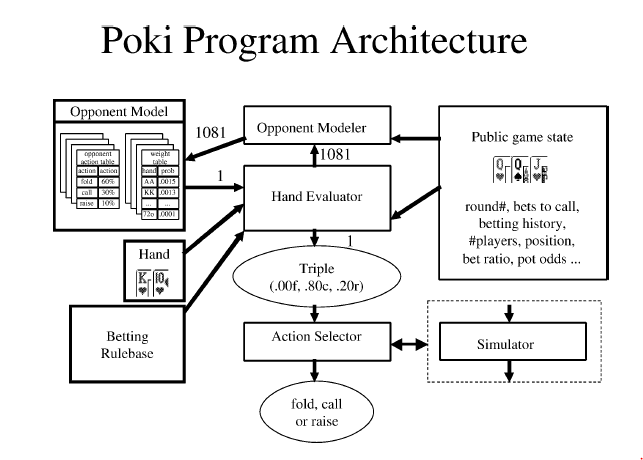
\includegraphics[width=0.9\textwidth]{figuras/Poki.png}   
\caption{Arquitectura de Poki \cite{Billings}}
\label{fig:poki}
\end{figure}

En el preflop, \textit{Poki} modela a cada oponente como una distribución de probabilidades según la mano que puedan tener, modelado que se genera con una estrategia de apuestas basadas en reglas y obtiene parámetros de cada uno de los oponentes en función de las acciones de cada jugador. Tras el flop, \textit{Poki} evalua el valor de la mano en el contexto de la ronda (considerando cada uno de los oponentes y su modelado, así como las apuestas y las cartas, entre otros factores), usando una  apuesta basadas en reglas más complejas que en el preflop y generando las posibles acciones que pueda tener el programa en ese contexto, además de utilizar un simulador que itera este proceso teniendo en cuenta diferentes posibles manos de los oponentes. Este proceso cíclico se repite cada vez que sea necesario actuar por parte de \textit{Poki}.

La abstracción en este software se centra en el procesado de datos, pues las acciones las procesa usando una probabilidad triple. Esto se refiere a que cada modelado, incluido el del propio \textit{Poki}, se basa en un conjunto ordenado de tres valores: PT = \{f,c,r\}. Cada uno de estos valores representa la distribución de probabilidades de que la próxima acción de ese jugador sea pasar, ver o subir la apuesta, respectivamente.\cite{Billings}

Esta abstracción permite gran parte de los elementos problemáticos de una partida de póker (tales como la fuerza o el potencial de una mano) en un único elemento (siendo una abstracción de información). 

Si bien este software ha ido mejorando con el paso del tiempo, pudiendo vencer a jugadores de cada vez mayor nivel, este software no es capaz de enfrentarse adecuadamente a un jugador profesional. Por otro lado, es uno de los pocos softwares que simulan partidas de múltiples jugadores (ya que una de las abstracciones más habituales que hacen los programas de póker es centrarse en la modalidad heads-up, o modalidad de dos jugadores, ya que elimina tanto el modelado de múltiples oponentes cómo el factor de la posición con respecto al dealer, que en una partida real tiene una importancia relevante).

\subsection{\textit{Libratus}}

\textit{Libratus} \cite{libratusScience2, libratusScience} es un software de inteligencia artificial diseñado para jugar partidas de Póker sin límite de apuestas de dos jugadores (Heads-Up No-Limit poker o HUNL poker) desarrollado por Noam Brown and Tuomas Sandholm, miembros del departamento de Ciencias de Computación de la universidad Carnagie Mellon
Cómo se ha mencionado al final del apartado anterior, el optar por esta modalidad elimina la complejidad computacional de múltiples oponentes y el posicionamiento. Además de eso, también evita escenarios donde las malas decisiones de uno de los jugadores convierta a un jugador en ganador, aunque la estrategia de dicho jugador no sea tan buena como la de otros.

El funcionamiento de \textit{Libratus} consiste en tres módulos de funcionamiento:
\begin{enumerate}
\item  \textbf{Módulo de Plano de estrategias.} Este módulo genera una abstracción del estado de juego, llamada plano de estrategias, mucho más pequeña y simple de resolver en la que se incluyen estrategias basadas en teoría de juegos que sirven de guía a la hora de jugar las rondas: siendo bastante detalladas para las primeras rondas y una aproximación para las rondas posteriores.
\item \textbf{Módulo de Solución de Subjuegos anidados.} Una vez que se alcanzan rondas mas avanzadas de la partida, este módulo genera una nueva abstracción más pequeña y precisa dentro de la primera abstracción y la resuelve en tiempo real, considerando esta solución siempre como parte de la estrategia incluida en el plano de estrategias para la partida entera. Si se da el caso de que el oponente realice una acción que no se contempla en esta segunda abstracción, se resuelve un subjuego que si incluye esa acción. A esto es lo que denominan resolución de subjuegos anidados.
\item \textbf{Módulo de Mejora.} Este módulo sirve para mejorar el plano de estrategias, pues completa los subjuegos faltantes de la abstracción del plano de estrategias, computando estrategias para cada uno de estos subjuegos faltantes. Además de eso, y a modo de optimización, prioriza unos u otros subjuegos en función de las acciones del oponente, ya que el intentar computar cada uno de los subjuegos restantes generaría un arbol tan grande para que esto pueda llegar a ser completado sin perder optimización del programa.
\end{enumerate}

\begin{figure}[h]
\centering

\includegraphics[width=0.9\textwidth]{figuras/Libratus.png}   
\caption{Visualización del funcionamiento de la abstracción de Libratus \cite{libratusScience2} y de la resolución de subjuegos anidados. Partiendo del plano de estrategias (triangulo superior), se generan varias abstracciones con sus propias estrategias (los triángulos en la base del plano de estrategias), siendo el triangulo más grande la que corresponde a la abstracción precisa generada analizando las acciónes (el camino blanco) que el oponente ha ido tomando, lo cual genera otros subjuegos anidados.}
\label{fig:libratus}
\end{figure}

Este software se probó tanto contra otros softwares de HUNL poker, entre ellosBaby Tartarian8\footnote{El Bot Baby Tartarian8 es un bot de inteligencia artificial para póker desarrollado también por Noam Brown y Tuomas Sandholm, que había derrotado al resto de inteligencias artificiales participantes en la Competición Anual de Poker por Ordenador (Annual Computer Poker Competition o ACPC) en el año anterior al desarrollo de Libratus con un margen de 12 ± 10 y 24 ±20 mili-ciega grande (mbb) por partida a los softwares más fuertes de dicho ACPC.} , así como algunos de mejores profesionales de HUNL Poker, resultando ganador \textit{Libratus} en ambos casos. \cite{libratusScience2, libratusScience}



\chapter{Fundamentos teóricos de juegos y póker}

\section{Gestión de la información en los juegos: Juegos de Información perfecta y Juegos de información Imperfecta}
\label{sec:info}

En apartados anteriores ya se ha mencionado los conceptos de información perfecta e información imperfecta relacionados con la teoría de juegos.\cite{Gametheory}
 Este concepto se utiliza como una forma de clasificar los juegos extensivos.

Se define como juego extensivo a la descripción explícita de la estructura secuencial de la decisión de los problemas encontrados por los jugadores en una situación estratégica, permitiendo a cada uno de los jugadores considerar su estrategia y acciones a tomar no solamente al comienzo de la partida, sino que también permite considerar su plan de acción en cualquier momento en el que tenga que hacer una decisión. \cite{Gametheory}

Habiendo definido lo que es un juego extensivo, se puede hacer la clasificación según la información. 

Se considera que un juego tiene información perfecta cuando, a la hora de tomar una decisión dentro de una partida, el jugador tiene información de todos los eventos que han ocurrido previamente y conoce al completo el estado de juego actual. Un juego extensivo con información perfecta tiene los siguientes elementos:

\begin{itemize}
\item Un conjunto $N$, que corresponde al conjunto de jugadores.
\item Un conjunto $H$, que es el conjunto de historias, donde cada uno de los componentes de la historia es una acción tomada por un jugador. Este conjunto $H$ de secuencias (finitas o infinitas) debe cumplir las siguientes condiciones:
\begin{itemize}
\item La secuencia vacía $\emptyset$ pertenece a $H$. Esta historia es el punto inicial de la partida, llamado habitualmente \textit{historia inicial}.
\item Si $(a^k)_{k=1,...,K}\in H$, donde $K$ puede ser infinito, y siendo $L< K$, entonces $(a^k)_{k=1,...,L}\in H$.
\item Si una secuencia infinita $(a^k)^\infty_{k=1}$ cumple que $(a^k)_{k=1,...,L}\in H$ para cada valor positivo entero $L$, entonces  $(a^k)^\infty_{k=1}\in H$.
   \end{itemize}
\item La función jugador $P$, que asigna a cada historia que no sea terminal (es decir, a cada miembro de$ H\backslash  Z$) un miembro de $N$. siendo $P(h)$ el jugador que tiene que tomar una decisión tras la historia $h$.
\item Un conjunto $Z$, que incluye todas las historias terminales. Una historia $(a^k)_{k=1,...,K}\in H$ es terminal si es infinita o si no hay ningún $a^{K+1}$ que cumpla  $(a^k)_{k=1,...,K+1}\in H$.
\item La relación de preferencia del jugador $i$. Es decir, para cada jugador $i \in N$, una relación de preferencia $\succsim_i$ sobre $Z$.
\end{itemize} 

Si el conjunto $\langle N,H,P\rangle$    cumple las tres primeras condiciones de la definición, se denomina forma de juego extensivo con información perfecta. \cite{Gametheory}

Algunos ejemplos de juegos de información completa son el ajedrez, el Go, las damas o el tres en raya.

Es necesario distinguir información perfecta de información completa. La información completa implica el conocimiento común de las estrategias, tipos de jugador y jugadas futuras de cada uno de los jugadores. Un juego de información perfecta puede tener o no información completa.

Se considera que un juego tiene información imperfecta cuando, en el momento en que tenga que tomar una acción un jugador, ese jugador solo tiene información parcial sobre las acciones tomadas previamente y/o del estado actual del juego. Un juevo extensivo con información imperfecta tiene los siguientes elementos:
\begin{itemize}
\item Un conjunto $N$, que corresponde al conjunto de jugadores.
\item Un conjunto $H$, que es el conjunto de historias, donde cada uno de los componentes de la historia es una acción tomada por un jugador. Este conjunto $H$ de secuencias (finitas o infinitas) debe cumplir las siguientes condiciones:
\begin{itemize}
\item La secuencia vacía  $\emptyset$ pertenece a $H$. Esta historia es el punto inicial de la partida, llamado habitualmente \textit{historia inicial}.
\item Si $(a^k)_{k=1,...,K}\in H$, donde $K$ puede ser infinito, y siendo $L< K$, entonces $(a^k)_{k=1,...,L}\in H$.
\item Si una secuencia infinita $(a^k)^\infty_{k=1}$ cumple que $(a^k)_{k=1,...,L}\in H$ para cada valor positivo entero $L$, entonces  $(a^k)^\infty_{k=1}\in H$.
   \end{itemize}
\item La función jugador $P$, que asigna a cada historia que no sea terminal (es decir, a cada miembro de $ H\backslash  Z$) un miembro de N$ \cup \{c\}$. siendo $P(h)$ el jugador que tiene que tomar una decisión tras la historia $h$. Si$ P(h) = c$  entonces es la probabilida la que determina la acción tras la historia $h$.
\item Un conjunto $Z$, que incluye todas las historias terminales. Una historia $(a^k)_{k=1,...,K}\in H$ es terminal si es infinita o si no hay ningún $a^{K+1}$ que cumpla  $(a^k)_{k=1,...,K+1}\in H$.
\item El conjunto $A$ que incluye las acciones disponibles tras una historia no terminal h. $A(h)=\{a:(h,a) \in H \}$.
\item Una función $f_c$ que asocia a cada historia $h$ que que sea $ P(h) = c$ una medida de probabilidad $f_c(\cdot|h)$ en $A(h)$, donde cada una de las medidas de probabilidad es independiente de las demas medidas, siendo $f_c(a|h)$ la probabilidad de que a ocurra tras $h$.
\item Para cada jugador $ i \in N$ una partición de información $\mathcal{I}_i$ de $\{ h \in H:P(h) = i \} $ cumpliéndose que $A(h) = A(h')$ siendo $h$ y $h'$ miembros de la misma partición. Se denomina conjunto de información del jugador $i$ al conjunto $I_i \in \mathcal{I}_i$.  Para cada $I_i \in \mathcal{I}_i$ se llama $A(I_i)$ al conjunto $A(h)$ y $P(I_i)$ al conjunto $P(h)$
\item La relación de preferencia del jugador $i$. Es decir, para cada jugador $i \in N$, una relación de preferencia $\succsim_i$ en riesgo sobre $Z$, que puede ser representado como el valor esperado del resultado de una función definida en $Z$.
\end{itemize} 

Si el conjunto $\langle N,H,P, f_c,(\mathcal{I}_i)_{i \in N}\rangle$ cumple estas condiciones, se denomina forma de juego extensivo de información inperfecta. \cite{Gametheory}

El grado de información de la que dispone cada jugador viene dado por $\mathcal{I}_i$. Estas particiones de cada jugador son un principio de la partida, ya que cada jugador puede  distinguir entre diferentes historias de su partición sin necesidad de hacer cualquier inferencia sobre las acciones de los demás jugadores. A medida que la partida se desarrolle, un jugador puede ser capaz de hacer inferencias que precise la información que disponga, en función de las acciónes de los demás jugadores.\cite{Gametheory}

Los juegos de cartas donde cada jugador tenga cartas privadas (es decir, que sean cartas que los demás jugadores no conocen), tales como el póker, el mus, el bridge o el blackjack, son ejemplos de juegos de información imperfecta. En estos se combina la información pública (información conocida por todos los jugadores) como información privada (información conocida únicamente por el jugador), creando en ellos interés para ser considerados desde el punto de vista de la inteligencia artificial. En el siguiente apartado se hablará de estos juegos con un poco más de profundidad.

\section{Juegos de Cartas}
\label{sec:cartas}

Dado el interés que despertan los juegos de información imperfecta desde el punto de vista de la inteligencia artificial, se van a explicar las bases de algunos de estos juegos. En concreto, de los juegos de cartas mencionados en el apartado anterior. Estos juegos comparten que son juegos de cartas con apuestas, pero cada uno con sus propias reglas y peculiaridades.

\subsection{Póker}

El póker engloba a un conjunto de juegos de cartas con apuestas, que comparten similitudes en las reglas y, en concreto, comparten la forma de apostar. El póker se juega habitualmente usando la baraja francesa estándar\footnote{Barajas de 52 cartas agrupadas en cuatro palos de 13 cartas cada uno: Tréboles, Picas, Diamantes y Corazones. Las 13 cartas que componen cada palo son As, 2 al 10 y 3 figuras: Jota (J), Reina (Q) y Rey (K).}, aunque en algunas variaciones se utilizan también los comodines de las barajas (dando lugar a barajas de 54 cartas). 

Las diferentes variaciones de póker tienen un funcionamiento similiar. En cada ronda de una partida de póker, uno o varios jugadores tienen que hacer una apuesta inicial obligatoria llamada \textit{ciega} (en inglés, \textit{blind}), tras lo cual se reparten cartas a cada jugado. Se desarrolla la ronda de juego mediante rondas de apuestas, donde cada jugador puede tomar una de las acciones establecidas en el orden establecido en sentido horario desde el jugador inicial. El jugador a la derecha del jugador inicial de cada mano recibe el nombre de \textit{dealer}, que es el jugador que actúa el último en cada ronda de apuestas. El \textit{dealer} también se encarga de barajar y repartir las cartas en caso de que no haya una persona encargada de hacerlo.\cite{howto}
Las posibles acciones de apuesta son:
\begin{itemize}
\item \textit{Ver} la apuesta, que iguala la apuesta de ese jugador a la apuesta más alta de la mesa.
\begin{itemize}
\item En el caso de que no haya una apuesta por encima de las demás sin que se haya producido ninguna acción de \textit{ver}, \textit{ver} la apuesta significa no tomar acción hasta que haya una variación de apuestas. En esa situación, si todos los jugadores \textit{ven} la apuesta sin que se haya producido una variación de apuestas en esa ronda de apuestas, la ronda de apuestas se da por finalizada.
\end{itemize}
\item \textit{Subir} la apuesta (aumentando su apuesta hasta una cantidad a su elección siempre que supere a la apuesta más alta de la mesa).
\item \textit{Pasar} la apuesta. Si un jugador decide \textit{pasar} la apuesta, significa que se retira de esa ronda de juego y no puede apostar más hasta la siguiente ronda de juego. 
\end{itemize}

Una ronda de apuestas acaba cuando todos los jugadores han \textit{visto} la apuesta más alta o cuando sólo uno de los jugadores no ha \textit{pasado} durante la ronda de juego actual. En el primer caso, las apuestas se suman al bote de la ronda de juego, y se continua con dicha ronda de juego. En el segundo caso, el jugador que no ha \textit{pasado} sería el ganador de la ronda de juego.

Entre cada una de las rondas de apuestas, los jugadores desarrollan su jugada con las cartas disponibles, dependiendo de la modalidad.
Cuando acaban todas las rondas de apuestas de una ronda de juego, si quedan al menos 2 jugadores sin que hayan \textit{pasado}, se revelan las cartas y se comparan las jugadas construidas por estos jugadores y determinando el ganador de la ronda de juego.

El ganador de la ronda de juego se queda con todo el dinero del bote de esa ronda de juego.

El póker tiene muchas variaciones, pero las más habituales son las siguientes\cite{pokertypes, howto} :

\begin{itemize}
\item \textbf{Five-Cards Draw.} También conocido como \textbf{Cantrell Draw}. En cada ronda de juego de esta variante se reparten 5 cartas a cada jugador que, tras la primera ronda de apuestas, se podrán cambiar tantas cartas como se quieran de dicha mano (desde ninguna hasta las 5 cartas), llevando a una segunda y última ronda de apuestas. El Five Cards Draw es la variante considerada más sencilla de todas, que permite familiarizarse con el juego y aprender el funcionamiento del póker.
\item \textbf{Texas Hold'em.} La principal característica de esta modalidad de Póker es el reparto de cartas. Mientras que en el Five-Cards Draw se reparten cinco cartas ocultas a cada jugador, en el Texas Hold’em se reparten dos cartas ocultas a cada jugador y se revelan a todos los jugadores un total de cinco cartas a lo largo de las fases de juego, dejando la posibilidad a cada jugador de formar su mejor jugada de cinco cartas entre el total de siete cartas disponibles para cada jugador. Esta variante es conocida como una de las más populares de póker.
\item \textbf{Omaha Hold'em.} Conocido habitualmente como \textbf{Omaha}. Esta modalidad de póker es muy similar a Texas Hold'em, aunque con dos variaciones principales: cada jugador recibe 4 cartas ocultas en lugar de dos y la jugada de 5 cartas formada tiene que estar formada siempre por 3 de las 5 cartas comunes y por 2 de las 4 cartas de la mano. El resto del desarrollo de cada ronda de juego es prácticamente idéntico al de Texas Hold'em (como modificaciones en función de cada una de las submodallidades de Omaha).
\item \textbf{Seven-card Stud.} En esta modalidad, cada jugador recibe inicialmente 2 cartas ocultas y una visible, carta con la que se determina el jugador inicial. A medida que se desarrolla la ronda de juego, cada jugador va recibiendo cartas visibles y ocultas tras cada una de las rondas de apuestas, acabando con una mano de 7 cartas (3 ocultas y 4 visibles), con la que tiene que formar la mejor jugada posible de 5 cartas. El desarrollo se puede resumir en \textit{2 ocultas, 4 visibles y 1 oculta}, ya que es el orden en que se reciben las cartas que forman su mano.
\end{itemize}

\subsection{Mus}

El Mus es un juego de cartas con apuestas que se suele jugar entre 4 jugadores (agrupados en dos parejas), jugándose con una baraja española estándar\footnote{Barajas de 40 cartas agrupadas en cuatro palos de 10 cartas cada uno: Oros, Copas, Espadas y Bastos. Las 10 cartas que componen cada palo son As(1), 2 al 7 y 3 figuras: Sota (10), Caballo (11) y Rey (12).}. Al ser habitual el jugarse por parejas, cada uno de los miembros se posiciona en la mesa enfrente del otro, de manera que nunca puedan tener acción dos jugadores de la misma pareja.

\begin{figure}[h]
\centering
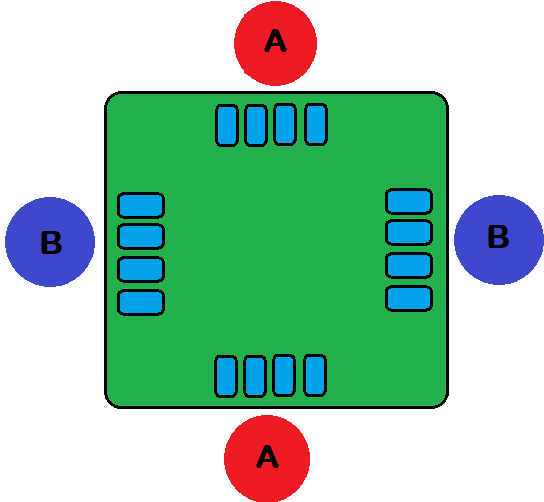
\includegraphics[width=0.75\textwidth]{figuras/Mus.png}   
\caption{Esquema de la distribución de los jugadores en una partida de Mus. \cite{propiaPaint}}
\label{fig:mus}
\end{figure}

La puntuación de cada carta (valor en torno al que gira todas las apuestas) varía según las variaciones de reglamento. Principalmente se consideran 2 versiones del reglamento. \cite{mus,mus2}
\begin{itemize}
\item \textbf{4 Reyes y 4 Ases.} Reglamento habitual en el Pais Vasco. Las cartas del As al 7 valen tantos puntos como número impreso en la carta (1-7) mientras que las figuras valen 10 puntos.
\item \textbf{8 Reyes y 8 Ases} Reglamento habitual en el resto de España. En este caso, los treses son equivalentes a los reyes (valiendo 10 puntos) y los doses son equivalentes a los ases (valiendo 1 punto). Al ser equivalentes, un tres y un Rey juntos forman una pareja, lo mismo que un As y un 2. El resto de valores es idéntico a la modalildad de 4 Reyes y 4 Ases.
\end{itemize}

Las figuras solo tienen el mismo valor para el lance de Juego/Punto, para el resto de lances tienen un orden de valor: Rey/Tres (en caso de 8 reyes)$>$Caballo$>$Sota.

Durante cada ronda de juego, llamadas \textit{manos}, se reparten 4 cartas a cada jugador, ocultas para los demás jugadores. Empezando por el jugador inicial, que también recibe el nombre de \textit{mano}, cada jugador decide si \textit{pide Mus}, es decir, diciendo si quiere cambiar alguna carta de su mano o si no quiere cambiar cartas de su mano (diciendo \textit{Mus} en caso de que quiera cambiar o  \textit{No hay mus} en caso de que no quiera). Si todos los jugadores piden Mus, empezando por el jugador que es mano descarta tantas cartas como quieran de su mano (siempre descartando, al menos, una carta) y recibiendo tantas cartas como haya descartado y se vuelve a preguntar a los jugadores si quieren Mus. En el momento en que un jugador no quiera Mus, comienzan las apuestas. \cite{mus}

Las apuestas, llamados \textit{envites}, durante cada una de las manos de Mus se dividen en 4 categorías, llamadas \textit{lances}. Los \textit{lances} de una partida de Mus son los siguientes (numerados por el orden en el que se realizan en cada ronda):
\begin{enumerate}
\item \textbf{Grande.} Cuanto mayor sea el valor de la combinación, mejor es la combinación para este lance. 
\item \textbf{Chica.} Cuanto menor sea el valor de la combinación, mejor es la combinación para este lance.
\item \textbf{Pares.} Cuantas más cartas del mismo valor y mayor sea ese valor, mejor es la combinación. Este lance solo se apostará si al menos un jugador de cada pareja tiene Pares.
\item \textbf{Juego /Punto.} En el lance de Juego, el objetivo es alcanzar 31 (siendo la mejor combinación para Juego) o superar 31 (cuanto mayor sea el valor en este caso, mejor). En caso de que ningún jugador supere los 31 puntos con las cartas que tienen, se apuesta por el lance de Punto. Para el lance de Punto, cuanto más se acerce el valor a 30, mejor es la combinación.
\end{enumerate}

Tras realizar los envites de todos los lances, se revelan las cartas y se determina qué pareja gana cada lance en el que se haya apostado, sumando los puntos apostados. Cuando una de las parejas alcance un número de puntos preacordado al comienzo de la partida (por lo general 30 ó 40 puntos), se acabará la partida, ganando esa partida la pareja con más puntuación.

A pesar de que cada jugador tenga sus 4 cartas y sean ocultas, si uno de los jugadores de la pareja gana un lance, la pareja como tal gana (ya que la puntuación de la partida se cuenta por pareja, no por jugador), lo cual fuerza a jugar con las cartas del compañero, pero manteniendo tus cartas ocultas para los oponentes. Para ello, es importante el uso de señas entre los miembros de una pareja para intentar comunicarse las jugadas que tienes.

\subsection{Bridge}

El Bridge\cite{bridge} es un juego de cartas de apuestas para 4 jugadpres que se juega con una baraja francesa estándar. Es juego se juega por parejas,  por lo que cada uno de los jugadores de la pareja se sienta enfrente de una manera equivalente a la vista en la figura \ref{fig:mus}. 

Lo más característico del Bridge es que la apuesta se hace es cuántas manos de una misma ronda puede ganar la pareja. Esta apuesta consiste en un número y un palo. El número indica cuantas manos por encima de 6 se pueden ganar, siendo el palo de triunfo el palo de la apuesta. En el caso de que se  haga una apuesta sin Triunfo, ningún palo será palo de triunfo. \cite{bridge}

El Bridge consiste de dos fases principales: el \textit{remate} y el \textit{carteo}.

Durante una partida de Bridge, uno de los jugadores baraja y reparte entre todos los jugadores todas las cartas del mazo, lo que da la comienzo al \textit{remate}. Esta ronda es la ronda de apuestas, en la que se tienen que apostar cuántas manos por encima de 6   El jugador que reparte se convierte en el primer subastador, que recibe el nombre de \textit{dador}. El dador puede hacer la apuesta o pasar al jugador de su izquierda.  \cite{bridge}

En el momento en que un jugador hace una apuesta, los demás jugadores pueden tomar una de las siguientes acciones:
\begin{itemize}
\item \textit{Ver} la apuesta.
\item \textit{Doblar} la apuesta, en el cual se sube al menos uno de los elementos de la apuesta (número o palo) hecha por la pareja oponente. En el caso de que el oponente haya doblado la apuesta, se considera que se \textit{redobla} la apuesta.
\item \textit{Pasar} la apuesta. 
\end{itemize} 

El número de la apuesta puede ir desde 1 (que significa que el apostante ganaría, al menos, 7 manos) hasta 7 (Que significa que el apostante ganaría las 13 manos).
La posibilidad de doblar el palo de la apuesta, hace que sea necesario establecer un orden de los palos.  El orden establecido es (de mayor a menor): Sin Triunfo, Picas, Corazones, Diamantes y Tréboles. 

A la hora de doblar es necesario quela nueva apuesta sea superior Una apuesta doblada puede mantener el mismo número pero aumentando el palo, al igual que si se aumenta el número de la apuesta, se puede poner cualquier palo como palo de triunfo. Es decir, que si la apuesta es  \textit{3 Diamantes}, se puede doblar la apuesta con  \textit{3 Picas}, al igual que con cualquier apuesta con un numero mayor a \textit{3}. Además, la única forma de doblar una apuesta con palo \textit{Sin Palo} es usando una apuesta de mayor número.\cite{bridge}

Cuando todos los jugadores han visto una apuesta, esta apuesta se la denomina como \textit{contrato}, y se asignan los papeles para la ronda del \textit{carteo}:
\begin{itemize}
\item El jugador que hizo el contrato se convierte en el  \textit{Declarante}.
\item La pareja del declarante se convierte en el \textit{Muerto}.
\item Los otros dos jugadores se convierten en los \textit{defensores}.
\end{itemize} 

En este momento comienza el \textit{carteo}. En esta fase es en la que se juegan las 13 manos de la ronda, en la cual el declarante tiene que ganar tantas manos como dice el contrato, mientras que los defensores intentarán evitarlo. 
La primera mano de esta fase la inicia el defensor sentado a la izquierda del declarante, que jugará una carta de su mano. Tras eso, el muerto muestra sus 13 cartas, colocándolas en el centro de la mesa ordenadas por palo y número. Estas cartas las jugará el declarante en cada una de las manos de esta ronda (por lo que el muerto no jugará el resto de la ronda). Una vez reveladas y ordenadas todas las cartas, el resto de jugadores tienen que jugar una carta del mismo palo que la carta inicial. En caso de no tener cartas del mismo palo, se puede jugar una carta de cualquier palo. \cite{bridge}

El ganador de la mano es el jugador que haya jugado la carta del palo inicial con el número más alto. La excepción a esto es el caso en que, al menos, un jugador haya jugado una carta del palo de triunfo (si lo hay). En esta situación, gana la mano el jugador que haya jugado la carta del palo de triunfo (en caso de que más de un jugador haya jugado una carta de ese palo, gana el jugador con la carta de triunfo de valor más alto).

El resto de las manos siguen este orden:

\begin{center}
 Defensor 1 $\rightarrow$ Declarante (usando las cartas del Muerto) $\rightarrow$ Defensor 2 $\rightarrow$ Declarante (con sus cartas).
\end{center}

Al final de la ronda, se cuentan las manos ganadas en una ronda. Si el declarante ha ganado las manos que apostó en el contrato, la pareja ganará tantos puntos según el número de la apuesta y el palo de triunfo de la misma.\cite{bridge}

\subsection{Blackjack}

El Blackjack \cite{blackjack} es un juego de apuestas que se usan barajas francesas estándar. Se puede jugar con una única baraja, pero lo habitual es mezclar barajas (siendo el más popular el de 6 barajas). 

En el Blackjack, el objetivo de los jugadores es conseguir sumar 21 puntos con las cartas de su mano, o quedarse lo más cerca posible sin pasarse. Así mismo, tienen que intentar superar a la jugada del crupier para ganar. Para esto, se suma el valor de las cartas de cada jugador. El valor de las cartas es el siguiente:
\begin{itemize}
\item 2-10: El valor de la carta
\item J,Q,K: 10 Puntos
\item A: 11 ó 1 Punto. Vale 11 puntos si la suma total no supera 21 o 1 en caso de que los supere.
\end{itemize} 

En el caso de que un jugador consiga una puntuación de 21 puntos con todas las cartas de su mano, se considera que ese jugador ha conseguido Blackjack.

En cada partida, se define un valor de apuesta fijo, que se mantiene salvo que se anuncie la subida de la apuesta. 
Al comienzo de la ronda, cada jugador coloca la apuesta fija delante suya y, despues de eso, el crupier reparte a cada jugador una carta bocarriba, y se reparte una carta a si mísmo bocarriba tambien. Tras eso, repite el proceso, con la salvedad de que la segunda carta del crupier suele ser oculta (dependiendo de las normas de la partida). Si la segunda carta del crupier es oculta, también lo es para el propio crupier.

Tras esto, es necesario comprobar si alguno de los jugadores tiene 21 natural, es decir,si su mano inicial incluye un As y una de las cartas de 10 puntos. En caso de que un jugador tenga un Blackjack natural, gana las fichas de los demas jugadores. En caso de que más de un jugador (crupier incluido) consiga Blackjack natural, se produce un empate, en la cual los jugadores con 21 recuperan su apuesta, y el resto de jugadores pierden lo apostado.

En la única situación en la que el crupier puede ver su carta antes de su turno es para comprobar si tiene un Blackjack Natural, es decir, solamente en caso de que su carta visible sea un As o una carta de 10 puntos.

Si ningún jugador tiene 21 natural, se comienza la ronda de apuestas. Empezando por el jugador más a la izquierda, cada jugador puede pedir una carta o plantarse. El jugador puede pedir cartas hasta que decida plantarse o hasta que se pase de 21. En el momento en que un jugador supere 21 puntos, pierde automáticamente, y el crupier toma la apuesta del perdedor. 

Cuando todos los jugadores hayan recibido cartas, es el turno del crupier de pedir cartas. Revela la carta bocabajo y toma la acción pertinente según la suma de sus cartas. Por lo general, está obligado a pedir carta mientras sume 16 o menos puntos, y a plantarse en cuanto sume 17 o más.

Una vez ha terminado el turno del crupier, se procede a hacer el recuento de los valores de los jugadores, en función del valor de la jugada del crupier y de los jugadores:
\begin{itemize}
\item Si el crupier se ha pasado de 21: Cada jugador recupera su apuesta y el crupier paga a cada jugador su apuesta.
\item Si el crupier tiene menos de 21 y ningún jugador ha conseguido Blackjack: Los jugadores que tengan menos puntuación que el crupier pierden su apuesta, y los jugadores que tengan más puntuación que el crupier recuperan su apuesta y el crupier les paga su apuesta.
\item Si el crupier y un jugador empatan: Ningún jugador pierde sus fichas ni recibe fichas.
\end{itemize} 

\begin{figure}[tb]
\centering
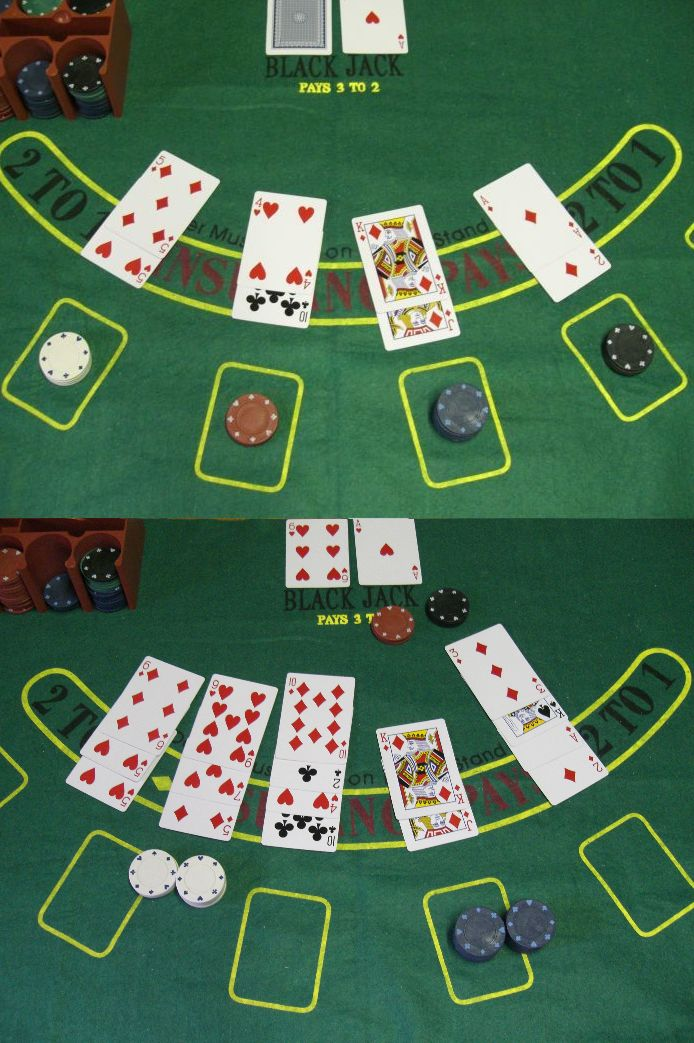
\includegraphics[width=0.5\textwidth]{figuras/blackjack.jpg}   
\caption{Ejemplo de una partida de Blackjack. En la imagen superior, se encuentra cómo es la partida antes de empezar el turno de los jugadores. En la imagen inferior, el resultado de la partida tras acabar la acción del Crupier.\cite{mesa}}
\label{fig:black}
\end{figure}


Además de pedir cartas o plantarse, los jugadores pueden tomar 3 opciones adicionales, pero estas opciones están limitadas a condiciones:
\begin{itemize}
\item \textbf{Separar:}Esta opción solo está disponible si las dos cartas iniciales del jugador son pareja. Separar permite al jugador dividir las cartas de su mano en dos apuestas al comienzo de su turno, siendo necesario apostar para la segunda mano. Por lo que queda de mano, cada una de las apuestas son tratadas como si fueran independientes.
\item \textbf{Doblar:} Esa acción permite al jugador pedir una única carta bocabajo, que se mantiene bocabajo hasta el final de la mano. Por lo general, solo se puede pedir esta acción si las cartas iniciales de ese jugador 9, 10 ó 11. 
\item \textbf{Asegurar:}Si la carta revelada del crupier es un As, los jugadores pueden apostar a Asegurar. Esto hace que el jugador apueste la mitad de su apuesta actual en el Seguro. En caso de que el crupier obtenga un Blackjack, la apuesta principal la sigue perdiendo, pero el jugador que haya apostado a Asegurar gana el doble de lo apostado en el Seguro.
\end{itemize} 

Por último, uno de los elementos mas importantes es el conteo de las cartas que han salido a lo largo de la partida, pues el mazo no se baraja al final de cada mano, sino que se baraja únicamente cuando se acaba el mazo. También baraja el mazo cuando acaba la ronda de juego.\cite{blackjack}

\section{Criterios para la elección de un juego de cartas}
\label{sec:choices}

Una vez expuestos algunos ejemplos que pueden ser sujeto de estudio, es necesario tomar la decisión de cuál centrarse en el proyecto. Para ello, se establecen los siguientes criterios a la hora de hacer la elección:
\begin{itemize}
\item Gestión de la información: Debido al interés que suscita desde el punto de vista de la inteligencia artificial, se busca un juego de información imperfecta. Además, que pueda manejar de manera eficiente y uniforme la información pública.
\item Complejidad del arbol de decisiones: Un arbol de decisiones complejo es consecuencia de un alto nivel de combinatoria de acciones, pues se generan muchos posibles estados en función de los estados de juego. Esta complejidad obliga a que la inteligencia artificial tenga que ser adaptable, siendo un punto de interés para su estudio. 
\item Individualización de la toma de decisiones: Una de los primeros factores que se quieren eliminar para poder desarrollar el estudio del juego es el factor externo de la colaboración. En otras palabras, se quiere eliminar la posibilidad de que la toma de decisiones dependa de la información de un jugador que no sea el oponente.
\item Dificultad de juego: Este critero sirve para medir como de complicado son las normas del juego. Un juego con reglas sencillas, fácil de aprender, pero complejo a la hora de dominarlo es el juego que mejor cumple este criterio.
\end{itemize} 

En base a estos criterios, se examinan los juegos susceptibles de análisis, es decir, los mencionados previamente en este proyecto:

\begin{itemize}
\item Go y ajedrez: a pesar de ser juegos con una altísima complejidad del arbol de decisiones(del orden de $10^{360}$ y del orden de $10^{123}$), al ser un juego de información perfecta, queda descartado.
\item Póker: El póker es un juego de información imperfecta, con una complejidad de arbol de decisiones bastante alta (variando según la modalidad), la toma de decisiones es individual y las reglas básicas comunes son sencillas. El póker si cumple los cuatro criterios.
\item Bridge: Este juego es un juego estrictamente por parejas, por lo que no cumple el criterio de individualización.
\item Mus: Si bien es cierto que este juego tiene modalidad de jugadores individuales, el juego más extendido es el juego por parejas, por lo que no cumpliría el criterio de individualización.Además de eso, el grado de complejidad del arbol de decisiones es bastante inferior al de los demás juegos mencionados aqui, por lo que tampoco cumpliría el de complejidad.
\item Blackjack: El Blackjack es un juego sencillo cuyas decisiones se toman de manera individual. El problema viene con la información y la complejidad. Si bien es un juego de información imperfecta, si se mantiene el mismo estado inicial que para otros juegos como póker (es decir, 2 jugadores con un solo mazo), disminuye drásticamente la complejidad del arbol de decisiones de este juego. Además, siguiendo el flujo de juego normal del Blackjack, el flujo de información no es uniforme, pues está ligado completamente a las acciones, incluso dando lugar a estados que son callejones sin salida. Por estos motivos no cumple estos dos criterios.
\end{itemize} 

De esta manera, el único juego que cumple los cuatro criterios es el póker, lo que lo convierte en el juego elegido.
A continuación se detalla cuál de las variaciones de póker es el juego elegido para ser objeto de estudio de este proyecto. Es necesario considerar algún criterio adicional  a los arriba mencionados, pues la individualización de la toma de decisiones no varía en las modalidades estudiadas, mientras que la dificultad de juego apenas varía entre las modalidades.
Los criterios  a considerar para discernir cuál es la variación de póker a elegir son los siguientes:
\begin{itemize}
\item Gestión de la información: Este criterio evalúa en este momento la cantidad de información pública y privada que presenta cada uno de los juegos. La cantidad de información pública es muy importante de cara a desarrollar una inteligencia artificial, pues permite definir con más precisión el estado de juego actual y ayuda a establecer una estrategia adecuada.
\item Complejidad del arbol de decisiones: Este criterio evalúa la cantidad de estados de juego y de toma de decisiones que posee el juego.
\item Adaptabilidad y versatilidad: Con este criterio se busca evaluar cómo de versátil es el flujo de juego para permitir a los jugadores una corrección de estrategia en función de la información conocida.
\item Limitaciones de juego: Con este criterio se quiere evaluar si existe alguna limitación a la hora de tomar decisiones, establecer estados o que se den callejones sin salida.
\end{itemize}

Con estos criterios, se procede a evaluar las cuatro variantes de póker mencionadas en este proyecto:
\begin{itemize}
\item Five-Cards Draw. El Five-Cards Draw no cumple  el criterio de la adaptabilidad (puesto que solo se dispone de una actualización de información, limitando las acciones de los jugadores. Además de eso, es el único de los cuatro que no tiene cartas como información pública, siendo la información conocida la apuesta del oponente y el número de cartas
\item Texas Hold'em. El Texas Hold'em cumple los 4 criterios. No tiene ninguna limitación adicional, tiene una gran cantidad de estados posibles ($5.56*10^{13}$)\footnotemark, es una de las dos versiones que más información pública tiene (5 cartas reveladas comunes), que se va incrementando durante la ronda, y un total de 4 rondas de apuestas donde poder corregir la estrategia en función de la información revelada.
\item Omaha Hold'em. Si bien el Omaha es el que tiene la mayor cantidad de estados posibles ($1.14 * 10^{18}$)\footnotemark[\value{footnote}] y tiene la misma información pública que el Texas Hold'em, la cantidad de información oculta es mayor (ya que es necesario considerar cada una de las cuatro cartas ocultas del otro jugador) y, además, se crea una limitación a la hora de formar la combinación de cartas (3 cartas de mesa y 2 de mano), lo cual hace que el criterio de Limitaciones de juego no se cumpla.
\item Seven-card Stud. El Seve-card Stud es el juego con mayor adaptabilidad y versatilidad de los 4, pues tiene 5 rondas de apuestas. Pero teniendo en cuenta que es más dificil modelar al oponente (ya que tiene menos información pública de cada oponente que el Omaha o el Texas Hold'em), y que tiene una limitación de juego, y es que la ordenación de jugadores no es secuencial entre rondas, pues el jugador inicial se decide por la carta más baja de las cartas reveladas), no cumple el criterio de Limitaciones de juego.
\end{itemize}

\footnotetext{El cálculo de estos estados posibles se ha realizado mediante una multiplicación de la combinatoria posible en cada uno de los juegos. Para Texas es $\binom{52}{2}*\binom{50}{2}*\binom{48}{3}*45*44 =5.56*10^{13}$, para Omaha es $\binom{52}{4}*\binom{48}{4}*\binom{44}{3}*43*42=1.14 * 10^{18}$ y para el Seven-card es $\binom{52}{7}*\binom{45}{7}=6.07*10^{15}$. El caso del Five-cards es particular, pues los estados varían en función de las cartas descartadas tras la primera ronda de apuestas, siendo el número de estados base $\binom{52}{5}*\binom{47}{5}=3.99*10^{12}$. }
El único que cumple simultáneamente los 4 criterios es el Texas Hold'em, lo que lo convierte en el juego elegido para este estudio.

\section{Fundamentos teóricos de póker Texas Hold'em}
\subsection{Desarrollo de las partidas: Apuestas y Fases de Juego}

En el Texas Hold'em\cite{howto} se reparte dos cartas a cada jugador como mano inicial, cartas ocultas para los demás jugadores, cartas que se van incrementando con las 5 cartas que se van revelando a lo largo de las rondas de apuestas posteriores a la inicial. Además de eso, al comienzo de cada una de las 3 rondas en las que se revelan cartas comunes, la carta superior del mazo es descartada. Esto se conoce como \textit{quemar} una carta\footnote{Este elemento se introdujo como un elemento de seguridad para evitar que en una partida real el crupier pueda favorecer a algún jugador, pero no tiene influencia alguna en la probabilidad. En el modelado se va a incluir únicamente por mantener el parecido con el juego real, pero es un elemento totalmente inócuo para el funcionamiento del simulador o del algoritmo.}. 

A pesar de que una partida de Texas hold’em podría tener hasta 22 jugadores iniciales (44 cartas repartidos a los jugadores, las 5 cartas reveladas y las 3 cartas quemadas), las partidas, tanto en casinos como en torneos, ocurren en mesas de 2 a 10 jugadores. Este límite está establecido con el fin de mantener el dinammismo de la partida, pues un aumento de jugadores ralentizaría el juego.

A lo largo de cada ronda, las cartas se van repartiendo y revelando a los jugadores, y tienen cuatro rondas de apuestas, en las que cada jugador debe tomar una de las acciones de apuestas posibles:
\begin{itemize}
\item \textbf{Ver} la apuesta. En inglés \textit{Call}, que iguala la apuesta de ese jugador a la apuesta más alta de la mesa.
\begin{itemize}
\item En el caso de que no haya una apuesta por encima de las demás sin que se haya producido ninguna acción de \textit{ver}, \textit{ver} la apuesta significa no tomar acción hasta que haya una variación de apuestas. En esa situación, si todos los jugadores \textit{ven} la apuesta sin que se haya producido una variación de apuestas en esa ronda de apuestas, la ronda de apuestas se da por finalizada. En este caso, la acción recibe el nombre de \textit{Check} en inglés.
\end{itemize}
\item \textbf{Subir} la apuesta. En inglés \textit{Raise}, esta acción permite aumentar la apuesta del jugador a una cantidad a su elección, siempre que la cantidad de la nueva apuesta sea superior a la apuesta más alta de la mesa.
\item \textbf{Pasar} la apuesta. En inglés \textit{Fold}, esta acción significa descartar la mano y retirarse de la ronda de juego. Esto implica que un jugador que \textit{pase} no puede apostar más hasta la siguiente ronda de juego. 
\end{itemize}

Cada jugador va realizando apuestas de manera secuencial hasta que todos los jugadores han visto la apuesta, o hasta que todos los jugadores pasan menos uno. En este caso, la ronda finaliza, y el jugador que no ha pasado recibe el total de lo apostado.\footnote{Los casinos suelen aplicar una comisión de un \% sobre el total de la apuesta. A esto se le conoce como \textit{rastrillo} o \textit{rake} en inglés. Debido a que es un elemento exclusivo de los casinos y no es un elemento del póker como tal, en el resto del proyecto no se va a tener en consideración ni se le hará mención.}  

Una vez explicado el funcionamiento de una ronda de apuestas, se procede a explicar las fases de cada ronda de juego.

Al comienzo de la ronda de juego, se entrega la posición de \textit{Dealer}\footnote{La traducción de Dealer es crupier y, en caso de que no haya una persona encargada del reparto, el crupier se hace cargo de repartir las cartas. Dado que el término crupier puede dar lugar a confusión, se mantendrá el término inglés a modo de nombre de la posición de este jugador} (representado por una ficha, conocida como \textit{button}) al jugador que le corresponde esa ronda. El \textit{button} se va rotando de jugador a jugador de manera secuencial: el jugador que ha sido jugador inicial en una ronda de juego, en la siguiente recibe el \textit{button} y el jugador a su izquierda se convierte en el jugador inicial de esa ronda.  El \textit{Dealer} es el jugador que está situado a la derecha del jugador inicial de la ronda, es decir, el \textit{Dealer} es el último jugador en tomar una decisión y apostar.

Tras eso, se hacen las apuestas ciegas, o \textit{Blind Bets}, que son apuestas obligatorias que dos jugadores concretos tienen que hacer en cada ronda antes de ver las cartas: la ciega pequeña o \textit{Small Bet}, que es apostada por el jugador a la izquierda del \textit{Dealer} y la ciega grande o \textit{Big Bet}\footnote{La ciega grande se utiliza como medida de beneficio en una partida de póker, siendo esta unidad el bb/partida, es decir, Ciega grande/partida }, que es apostada por el jugador a la izquierda del jugador que apuesta la ciega pequeña. Por lo general, la ciega grande es la apuesta mínima de la ronda y la ciega pequeña es la mitad de la ciega grande.

\begin{figure}[h]
\centering
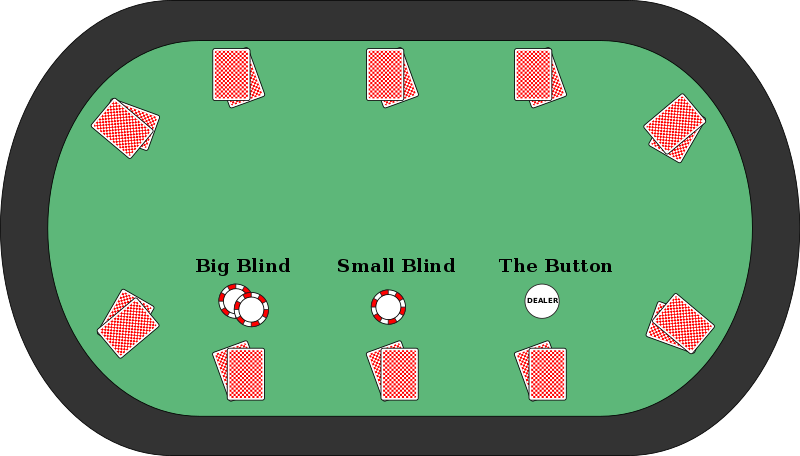
\includegraphics[width=0.90\textwidth]{figuras/Holdem_mesa.png}   
\caption{Diagrama de la distribución de las ciegas en cada partida.\cite{holdem_mesa}}
\label{fig:mesa_bids}
\end{figure}

Cuando una partida de Texas Hold'em avanza hasta el punto de que sólo queden dos jugadores en la partida, o en el caso de que se esté jugando en la modalidad \textit{heads-up} (partidas de dos jugadores), el jugador que sea el \textit{Dealer} tiene que realizar la ciega grande y el otro jugador (el jugador inicial) tiene que hacer la ciega pequeña.

Además de las apuestas ciegas, se pueden añadir apuestas obligatorias a todos los jugadores conocidos como \textit{Ante}, que es una apuesta obligatoria a todos los jugadores adicional a las apuestas ciegas para forzar a todos los jugadores a tener que arriesgar algo de dinero en cada ronda. En los torneos competitivos, tanto las apuestas ciegas como los \textit{Antes} van incrementándose a medida que el torneo avanza.\footnote{Al igual que pasa con el Rastrillo, los \textit{Antes} no se van a modelar, pues son un elemento añadido por los casinos y torneos.}

Una vez que el \textit{Dealer} ha sido designado y se han realizado las apuestas ciegas, cada jugador en la mesa recibe dos cartas boca abajo, llamadas \textit{Hole Cards} o \textit{Pocket Cards}, que serán las únicas cartas que recibirá cada jugador individualmente. 

Tras repartir las dos cartas a cada jugador, comienza la primera ronda de apuestas, conocida como \textbf{Preflop}. El primer jugador en apostar durante el \textbf{Preflop} es el jugador a la izquierda de la ciega grande. Tras acabar el \textbf{Preflop} y, si quedan al menos dos jugadores, se pasa a la siguiente fase. 

La siguiente ronda se llama \textbf{Flop}, en la que se quema una carta y se ponen tres cartas boca arriba en el centro de la mesa. Tras realizar el \textbf{Flop} se realiza una nueva ronda de apuestas, empezando por el jugador a la izquierda del \textit{Dealer}.


Una vez finalizada la ronda de apuestas del \textbf{Flop}, comienza la siguiente fase de la ronda, conocida como \textbf{Turn}.


Durante el \textbf{Turn} se quema la primera carta del mazo y después se revela una carta, que se coloca a la derecha de las tres cartas reveladas durante el \textbf{Flop}, siendo la cuarta carta revelada. Después de revelar la carta, comienza una nueva ronda de apuestas, empezando por el jugador a la izquierda del \textit{Dealer}.


Al acabar la ronda de apuestas del \textbf{Turn}, comienza la fase conocida como \textbf{River}, que tiene un funcionamiento similar a \textbf{Turn}: se quema la primera carta del mazo y se revela la siguiente carta del mazo, habiéndose revelado la quinta y última carta común a todos los jugadores. Tras revelar la carta, comienza la última ronda de apuestas, empezando por el jugador a la izquierda del \textit{Dealer}.


Al finalizar esta última ronda de apuestas, comienza la fase final de la ronda, conocida como \textbf{Showdown}. Durante el  \textbf{Showdown} cada jugador que siga en la ronda revela su mano y el jugador que tenga la mejor jugada gana, llevándose el total del dinero apostado (conocido también como \textit{pot}). Los tipos de jugadas y el orden deestas se explica en el apartado \ref{sec:class}.

Cabe destacar que el \textbf{Showdown} no siempre llega a suceder, ya que tiene que ocurrir que, al menos, dos jugadores terminen las  4 rondas de apuestas. Cuando no se llega al \textbf{Showdown}, el ganador es el único jugador que no haya pasado, independientemente de la mano que tenga.

\begin{figure}[h]
\centering
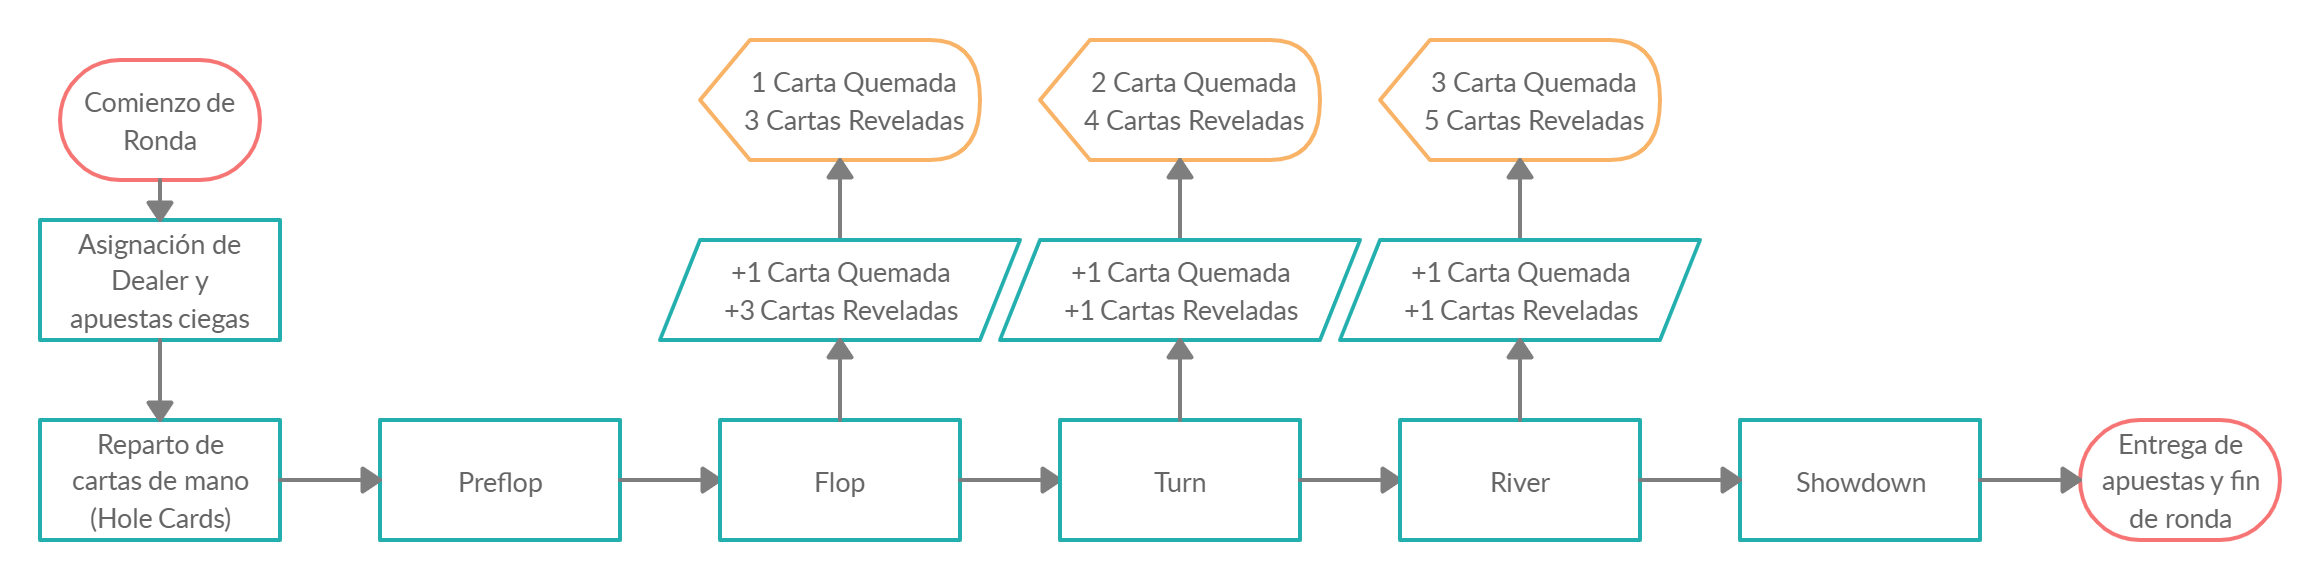
\includegraphics[width=0.9\textwidth]{figuras/Grafo3.png}   
\caption{Diagrama de la secuencia de una ronda de juego \cite{propiaCreately}}
\label{fig:bids}
\end{figure}

En resumen, el desarrollo de cada ronda de juego completa (suponiendo que, al menos, 2 jugadores apuestan en todas las rondas de apuestas) es el siguiente:
\begin{enumerate}
\item Entrega del \textit{Button}, apuestas ciegas y \textit{Antes} (en caso de que los haya)
\item Reparto de cartas iniciales (\textit{Hole Cards} o \textit{Pocket Cards})
\item Ronda de apuestas de \textbf{Preflop}
\item \textbf{Flop}: 1 carta quemada y 3 cartas reveladas.
\item Ronda de apuestas de \textbf{Flop}.
\item \textbf{Turn}: 1 carta quemada y 1 carta revelada.
\item Ronda de apuestas de \textbf{Turn}.
\item \textbf{River}: 1 carta quemada y 1 carta revelada.
\item Ronda de apuestas de \textbf{River}.
\item \textbf{Showdown}.
\end{enumerate}
 

\subsection{Clasificación de jugadas}
\label{sec:class}

Se conoce como jugada a la combinación de 5 cartas a partir de las cartas disponibles en una partida de Texas Hold'em tras el \textbf{Flop}. Los jugadores, durante la ronda de juego, formarán la mejor jugada con las 7 cartas que están a su disposición al final de la ronda, y compararán su jugada con la del resto de jugadores durante el \textbf{Showdown} . Para determinar la jugada, se han establecido las posibles jugadas, así como el orden de estas.  \cite{bridge}

Considerando que el número total de combinaciones es $\binom{52}{5}=$ 2.598.960, por lo que hay que tener en cuenta el número de posibles jugadas dentro del mísmo tipo. Estos datos se utilizarán en el apartado \ref{sec:prob_jug}, apartado en el que se calculará la probabilidad de cada una de las jugadas.

La siguiente tabla recoge las jugadas en orden descendente de valor, es decir, de la jugada más importante a la menos importante. 

\begin{longtable}[c]{|c|m{4em}|m{8em}|c|c|c|}
\hline
\rowcolor{lightgray} Orden & Nombre & Descripción & Ejemplo &  Freq.Absoluta & Frec.\\ \hline
1 & Escalera Real \textit{Royal Flush}&Cinco cartas del mismo palo del As al 10  &\textcolor{red}{A$\varheartsuit$K$\varheartsuit$Q$\varheartsuit$J$\varheartsuit$10$\varheartsuit$}& $\binom{4}{1}$ & 4 \\
\hline
2 & Escalera de Color \textit{Straight flush}&Cinco cartas consecutivas del mismo palo. En caso de empate, la carta más alta gana\footnotemark.  &9$\clubsuit$8$\clubsuit$7$\clubsuit$6$\clubsuit$5$\clubsuit$& $\binom{10}{1}\binom{4}{1}-\binom{4}{1}$ & 36 \\
\hline
3 & Póker \textit{ Four of a kind}&Cuatro cartas del mismo valor. En caso de que varios jugadores tengan póker, gana el póker de cartas más altas.  & \textcolor{red}{7$\varheartsuit$7$\vardiamondsuit$}7$\clubsuit$7$\spadesuit$2$\clubsuit$ & $\binom{13}{1}\binom{12}{1}\binom{4}{1}$ & 624 \\
\hline
4 & Full \textit{Full House}&Una combinación de un trío y una pareja. En caso de que varios jugadores tengan Full, gana el que tenga el trío más alto, y, en caso de que tengan el mismo trío, el que tenga la pareja más alta. &6$\clubsuit$6$\spadesuit$\textcolor{red}{6$\vardiamondsuit$10$\varheartsuit$}10$\clubsuit$ & $\binom{13}{1}\binom{4}{3}\binom{12}{1}\binom{4}{2}$ & 3.744 \\
\hline
5 & Color \textit{Flush}&Cinco cartas del mismo palo. En el caso de que varios jugadores tengan Color, gana el jugador con la carta más alta de ese palo.  & \textcolor{red}{K$\vardiamondsuit$8$\vardiamondsuit$7$\vardiamondsuit$6$\vardiamondsuit$4$\vardiamondsuit$}& $\binom{13}{5}\binom{4}{1} - \binom{10}{1}\binom{4}{1}$ & 5.108 \\
\hline
6 & Escalera \textit{Straight}&Cinco cartas consecutivas de palos diferentes. En caso de que varios jugadores tengan Escalera, gana el jugador con la carta más alta de la escalera.\footnotemark[\value{footnote}]& \textcolor{red}{Q$\vardiamondsuit$J$\varheartsuit$}10$\clubsuit$9$\spadesuit$8$\clubsuit$ & $\binom{10}{1}\binom{4}{1}^5- \binom{10}{1}\binom{4}{1}$ & 10.200 \\
\hline
7 & Trío \textit{Three of a kind}&Tres cartas del mismo valor. En caso de que varios jugadores tengan Trio, gana el Trio de mayor valor & \textcolor{red}{7$\varheartsuit$7$\vardiamondsuit$}7$\clubsuit$K$\spadesuit$2$\clubsuit$ & $\binom{13}{1}\binom{4}{3}\binom{12}{2}\binom{4}{1}^2$ & 54.912 \\
\hline
8 & Doble Pareja \textit{Two Pair}&Dos parejas de cartas. En caso de que varios jugadores tengan Dobles Parejas, gana el jugador con la pareja más alta, en caso de que tengan la misma pareja alta, gana el jugador con la segunda pareja más alta. & 8$\spadesuit$8$\clubsuit$6$\spadesuit$\textcolor{red}{6$\varheartsuit$2$\vardiamondsuit$} & $\binom{13}{2}\binom{4}{2}^2\binom{11}{1}\binom{4}{1}$ & 123.552 \\
\hline
9 & Pareja \textit{Pair}&Dos cartas del mismo valor. En caso de que varios jugadores tengan Pareja, gana el jugador con la pareja más alta.  & 7$\spadesuit$7$\clubsuit$K$\spadesuit$\textcolor{red}{4$\varheartsuit$}2$\spadesuit$  & $\binom{13}{1}\binom{4}{2}\binom{12}{3}\binom{4}{1}^3$ & 1.098.240 \\
\hline
10 & Carta Alta\textit{High Card}&La carta de mayor valor &\textcolor{red}{A$\varheartsuit$}10$\spadesuit$8$\clubsuit$7$\spadesuit$2$\clubsuit$ & $[\binom{13}{5}-10][\binom{4}{1}^5-4]$ & 1.302.540 \\
\hline
\caption{Clasificación de Jugadas en Texas Hold'em}
\label{tab:jugadas}
\end{longtable}

\footnotetext{Cabe destacar que, en las escaleras, el As puede tener un doble valor (As o 1), por lo que puede formarse tanto escalera de AKQJ10 como de 5432A. En este último caso, la carta más alta sería el 5. Únicamente ocurre esto con el As, haciendo que 5432A sea la única escalera posible que incluya cartas altas y bajas (Por ejemplo, 32AKQ no sería una escalera).}

En caso de que dos jugadores tengan exactamente la misma jugada, se aplica el valor de desempate, o \textit{kicker}, que es la carta de más valor fuera de la jugada sin importar su palo. Es decir, que si tu jugada es Q-Q-A-10-3, el \textit{kicker} sería A-10-3. En caso de tener la misma jugada, se empieza a comparar las cartas del \textit{kicker} y el que tenga la primera carta más alta que el \textit{kicker} del oponente, es el ganador.  En caso de que el \textit{kicker} sea idéntico, se produce un empate y se reparte el dinero acumulado de la apuesta entre los jugadores empatados.
Es importante tener en cuenta que hay jugadas en las que el \textit{kicker} no existe, ya que la jugada implica cinco cartas: Escalera Real, Escalera de Color, Full, Color y Escalera. 
También hay una posibilidad en la que el kicker no dependa de la mano del jugador, y es que las cartas más altas fuera de la jugada se encuentren en la mesa. Se expone un ejemplo de esto:
Quedan dos jugadores en la ronda durante el Showdown:
Jugador A: A$\spadesuit$\textcolor{red}{5$\vardiamondsuit$}
Jugador B: A$\clubsuit$10$\clubsuit$
Mesa: 2$\spadesuit$ \textcolor{red}{A$\varheartsuit$} K$\spadesuit$ \textcolor{red}{Q$\varheartsuit$ A$\vardiamondsuit$}
En este caso, la mejor jugada del jugador A es A$\spadesuit$ \textcolor{red}{A$\varheartsuit$A$\vardiamondsuit$}K$\spadesuit$ \textcolor{red}{Q$\varheartsuit$} mientras que la mejor jugada del jugador B es A$\clubsuit$ \textcolor{red}{A$\varheartsuit$A$\vardiamondsuit$} K$\spadesuit$ \textcolor{red}{Q$\varheartsuit$}. Es decir, que ambos jugadores tienen el mismo kicker a pesar de tener cartas de distinto valor en su mano, por tanto, se produciría un empate entre ambos jugadores.

\subsection{Faroles}
\label{sec:bluff}

Antes de tratar de los faroles, es necesario introducir los conceptos de \textit{draw} y \textit{Made Hand}. Un \textit{draw} es una mano de cuyo valor en caso de que la ronda terminara inmediatamente no sería la mejor de todas las posibles combinaciones entre las manos restantes, pero si salen determinadas cartas (llamadas \textit{outs}), mejora hasta ser la mejor. Es decir, es una mano que no vale nada a menos que salga una de sus outs, cartas que necesita para ganar. Mientras que \textit{Made Hand} es una jugada completa (Pareja, dobles parejas, Escalera…). Frente a un \textit{draw},\textit{Made Hand} suele apostar y subir. \cite{chen}

La causa de esta variación de valor de un \textit{draw} es el hecho de que el Texas Hold'em no es un juego estático, pues información se revela y eso provoca estos cambios de valores. 

Cuando la información es asimétrica, el jugador con\textit{Made Hand} está en desventaja ya que tiene que correr riesgos en algunas de las ocasiones en las que el \textit{draw} evidente aparece. En el caso de no correr esos riesgos, los demas jugadores pueden aprovecharse del \textit{draw} usando faroles de manera agresiva.\cite{chen}

Un farol, o \textit{bluff}, es una apuesta cuando la jugada que se tiene no vale nada. En otras palabras, un farol consiste en intentar intimidar a los demas mostrando una seguridad sin una jugada que la respalde.

Los faroles son una parte intrínseca de la psicología del póker, dado que un farol puede resultar en una gran pérdida de dinero cuando se resuelve. En torno a los faroles se pueden distinguir:\cite{chen}
\begin{itemize}
\item \textbf{Farol Puro:} es una apuesta con una mano que no tiene posibilidad alguna de ganar el bote mediante una estrategia óptima del oponente. Por lo general esto ocurre en las últimas fases de la ronda, donde la mano no puede mejorar.
\item \textbf{Semifarol:} es una apuesta con una mano que pueda o no ser mejor en el momento, pero puede mejorar tremendamente en las fases posteriores.
\item \textbf{Snowing:} Es un farol puro que se hace cuando no se tiene esperanza de ganar el bote en las primeras rondas de la partida.
\item \textbf{Apuestas de valor / Value bets:} Son apuestas que se espera que tengan una expectación positiva, incluso cuando son vistas. En casos extremos, incluso cuando un jugador tiene la mejor jugada posible en las primeras rondas, puede hacer una apuesta de valor pura en esas primeras fases, pero al igual que los faroles, es frecuente el caso de que, teniendo cartas pendientes de salir, la apuesta de valor pueda ser un semifarol (dependiendo de cómo de fuerte sea la mano del oponente). \cite{chen}
\end{itemize}

\chapter{La matemática detrás del Póker: Combinatoria y Probabilidad}

\section{Probabilidad de las jugadas}
\label{sec:prob_jug}

Durante las partidas de Texas Hold’em, los jugadores tratan de obtener una jugada que resulta de combinar de cinco cartas de entre toda la baraja, resultando en un caso de combinatoria. Esto se traduce en 52 posibles cartas escogidas 5 cartas sin importar el orden y sin repetición, por lo cual se obtiene un total de $\binom{52}{2}$ = 2.598.960 posibles combinaciones. 

Partiendo de la tabla \ref{tab:jugadas}, es posible calcular las probabilidades de obtener cada tipo de jugada dividiendo el número de posibilidades entre el número de casos completos.Hay que tener en cuenta varias cosas en lo que se refiere a la baraja:
\begin{itemize}
\item El Texas Hold'em utiliza una baraja francesa estándar, por lo que la baraja contiene 52 cartas
\item Cada carta tiene la misma posibilidad de aparecer que el resto de cartas restantes del mazo.
\end{itemize}

Con esto, se puede obtener también la cuota de esa mano también conocida como \textit{odds}, que es el inverso de la probabilidad. La cuota define el el ratio de la cantidad de manos que no son la buscada.
Por ejemplo, el número de Escaleras de color posibles son 36, por lo que se puede calcular el número de casos que no son una Escalera de color (2.598.960-36=2.598.924), por lo que la cuota sería 2.598.924:36, que simplificando es 72.192,3:1.

Las cuotas se tratarán en profundidad en el apartado \ref{sec:odd}.

Ahora se procede a calcular la tabla con la probabilidad de cada una de las manos.

\begin{longtable}[c]{|c|m{4em}|m{8em}|c|c|c|}
\hline
\rowcolor{lightgray} Orden & Nombre & Ejemplo &  N & Prob(\%) & Cuota\\ \hline
1 & Escalera Real \textit{Royal Flush}&\textcolor{red}{A$\varheartsuit$K$\varheartsuit$Q$\varheartsuit$J$\varheartsuit$10$\varheartsuit$}& 4 &$1.539*10^{-4}$&649.739:1\\
\hline
2 & Escalera de Color \textit{Straight flush}&$\clubsuit$8$\clubsuit$7$\clubsuit$6$\clubsuit$5$\clubsuit$&36& $1,385*10^{-3}$&72.192,3:1\\
\hline
3 & Póker \textit{ Four of a kind}& \textcolor{red}{7$\varheartsuit$7$\vardiamondsuit$}7$\clubsuit$7$\spadesuit$2$\clubsuit$ & 624 & $2.4001*10^{-2}$&4.164:1 \\
\hline
4 & Full \textit{Full House}&6$\clubsuit$6$\spadesuit$\textcolor{red}{6$\vardiamondsuit$10$\varheartsuit$}10$\clubsuit$ &3.744&$0,1441$&693,2:1 \\
\hline
5 & Color \textit{Flush} & \textcolor{red}{K$\vardiamondsuit$8$\vardiamondsuit$7$\vardiamondsuit$6$\vardiamondsuit$4$\vardiamondsuit$} & 5.108 &$0,1965$& 507,8:1\\
\hline
6 & Escalera \textit{Straight}&\textcolor{red}{Q$\vardiamondsuit$J$\varheartsuit$}10$\clubsuit$9$\spadesuit$8$\clubsuit$ &10.200& $0,3924$&253,8:1 \\
\hline
7 & Trío \textit{Three of a kind}&\textcolor{red}{7$\varheartsuit$7$\vardiamondsuit$}7$\clubsuit$K$\spadesuit$2$\clubsuit$& 54.912 &$2,1128$&46,3:1 \\
\hline
8 & Doble Pareja \textit{Two Pair}& 8$\spadesuit$8$\clubsuit$6$\spadesuit$\textcolor{red}{6$\varheartsuit$2$\vardiamondsuit$}& 123.552 & $4,7539$&20,03:1\\
\hline
9 & Pareja \textit{Pair}& 7$\spadesuit$7$\clubsuit$K$\spadesuit$\textcolor{red}{4$\varheartsuit$}2$\spadesuit$  & 1.098.240 & $42,257$&1,366:1 \\
\hline
10 & Carta Alta\textit{High Card}&\textcolor{red}{A$\varheartsuit$}10$\spadesuit$8$\clubsuit$7$\spadesuit$2$\clubsuit$ & 1.302.540 & $50,1177$&0,995:1 \\
\hline
\caption{Probabilidad de Jugadas en Texas Hold'em}
\label{tab:prob_jugadas}
\end{longtable}


\section {Cuotas implícitas y Cuotas de Bote}
\label{sec:odd}

A la hora de definir una estrategia, es decir, a la hora de decidir qué decisiones tomar, se tienen numerosos factores a tener en cuenta. En el Texas Hold’em, es tremendamente difícil especificar una estrategia, debido a la cantidad de posibles caminos combinatorios (1326 posibles manos iniciales, 19600 posibles combinaciones de 3 cartas en el Flop, 47 cartas en Turn y 46 para River). Incluso factorizando por palos, siguen quedando más de 5 millones de combinaciones mesa/mano para tener en consideración. 

Para poder definir una estrategia, es necesario considerar varios factores. En la sección \ref{sec:bluff}, se introdujeron los conceptos de de \textit{draw} y \textit{made hand}, que son algunos de esos factores a considerar.

En la sección \ref{sec:prob_jug} se hizo una introducción de otro de esos factores: la cuota. La cuota de una jugada es el ratio de no encontrar la mano buscada. Es decir, es la diferencia del total de combinaciones y las combinaciones del tipo que se busca. Esta cuota también se la conoce como cuota en contra. Pero no es la única cuota relacionada con el póker.

Otra de las cuotas que tienen relevancia a la hora de definir una estrategia es la cuota de bote o \textit{pot odds}. Esta cuota se define como el ratio de diferencia de tamaño entre la apuesta total de una ronda de juego con la apuesta de un jugador. Es decir, cuántas veces es más grande el bote si se compara con la apuesta. Esta cuota es el inverso del cociente de la apuesta del jugador entre la apuesta total.\cite{chen}

Poniendo un ejemplo, si el Jugador A ha apostado 20 €, el Jugador B ha apostado 60€ y el bote suma 80€, la cuota de bote del jugador A sería $(\frac{20}{80})^{-1}=\frac{80}{20}=4$ mientras que para el jugador B sería  $\frac{80}{60}=1.3333$.

Esta cuota es un valor importante para poder cálcular qué se puede esperar a la hora de apostar. Es decir, si el inverso de la probabilidad de ganar el bote es menor a su cuota de bote. Este factor puede generar mucha información, pero presenta un problema.\cite{chen}

El problema de considerar únicamente las cuotas de bote es que estas cuotas no son fieles al funcionamiento real del póker, ya que los jugadores que tengan  \textit{draw} nunca ganarían dinero una vez que reciben su mano ya que la descartarían en el momento en que vieran que tienen un \textit{draw}, pues si probabilidad de ganar con esa mano es muy baja.

Sin embargo, que un jugador tenga un \textit{draw} puede dar lugar a una estrategia que, en un juego donde hay cartas ocultas, podría llegar a resultar altamente explotable. En otras palabras, el jugador con \textit{draw} puede anticipar información extrayendo valores cuando recibe el \textit{draw}. A la combinación de cuotas inmediatas y valor esperado de fases posteriores de la ronda se le conoce como cuota implícita. \cite{chen}

Poniendo un ejemplo de esto último:  \cite{chen}

Jugador A: \textcolor{red}{A$\vardiamondsuit$K$\vardiamondsuit$}

Jugador B: 8$\clubsuit$ 7$\clubsuit$

Flop: A$\clubsuit$ K$\spadesuit$ 4$\clubsuit$

Bote preflop: 135 €

Apuesta del jugador A en Flop: 30€

Límite de apuesta: 30-60€

Se puede observar que el Jugador A tiene dobles parejas de AK mientras que el jugador B tiene un \textit{draw} de Color, a falta de una carta de $\clubsuit$. El jugador A no está seguro si el jugador B tiene \textit{draw} o no, pero se asume que el jugador A verá las apuestas del jugador B en cada una de las fases para continuar con el ejemplo.

Por tanto, se asume que B ve la apuesta de A y se continúa a la fase de River, con un total de 195€ en el bote. En este punto hay 3 casos posibles:
\vspace{5mm} %5mm vertical space

\textbf{Caso 1: La carta revelada en Turn es un trébol.}
\vspace{5mm} %5mm vertical space

 En este caso, el jugador B apostaría la apuesta alta (60€) en cada una de las dos fases posteriores (Turn y River), y el jugador A las vería ambas,tal y como se ha asumido. Esto suma al bote 120€ en cada una de las rondas, que contando los 195€ que tenía el bote tras el flop, el bote total es 435€. Para calcular el beneficio del jugador B, es necesario restarle al bote la cantidad apostada en cada una de las 3 rondas que se conocen(30+60+60 = 150 €), quedando un beneficio de 435-150=285 €. 

En este caso, la probabilidad de que ocurra esta situación es 
p(\textit{Trebol en Turn}) = 8/45 = 0,1778 =17,78\%.

\vspace{5mm} %5mm vertical space
\textbf{Caso 2: La carta revelada en Turn no es un trébol pero la carta revelada en River sí que es trebol}
\vspace{5mm} %5mm vertical space

En este caso, el jugador A apostaría la apuesta alta (60 €) en Turn, el jugador B la vería y en River es el jugador B el que apostaría la apuesta alta y el jugador A la vería. El beneficio sería el mismo que en el anterior caso (285 €).
La probabilidad de que ocurra este caso es la probabilidad conjunta de ambos eventos, es decir
 p(\textit{No trébol en Turn} $\cap$ \textit{Trebol en river}) = p(\textit{No trébol en turn})*p(\textit{Trebol en River}) = 37/45 * 8/44 = 0,1495 = 14,95 \%.


\vspace{5mm} %5mm vertical space
\textbf{Caso 3: Ninguna de las cartas reveladas es un trébol}
\vspace{5mm} %5mm vertical space

En este caso, el jugador A apostaría la apuesta alta (60 €) en Turn, el jugador B la vería, y en River el jugador no vería la apuesta y pasaría, obteniendo un beneficio de -30-60=-90€.
La probabilidad de que ocurra es el opuesto a que ocurra cualquiera de los otros dos casos, es decir\cite{chen}
p(\textit{ningún trébol}) =(37/45)*(36/44) = 1- (8/45 + 37/45*8/44) = 0.6727 = 67.27 \%.

Teniendo estos tres casos, se puede calcular el valor esperado ponderado para cada uno de estos casos, siendo el valor ponderado la multiplicación del valor por la probabilidad. Con esto, se puede elaborar la siguiente tabla:
\begin{longtable}[c]{|c|c|c|c|}
\hline
\rowcolor{lightgray}Salida & p(\textit{Salida}) & Valor (Beneficio) & Valor Esperado Ponderado\\
\hline
Trebol en Turn & 0.1778&+285 €&+ 50,673 €\\
\hline
Trebol en River&0.1495&+285 €&+ 42,6075 €\\
\hline
No trébol&0.6727&-90 €&-60,543 €\\
\hline
Total & 1 & &+ 32.7375 €\\
\hline
\caption{Ejemplo de cuota implícita}
\label{tab:implied}
\end{longtable}

Al sumar los valores esperados ponderados, se encuentra que que esta ronda tiene una expectación de ganar alrededor de 32,74€. Es importante tener en cuenta la cuota implícita cuando tienes una mano con \textit{draw}, ya que hay que tener en cuenta no solo la cantidad que se pueda ganar en caso de que salgan los \textit{outs} necesarios como la cantidad que se pueda perder en caso contrario. Tampoco se puede asumir que nuestros oponentes van a seguirnos el ritmo apostando.\cite{chen}

\section{Teorema de Bayes}
\label{sec:bayes}

El Teorema de Bayes es una herramienta que permite obtener la probabilidad de un evento condicionado en otro cuando se tiene la distribución del otro evento condicionado en ese evento y una distribución marginal de probabilidad del evento buscado. \cite{chen}

Desde el punto de vista del póker, el teorema de Bayes sirve como realimentación para la toma de decisiones y las estimaciones de probabilidad, puesto que, a medida que se vaya obteniendo nueva información, permite reajustar la estimación sobre la probabilidad y las estrategias a seguir. Esto resulta de especial utilidad, en concreto, para leer las manos y las acciones del oponente. 

La clave de la aplicación del teorema de Bayes es la existencia de una probabilidad previa y la obtención de información nueva, revisando y actualizando la probabilidad con la información obtenida. A este proceso se le conoce como inferencia Bayesiana.

De cara a este proyecto, se va a utilizar el teorema de Bayes para intentar identificar a cuál de los patrones predefinidos se enfrenta el algoritmo, y corregir las acciones del mismo según a qué patrón se enfrente.

Se procede a desarrollar la fórmula del teorema de Bayes.\cite{chen}

En el Anexo \ref{ch:AxA}, se define la fórmula genérica de la probabilidad de tener dos eventos simultáneamente:


\[p(A\cap B)=p(A)*p(B | A)\]

Se reorganiza la fórmula para intentar despejar la probabilidad de B condicionado en A:

\[p(B|A)=\frac{p(A\cap B)}{p(A)}\]

También se puede definir la probabilidad de que no ocurra el evento B. En otras palabras, la probabilidad de $\tilde{B}$:

\[p(B) + p (\tilde{B}) = 1 \rightarrow p (\tilde{B}) = 1 - p(B)\]

A partir de aquí, sabiendo que se tiene que cumplir siempre p(B) + p ($\tilde{B}$) = 1, se puede expresar p(A) como la probabilidad de A condicionado en B más la probabilidad de A condicionado en $\tilde{B}$, lo que genera la fórmula del teorema de Bayes:


\[p(B | A) = \frac{p(A|B)*p(B)}{p(A|B)*p(B) + p(A|\tilde{B})*p(\tilde{B})}\]

\section{Clasificación de manos iniciales: Criterio de Sklansky-Malmuth y Fórmula de Chen}
\label{sec:chen}

En el Texas Hold'em, se puede agrupar las decisiones, es decir, las acciones que se toman en las rondas de apuesta, en dos tipos:
\begin{itemize}
\item Decisiones con una jugada ya formada. En otras palabras, teniendo al menos 5 cartas conocidas. Esto corresponde a las rondas Flop, Turn y River.
\item Decisiones sin una jugada formada, es decir, teniendo las 2 cartas iniciales (Preflop).
\end{itemize}

Para las apuestas del primer tipo, se disponen de muchos elementos, factores y más información sobre la estrategia a seguir, el potencial de la jugada, las probabilidade sde tener mejor jugada y cuántos jugadores quedan en la partida. Pero para las apuestas del segundo tipo, la cantidad de información es mucho más limitada, por lo que es necesario aplicar otro criterio para la toma de decisiones.

Uno de los criterios más extendidos, y que se va a tomar en consideración es el criterio de David Sklansky\footnote{David Sklansky es un jugador de póker profesional americano con más de 28 años de experiencia en el circuito competitivo americano, habiendo ganado 3 brazaletes de la World Series of Póker (WSOP), considerado el mejor premio no monetario que un jugador de póker puede ganar. Además de eso, es considerado una eminencia en temas de juegos de cartas y apuestas, ya que ha escrito y colaborado en 14 libros de póker, blackjack y apuestas.} y Mason Malmuth \footnote{Manson Malmuth es un jugador de póker profesional titulado con el MS en Matemáticas en la universidad de Virginia en 1975, centrado en el estudio de las matemáticas y las apuestas. Malmuth ha escrito más de 500 artículos publicados en diversas revistas y ha sido autor y co-autor de 12 libros, incluyendo “Gambling Theory and Other Topics”, en el cual demuestra por qué tan pocas personas se les dan bien las apuestas.}. \cite{sklansky}

El criterio de Sklansky-Malmuth, también conocido como Tabla de Manos iniciales de Sklansky \& Malmuth, tiene como objetivo hacer una abstracción de información en la ronda del preflop, con el fin de intentar establecer una guía que seguir en un entorno con tan poca información como es el preflop. 

Este criterio, agrupa las manos iniciales en 8 grupos de mejor a peor, además estimando una clasificación de manos dentro de cada grupo. En la nomenclatura de los grupos, hay tres cosas a tener en cuenta en la nomenclatura: si aparece una “s” en una mano, significa que esas cartas son del mismo palo, o suited; el 10 es representado con “T”, y una “x” significa cualquier número que no haya sido mencionado previamente. El ranking es el siguiente:
\begin{itemize}
\item Grupo 1: AA, KK, QQ, JJ, AKs
\item Grupo 2: TT, AQs, AJs, KQs, AK
\item Grupo 3: 99, JTs, QJs, KJs, ATs, AQ
\item Grupo 4: T9s, KQ, 88, QTs, 98s, J9s, AJ, KTs
\item Grupo 5: 77, 87s, Q9s, T8s, KJ, QJ, JT, 76s, 97s, Axs, 65s
\item Grupo 6: 66, AT, 55, 86s, KT, QT, 54s, K9s, J8s, 75s
\item Grupo 7: 44, J9, 64s, T9, 53s, 33, 98, 43s, 22, Kxs, T7s, Q8s
\item Grupo 8: 87, A9, Q9, 76, 42s, 32s, 96s, 85s, J8, J7s, 65, 54, 74s, K9, T8
\end{itemize}

El realizar esta abstracción de información reduce el número de manos posibles al 42,23\% únicamente descartando las manos que no se incluyen en ninguno de los grupos. Además, al agruparlos en 8 grupos con una jerarquía, permite establecer una guia para desarrollar una estrategia para decidir las acciones a tomar en el preflop sin tener que considerar cada una de las manos individualmente.

El problema que presenta este criterio es la necesidad de memorizar todos los grupos, y cada uno de los miembros de cada grupo. Dicho de otra manera, no está diseñado para ser tratado como un principio, es decir, que no es resumible y aplicable en unas solas frases, ya que no hay una regla para poder facilitar el recordar este criterio.
Una regla para intentar memorizar este criterio la plantean William "Bill" Chen\footnote{William “Bill” Chen es un analista cuantitativo americano, así como un jugador profesional de póker. Bill Chen, poseedor de un Doctorado en matemáticas, ha llegado a ganar 2 brazaletes del WSOP, además de haber llegado a la final de 11 torneos de la WSOP. Además de eso, ha escrito junto a Jerrod Ankenman (otro jugador de póker profesional y analista cuantitativo) el libro “The Mathematics of Póker”, además de numerosos artículos tanto en revistas como en grupos denoticias como rec.gambling.poker.} y Lou Krieger.\cite{krieger}

Entre ambos crearon la conocida como Fórmula de Bill Chen, o simplemente Fórmula de Chen. Esta fórmula sirve para dar un valor númerico a la mano con un simple vistazo a la mano inicial, ya que se basa en puntuar la carta más alta y modificar su valor en función de la segunda carta, resultando en el valor numérico de la mano.  La fórmula de Chen consiste en los unos sencillos pasos para determinar el valor de la mano:

\begin{enumerate}
\item \textbf{Carta Alta:} Se le da una puntuación a la mano en función de la carta más alta de la mano:
\begin{itemize}
\item \textbf{As}: 10 puntos.
\item \textbf{K}: 8 puntos.
\item \textbf{Q}: 7 puntos.
\item \textbf{J}: 6 puntos.
\item \textbf{10 al 2}: La mitad del valor de la carta. (10 = 5 puntos, 7 = 3.5 puntos)
\end{itemize}
\item \textbf{Pareja:}  En caso de que sean parejas, se multiplica el valor de la carta alta por 2. También se le da valor mínimo a las parejas. El valor mínimo que se da a una pareja es  5, por lo que las parejas inferiores a 5 (22, 33 y 44) su valor también es 5.
\item \textbf{Cartas del mismo palo:} Si las dos cartas son del mismo palo, se suman 2 puntos.
\item \textbf{Saltos de cartas:} En función de cuantas cartas haya entre las dos, se restan los siguientes valores:
\begin{itemize}
\item \textbf{Si hay una carta de separación (AQ, J9…): } -1 punto
\item \textbf{Si hay dos cartas de separación (AJ, J8…): } -2 puntos.
\item \textbf{Si hay tres cartas de separación (AT, J7…): } -4 puntos
\item \textbf{Si hay más de tres cartas de separación (J6, 82…), incluyendo A2, A3 y A4:} -5 puntos
\end{itemize}
\item \textbf{Bonus de escalera:} Adicionalmente, si son cartas consecutivas, o con una carta de separación, y la carta alta es menor que Q: +1 punto. Esto se debe a que permite hacer todas las escaleras altas.
\end{enumerate}

De esta manera, se pueden establecer valores, siendo estos algunos ejemplos de su fórmula:
\begin{itemize}
\item AA = 20 puntos (10 x 2)
\item AKs = 12 puntos (10 puntos del As +2 por ser del mismo palo)
\item J9 = 6 puntos (6 puntos del J -1 por la carta de separación + 1 por el bonus de escalera)
\end{itemize}

En su post, Chen recuerda que esta fórmula solo te dice qué manos deberías jugar, en ningún momento te dice en qué momentos apostar o no. Por su experiencia, Chen jugaría determinadas manos según en qué posición tenga en esa ronda:

\begin{itemize}
\item Inmediatamente después del jugador con la Ciega Grande (posición conocida como “Under the gun”): manos de 8 o más puntos. 
\item En las posiciones medias (las tres posiciones después de “Under the gun): manos de 7 o más puntos.
\item En las posiciones finales (las dos posiciones a la derecha del Dealer): manos de 6 o más puntos
\item Siendo el Dealer: 5.5 o más puntos.
\item Siendo la Ciega Grande: 5.5 o más puntos.
\item Siendo la Ciega pequeña: 5 o más puntos si nadie ha subido la apuesta. Si ha habido subida, dependiendo de la situación
\end{itemize}


Además, también trata en qué situaciones puedes subir la apuesta inicial y en qué manos ver una resubida (es decir, que suban tu apuesta una vez se ha subido la apuesta). Para subir una apuesta o ver una subida, recomienda manos de al menos 10 puntos, mientras que para ver una resubida recomienda manos de 12 puntos.
Disponiendo de ambos criterios (Sklansky \& Malmuth y Formula de Chen), se ha realizado la tabla \ref{fig:sklansky} cruzando ambos criterios y establecer un patrón común, siendo la leyenda de colores los grupos de la tabla de Sklansky \& Malmuth la figura \ref{fig:Leyenda}.

De esta manera, se pueden agrupar los valores de ambos criterios y, con un único vistazo, poder hacer una idea intuitiva de qué manos son mejores según ambos criterios. 

El procedimiento de abstracción que genera la fórmula de Chen tiene bastante similitudes con las Reglas de Puntuación o \textit{Scoring Rules}. Las reglas de puntuación son una herramienta de la teoría de decisiones que sirve para medir la precisión de predicciones probabilísticas, especialmente a aquellas que se centren en asignar probabilidades a un conjuto de resultados excluyentes, que utiliza diversos criterios de puntuación para generar un resultado. Esta medida que se genera se puede considerada una medida de calibración le dichas predicciones probabilísticas.

\begin{figure}[h]
\centering
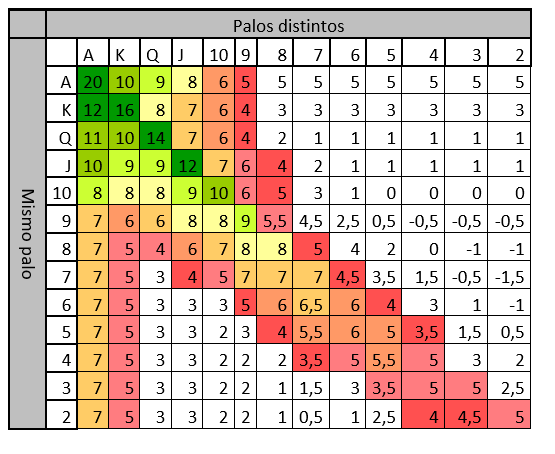
\includegraphics[width=0.8\textwidth]{figuras/chen-sklansky.png}   
\caption{Cruce de criterio de Sklansky-Malmuth con Fórmula de Chen.\cite{propiaChen}}
\label{fig:sklansky}
\end{figure}

\begin{figure}[h]
\centering
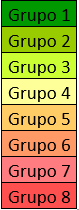
\includegraphics[width=0.1\textwidth]{figuras/grupos.png}   
\caption{Leyenda usada en la figura \ref{fig:sklansky}. \cite{propiaChen}}
\label{fig:Leyenda}
\end{figure}


\chapter{Fundamentos Matemáticos y  de programación}

\section{Aleatorización en programación: Números pseudoaleatorios y Fisher-Yates}

La utilidad de los números generados al azar es innegable, pues sirve de interés en muchos ambitos, tales como la toma de decisiones o la programación. Pero definir un número aleatorio es mucho más dificil de lo que parece,  pues un número cualquiera puede ser aleatorio o no según el contexto. En lugar de eso, es necesario referise a una secuencia de números independendientes aleatorios dentro de una distribución concreta.

Esta secuencia implica que cualquiera de los números de la secuencia puede ser obtenido únicamente por el azar, sin tener ningún tipo de inferencia por parte del resto de los números de esa secuencia y cada número tiene una probabilidad específica de caer dentro de los valores definidos, siendo una distribución uniforme si esta secuencia es finita y todos los números de esa secuencia tienen la misma probabilidad.\cite{knuth} 

Desde el punto de vista de la computación estos números aleatorios se puede agrupar en dos categorías, según su origen:

\begin{itemize}
\item \textbf{Números aleatorios ''reales''.} Este tipo de números son los que se generan a partir de  de la medida de un fenómeno físico, tal como el tiempo en que se pulsa una tecla, la temperatura exacta, radioactividad....

\item \textbf{Números pseudoaleatorios.} Estos números se generan mediante un algoritmo que parte de un valor base, llamado semilla, para generar una secuencia de números. Si bien esta secuencia parece aleatoria, no lo es pues llega un punto en el que se empiezan a repetir de nuevo (aunque este sea altísimo). Por otro lado, en el caso de tener el algoritmo y conocer la semilla utilizada, se podría recrear esa misma secuencia, cosa que un número aleatorio ''real'' es prácticamente imposible. \cite{pnrg}.
\end{itemize}

El estudio que interesa desde el punto de vista de la inteligencia artificial y de este proyecto es el de los números pseudoaleatorios, del cual se va a explicar ahora con más detalle.

Las secuencias numéricas pseudoaleatorias se pueden comparar entre ellas y determinar cuál es mejor secuencia de números pseudoaleatoria. Para esto, es necesario comparar el periodo de la secuencia, es decir, cuánto tarda la secuencia en repetirse. Cuanto mayor sea el periodo, más eficiente es dicha secuencia.

Prácticamente, todos los lenguajes de programación tienen una función para generar números pseudoaleatorios (rand(), rnd(), srand()…). Pero debido  al periodo que suelen tener este tipo de funciones, cuando se llama numerosas veces en la misma ejecución a esa función aleatoria,acaban dandose repeticiones de secuencias.\cite{rand}. 

Para poder solventar este problema, es necesario buscar un generador de números pseudoaleatorios con un periodo lo suficientemente grande para que no sea posible que se produzca la repetición.

Se denomina generador de números pseudoaleatorios (GPAN) al algoritmo encargado de generar una secuencia de números pseudoaleatorios, mientras que un Generador hardware de números aleatorios (HRNG) es el encargado de generar los números aleatorios "reales".

Para este proyecto, se ha decidido usar como GPAN el algoritmo Keep It Simple Stupid (KISS) , en concreto la versión la versión de 2009 de 64 bits. Este algoritmo fue presentado por George Marsaglia (matemático y científico computacional) y ha ido mejorando sus versiones desde su primera versión publicada en 1998. El algoritmo KISS combina 3 o 4 (dependiendo de la versión) GPAN distintos para intentar mejorar el factor de aleatoriedad.

La versión que se ha decidido utilizar combina una multiplicación con acarreo (MWC), un Generador Lineal Congruencial (CNG) y un Xorshift (XS) El algoritmo KISS sigue la siguiente formula:\cite{kiss2,kiss1}

\begin{verbatim}
Siendo xs y carry valores definidos y cng la semilla
CNG()
XS()
Definicion MWC()
KISS = MWC() + CNG+ XS.
\end{verbatim}

Con esto se obtendría el valor KISS, en función de la semilla. En el caso del proyecto, se ha implantado una función de calentamiento que ejecute n veces el algoritmo y un modificador de semilla.
Para producir un número pseudoaleatorio, se ejecutan las siguientes funciones:

\begin{verbatim}
Dado n.
inicializa_semilla_inicial()
.funcion_calentamiento(n)
s<-valor KISS n+1
inicializa_semilla(s)
k<-valor KISS (semilla s)
\end{verbatim}
\section{Aprendizaje Automático y Lenguaje R}

Uno de los objetivos iniciales es desarrollar una inteligencia artificial que sea capaz de asimilar esa información y ser capaz de procesarla, dando lugar a una decisión. Esto puede ser recogido como aprendizaje automático. El aprendizaje automático es una rama de la inteligencia artificial centrada en la búsqueda de técnicas para que el rendimiento de una máquina mejore con su funcionamiento (es decir, que “aprendan” a medida que van funcionando). El objetivo de esta rama es encontrar patrones y algoritmos que permitan replicar el comportamiento de la máquina en otro conjunto de datos.

 Este proyecto trata de emular dicho aprendizaje automático y desarrollar un algoritmo que podría ser el resultado del aprendizaje automático, así como hacer las pruebas de este. Para lograr este desarrollo, toda la programación del algoritmo se realizará en lenguaje R.
R es un lenguaje y entorno de programación para computación estadística y gráfica. Siendo un proyecto GNU, es un software libre que permite su funcionamiento en cualquier sistema operativo. 

R posee una gran capacidad de manejo y almacenamiento de datos, operadores para matrices, una gran colección de herramientas de análisis de datos, así como un lenguaje de programación efectivo que permite realizar bucles, comparaciones condicionales y funciones recursivas, así como una gran cantidad de herramientas tanto estadísticas como gráficas (tales como modelado lineal y no lineal, análisis de series temporales, análisis de grupos y clasificaciones).\cite{r-project}

\section{Optimización y Patrones de juego}
\label{sec:opti}

Las personas tienden a comportarse siguiendo uno o varios patrones de manera subconsciente, y esto también se aplica en los juegos. 
Uno de los elementos clave a la hora de optimizar el estilo de juego y, por ello, obtener mejores resultados es la predicción del comportamiento de juego. En otras palabras, ser capaz de identificar patrones de comportamiento de otros jugadores y actuar en consecuencia.
Los jugadores profesionales de póker intentan mejorar esto y hacer predicciones con la información que van obteniendo de prácticamente cualquier factor posible, tales como las acciones que toman, la rapidez en tomar decisiones, el tiempo que sopesan antes de hacer una jugada, el importe de las apuestas o incluso algún indicio de nerviosismo como tics nerviosos.
Además de esto, los jugadores profesionales tienden a cambiar constantemente de patrón a la hora de jugar rondas para intentar evitar que sus oponentes sean capaces de predecir sus acciones.
Por otro lado, hay jugadores que juegan de manera muy pobre en lo que se refiere a la obtención de información, ocultar información y descifrar esta información de los oponentes. Este tipo de jugadores son los que suelen seguir un patrón de juego y son fácilmente de identificar por jugadores profesionales, por lo que es relativamente fácil jugar en torno a ellos. 
Estos jugadores pueden diferenciarse en numerosos tipos, según sean sus patrones. Además, cada jugador profesional suele hacer sus propias clasificaciones de patrones. 

Este proyecto va a centrarme en algunos de estos patrones, que están explicados en The Mathematics of Póker\cite{chen}, en el capítulo de juego explotador. 
Estos patrones son:

\begin{itemize}
\item \textbf{Maniaco}

Este patrón se caracteriza por ser un comportamiento tremendamente agresivo, subiendo manos de manera bastante agresiva, incluso aun no teniendo una mano adecuada para ello. 

Citando la obra de Sklansky-Malmuth, “A maniac is a person who not only plays much more than his appropiate share of hands, but also constantly raises and reraises, even though the hand he holds does not warrant it. Although the maniac eventually will go broke, he does pose a set a problems for you”\cite{sklansky}, traducido como “un maniaco es una persona que no solo juega muchas más manos que las manos adecuadas, sino que también sube y resube, incluso aunque la mano que tenga no lo permitiría. A pesar de que el maniaco eventualente se quedará sin dinero, nos supone una serie de problemas”. 
En otras palabras, que va a jugar bastantes más manos de lo habitual. Y haciendo subidas de manera mucho más arriesgada. 
Este patrón consigue beneficios a raíz de forzar subidas de apuestas, y que otros jugadores no puedan seguirle el ritmo apostando y se acaben retirando. Por el contrario, si los jugadores no siguen su ritmo de apuestas, suele perder bastante fuerza. También es débil ante jugadores con buenas manos en la ronda, ya que el maniaco sube su apuesta aunque no tenga una buena jugada.

\item \textbf{Roca}

A diferencia del patrón anterior, este patrón se caracteriza por un comportamiento principalmente pasivo, siendo muy cauto a la hora de actuar. 
Este tipo de jugadores juegan únicamente en torno a su mano, únicamente jugando manos que saben que son fuertes. Este tipo de jugadores rara vez hacen faroles, así como tienden a valorar únicamente la mano actual sin analizar su potencial. Esto hace que se pierdan manos potencialmente buenas solo para mantener el estado de juego seguro.
La principal ventaja de este patrón es que el modelo es la fortaleza de sus jugadas, soliendo ganar las pocas manos que juega. Por el contrario, al no jugar muchas manos, suelen acabar perdiendo dinero con las apuestas ciegas y el ante en caso de que lo haya. También, por esa pasividad, suele pasar manos con potencial si el oponente juega agresivo y pueda parecer que tiene mejor mano.

\item \textbf{Calling Station}

Este tipo de jugadores tienen un estilo similar al del maniaco, pero menos agresiva. Se podría considerar una versión intermedia entre Roca y Maniaco. Los jugadores con un patrón calling station ven muchas apuestas, aunque la mano que tienen no deberían hacerlo. Esto hace que tenga peores resultados que Maniaco ya que, al no subir apuestas como un Maniaco, no genera tanta presión a sus adversarios.
Si bien es cierto que ver manos suele ser de utilidad para extraer información de los demás jugadores, cuando se convierte en un patrón es peligroso, ya que es muy fácil de identificar frente a los otros dos por ser repetitivo y pasivo. 
\end{itemize}

\section{REST API}

Para este proyecto se utilizará como enlace un planteamiento REST API para conectar el algoritmo con el motor de juego.  Para empezar, se procede a explicar en qué consiste una API.

Una API (del inglés “Application Protramming Interface”, que significa Interfaz de programación de aplicaciones) es una interfaz de computación  que sirve como “intermedario” para  que dos aplicaciones  se comuniquen entre ellas.   
En otras palabras, es el conjunto de funciones, métodos, subrutinas y procedimientos que permite utilizar un software desde otra aplicación como una abstracción de la implementación ,  creando así una “librería” disponible para ese software.
Esta interfaz facilita mucho el trabajo a la hora de programar, pues únicamente muestra el código estrictamente necesario, ocultando muchos comandos que se ejecutan implícitamente. \cite{api1}

Dentro de las APIs,  se encuentra un  tipo de API  que permite una manipulación más sencilla de datos que el resto. Se trata de la API REST.
REST es cualquier API entre sistemas que, mediante el uso del protocolo HTTP, permita obtener datos o generar operaciones sobre estos datos en cualquier formato posible, entre los cuales encontramos XML y JSON. 

Este tipo de API permite la separación total entre el cliente y el servidor, además, es independiente del tipo de plataformas y lenguajes, por lo cual su implementación entre dos lenguajes distintos es posible e, incluso, bastante sencilla. Como tiene esa adaptabilidad de sintaxis, ofrece bastante flexibilidad a la hora de programar un API en múltiples lenguajes. 
Las características generales de una REST API son las siguientes:\cite{api2}
\begin{itemize}
\item Protocolo cliente/servidor sin estado: Cada una de las peticiones del API tiene toda la información necesaria para ejecutarla, por lo que no necesita recordar ningún estado previo para satisfacer esta petición (ni el cliente ni el servidor). Es posible configurarlas para que tengan caché, creando lo que se conoce como protocolo cliente-caché-servidor sin estado.
\item Operaciones bien definidas: Un REST API tiene un conjunto pequeño de operaciones relacionadas con datos y especificación HTTP. Las más importantes son POST (crear), GET (leer y consultar), PUT (editar) y DELETE (eliminar).
\item Sintaxis universal: los objetos en una API REST siempre se manipulan a partir de la URI.  Esta UIR es un elemento identificador único para cada recurso en la API REST. Lo cual permite acceder siempre de manera exacta a la información. Esta sintaxis universal a su vez genera una interfaz uniforme, que implica que un sistema REST siempre aplica acciones concretas sobre los \item Uso de hipermedios: tanto para la información de la aplicación como para las transiciones de estado de la aplicación, la representación suele ser en HTML o XML, lo que permite navegar de un recurso REST a muchos otros, simplemente siguiendo los enlaces sin necesidad de una infraestructura adicional.
\end{itemize}



\chapter{Desarrollo del proyecto : Simulador de juego}

\section {Abstracciones, decisiones y simplificaciones}
\label{sec:abstracciones}

A la hora de plantearse el desarrollo del proyecto, se ha comenzado tomando una serie de decisiones a la hora de diseñar el proyecto. 

La primera decisión procede de la estructura del diseño. La primera decisión tomada con respecto a esto es que el algoritmo funcione como una caja negra para el motor de juego, es decir, que independientemente de cómo sea el funcionamiento del algoritmo no influya para nada en el código del motor de juego. 

Siguiendo este hilo de razonamiento, se ha decidido que el motor de juego y el algoritmo se programen en medios separados, conectados entre ambos y que, cuando el motor de juego lo necesite, se llame al algoritmo para la toma de decisiones mediante esa conexión.
El esquema visual de este planteamiento sería el siguiente:
 
\begin{figure}[h]
\centering
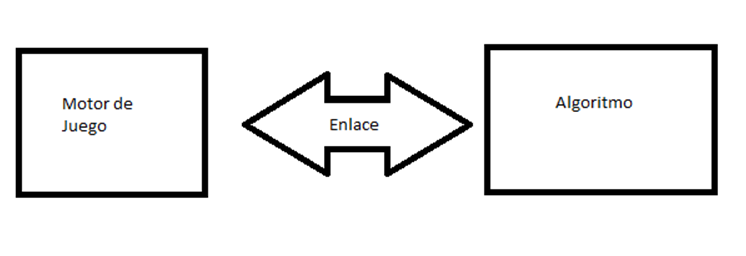
\includegraphics[width=0.45\textwidth]{figuras/esquema.png}   
\caption{Diagrama de diseño del modelo de funcionamiento \cite{propiaPaint}}
\label{fig:esquema}
\end{figure}

Con esta idea en mente, se puede proceder a las elecciones de los medios para programar. En lo que se refiere a los medios utilizados, las elecciones han sido las siguientes:
 \begin{itemize}
\item El motor de juego se ha desarrollado en C++ utilizando Visual Studio 2019. 
\item El algoritmo, las probabilidades y todas las iteraciones se han desarrollado en lenguaje R utilizando la versión R 4.0.0
\item El enlace se ha implementado usando un API REST, con parte programada en C++ y otra en R.
\end{itemize}

Se ha  decidido usar esos lenguajes de programación por comodidad, pues es con los que más tiempo se ha trabajado previamente.

Una vez establecidos los medios a utilizar, es necesario plantearse algunas abstracciones con el fin de simplificar el código a desarrollar, la matemática y, en general, todo el proyecto.

 \begin{itemize}
\item El juego se realizará en la modalidad de \textit{Heads-up}, es decir, el número de jugadores será 2: jugador0 y jugador1. Esta simplificación se hace por varios motivos:
 \begin{itemize}
\item Se limita la información a modelar, ya que las únicas variables ocultas de otros jugadores es un conjunto de 2 cartas.
\item Se limita el número de modelados, ya que solo es necesario modelar a un oponente.
\item Se eliminan factores como la posición con respecto al \textit{Dealer}, lo que facilita desarrollar una estrategia de juego.
\end{itemize}
\item Tal y como se había adelantado en el apartado \ref{sec:choices}, el juego elegido es Texas Hold'em. Como tipo de apuestas, será una apuesta sin límite. En otras palabras, las partidas serán en HUNL(Heads-Up No-Limit) Texas Hold'em.
\item El jueego tendrá dos modos de juego: 
\begin{itemize}
\item Jugador vs Máquina, en el cual un jugador controla al jugador0 para enfrentarse al algoritmo diseñado, que controlará al jugador1. Esta modalidad tiene una funcionalidad principalmente de pruebas de funcionamiento
\item Máquina vs Máquina, en el cual el motor de juego juega solo, que generará un registro con todas las acciones y el resultado de cada mano en beneficio neto. Este modo tiene dos opciones: Algoritmo vs Patrón, donde el Algoritmo se enfrentará a un patrón a la elección del jugador, y Patrón vs Patrón, donde puede hacerse que se enfrenten los Patrones predefinidos entre ellos.
\item El enlace se ha implementado usando un API REST, con parte programada en C++ y otra en R.
\end{itemize}
\item El dinero inicial, así como el valor de la Ciega Grande se podrá introducir manualmente. Para las pruebas de este algoritmo se han utilizado una cantidad constante (10000 de dinero inicial y 20 de ciega grande). Se han tomado estas cantidades a las pruebas para mantener una proporción de 500:1 entre dinero inicial y ciega grande. Cabe destacar que el valor de la ciega grande es una unidad estándar para medir los valores de ganancia en una partida.
\item Los elementos de apuestas relacionados con los casinos se suprimen. Es decir, el \textit{Ante} y el \textit{Rake}. Estos dos elementos no influyen en la probabilidad de las acciones de juego. Si bien el \textit{Ante}  pueda llegar a ser considerado un posible factor a la hora de tomar algunas estrategias, su relevancia solo aparece en situaciones límite, por lo que en la mayoría de los casos solo supone una dificultad añadida a la hora de gestionar las apuestas. Lo mismo pasa con el \textit{Rake}, salvo que este elemento no tiene importancia alguna ni en la probabilidad ni en la estrategia de juego, por lo que lo único que aporta son complicaciones a la hora de programar.
 \begin{itemize}
\item A modo adicional, la eliminación del \textit{Rake} conviere al juego en un juego Suma-Cero, es decir, que las ganancias o pérdidas de un jugador se equilibra perfectamente con las ganancias o pérdidas de los demás jugadores. Al ser un HUNL póker, esto se traduce como las pérdidas de uno de los dos jugadores son las ganancias del otro jugador.
\end{itemize}
\item Se modela el quemado de cartas. Si bien este elemento no influye en la probabilidad ni en la estrategia, es un elemento más del Hold'em y es totalmente inócuo al flujo de juego, por lo que no complica la programación, así que se modela únicamente por similitud con el juego original.
\item Se limita el número de subidas en una misma ronda de apuestas a 3. Esta decision se toma principalmente por optimización de tiempo de ejecución, y para evitar que haya bucles infinitos de cara al modo Máquina vs Máquina.
\item El número de manos máxima será definido al comienzo de las iteraciones, por lo que será un número limitado.
\item La partida acaba cuando ocurra, al menos, una de las siguientes situaciones:
\begin{itemize}
\item El dinero de uno de los dos jugadores llega a 0
\item En el modo de Jugador vs Algoritmo, cuando el jugador desee finalizar la partida.
\item En el modo de Máquina vs Máquina, cuando se alcance el número de iteraciones deseadas.
\end{itemize}
\end{itemize}

\section {Cuantificación de las jugadas}
\label{sec:valmano}

Con el fin de simplificar el cálculo de jugada obtenida, se ha decidido cuantificar las posibles jugadas, otorgándole un valor numérico (usando variables de tipo float en el motor de juego, y un valor entero en el algoritmo)\footnote{Esta diferenciación se hace porque el algoritmo necesita comparar jugadas iguales a la suya, añadiendo el \textit{kicker} haría practicamente imposible el igualar una mano, salvo en contadas ocasiones. En el motor de juego si que es necesario mantenerlo pues es necesario determinar un ganador.} durante el código. También se cuantifica el valor de desempate o \textit{kicker}. Esto permite al código comparar numéricamente  las jugadas de los dos jugadores, y permite establecer si una jugada es superior a otra con bastante facilidad.

Para cuantificar estas jugadas, se ha decidido otorgar un valor entero de 0 a 9 a las distintas jugadas (siendo el 9 la Escalera Real y el 0 Carta más alta). En el simulador se le ha sumado decimales que caracterice el valor dentro de su jugada y la diferencie de otras jugadas del mismo tipo, siempre que sea posible (por ejemplo, en una Escalera, el valor de la carta más alta) e incluya el desempate para cada jugada.  Se ha tomado la decisión de utilizar estos valores para hacer una comparación sencilla de computar (0 a 9, sin necesidad de usar una segunda cifra para las jugadas, y decimales para el desempate, permitiendo comparar de manera más sencilla dos jugadas del mismo tipo).

Se toman estos valores numéricos para poder categorizar las 10 posibles jugadas de manera numérica de una manera uniforme, aunque la frecuencia con la que aparecen dichas manos sea muy diversa, para poder hacer una comparación entre las jugadas. Estos valores podrían tomar cualquier valor, siempre que se mantenga un esquema para diferenciar estas 10 posibles jugadas y poderlas comparar.

Se desarrolla la tabla de la siguiente forma, incluyendo en cada jugada sus correspondientes valores característicos y desempates si aplican.

\begin{longtable}[c]{|c|c|m{3em}|m{8em}|m{8em}|}
\hline
\rowcolor{lightgray} Jugada & Estructura&  Valor Entero & Valor Caract. &  \textit{Kicker}\\ \hline
Escalera Real &9&9&-&-\\
\hline
Escalera de Color&8,AA&8& A = valor de carta más alta x$10^{-2}$&-\\
\hline
Póker&7,AAXX& 7 & A = valor de carta repetida x$10^{-2}$&X = valor de carta más alta fuera de póker x$10^{-4}$ \\
\hline
Full&6,AABB&6&A = valor de carta del trio x$10^{-2}$   B = valor de carta de la pareja  x$10^{-4}$&- \\
\hline
Color &5,AABBCCDDEE&5&A-E = valores del color ordenados de mayor a menor x$10^{-2*i}$&-\\
\hline
Escalera&4,AA&4&A= Valor de la carta alta de la escalerax$10^{-2}$&- \\
\hline
Trío&3,AAXXYY&3 &A = Valor de la carta del trio x$10^{-2}$&X = valor de la carta más alta que no sea del trio x$10^{-4}$ Y= Valor de la segunda carta más alta que no sea del trio x$10^{-6}$ \\
\hline
 Doble Pareja&2,AABBXX& 2 &A = Valor de la carta de la pareja de más valor x$10^{-2}$ B = Valor de la carta de la pareja de menos valor  x$10^{-4}$ &X=valor de carta más alta que no sea de las parejas x$10^{-6}$\\
\hline
 Pareja & 1,AAXXYYZZ & 1& A = Valor de la carta de la pareja x$10^{-2}$&X = valor de la carta más alta que no sea de la pareja x$10^{-4}$ Y= Valor de la segunda carta más alta que no sea de la pareja x$10^{-6}$ Z= Valor de la tercera carta más alta que no sea de la pareja x$10^{-8}$  \\
\hline
 Carta Alta&0,AAWWXXYYZZ & 0& A= valor de la carta más alta x$10^{-2}$&W = valor de la segunda carta más alta x$10^{-4}$ X= valor de la tercera carta más alta x$10^{-6}$ Y= valor de la cuarta carta más alta x$10^{-8}$ Z= valor de la quinta carta más alta x$10^{-10}$ \\
\hline
\caption{Formato del valor de las jugadas en Texas Hold'em}
\label{tab:kicker}
\end{longtable}


\section {Desarrollo del Motor de Juego}
\label{sec:motor}

Para el simulador de juego, en lenguaje C++, se han creado varias clases para estructurar el código, clases en las que se profundizará en su respectivo apartado. Las clases son las siguientes:

 \begin{itemize}
\item Carta: clase base que clasifica palo, número y tiene una función para imprimir la carta por pantalla. 
\item Jugador: tiene un array de Carta (para representar las manos), funciones para gestionar su dinero y sus apuestas, así como funciones para calcular el valor de su jugada.
\item Mesa: tiene dos arrays de Carta (para representar el tablero y las cartas quemadas) y tiene tanto las funciones de gestionar los índices de la partida como de imprimir el tablero en cada ronda.
\item Mazo: tiene un array de Carta y un índice para representar la posición de las cartas. También tiene las funciones para barajar el mazo (aleatorizando la posición de las cartas) y repartir las cartas tanto a jugadores como a la mesa.
\item Algoritmo: que contiene las distintas funciones para comunicarse con el algoritmo, así como los elementos para gestionar los distintos patrones.
\item Random: Que incluye toda la programación del generador de números pseudoaleatorios Keep It Simple Stupid (KISS), así como las funciones para generar números aleatorios (tanto valores porcentuales como en enteros).
\end{itemize}

Además de eso, está el archivo principal (Póker\_Simu.cpp) que inicializa los elementos de las clases y contiene un array de objetos Jugador, englobando los dos jugadores, un elemento de tipo Mesa que representa la mesa de juego. Además, Poker\_Simu.cpp tiene todas las funciones del que participan en el flujo de la ronda de juego,las funciones de las rondas de apuestas de cada uno de los modos y las funciones para determinar ganadores

\subsection{Clase Carta}
\subsubsection{Atributos}

Cada elemento de la clase carta tiene los siguientes atributos de tipo protected:
 \begin{itemize}
\item \textit{Palo (int)}: un valor de tipo int que representa el palo de la carta. Puede adquirir los valores de 1 (Tréboles), 2 (Picas), 3 (Diamantes) y 4 (Corazones).
\item \textit{Numero (int)}: un valor de tipo int que representa el valor de la carta. Puede adquirir los valores de 1 a 13, aunque algunas funciones pueden sustituir el valor de 1 por 14 para el tema de cálculos, siendo 1 (o 14) el valor para As, 11 para J, 12 para Q y 13 para K.
\end{itemize}

Con estos dos atributos, se pueden caracterizar cualquiera de las 52 cartas de la baraja francesa, como, por ejemplo:

\begin{longtable}[c]{|c|c|c|}
\hline
\rowcolor{lightgray}Carta de la baraja &Numero&Palo\\
 \hline
9$\spadesuit$&9&2\\
\hline
\textcolor{red}{3$\varheartsuit$}&3&4\\
\hline
J$\clubsuit$&11&1\\
\hline
\textcolor{red}{9$\vardiamondsuit$}&1 ó 14 (según la función)&3\\
\hline
\caption{Ejemplos de Atributos Carta}
\label{tab:carta}
\end{longtable}

\subsubsection{Funciones}
En esta clase se recogen las siguientes funciones:
\begin{itemize}
\item \textit{Int GetPalo() / int GetNumero()}: Dado que los atributos son de tipo protected, se leen utilizando una función que tenga como salida dichos atributos.
\item\textit{ Void SetPalo(int p) / void SetNumero(int n)}: Al igual que pasa a la hora de leer los atributos, para poder modificarlos es necesario una función para poder modificarlos, dejando como valor nuevo el valor int de entrada.
\item \textit{Void imprimirCarta()}: Esta función lee los valores numéricos de los atributos de Carta e imprime una frase en función del número y el palo de cada carta.
 \end{itemize}

\subsection{Clase Jugador}
\subsubsection{Atributos}

En esta clase se incluyen los siguientes atributos:
\begin{itemize}
\item \textit{mano}: un Array de dos elementos de tipo Carta, que representan las dos cartas iniciales que tiene el jugador.
\item \textit{apuesta} y \textit{apuestaInicial}: atributos de tipo float que representan las dos apuestas del jugador, siendo apuestaInicial el valor de la Ciega que le toque apostar, y apuesta el valor de la apuesta de esa ronda.
\item \textit{Dinero}: atributo de tipo float que indica el dinero restante del jugador.
\item Conjunto de \textit{Valores\_Mano}: son 4 atributos de tipo float que representan el valor numérico de la jugada  que se tiene durante la ronda correspondiente (valor\_mano-$>$Preflop, valor\_mano\_r1-$>$Flop, valor\_mano\_r2-$>$Turn y valor\_mano\_r3-$>$River), siguiendo el esquema del apartado 3.2.
\item Conjunto de \textit{jugada\_obtenida}: son 9 atributos de tipo bool que representan qué jugada se ha obtenido, de modo de ayuda para el posterior cálculo del valor numérico.
\item\textit{ Valor\_num\_mano}: un atributo de tipo float que representa el valor numérico de la mano, para cálculos de desempate.
\end{itemize}

\subsubsection{Funciones}
Por una parte, en esta clase se tienen los siguientes pares de funciones Set() y Get(), para modificar y obtener, respectivamente el valor de dicho atributo:
\begin{itemize}
\item \textit{Carta* getMano()/setMano(Carta* c)}
\item \textit{Float getDinero()/setDinero(float f)}
\item\textit{ Float getApuestaInicial() / setApuestaInicial(float f)}
\item \textit{Float getValor()}
\item \textit{Float getApuesta () / setApuesta (float f)}: aquí cabe destacar que setApuesta obtiene la diferencia entre la apuesta actual y f, asigna el valor de f a apuesta y después hace un \textit{setDinero(dinero\_actual – diferencia).}
 \end{itemize}
Por otro lado, se tienen un conjunto de funciones Reset, cuya función sirve para devolver al estado original algunos de los atributos de la clase:
\begin{itemize}
\item \textit{resetObtenidas()}: para poner cada una de las variables del conjunto de jugada\_obtenida con el valor inicial de false.
\item \textit{ resetApuesta()}: para convertir el valor de apuesta en 0.
\item \textit{resetBool()}: para poner cada una de las variables del conjunto de jugada\_obtenida con el valor inicial de true.
 \end{itemize}
Además, se tienen las funciones del cálculo del valor de la mano:
\begin{itemize}
\item \textit{valorManoInicial()}: Utilizando la fórmula de Chen, obtiene una valoración numérica de la mano inicial durante  el Preflop.
\item \textit{valorManoR1(mesa T)/ valorManoR2(mesa T)/ valorManoR3(mesa T)}: que calcula para cada ronda el array de cartas correspondiente para dicha fase (unión de Mano y las cartas del tablero disponibles esa ronda), ordena las cartas de mayor a menor y ejecuta calculoValorJugada introduciendo como entrada ese array y un valor numérico (5, 6 o 7), en función de la ronda..
\item \textit{calculoValorJugada(carta* c, int i)}: recibiendo el array de cartas ordenadas c y un índice numérico para identificar qué ronda de juego es, hace el cálculo del valor numérico. Para ello primero contabiliza los siguientes datos:
\begin{itemize}
\item Nº de cartas repetidas: identifica si hay cartas repetidas, cuantas veces se repite una carta, el número de dicha carta y el número de cartas distintas repetidas, si los hubiera.
\item Nº de palos repetidos: identifica cuántas cartas pertenencen a cada palo. 
\item Nº de cartas consecutivas: identifica cuántas cartas consecutivas hay en el array.
 \end{itemize}
 \end{itemize}
Ahora se procede a analizar los tipos de jugada posibles y como estos tres datos son necesarios para cada una, creando esta tabla:

\begin{longtable}[c]{|c|m{8em}|m{8em}|m{5em}|}
\hline
\rowcolor{lightgray}Jugada\textbackslash Dato&Cartas Repetidas& 5 Cartas consecutivas & 5 Cartas del mismo palo\\
\hline
Escalera Real&No&Si (10-A)& Si\\
\hline
Escalera de Color&No&Si (distinto de 10-A)& Si\\
\hline
Poker&Si (4 Cartas iguales)& No & No\\
\hline
Full&Si (3 Cartas repetidas y otras dos repetidas distintas)& No & No\\
\hline
Color&No& No & Si\\
\hline
Escalera&No& Si & No\\
\hline
Trio&Si (Tres cartas repetidas)& No & No\\
\hline
Doble Pareja&Si (4 cartas repetidas dos a dos)& No & No\\
\hline
Pareja&Si (2 cartas repetidas)& No & No\\
\hline
Carta Alta&No& No & No\\
\hline
\caption{Datos necesarios para cada jugada}
\label{tab:tabla}
\end{longtable}

A partir de los datos necesarios de esta tabla y, en función de los datos obtenidos, comienza el cálculo de la mejor jugada. Primero analiza qué jugadas se han obtenido, asignando el valor true a la variable correspondiente. 
\begin{itemize}
\item En caso de que haya cartas repetidas, se almacena cuantas cartas hay repetidas y qué número de carta es el repetido. Teniendo en cuenta que son 7 cartas máximo de donde se tienen que obtener la mejor jugada (En River están las cinco cartas de la mesa más las dos que tiene el jugador), el máximo de repeticiones distintas son 3 repeticiones distintas. En función de cuantas cartas obtenidas, se dará valor true a las variables póker\_obtenida, full\_obtenida, trio\_obtenida, doble\_pareja\_obtenida y/o pareja\_obtenida.
\item Si uno de los palos repetidos tiene 5 o más cartas de ese palo, el jugador ha obtenido Color. En ese caso, almacena las cartas del palo en un array auxiliar para el color y se da el valor color\_obtenida=true.
\item Si hay, al menos, cinco cartas consecutivas, se ha obtenido Escalera. También considera el caso concreto de tener 5, 4, 3, 2 y A, que también es considerado escalera debido al valor doble del As. En caso afirmativo, almacena las cartas consecutivas en un array auxiliar para la escalera y se da el valor escalera\_obtenida=true
\item Si se da la situación en la que haya tanto 5 cartas consecutivas como 5 cartas del mismo palo, es decir ocurra  escalera\_obtenida == true y color\_obtenida == true, se comparan los arrays auxiliares y, si coinciden al menos 5 cartas, se ha obtenido una Escalera de color, dando el valor escalera\_color\_obtenida=true.
\item Si se da escalera\_color\_obtenida=true, se compara la escalera con los valores establecidos de la Escalera Real (A, K, Q, J, 10). Si coinciden esas 5 cartas con las de la escalera de color, se habrá obtenido la Escalera Real dando el valor de escalera\_real\_obtenida = true
 \end{itemize}

De esta manera, se habrá contemplado la posibilidad de cualquiera de las 9 jugadas que requieren alguna combinación de cartas (es decir, cualquier jugada que no sea “Carta alta”).
\begin{figure}[h]
\centering
\includegraphics[width=0.75\textwidth]{figuras/grafo1.png}   
\caption{Asignación de jugada\_obtenida en función de los datos obtenidos en de la jugada.\cite{propiaCreately}}
\label{fig:jugada_ob}
\end{figure}

Una vez determinados los atributos del conjunto jugadas\_obtenidas que tienen valor true, se determina mediante condiciones if la mejor jugada, y se calcula el valor de desempate, siguiendo las guias que aparecen en la tabla \ref{tab:kicker}
Se han creado los diagramas \ref{fig:jugada_ob} y \ref{fig:valor} para que sea más visual esta explicación de funcionamiento.


\begin{figure}[h]
\centering
\includegraphics[width=0.75\textwidth]{figuras/grafo2.png}   
\caption{Asignación del valor jugada correspondiente en función de jugada\_obtenida. \cite{propiaCreately}}
\label{fig:valor}
\end{figure}

Por último, se tiene la función de \textit{imprimirMano()}, para ejecutar la función \textit{imprimirCarta()} de cada una de las cartas de la mano del oponente.


\subsection{Clase Mesa}
\subsubsection{Atributos}

La clase mesa se compone de los siguientes atribuitos:
\begin{itemize}
\item Índices: son 4 atributos de tipo int, que representan índices para el flujo del juego:
\begin{itemize}
\item  \textit{indiceRonda} se utiliza para llevar el conteo de la fase de la ronda (0 para preflop, 1 para flop, 2 para turn, 3 para river y 4 para showdown).
\item  \textit{indiceTablero} indica la siguiente posición del array Tablero.
\item  \textit{indicieQuemada} indica la siguiente posición del array Quemada.
 \end{itemize}
\item Arrays de carta: son dos array de atributo Carta:
\begin{itemize}
\item  \textit{Tablero:} array de 5 elementos, que sirve para almacenar las cartas que son visibles para ambos jugadores
\item  \textit{Quemada:} array de 3 Cartas, que sirve para almacenar las cartas que se “queman”
 \end{itemize}
\item  \textit{Apuesta:} float que representa la suma total de las apuestas de los jugadores.
\item  \textit{Tablero\_juego\[11\]\[26\]:} matriz de elementos Char para la representación gráfica de la mesa de juego en el modo de jugador vs algoritmo.
\item  \textit{bool modoJ:} booleano auxiliar que adquiere el valor de TRUE si se está ejecutando el modo jugador vs Máquina.
 \end{itemize}

\subsubsection{Funciones}
Los procesos de la clase Mesa son los siguientes:
\begin{itemize}
\item Funciones de índices: un conjunto de 3 funciones para cada uno de los índices, una función reset para dejar el valor a 0, una función up que aumenta el valor en uno y una función get, para obtener el valor de ese índice:
\begin{itemize}
\item \textit{void resetIndiceTablero(),	void upIndiceTablero() y int getIndiceTablero()}: para el indiceTablero.
\item \textit{void resetIndiceQuemada(),	void upIndiceQuemada() y int getIndiceQuemada()}: para el indiceQuemada.
\item \textit{void resetIndiceRonda(),	void upIndiceRonda() y int getIndiceRonda()}: para el indiceRonda.
 \end{itemize}
\item Funciones de tablero\_juego: son las tres funciones que se encargan de gestionar todo lo relacionado con la presentación visual del juego:
\begin{itemize}
\item \textit{creaTablero():} asigna el valor ‘ ‘ a cada uno de las posiciones de la matriz.
\item\textit{ modificaTablero(jugador* J):} modifica los valores de las posiciones de la matriz para que se adapte a lo que debe mostrar en cada ronda:
\begin{itemize}
\item Preflop: Las dos cartas de la mano del Jugador
\item Flop: Las dos cartas de la mano del Jugador y las tres primeras cartas de Tablero.
\item Turn: Las dos cartas de la mano del Jugador y las cuatro primeras cartas de Tablero.
\item River: Las dos cartas de la mano del Jugador y las cinco cartas de Tablero.
\item Showdown: Las dos cartas de la mano de cada Jugador, las cinco cartas de Tablero y las tres cartas de Quemada.
 \end{itemize}
\item \textit{imprimirTablero(jugador* J) }imprime por pantalla cada uno de las posiciones de tablero\_juego, así como si un jugador ha hecho All In.
 \end{itemize}
\item Funciones de flujo de rondas: son las funciones que están relacionadas con el funcionamiento de las rondas en lo que se refiere a las variables de Mesa
\begin{itemize}
\item \textit{entregarApuesta(jugador J):} se entrega el valor de la apuesta total al jugador J, así como reinicia el valor de apuesta.
\item \textit{actualizarApuesta(jugador* J):} actualiza el valor de apuesta en función de la apuesta de cada uno de los jugadores incluidos en J.
\item \textit{finRonda(Mazo m):} reinicia el valor de apuesta y ejecuta todos los resetIndice.
 \end{itemize}
\item Funciones de conversión a Char: transforma en char los valores de número y palo de la carta C para las funciones de tablero\_juego siguiendo este criterio:
\begin{itemize}
\item \textit{Char conversorNumero(Carta c) }según el valor de getNumero() de c
\item \textit{Char conversorPalo(Carta c) }según el valor de getPalo() de c
 \end{itemize}
\item \textit{Bool continuar():} una vez acaba una ronda pregunta al jugador si desea seguir jugando o terminar el juego. 
 \end{itemize}

\subsection{Clase Mazo}
\subsubsection{Atributos}
Esta clase incluye dos atributos:
\begin{itemize}
\item \textit{Deck:} Un array de elementos Carta de tamaño 52 (representando el mazo de juego)
\item\textit{ indiceMazo:} valor int que representa el índice en el que se está trabajando dentro de Deck
\end{itemize}
\subsubsection{Funciones}
El constructor de la clase,\textit{ Mazo()}, inicializa el mazo y asigna valores de palo y numero a cada uno de los elementos de deck.
Las dos funciones que interactúan con el funcionamiento de la ronda son las siguientes:
\begin{itemize}
\item \textit{Barajar():} aleatoriza el orden de los elementos de deck utilizando los valores generados por la clase Random.
\item \textit{repartirCartas(Mesa T, Jugador* J)}: asigna el valor de las cartas tanto a cada elemento de J como a los arrays Tablero y Quemada de T.
\end{itemize}

Por último, está la función  \textit{resetIndiceMazo()}, que asigna el valor 0 al indiceMazo.


\subsection{Clase Random}
\subsubsection{Definiciones de valores}

Como se comentó en la explicación del algoritmo KISS, es necesario definir los valores que va a utilizar el algoritmo, así como los valores de las semillas. Se van a utilizar las siguientes definiciones de valores para el algoritmo.   \cite{kiss2, kiss1}
\begin{verbatim}
typedef uint64_t u64;

#define QSIZE 0x200000
#define CNG (cng = 6906969069ULL * cng + 1234567)
#define XS (xs ^= (xs<<13), xs ^= (xs>>17), xs ^=(xs<<43))
#define KISS (B64MWC() + CNG + XS)

static u64 QARY[QSIZE];
static int j;
static u64 carry;
static u64 xs;
static u64 cng;
\end{verbatim}

\subsubsection{Definiciones de valores}
Habiendo definido los valores de funcionamiento del algoritmo KISS, se pueden definir las funciones de sta clase. Primero,tiene 6 funciones que sirven para generar los números pseudoaleatorios: \cite{kiss2,kiss1}
\begin{itemize}
\item \textit{int func():} genera un número entero para la función de calentamiento.
\item\textit{ rankd\_reset():} reinicia la semilla de KISS.
\item\textit{u64 B64MWC():} función que genera un número pseudoaletorio usando el método de la multiplicación con acarreo.
\item\textit{randk\_seed():} inicia el generador KISS con la semilla inicial.
\item\textit{ randk\_seed\_manual(u64 seed)} inicia el generador KISS con la semilla introducida.
\item\textit{ u64 randk()} genera un número pseudoaleatorio usando el generador KISS.
\item\textit{randk\_warmup(int rondas):} ejecuta randk() tantas veces como el número de rondas introducido, sin devolver ningún valor, lo cual hace que la secuencia avance.
 \end{itemize}
Tras eso, se tienen las 2 funciones para generar números usando ese algoritmo en el formato que resulta de utilidad para el código (ya que KISS trabaja con valores ULL).
\begin{itemize}
\item \textit{Float nrandomPorcert():} genera un número comprendido entre 0 y 1 utilizando el algoritmo.
\item\textit{ Float nrandomN(int n):} genera un número comprendido entre 0 y n.
 \end{itemize}

\subsection{Clase Algoritmo}
\label{sec:algmoto}
\subsubsection{Atributos}


Los atributos de esta clase incluye el valor \textit{int tipo}, que representa el patron o el algoritmo elegido (que se selecionará en la función Main de Póker\_simu.cpp, descrito más abajo), el valor \textit{ bool pasa}, que representa cuando el algoritmo ha decidido pasar, y el \textit{int acción}, que representa qué acción ha sido la última en tomar el algoritmo (0=pasar, 1=ver, 2=subir).
Por último, se tiene el atributo \textit{triple}, que es un array de 3 números float. Este array representa cómo de probable es que el algoritmo decida tomar una de las tres decisiones. 

\subsubsection{funciones}

Las funciones de la clase algoritmo se encargan de gestionar la toma de decisiones: tanto la recepción de los valores de triple como su transformación en una acción a tomar.

Lo primero es recibir los datos por parte del código R. Para ello, se cuenta con las funciones \textit{obtenerTriple(Jugador J, Mesa M), obtenerTripleAccion(Jugador J, Mesa M, int accionprevia)} y \textit{obtenerTripleAct(jugador J, mesa M, int accionprevia)} que se encargan de comunicar con el código R cada ronda en función de si es la primera toma de decisiones de la ronda siendo jugador inicial, sin ser jugador inicial o si no es la primera toma de decisiones de esa ronda de apuestas respectivamente.

Posteriormente, se tienen las funciones \textit{int obtenerAccion(Jugador J, Mesa M), int obtenerAccionSegundo(Jugador J, Mesa M, int accionprevia)} e  \textit{int obtenerAccionAct(jugador J, mesa M, int accionprevia) }que se encargan de devolver la acción a tomar en función de si es la primera toma de decisiones de la ronda siendo jugador inicial, sin ser jugador inicial o si no es la primera toma de decisiones de esa ronda de apuestas respectivamente.

Para ello, lo primero que comprueba es el atributo tipo. Si es el correspondiente al algoritmo, llamará a la correspondiente función \textit{obtenerTriple} y calculará aleatoriamente cuál de las acciones es la elegida. En caso de que corresponda a uno de los patrones, seguirá el patrón correspondiente para aleatorizar una acción a tomar.

Además de esto, se tienen dos funciones auxiliares que sirven para comunicar al algoritmo que su adversario ha visto la apuesta o ha pasado la apuesta. Estas funciones son \textit{void actualizaBayes(int ronda)} y \textit{void pasar(int ronda)}, respectivamente, donde ronda es la ronda en la que han pasado.

Por último están las funciones \textit{reseteo() }(que devuelve los valores de la clase algoritmo a su estado inicial, así como ejecuta la función reset en el código R) y la función\textit{ float obtenerSubida(float apuesta)}, que devuelve la subida correspondiente a esa apuesta.

\subsection{Poker\_Simu.cpp}
\label{sec:pokersimu}
Dado que este archivo es el que engloba todas las demás funciones restantes, se va a explicar función a función.

\subsubsection{int main()}

La función que inicializa los elementos de cada clase:
\begin{itemize}
\item Mesa Tablero.
\item Mazo mazo.
\item Jugador* Jugadores, un array de dos jugadores (ya que el programa está diseñado para dos jugadores).
\item Algoritmo alg.
\item Bool jugador e int parámetro: valores para determinar el modo de juego y, en caso del modo Algoritmo, el algoritmo elegido.
\item Float bidaux, que sirve para almacenar el valor de la apuesta inicial.
 \end{itemize}
El valor de bool es la salida de \textit{SeleccionarModo()} y el valor int de parámetro es la salida de \textit{SeleccionarAlgoritmo().}
Con todos estos valores, se ejecuta \textit{float iniciarPartida(Tablero, mazo, Jugadores)} y \textit{jugarPartida(Tablero, mazo, Jugadores, jugador, parámetro, alg, bidaux).}

\subsubsection{Bool SeleccionarModo() e int SeleccionarAlgoritmo}
Estas dos funciones sirven para seleccionar el modo de juego (Jugador vs Máquina o Máquina vs Máquina) y el algoritmo predefinido al que se va a enfrentar el patrón programado (Maniaco, Roca o Calling Station) o la combinación de los 3 patrones que se van a enfrentar.
En el caso \textit{bool SeleccionarModo()} devuelve true si el modo Jugador vs Algoritmo es elegido, si no, devuelve false.
En el caso de \textit{int SeleccionarAlgoritmo()} puede devolver los siguientes valores:
\begin{itemize}
\item 1-$>$Algoritmo vs Maniaco.
\item 2-$>$Algoritmo vs Roca.
\item 3-$> $Algoritmo vs Calling Station
\item 5-$>$ Maniaco vs Roca
\item 10-$>$ Calling Station vs Maniaco
\item 13-$>$ Roca vs Calling Station
 \end{itemize}

\subsubsection{IniciarPartida(MesaT, mazo M, Jugador* J) y apuestaInicial(Mesa T, Jugador* Jugadores)}

\textit{IniciarPartida(MesaT, Mazo M, Jugador* J)} tiene la utilidad de inicializar los parámetros de la partida.
Mediante una entrada de valor numérico, se obtiene la cantidad de dinero inicial que tiene cada jugador, usando ese valor se modifica. la cantidad de dinero de cada uno de los jugadores de J con \textit{setdinero()}.
Se ejecuta la función\textit{ creaTablero()} de T para inicializar la mesa de juego y se ejecuta la función \textit{apuestaInicial(Mesa T, Jugador* Jugadores)}.
\textit{apuestaInicial(Mesa T, Jugador* Jugadores)} es una función que sirve para inicializar el valor de la Ciega Grande, así como el valor de la ciega Pequeña y asignárselo a los jugadores mediante \textit{setApuestaInicial(float)} para la ciega grande y \textit{setApuestaInicial(float/2)} para la ciega pequeña. Para hacer esta asignación, primero determina qué jugador será el jugador inicial de manera aleatoria.

\subsubsection{jugarPartida(MesaT,Mazo M, Jugador* J) y apuestaInicial(Mesa T, Jugador* Jugadores)}

Esta función es la que controla el flujo de las fases de cada ronda.
Una vez inicializadas las variables necesarias para la función, incluyendo obtener la apuesta inicial de cada uno de los jugadores y asignar al atributo tipo de alg el valor 4 (el que corresponde al algoritmo diseñado y no a uno de los patrones), determina el flujo de juego según el modo en función del valor del booleano jugador. 

\begin{itemize}
\item Modo Jugador vs Máquina

Esta modalidad tiene una doble función. La primera función es comprobar el correcto funcionamiento del conjunto de motor de juego, enlace y algoritmo, por lo que se usará esta modalidad como herramienta de testeo del algoritmo. La segunda función es comprobar las reacciones del algoritmo ante el factor humano.
Comienza el bucle de juego (controlado por la variable booleana continuar) inicializando los índices de ronda y Mazo, se aleatoriza el mazo con \textit{M.barajar()}, se obtienen las apuestas iniciales, se reparten cartas con \textit{M.repartirCartas(Mesa T,Jugador* j)}, se modifica el tablero y se actualiza la apuesta, incluyendo la alternación de apuestas iniciales en función del jugador inicial. Tras eso, se ejecuta la función \textit{ronda(Mesa T, mazo M, Jugador* J)}, que es la función que representa la fase de apuestas, de la cual se explicará su funcionamiento en su apartado. 
La función ronda devuelve un valor int , que se almacena en la variable int pasar. Tras esto, en función del valor de pasar, se comienza un ciclo de funcionamiento guiado por el valor de pasar y por el valor de indiceRonda (almacenado en auxRonda).
Este segundo bucle incluido en el primero consiste en primero una comprobación del valor de pasar. Si pasar es distinto de 0, ejecuta pasar\textit{Apuesta(Mesa T, Jugadores* Jugadores)} y almacena el resultado en la variable continuar. Si no, continua el ciclo: aumenta tanto índiceRonda (con \textit{T.upIndiceRonda()}) como auxRonda y comprueba el valor de IndiceRonda:
\begin{itemize}
\item Si el valor de IndiceRonda es 4, se procede a hacer el Showdown, es decir, se modifica el tablero, se actualiza la apuesta y se imprime el tablero, revelando todas las cartas y calculando el jugador que gana. Tras determinar el ganador, se entrega la apuesta al ganador y, si ninguno de los jugadores está a 0 de dinero, pregunta al jugador si quiere continuar jugando con T.continuar(), cuya salida se almacena en continuar.
\item Si el valor de IndiceRonda no es 4: se ejecuta de nuevo la función ronda(Mesa T, Carta* c, Jugador* J), que vuelve a almacenar su salida en pasar.
 \end{itemize}
Después de acabar ese ciclo, se continua el ciclo principal, que comprueba si realmente el valor de continuar es correcto debido a un All In y uno del os jugadores no ha perdido.
Este ciclo se repite mientras que continuar==true. Después de eso, imprime por pantalla el ganador.

\item Modo Máquina vs Máquina

Esta modalidad de juego es la que se va a utilizar para analizar la fuerza del algoritmo, ya que permite automatizar n rondas de juego, siendo n un número definido.
El funcionamiento de este modo es bastante similar al modo jugador vs algoritmo. 
Se produce la inicialización de variables: se crea un nuevo elemento de clase Algoritmo llamado \textit{algOpo}, y asigna los valores de tipo para ambos algoritmos en función de  \textit{elegido}:
\item 1-3 -$>$ tipo de alg=4 y tipo de algOpo el valor de \textit{elegido}.
\item 5-$>$ tipo de alg=1y tipo de algOpo =2.
\item 10-$>$ tipo de alg=3y tipo de algOpo =1.
\item 13-$>$ tipo de alg=2y tipo de algOpo =3.
, y se crean los elementos relacionados con el registro de las iteraciones usando fstream y creando un elemento string llamado acciones y un vector de elementos string llamado log, que será el que se acabe pasando al registro. 

También se crean las variables auxiliares necesarias (dos variables \textit{Carta*, manoAux} y \textit{MesaAux}, dos variables int, \textit{status} y \textit{p}, y un string, \textit{cadena\_aux}).
Antes de empezar el ciclo, se pide introducir el número de iteraciones deseadas, lo cual sirve como un elemento a comprobar para salir del bucle de juego.
Se definen las apuestas iniciales de cada jugador, se reparten las cartas y se actualiza la apuesta de la mesa. Después de eso, se realizan la inicialización del registro. 
Para poder analizar como de fuerte es el algoritmo, es necesario llevar un registro de cada iteración. Para ello, la mejor forma de observarlo es con la variación de dinero que tenga el algoritmo. Pero esto se puede analizar de dos formas: en cada iteración o en cada partida. Teniendo en cuenta que la variación de dinero en cada ronda es influida directamente por cómo de buena sea la jugada del algoritmo durante esa iteración, considero que es mejor analizar el beneficio en cada iteración ya que se puede crear una comparación del beneficio con la fuerza de la mano.
La estructura de cada línea del registro es la siguiente:

\textit{\textbf{It: n Time: t \/\/ Mano alg: C1C2 Mano patron: C3C4 \/\/ RX \/\/ SH}}

Siendo n el número de la iteración, t el registro de fecha y hora en el que se inicia dicha iteración (para llevar un registro del tiempo que se tarda por iteración), Ci las correspondientes cartas que tendría en su mano el algoritmo y el patrón elegido, respectivamente, RX la información de las rondas de juego de esa iteración y SH la información del resultado de la iteración
La estructura de RX varía según si es la ronda 0 o cualquiera de las posteriores. La estructura es la siguiente:

\textit{\textbf{Rn Mesa Mi JiAJdA \/\/}}

Siendo n el número de la ronda, Mi las cartas que se encuentran en la mesa durante esa ronda y JiAJdA son las acciones que toma cada jugador (siendo JiA la acción del jugador inicial y JdA la acción del jugador que no es mano inicial, aka dealer). Las acciones pueden ser V (para ver la apuesta), P (al pasar la apuesta) o SX (para el caso de la subida, siendo X el valor de subida). JiAJdA se repetirá tantas veces como sea necesario hasta que ambos jugadores ven la apuesta o uno de los jugadores pasa.
El cambio de esa estructura para la ronda 0 (preflop) es la sección de Mesa Mi, ya que esa sección no aparecerá en esa ronda, mientras que para el resto de las rondas sí que aparecerá. 
Por último, se tiene el valor SH, que representa el resultado final de la partida. La estructura de SH es la siguiente

\textit{\textbf{J1RJ2O s B}}

Siendo R y O el resultado de cada jugador, s el signo asociado al resultado del algoritmo y B la variación en valor absoluto de dinero del algoritmo. Los valores que pueden tomar son W (en caso de que haya ganado), L (en caso de que pierda) o T en caso de empate. Cabe destacar que las únicas combinaciones son J1WJ2L (en caso de que el algoritmo gane), J1LJ2W (en caso de que el patrón gane) o J1TJ2T, ya que ambos empatan. En caso de que el algoritmo gane, s será “+” y B tomará el valor de la diferencia entre la apuesta total y la apuesta hecha. En caso de que el algoritmo pierda, s será “- “y B será la apuesta que tenga el algoritmo, y en el caso de empate, s será “=” y B será la diferencia entre la mitad de la apuesta total y la apuesta hecha.
Se inician tanto el ciclo principal como el secundario, que tendrán una dinámica prácticamente idéntica a la que tienen en el modo Jugador vs Algoritmo, aunque añadiendo la funcionalidad del registro y que se llamará a las funciones equivalentes de las funciones mencionadas para este modo. Cabe destacar que se determinará qué algoritmo ha pasado durante la iteración (en caso de que eso ocurra) usando la variable \textit{pasa} de los elemento Algoritmo.
La parte final del ciclo principal es la que varía, ya que las únicas dos posibilidades para que se dé el valor continuar=false son que uno de los dos jugadores se haya quedado a 0 de dinero o que se haya alcanzado el número definido de iteraciones.

\end{itemize}
\subsubsection{Funciones de ronda y CalcularValorjugador(Mesa T, Jugador* J, int Ronda))}

\textit{int ronda(mesa t, mazo M, jugador* j, Algoritmo alg)} tiene como objetivo modificar el tablero con el índice de ronda correspondiente, calcular el valor de Jugada del jugador con \textit{CalcularValorjugador(Mesa T, Jugador* J, int Ronda)} y ejecutar la función \textit{apostar(Mesa T, Jugador* J, Algoritmo alg)}, que devuelve el int pasar, que se considera como salida de esta función. 
\textit{CalcularValorjugador(Mesa T, Jugador* J, int Ronda)} ejecuta la función de cálculo de valorMano de cada jugador correspondiente a cada ronda.

\textit{int rondaAlg (MESA T, mazo M, jugador* J, Algoritmo alg1, Algoritmo alg2, string acciones)} es la función equivalente a ronda para el modo de Algoritmo vs Algoritmo, ejecutando la función \textit{apostarAlg(Mesa T, Jugador* Jugadores, Algoritmo alg1, Algoritmo alg2, string acciones)}, que devuelve el int pasar, que se considera la salida de esta función.


\subsubsection{int apostarAlg(Mesa T, Jugador* Jugadores, Algoritmo alg1, Algoritmo alg2) e int apostar(Mesa T, Jugador* Jugadores, Algoritmo alg) }

La función apostar ejecuta todas las instrucciones necesarias para gestionar la ronda de apuestas, así como el funcionamiento de las opciones disponibles para la toma de decisiones en el modo Jugador vs Algoritmo.

Esta función trabaja con un bucle \textit{do while}, que comienza haciendo dos comprobaciones: si se ha realizado un ciclo antes (con la variable bool checkposible) y después comprobando si el jugador es el jugador inicial o es el algoritmo. Ambas comprobaciones sirven para determinar qué funciones del objeto alg utilizar, al igual que la segunda comprobación sirve para determinar el orden de actuar en ese ciclo.

 Si el jugador es el jugador inicial, empezará preguntando que introduzca al jugador si desea Apostar (A) o Pasar (P), almacenando ese valor char en entrada. El bucle se repetirá siempre que entrada sea distinto de ‘A’ y de ‘P’.
Si se elige ‘P’, el bool pasar recibe el valor de True.
Si se elige ‘A’, el bool pasar mantiene el valor false y comienza un segundo bucle do while, que es gestionado por el valor apuesta\_ok.

En este segundo bucle lo primero que se comprueba es si alguno de los dos jugadores tiene dinero=0, por lo que no se puede apostar (un All in fuerza a igualar la apuesta del All in, y no se puede subir esa apuesta). En caso de que ambos jugadores tengan dinero en este punto, se pregunta al jugador si desea Subir la apuesta (S) o Ver la apuesta (V), valor que almacena en la variable entrada\_apuesta.
En el caso de entrada\_apuesta==’V’, se ejecuta la función \textit{verApuesta(Mesa T, Jugador* Jugadores)} y, posteriormente, la función \textit{comprobarDinero(Jugador* Jugadores)}, cuya salida se almacena en apuesta\_ok.
En el caso de entrada\_apuesta==’S’, se ejecuta un tercer bucle, para comprobar que la cantidad introducida es mayor a la apuesta del oponente. En ese caso, se comprueba si Diferencia es mayor o igual al dinero restante del jugador, siendo Diferencia:
Diferencia = cantidad\_apuesta\_nueva – cantidad\_ya\_apostada.
Si Diferencia es mayor o igual, entonces el jugador hace All In, apostando todo el dinero que le quedaría \textit{(getApuesta + getDinero)}, ejecutando la función \textit{subirApuesta(float apuesta\_nueva, Mesa T, Jugador* Jugadores)} con apuesta = getApuesta() + getDinero()
Si Diferencia es menor, entonces se ejecuta \textit{subirApuesta(float apuesta\_nueva, Mesa T, Jugador* Jugadores)} con apuesta cantidad\_apostada\_nueva.

Tras ejecutar subirApuesta, se ejecuta la función \textit{comprobarDinero(Jugador* Jugadores)}, cuyo valor se almacena en apuesta\_ok.
Este bucle se repetirá mientras que apuesta\_ok==false. y el segundo bucle también se repetirá mientras que apuesta\_ok==false.

Luego usará la función \textit{obtenerAccionSegundo} (en caso de que solo haya actuado el jugador) o \textit{obtenerAcciónAct} (en caso de que el algoritmo ya haya hecho una acción esa ronda) para obtener la acción del algoritmo. Si la salida de la correspondiente función obtenerAcción es 0, se considera que el algoritmo pasa, finalizando el bucle inicial y dando el valor de true al atributo pasa. Si la salida correspondiente es 1 (el algoritmo ve la apuesta), se ejecutará la función \textit{ verApuestaAlg()}, acabando la ronda, pero si la salida es 2, entonces se considera que el algoritmo sube la apuesta. 
Para realizar la subida, se calcula la subida que va a hacer el algoritmo, que se almacena en la variable cantidad\_alg y después de eso, ejecuta la función subirApuestaAlg para realizar la subida.

En caso de que sea el algoritmo el jugador inicial, llama a la función  \textit{obtenerAccion} (en caso de ser la primera acción de la ronda) o  \textit{obtenerAccionAct} (en caso de no ser la primera acción) del objeto alg, para obtener la correspondiente acción, siguiendo el mismo esquema de funcionamiento. Una vez obtenida la acción del algoritmo, se procede a hacer la misma secuencia mencionada previamente para la obtención de la acción del jugador.
Este ciclo principal es gestionado por la variable\textit{ apuestaFin}, que solo adquirirá el valor true si uno de los dos jugadores pasa o si ambos ven la apuesta. 
Cuando los bucles finalicen, se comprueba si valor de pasar. Si es pasar=true  Si este valor es true, quiere decir que la apuesta ha finalizado porque alguien ha pasado- Entonces se comprueba el valor de \textit{alg.pasa}. entonces el valor de salida =-1 (que simboliza que es el algoritmo el que ha pasado), si es false, entonces salida = 1 (significa que es el jugador el que ha pasado

La función \textit{apostarAlg} es el equivalente de la función apostar para el modo Máquina vs Máquina, funcionando de manera muy similar. Aunque solo contará con un bucle\textit{ do while}, ya que los otros dos están asociados a la acción del jugador.
En este caso, empezará determinando el jugador inicial y se iniciará el bucle \textit{do while}, que llamará a la función \textit{obtenerAccion} (en caso de ser la primera acción de la ronda) u \textit{obtenerAccionAct} (en caso de no ser la primera acción) del correspondiente objeto Algoritmo. En función de la acción tomada, se procederá de la misma manera que en la función apostar para el algoritmo. Posteriormente, se llamará a la función \textit{obtenerAcciónSegundo} u \textit{obtenerAccionAct }(según sea la primera acción de la ronda o no) del otro objeto Algoritmo.
Este bucle se repetirá mientras la variable apuestaFin, que tendrá el valor false a menos que ambos algoritmos vean la apuesta o cualquiera de los dos pase.

Esta función devolverá un 0 si ninguno de los objeto Algoritmo ha pasado, o 1 o 2 si ha sido alg1 o alg 2 el que ha pasado, respectivamente.

\subsubsection{Funciones de pasar la apuesta, ver la apuesta y subir la apuesta }

En este apartado se van a tratar las 6 funciones que corresponden a cada acción posible durante una fase de apuestas según si son para el uso del jugador o si son para uso de un objeto de tipo Algoritmo. 
Las tres funciones para el jugador son bool \textit{pasarApuesta(Mesa T, Jugador* Jugadores, Mazo C, int i), void subirApuesta(float qty, Mesa T, Jugador* Jugadores) y void verApuesta(Mesa T, Jugador* Jugadores)} y las tres funciones para el objeto Algoritmo son \textit{boolpasarApuestaAlg(Mesa T, Jugador* Jugadores, Mazo c, Algoritmo alg1, Algoritmo alg2, int i, int n\_actual, int n\_total), void verApuestaAlg(Mesa T, Jugador* Jugadores) y void subirApuestaAlg(float qty, Mesa T, Jugador* Jugadores).}
Cabe destacar que la función pasarApuestaAlg se usa exclusivamente en el modo Máquina vs Máquina. y pasarApuesta es exclusiva del modo Jugador vs Máquina.

\begin{itemize}
\item \textbf{ bool pasarApuesta(Mesa T, Jugador* Jugadores, Mazo M, int i)}
Esta función efectua la acción de Pasar la apuesta, es decir, rendirse en esa ronda y abandonar dicha ronda de juego. Como son partidas de dos jugadores, la ronda finaliza automáticamente en el momento en que un jugador pasa la apuesta.  
Se determina el jugador que ha pasado con el valor de i, pues si vale -1, es el algoritmo el que ha pasado, mientras que si es 1 es el jugador el que ha pasado.
En esta función se da el dinero de la apuesta total al ganador (primero obteniendo el dinero que le queda y sumándole el valor de las dos apuestas) y se ejecuta \textit{setDinero()} con esa cantidad.
Tras eso, se produce el reseteo de las apuestas, se ejecuta \textit{T.finRonda()}, se imprimen la cantidad de dinero actual tras esta apuesta de cada jugador y se ejecuta \textit{T.continuar}, cuya salida se devuelve como salida de la función.
\item \textbf{void subirApuesta(float qty, Mesa T, Jugador* Jugadores)}
Esta función efectua la acción de Subir la apuesta, asignando el valor de qty a la apuesta con \textit{jugador[0].setApuesta(qty)}, pues es el elemento que representa al jugador frente al algoritmo.
\item \textbf{Void verApuesta(Mesa T, Jugador* Jugadores)}
Esta última función para el jugador se encarga de la acción de Ver la apuesta, donde se iguala la apuesta actual a la mayor apuesta en mesa. En este caso particular, al solo haber dos jugadores, iguala la apuesta a la del oponente.
Lo primero comprueba si la apuesta del oponente es mayor que el dinero restante del jugador. En ese caso, el jugador hace All In, apostando todo el dinero que le quede, aun siendo menor que la cantidad apostada por el oponente. En caso de que tenga suficiente dinero, el jugador iguala la apuesta del oponente.
\item \textbf{boolpasarApuestaAlg(Mesa T, Jugador* Jugadores, Mazo c, Algoritmo alg1, Algoritmo alg2, iint i, nt n\_actual, int n\_total)}
Esta función gestiona cuando uno de los algoritmos pasa durante el modo Algoritmo vs Algoritmo.
Se entrega el dinero al algoritmo que no haya pasado con la función s\textit{etDinero()} de la cantidad que resulta de sumar la apuesta total y el dinero de ese algoritmo. Tras eso, se reinicia el valor de Apuesta de cada uno de los algoritmos con la función \textit{resetApuesta()} de ambos.
Por último, para determinar la salida, se comprueba si el n\_actual (que es el número de la iteración actual) es mayor o igual a n\_total (número total de iteraciones solicitadas). En caso de que lo sea, se devolverá false; en caso de que sea menor se devolverá true.
\item \textbf{void subirApuestaAlg(float qty, Mesa T, Jugador Jugador)}
Esta función efectua la acción de Subir la apuesta, asignando el valor de qty a la apuesta con \textit{jugador.setApuesta(qty)} del jugador correspondiente.
\item \textbf{Void verApuestaAlg(Mesa T, Jugador* Jugadores)}
Esta función se encarga de la acción de Ver la apuesta para el algoritmo, donde se iguala la apuesta actual a la mayor apuesta en mesa. En este caso particular, al solo haber dos jugadores, iguala la apuesta a la del oponente.
Lo primero comprueba es el modo de juego en el que se encuentra el programa, con \textit{T.ModoJ} pues esta función se usa tanto en el modo Máquina vs Máquina (por ambos objetos Jugador) como en el modo Jugador vs Máquina (por el objeto \textit{Jugador[1]}), lo que modifica cómo se calcula la cantidad necesaria para igualar la apuesta más alta.
Después, comprueba si el incremento de apuesta es mayor que el dinero restante del algoritmo correspondiente. En ese caso, el algoritmo hace All In, apostando todo el dinero que le quede, aun siendo menor que la cantidad apostada por el oponente. En caso de que tenga suficiente dinero, el algoritmo iguala la apuesta del oponente.

\end{itemize}

\subsubsection{Bool comprobarDinero(jugador* J)}

Esta función, que se llama en tanto en \textit{apostar()} como en \textit{subirApuesta()}, tiene una funcionalidad simple: comprobar que la fase de apuestas ha terminado.
¿Cómo se puede comprobar esto? Pues hay dos posibilidades: que todos los jugadores tengan la misma apuesta o que uno de los jugadores haya hecho un All In.
En caso de que se cumpla una de esas dos posibilidades, la función devuelve true, si no, devuelve false.


\subsubsection{Jugada y jugadorGana }

Por último, se tienen estas dos funciones para determinar el ganador de cada ronda en el caso del showdown.
\textit{float jugada(Mesa T, Jugador j)} es una función que devuelve el valor de la jugada del jugador j con \textit{j.getValor().}
\textit{int jugadorGana(Mesa T, Jugador* Jugadores)} es una función que ejecuta jugada para cada uno de los jugadores y compara cuál de los dos valores es mayor.
\begin{itemize}
\item Si Jug $>$ opo, el jugador ha ganado y devuelve 1.
\item Si Jug $<$ opo, el jugador ha perdido y devuelve 2.
\item Si Jug == opo, ha ocurrido un empate y devuelve 0.
\end{itemize}

Siendo Jug y opo el valor obtenido por \textit{j.getValor()} para J[0] y J[1] (array de elementos de tipo Jugador), respectivamente.

\chapter{Desarrollo del proyecto: Desarrollo del Algoritmo}

\section {Introducción}

Para poder desarrollar el algoritmo óptimo de toma de decisiones a la hora de apostar, es necesario también plantear “ante qué se quiere que reaccione el algoritmo”. Tal y como se ha comentado en el apartado anterior, hay dos modos de juego: uno contra el jugador y otro contra patrones predefinidos. Estos patrones,  son unos patrones fácilmente identificables a partir de cierto número de partidas jugadas, especialmente si se aplica el teorema de Bayes (ver apartado \ref{sec:bayes}).
Estos patrones genéricos, o predefinidos, son a los que se enfrentará el algoritmo óptimo en el caso de elegir el modo de juego de Máquina vs Máquina, eligiendo la opción de Algoritmo vs Patrón.
Cabe destacar que, tanto los algoritmos predefinidos como el algoritmo óptimo en verdad consiste en dos algoritmos (ya que el tratamiento de la información en la fase de Preflop es distinta a la del resto de fases posteriores), por lo que se tiene que considerar cada algoritmo para cada tipo de fase.

\section {Patrones predefinidos.}

Como se mencionó en el apartado \ref{sec:opti}, se ha programado un algoritmo con intención de que sea un algoritmo de juego óptimo, pero lo que se ha programado, por decirlo de alguna manera, ha sido la base de dicho algoritmo. Para convertirse en un algoritmo óptimo, el algoritmo tiene que “Entrenarse”, jugando contra otros algoritmos y contra jugadores. En este apartado, se va a tratar la parte del comportamiento de los algoritmos Predefinidos explicados previamente
Para ello, se van a crear 3 algoritmos predefinidos, basados en 3 de los patrones más comunes, como menciona Bill Chen en su libro\cite{chen}: Maniaco, Roca y Calling Station.
Estos tres patrones se van a desarrollar de la siguiente manera:
\begin{itemize}
\item Cada uno de los 3 patrones tendrá siempre una de las 3 acciones posibles como acción predominante:
\begin{itemize}
\item Maniaco: Subir
\item Roca: Pasar
\item Calling Station: Ver
\end{itemize}
\item Cada uno de los 3 patrones tendrá un comportamiento similar durante el preflop (únicamente con la fórmula de Chen como valor de referencia) como después del flop (con valor de jugada).
\item Cada uno de los 3 patrones tendrá una triple probabilidad para cada una de las jugadas de referencia posibles:
\begin{itemize}
\item Durante el preflop: si la mano pertenece a uno de los 8 grupos de Sklansky-Malmuth o si no pertenece a ninguno de ellos. Esto genera un total de 9 probabilidades triples de acción.
\item Después del preflop (también conocido como postflop): en función de cada una de las 10 posibles jugadas.
\end{itemize}
\end{itemize}

\subsection{Maniaco}

Para definir el comportamiento del patrón maniaco, se va a estimar el comportamiento agresivo de este patrón presentando siempre una gran probabilidad de subir comparado con las demás acciones posibles. 
Para estimarlo, se va a considerar que el comportamiento de este patrón será un comportamiento lineal.
En este caso, se van a definir los siguientes valores:
\begin{itemize}
\item Probabilidad en caso de mejor jugada: [p,v,s]=[0,0.05,0.95]
\item Decremento de s: -0.05 x escalón.
\item Incremento de p: +0.025 x escalón.
\item El valor de $v=1-(s+p)$ en este caso significa que v irá en incremento por escalón de +0.025 x escalón.
\end{itemize}
Una vez definido esto, se crean las tablas para cada una de las rondas

\subsubsection{Preflop}

\begin{longtable}[c]{|c|c|c|c|}
\hline
\rowcolor{lightgray}Grupo Sklansky - Malmuth & \%pasar & \%ver & \%subir \\
\hline
Grupo 1 & 0 & 0,05 & 0,95 \\
\hline
Grupo 2 & 0,025 & 0,075 & 0,9 \\
\hline
Grupo 3 & 0,05 & 0,1 & 0,85 \\
\hline
Grupo 4 & 0,075 & 0,125 & 0,8 \\
\hline
Grupo 5 & 0,1 & 0,15 & 0,75 \\
\hline
Grupo 6 & 0,125 & 0,175 & 0,7 \\
\hline
Grupo 7 & 0,15 & 0,2 & 0,65 \\
\hline
Grupo 8 & 0,175 & 0,225 & 0,6 \\
\hline
Sin Grupo & 0,2 & 0,25 & 0,55\\
\hline

\end{longtable}

\subsubsection{Postflop}

\begin{longtable}[c]{|c|c|c|c|}
\hline
\rowcolor{lightgray}Jugada & \%pasar & \%ver & \%subir \\
\hline
Escalera real & 0 & 0,05 & 0,95 \\
\hline
Escalera de Color & 0,025 & 0,075 & 0,9 \\
\hline
Poker & 0,05 & 0,1 & 0,85 \\
\hline
Full & 0,075 & 0,125 & 0,8 \\
\hline
Color & 0,1 & 0,15 & 0,75 \\
\hline
Escalera & 0,125 & 0,175 & 0,7 \\
\hline
Trio & 0,15 & 0,2 & 0,65 \\
\hline
Doble pareja & 0,175 & 0,225 & 0,6 \\
\hline
Pareja & 0,2 & 0,25 & 0,55\\
\hline
Carta Alta & 0,225 & 0,275 & 0,5\\
\hline
\end{longtable}

\subsection{Roca}

Este patrón es el más complicado de estimar de los tres patrones, ya que su comportamiento varía mucho en función de la fuerza de su jugada. Este comportamiento es muy difícil de estimar de una forma lineal, especialmente teniendo en cuenta que v tiene que aumentar y disminuir en función de la fuerza de la mano.
Por esto, se va a estimar el comportamiento de p y s como comportamientos parabólicos y, manteniendo v como $v=1-(p+s)$, también lo será. 
De esta manera, p tendrá su valor máximo en el peor de las jugadas, s tendrá su valor máximo en la mejor de las jugadas y v tendrá su valor más alto en punto donde p=s.
Con esto en cuenta, se ha creado el siguiente gráfico para mostrar de manera visual una forma aproximada de este comportamiento mostrado en la imagen \ref{fig:roca}.

\begin{figure}[h]
\centering
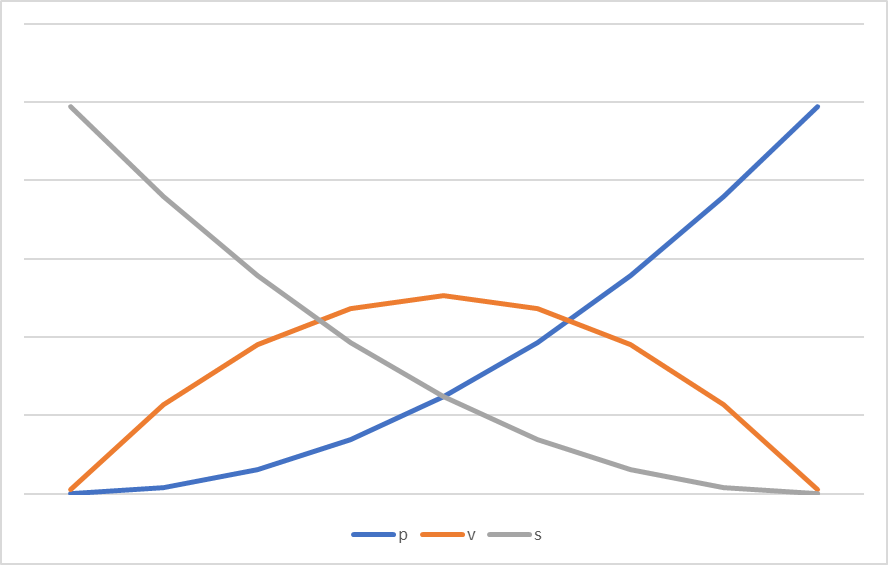
\includegraphics[width=0.45\textwidth]{figuras/roca.png}   
\caption{Relación entre s, v y p en el patrón roca\cite{propiaExcel}}
\label{fig:roca}
\end{figure}


\begin{itemize}
\item Probabilidad en caso de mejor jugada: [p,v,s]=[0,0.01,0.99] 
\item Probabilidad en caso de peor jugada: [p,v,s]=[0.99,0.01,0]
\end{itemize}

\subsubsection{Preflop}

En este caso, las parábolas de p y s son las siguientes:
\begin{itemize}
\item $p=0.01546875*esc^2 $
\item $s=0.01546875*(esc-8)^2$
\end{itemize}

Siendo esc $\in$[0,8], correspondiendo 0=Grupo 1 y 8=Sin grupo.

\begin{longtable}[c]{|c|c|c|c|}
\hline
\rowcolor{lightgray}Grupo Sklansky - Malmuth & \%pasar & \%ver & \%subir \\ \hline
Grupo 1 & 0 & 0,01 & 0,99 \\ \hline
Grupo 2 & 0,01546875 & 0,2265625 & 0,75796875 \\ \hline
Grupo 3 & 0,061875 & 0,38125 & 0,556875 \\ \hline
Grupo 4 & 0,13921875 & 0,4740625 & 0,38671875 \\ \hline
Grupo 5 & 0,2475 & 0,505 & 0,2475 \\ \hline
Grupo 6 & 0,38671875 & 0,4740625 & 0,13921875 \\ \hline
Grupo 7 & 0,556875 & 0,38125 & 0,061875 \\ \hline
Grupo 8 & 0,75796875 & 0,2265625 & 0,01546875 \\ \hline
Sin Grupo & 0,99 & 0,01 & 0 \\ \hline
\end{longtable}
\subsubsection{Postflop}

En este caso, las parábolas de p y s son las siguientes:
\begin{itemize}
\item $p=0.01222222*esc^2 $
\item $s=0.01222222*(esc-9)2$
\end{itemize}

Siendo esc $\in$[0,9], siendo cada uno de los escalones el valor entero de la jugada obtenida.

\begin{longtable}[c]{|c|c|c|c|}
\hline
\rowcolor{lightgray}Jugada & \%pasar & \%ver & \%subir \\ \hline
Escalera real & 0 & 0,01 & 0,99 \\ \hline
Escalera de Color & 0,01222222 & 0,20555556 & 0,78222222 \\ \hline
Pˇker & 0,04888889 & 0,35222222 & 0,59888889 \\ \hline
Full & 0,11 & 0,45 & 0,44 \\ \hline
Color & 0,19555556 & 0,49888889 & 0,30555556 \\ \hline
Escalera & 0,30555556 & 0,49888889 & 0,19555556 \\ \hline
Trio & 0,44 & 0,45 & 0,11 \\ \hline
Doble pareja & 0,59888889 & 0,35222222 & 0,04888889 \\ \hline
Pareja & 0,78222222 & 0,20555556 & 0,01222222 \\ \hline
Carta alta & 0,99 & 0,01 & 0 \\ \hline
\end{longtable}

\subsection{Calling Station}

El comportamiento de este patrón va a ser bastante similar al de maniaco, únicamente priorizando la probabilidad de ver la apuesta por encima de subir. También se tendrá un comportamiento lineal, aunque en este caso, la probabilidad que estará en función de las otras dos es la de pasar, ya que se le quiere dar más importancia a Ver.

En este caso, se van a definir los siguientes valores:
\begin{itemize}
\item Probabilidad en caso de mejor jugada: [p,v,s]=[0,0.85,0.15] 
\item Decremento de s: -0.0125 x escalón.
\item  Decremento de v: -0.025 x escalón.
\item El valor de p=1-(v+s) en este caso significa que p irá en incremento por escalón de +0.0375 x escalón.
\end{itemize}

\subsubsection{Preflop}
\begin{longtable}[c]{|c|c|c|c|}
\hline
\rowcolor{lightgray}Grupo Sklansky - Malmuth & \%pasar & \%ver & \%subir \\ \hline
Grupo 1 & 0 & 0,85 & 0,15 \\ \hline
Grupo 2 & 0,0375 & 0,825 & 0,1375 \\ \hline
Grupo 3 & 0,075 & 0,8 & 0,125 \\ \hline
Grupo 4 & 0,1125 & 0,775 & 0,1125 \\ \hline
Grupo 5 & 0,15 & 0,75 & 0,1 \\ \hline
Grupo 6 & 0,1875 & 0,725 & 0,0875 \\ \hline
Grupo 7 & 0,225 & 0,7 & 0,075 \\ \hline
Grupo 8 & 0,2625 & 0,675 & 0,0625 \\ \hline
Sin Grupo & 0,3 & 0,65 & 0,05 \\ \hline

\end{longtable}
\subsubsection{Postflop}

\begin{longtable}[c]{|c|c|c|c|}
\hline
\rowcolor{lightgray}Jugada & \%pasar & \%ver & \%subir \\ \hline
Escalera real & 0 & 0,85 & 0,15 \\ \hline
Escalera de Color & 0,0375 & 0,825 & 0,1375 \\ \hline
Pˇker & 0,075 & 0,8 & 0,125 \\ \hline
Full & 0,1125 & 0,775 & 0,1125 \\ \hline
Color & 0,15 & 0,75 & 0,1 \\ \hline
Escalera & 0,1875 & 0,725 & 0,0875 \\ \hline
Trio & 0,225 & 0,7 & 0,075 \\ \hline
Doble pareja & 0,2625 & 0,675 & 0,0625 \\ \hline
Pareja & 0,3 & 0,65 & 0,05 \\ \hline
Carta alta & 0,3375 & 0,625 & 0,0375 \\ \hline
\end{longtable}

\subsection{Cálculos para la formula de Bayes}
\label{sec:calcbayes}

En este apartado se va a desarrollar como se ha pasado de estos modelos a cifras para usar la fórmula de Bayes en el algoritmo óptimo.
Recordando el apartado \ref{sec:bayes}, son necesarios 4 datos para aplicar la fórmula:

\begin{itemize}
\item $p(A | B)$
\item  $p(A|\tilde{B})$
\item  $p(B)$
\item $p(\tilde{B})$
\end{itemize}

Teniendo en cuenta que A hace referencia al evento de \textit{ha tomado la acción} y B el evento de \textit{es un patrón concreto}, se puede reescribir de esta manera:
\begin{itemize}
\item $p(A | B)$: probabilidad de que, dado el patrón, haya tomado la acción
\item $ p(A|\tilde{B})$:  probabilidad de que, siendo un patron distinto al dado, haya tomado la acción
\item  $p(B)$: probabilidad de que sea ese patrón.
\item $p(tilde{B})$:probabilidad de queno  sea ese patrón.
\end{itemize}
La probabilidad de que sea o no sea el patrón irá variando en función de la toma de decisiones, puesto que será el resultado de la propia fórmula de Bayes (siendo el valor inicial 33\%). Por tanto, es necesario calcular $ p(A | B)$ y $p(A|\tilde{B})$.

Durante el preflop, ambos dependen del valor de la mano, se procede a analizar en qué casos ocurre cada acción. Hay que tener en cuenta que durante el preflop, las posibilidades son $\binom{52}{2}=1326$ posibles manos.


\begin{longtable}[c]{|c|c|c|c|}
\hline
\rowcolor{lightgray}Grupo Sklansky - Malmuth & Número de Manos del grupo & \% \\ \hline
Grupo 1 & 28 & 2,11\% \\ \hline
Grupo 2 & 30 & 2,26\% \\ \hline
Grupo 3 & 34 & 2,56\% \\ \hline
Grupo 4 & 46 & 3,47\% \\ \hline
Grupo 5 & 98 & 7,39\% \\ \hline
Grupo 6 & 108 & 8,14\% \\ \hline
Grupo 7 & 62 & 4,68\% \\ \hline
Grupo 8 & 154 & 11,61\% \\ \hline
Sin Grupo & 766 & 57,77\% \\ \hline
\end{longtable}

De esta manera, se ha realizado la suma ponderada con estos pesos a cada una de las acciones de los tres patrones durante el preflop, para determinar la probabilidad de que uno de esos patrones tome una acción.

\begin{longtable}[c]{|c|c|c|c|}
\hline
\rowcolor{lightgray}\multicolumn{4}{|c|}{p(A \textbar B) durante el preflop} \\ \hline
Patron & P(pasar) & P(ver) & P(subir) \\ \hline
Maniaco & 0,16489442 & 0,21489442 & 0,62021116 \\ \hline
Roca & 0,74252333 & 0,15740809 & 0,10006858 \\ \hline
Calling Station & 0,24734163 & 0,68510558 & 0,06755279 \\ \hline
\end{longtable}

El caso de las rondas posteriores al Preflop, el procedimiento es idéntico. En este caso, el número de jugadas posibles es $\binom{52}{5}=$2.598.960 combinaciones.

\begin{longtable}[c]{|c|c|c|c|}
\hline
\rowcolor{lightgray}Jugada & Combinaciones posibles & \% \\ \hline
Escalera real & 4 & 0,00\% \\ \hline
Escalera de Color & 36 & 0,00\% \\ \hline
Pˇker & 624 & 0,02\% \\ \hline
Full & 3744 & 0,14\% \\ \hline
Color & 5108 & 0,20\% \\ \hline
Escalera & 10200 & 0,39\% \\ \hline
Trio & 54912 & 2,11\% \\ \hline
Doble pareja & 123552 & 4,75\% \\ \hline
Pareja & 1098240 & 42,26\% \\ \hline
Carta alta & 1302540 & 50,12\% \\ \hline
\end{longtable}

Con estos pesos, se puede hacer la suma ponderada, tal y como se ha hecho en el caso anterior.

Haciendo esta suma ponderada de cada uno de los patrones, se tienen los siguientes valores de $p(A | B)$ en rondas posteriores a preflop.


\begin{longtable}[c]{|c|c|c|c|}
\hline
\rowcolor{lightgray}\multicolumn{4}{|c|}{p(A | B) después del preflop} \\ \hline
Patron & P(pasar) & P(ver) & P(subir) \\ \hline
Maniaco & 0,20957483 & 0,25957483 & 0,53085034 \\ \hline
Roca & 0,86622952 & 0,12179945 & 0,01197102 \\ \hline
Calling Station & 0,31436224 & 0,64042517 & 0,04521259 \\ \hline
\end{longtable}

Ya habiendo calculado los posibles valores de$ p(A | B)$, se pueden calcular los valores de$ p(A | \tilde{B})$.
Yendo a la definición de$ p(A | \tilde{B})$, se encuentra que es el caso en que sin ser el algoritmo, se haya tomado esa acción. En otras palabras, se puede definer $ p(A | \tilde{B})$como que cualquiera de los otros algoritmos haya tomado esa acción. Teniendo esto en consideración, y teniendo en cuenta que solo hay 3 patrones, se puede definir como:

\[ 
p(A | \tilde{B})= p(A | x \cup y) = p(A | x) \cup p(A | y) =  p(A | x) + p(A | y) 
\]

Siendo x e y los otros patrones distintos de B.
De esta manera, se tienen todos los valores para el cálculo del teorema de Bayes.

\section {Desarrollo del algoritmo óptimo.}
\label{sec:optimus}

Este algoritmo tiene como objetivo calcular las probabilidades de tener una mano más fuerte que la del oponente, una mano similar a la del oponente o una mano peor que la del oponente; y con esa probabilidad, tomar una de las tres posibles acciones: ver la apuesta, de subir la apuesta o de pasar la apuesta. Para ello, se deben de tener en consideración siempre las cartas de las que se tiene información:

\begin{itemize}
\item \textbf{Información común para todas las fases de la ronda}

Durante cada fase de la ronda, siempre se van a tener los siguientes datos:
\begin{itemize}
\item La mano conocida: dos cartas, cada una con un número y un palo, que son dos cartas conocidas.
\item La mano del otro jugador: dos cartas, al igual que la propia mano, pero en este caso son cartas que van a ser desconocidas siempre hasta el final de la ronda. 
\item Cada carta es única, es decir, una carta no puede aparecer dos veces
\end{itemize} 
Con estos 3 datos, se puede apreciar que se tiene una incógnita que se debe suponer de cara a calcular las probabilidades arriba mencionadas, pero el tercer dato (la unicidad de las cartas) nos permite suponer cada una de las posibles manos del oponente y, con eso, poder calcular las probabilidades.

\item\textbf{Tablas de probabilidades: tabla de pesos relativos y tabla de probabilidad de acción del oponente}

Para todo el funcionamiento del algoritmo se va a partir de dos tablas: una tabla que va a recoger la probabilidad relativa de que el oponente tenga una mano y una segunda tabla que recoja la probabilidad de cada mano del oponente de tomar una decisión u otra.
La tabla de pesos relativos recoge todas las posibles combinaciones de cartas y un valor numérico, al que se denomina Peso relativo (P$_r$), que puede tener valores entre 0 y 1. Este valor indica cómo de probable es que el oponente tenga una mano y otra y se irá actualizando con la decisión que tome el oponente.
La tabla de pesos relativos inicialmente tendrá estos valores.


\begin{longtable}[c]{|c|c|c|c|c|c|c|c|c|c|c|c|c|c|c|c|c|}
\hline
& 11 & 12 & 13 & 14 & 21 & 22 & 23 & 24 & 31 & 32 & 33 & 34 & 41 & 42 & 43 & 44 \\ \hline
1414 & 0 & 1 & 1 & 1 & 0 & 0 & 1 & 1 & 0 & 0 & 0 & 1 & 0 & 0 & 0 & 0 \\ \hline
1313 & 0 & 1 & 1 & 1 & 0 & 0 & 1 & 1 & 0 & 0 & 0 & 1 & 0 & 0 & 0 & 0 \\ \hline
1212 & 0 & 1 & 1 & 1 & 0 & 0 & 1 & 1 & 0 & 0 & 0 & 1 & 0 & 0 & 0 & 0 \\ \hline
1111 & 0 & 1 & 1 & 1 & 0 & 0 & 1 & 1 & 0 & 0 & 0 & 1 & 0 & 0 & 0 & 0 \\ \hline
1010 & 0 & 1 & 1 & 1 & 0 & 0 & 1 & 1 & 0 & 0 & 0 & 1 & 0 & 0 & 0 & 0 \\ \hline
909 & 0 & 1 & 1 & 1 & 0 & 0 & 1 & 1 & 0 & 0 & 0 & 1 & 0 & 0 & 0 & 0 \\ \hline
808 & 0 & 1 & 1 & 1 & 0 & 0 & 1 & 1 & 0 & 0 & 0 & 1 & 0 & 0 & 0 & 0 \\ \hline
707 & 0 & 1 & 1 & 1 & 0 & 0 & 1 & 1 & 0 & 0 & 0 & 1 & 0 & 0 & 0 & 0 \\ \hline
606 & 0 & 1 & 1 & 1 & 0 & 0 & 1 & 1 & 0 & 0 & 0 & 1 & 0 & 0 & 0 & 0 \\ \hline
505 & 0 & 1 & 1 & 1 & 0 & 0 & 1 & 1 & 0 & 0 & 0 & 1 & 0 & 0 & 0 & 0 \\ \hline
404 & 0 & 1 & 1 & 1 & 0 & 0 & 1 & 1 & 0 & 0 & 0 & 1 & 0 & 0 & 0 & 0 \\ \hline
303 & 0 & 1 & 1 & 1 & 0 & 0 & 1 & 1 & 0 & 0 & 0 & 1 & 0 & 0 & 0 & 0 \\ \hline
202 & 0 & 1 & 1 & 1 & 0 & 0 & 1 & 1 & 0 & 0 & 0 & 1 & 0 & 0 & 0 & 0 \\ \hline
1413 & 1 & 1 & 1 & 1 & 1 & 1 & 1 & 1 & 1 & 1 & 1 & 1 & 1 & 1 & 1 & 1 \\ \hline
1412 & 1 & 1 & 1 & 1 & 1 & 1 & 1 & 1 & 1 & 1 & 1 & 1 & 1 & 1 & 1 & 1 \\ \hline
1411 & 1 & 1 & 1 & 1 & 1 & 1 & 1 & 1 & 1 & 1 & 1 & 1 & 1 & 1 & 1 & 1 \\ \hline
1410 & 1 & 1 & 1 & 1 & 1 & 1 & 1 & 1 & 1 & 1 & 1 & 1 & 1 & 1 & 1 & 1 \\ \hline
1409 & 1 & 1 & 1 & 1 & 1 & 1 & 1 & 1 & 1 & 1 & 1 & 1 & 1 & 1 & 1 & 1 \\ \hline
1408 & 1 & 1 & 1 & 1 & 1 & 1 & 1 & 1 & 1 & 1 & 1 & 1 & 1 & 1 & 1 & 1 \\ \hline
1407 & 1 & 1 & 1 & 1 & 1 & 1 & 1 & 1 & 1 & 1 & 1 & 1 & 1 & 1 & 1 & 1 \\ \hline
1406 & 1 & 1 & 1 & 1 & 1 & 1 & 1 & 1 & 1 & 1 & 1 & 1 & 1 & 1 & 1 & 1 \\ \hline
1405 & 1 & 1 & 1 & 1 & 1 & 1 & 1 & 1 & 1 & 1 & 1 & 1 & 1 & 1 & 1 & 1 \\ \hline
1404 & 1 & 1 & 1 & 1 & 1 & 1 & 1 & 1 & 1 & 1 & 1 & 1 & 1 & 1 & 1 & 1 \\ \hline
1403 & 1 & 1 & 1 & 1 & 1 & 1 & 1 & 1 & 1 & 1 & 1 & 1 & 1 & 1 & 1 & 1 \\ \hline
1402 & 1 & 1 & 1 & 1 & 1 & 1 & 1 & 1 & 1 & 1 & 1 & 1 & 1 & 1 & 1 & 1 \\ \hline
1312 & 1 & 1 & 1 & 1 & 1 & 1 & 1 & 1 & 1 & 1 & 1 & 1 & 1 & 1 & 1 & 1 \\ \hline
1311 & 1 & 1 & 1 & 1 & 1 & 1 & 1 & 1 & 1 & 1 & 1 & 1 & 1 & 1 & 1 & 1 \\ \hline
1310 & 1 & 1 & 1 & 1 & 1 & 1 & 1 & 1 & 1 & 1 & 1 & 1 & 1 & 1 & 1 & 1 \\ \hline
1309 & 1 & 1 & 1 & 1 & 1 & 1 & 1 & 1 & 1 & 1 & 1 & 1 & 1 & 1 & 1 & 1 \\ \hline
1308 & 1 & 1 & 1 & 1 & 1 & 1 & 1 & 1 & 1 & 1 & 1 & 1 & 1 & 1 & 1 & 1 \\ \hline
1307 & 1 & 1 & 1 & 1 & 1 & 1 & 1 & 1 & 1 & 1 & 1 & 1 & 1 & 1 & 1 & 1 \\ \hline
1306 & 1 & 1 & 1 & 1 & 1 & 1 & 1 & 1 & 1 & 1 & 1 & 1 & 1 & 1 & 1 & 1 \\ \hline
1305 & 1 & 1 & 1 & 1 & 1 & 1 & 1 & 1 & 1 & 1 & 1 & 1 & 1 & 1 & 1 & 1 \\ \hline
1304 & 1 & 1 & 1 & 1 & 1 & 1 & 1 & 1 & 1 & 1 & 1 & 1 & 1 & 1 & 1 & 1 \\ \hline
1303 & 1 & 1 & 1 & 1 & 1 & 1 & 1 & 1 & 1 & 1 & 1 & 1 & 1 & 1 & 1 & 1 \\ \hline
1302 & 1 & 1 & 1 & 1 & 1 & 1 & 1 & 1 & 1 & 1 & 1 & 1 & 1 & 1 & 1 & 1 \\ \hline
1211 & 1 & 1 & 1 & 1 & 1 & 1 & 1 & 1 & 1 & 1 & 1 & 1 & 1 & 1 & 1 & 1 \\ \hline
1210 & 1 & 1 & 1 & 1 & 1 & 1 & 1 & 1 & 1 & 1 & 1 & 1 & 1 & 1 & 1 & 1 \\ \hline
1209 & 1 & 1 & 1 & 1 & 1 & 1 & 1 & 1 & 1 & 1 & 1 & 1 & 1 & 1 & 1 & 1 \\ \hline
1208 & 1 & 1 & 1 & 1 & 1 & 1 & 1 & 1 & 1 & 1 & 1 & 1 & 1 & 1 & 1 & 1 \\ \hline
1207 & 1 & 1 & 1 & 1 & 1 & 1 & 1 & 1 & 1 & 1 & 1 & 1 & 1 & 1 & 1 & 1 \\ \hline
1206 & 1 & 1 & 1 & 1 & 1 & 1 & 1 & 1 & 1 & 1 & 1 & 1 & 1 & 1 & 1 & 1 \\ \hline
1205 & 1 & 1 & 1 & 1 & 1 & 1 & 1 & 1 & 1 & 1 & 1 & 1 & 1 & 1 & 1 & 1 \\ \hline
1204 & 1 & 1 & 1 & 1 & 1 & 1 & 1 & 1 & 1 & 1 & 1 & 1 & 1 & 1 & 1 & 1 \\ \hline
1203 & 1 & 1 & 1 & 1 & 1 & 1 & 1 & 1 & 1 & 1 & 1 & 1 & 1 & 1 & 1 & 1 \\ \hline
1202 & 1 & 1 & 1 & 1 & 1 & 1 & 1 & 1 & 1 & 1 & 1 & 1 & 1 & 1 & 1 & 1 \\ \hline
1110 & 1 & 1 & 1 & 1 & 1 & 1 & 1 & 1 & 1 & 1 & 1 & 1 & 1 & 1 & 1 & 1 \\ \hline
1109 & 1 & 1 & 1 & 1 & 1 & 1 & 1 & 1 & 1 & 1 & 1 & 1 & 1 & 1 & 1 & 1 \\ \hline
1108 & 1 & 1 & 1 & 1 & 1 & 1 & 1 & 1 & 1 & 1 & 1 & 1 & 1 & 1 & 1 & 1 \\ \hline
1107 & 1 & 1 & 1 & 1 & 1 & 1 & 1 & 1 & 1 & 1 & 1 & 1 & 1 & 1 & 1 & 1 \\ \hline
1106 & 1 & 1 & 1 & 1 & 1 & 1 & 1 & 1 & 1 & 1 & 1 & 1 & 1 & 1 & 1 & 1 \\ \hline
1105 & 1 & 1 & 1 & 1 & 1 & 1 & 1 & 1 & 1 & 1 & 1 & 1 & 1 & 1 & 1 & 1 \\ \hline
1104 & 1 & 1 & 1 & 1 & 1 & 1 & 1 & 1 & 1 & 1 & 1 & 1 & 1 & 1 & 1 & 1 \\ \hline
1103 & 1 & 1 & 1 & 1 & 1 & 1 & 1 & 1 & 1 & 1 & 1 & 1 & 1 & 1 & 1 & 1 \\ \hline
1102 & 1 & 1 & 1 & 1 & 1 & 1 & 1 & 1 & 1 & 1 & 1 & 1 & 1 & 1 & 1 & 1 \\ \hline
1009 & 1 & 1 & 1 & 1 & 1 & 1 & 1 & 1 & 1 & 1 & 1 & 1 & 1 & 1 & 1 & 1 \\ \hline
1008 & 1 & 1 & 1 & 1 & 1 & 1 & 1 & 1 & 1 & 1 & 1 & 1 & 1 & 1 & 1 & 1 \\ \hline
1007 & 1 & 1 & 1 & 1 & 1 & 1 & 1 & 1 & 1 & 1 & 1 & 1 & 1 & 1 & 1 & 1 \\ \hline
1006 & 1 & 1 & 1 & 1 & 1 & 1 & 1 & 1 & 1 & 1 & 1 & 1 & 1 & 1 & 1 & 1 \\ \hline
1005 & 1 & 1 & 1 & 1 & 1 & 1 & 1 & 1 & 1 & 1 & 1 & 1 & 1 & 1 & 1 & 1 \\ \hline
1004 & 1 & 1 & 1 & 1 & 1 & 1 & 1 & 1 & 1 & 1 & 1 & 1 & 1 & 1 & 1 & 1 \\ \hline
1003 & 1 & 1 & 1 & 1 & 1 & 1 & 1 & 1 & 1 & 1 & 1 & 1 & 1 & 1 & 1 & 1 \\ \hline
1002 & 1 & 1 & 1 & 1 & 1 & 1 & 1 & 1 & 1 & 1 & 1 & 1 & 1 & 1 & 1 & 1 \\ \hline
908 & 1 & 1 & 1 & 1 & 1 & 1 & 1 & 1 & 1 & 1 & 1 & 1 & 1 & 1 & 1 & 1 \\ \hline
907 & 1 & 1 & 1 & 1 & 1 & 1 & 1 & 1 & 1 & 1 & 1 & 1 & 1 & 1 & 1 & 1 \\ \hline
906 & 1 & 1 & 1 & 1 & 1 & 1 & 1 & 1 & 1 & 1 & 1 & 1 & 1 & 1 & 1 & 1 \\ \hline
905 & 1 & 1 & 1 & 1 & 1 & 1 & 1 & 1 & 1 & 1 & 1 & 1 & 1 & 1 & 1 & 1 \\ \hline
904 & 1 & 1 & 1 & 1 & 1 & 1 & 1 & 1 & 1 & 1 & 1 & 1 & 1 & 1 & 1 & 1 \\ \hline
903 & 1 & 1 & 1 & 1 & 1 & 1 & 1 & 1 & 1 & 1 & 1 & 1 & 1 & 1 & 1 & 1 \\ \hline
902 & 1 & 1 & 1 & 1 & 1 & 1 & 1 & 1 & 1 & 1 & 1 & 1 & 1 & 1 & 1 & 1 \\ \hline
807 & 1 & 1 & 1 & 1 & 1 & 1 & 1 & 1 & 1 & 1 & 1 & 1 & 1 & 1 & 1 & 1 \\ \hline
806 & 1 & 1 & 1 & 1 & 1 & 1 & 1 & 1 & 1 & 1 & 1 & 1 & 1 & 1 & 1 & 1 \\ \hline
805 & 1 & 1 & 1 & 1 & 1 & 1 & 1 & 1 & 1 & 1 & 1 & 1 & 1 & 1 & 1 & 1 \\ \hline
804 & 1 & 1 & 1 & 1 & 1 & 1 & 1 & 1 & 1 & 1 & 1 & 1 & 1 & 1 & 1 & 1 \\ \hline
803 & 1 & 1 & 1 & 1 & 1 & 1 & 1 & 1 & 1 & 1 & 1 & 1 & 1 & 1 & 1 & 1 \\ \hline
802 & 1 & 1 & 1 & 1 & 1 & 1 & 1 & 1 & 1 & 1 & 1 & 1 & 1 & 1 & 1 & 1 \\ \hline
706 & 1 & 1 & 1 & 1 & 1 & 1 & 1 & 1 & 1 & 1 & 1 & 1 & 1 & 1 & 1 & 1 \\ \hline
705 & 1 & 1 & 1 & 1 & 1 & 1 & 1 & 1 & 1 & 1 & 1 & 1 & 1 & 1 & 1 & 1 \\ \hline
704 & 1 & 1 & 1 & 1 & 1 & 1 & 1 & 1 & 1 & 1 & 1 & 1 & 1 & 1 & 1 & 1 \\ \hline
703 & 1 & 1 & 1 & 1 & 1 & 1 & 1 & 1 & 1 & 1 & 1 & 1 & 1 & 1 & 1 & 1 \\ \hline
702 & 1 & 1 & 1 & 1 & 1 & 1 & 1 & 1 & 1 & 1 & 1 & 1 & 1 & 1 & 1 & 1 \\ \hline
605 & 1 & 1 & 1 & 1 & 1 & 1 & 1 & 1 & 1 & 1 & 1 & 1 & 1 & 1 & 1 & 1 \\ \hline
604 & 1 & 1 & 1 & 1 & 1 & 1 & 1 & 1 & 1 & 1 & 1 & 1 & 1 & 1 & 1 & 1 \\ \hline
603 & 1 & 1 & 1 & 1 & 1 & 1 & 1 & 1 & 1 & 1 & 1 & 1 & 1 & 1 & 1 & 1 \\ \hline
602 & 1 & 1 & 1 & 1 & 1 & 1 & 1 & 1 & 1 & 1 & 1 & 1 & 1 & 1 & 1 & 1 \\ \hline
504 & 1 & 1 & 1 & 1 & 1 & 1 & 1 & 1 & 1 & 1 & 1 & 1 & 1 & 1 & 1 & 1 \\ \hline
503 & 1 & 1 & 1 & 1 & 1 & 1 & 1 & 1 & 1 & 1 & 1 & 1 & 1 & 1 & 1 & 1 \\ \hline
502 & 1 & 1 & 1 & 1 & 1 & 1 & 1 & 1 & 1 & 1 & 1 & 1 & 1 & 1 & 1 & 1 \\ \hline
403 & 1 & 1 & 1 & 1 & 1 & 1 & 1 & 1 & 1 & 1 & 1 & 1 & 1 & 1 & 1 & 1 \\ \hline
402 & 1 & 1 & 1 & 1 & 1 & 1 & 1 & 1 & 1 & 1 & 1 & 1 & 1 & 1 & 1 & 1 \\ \hline
302 & 1 & 1 & 1 & 1 & 1 & 1 & 1 & 1 & 1 & 1 & 1 & 1 & 1 & 1 & 1 & 1 \\ \hline
\end{longtable}

Representando cada fila una combinación de dos cartas y cada columna el palo (T= tréboles, P= picas, D=Diamantes y C=Corazones) de cada una de las cartas. Por ejemplo, si se toma el valor de la fila 807 y la columna CD, ese Peso relativo corresponde a la probabilidad de que el oponente tenga un 8 de corazones y un 7 de diamantes en función de sus acciones a lo largo de la partida.
Como se puede observar, hay varias combinaciones que siempre tendrán una probabilidad de 0. Estas combinaciones ocurren únicamente en las parejas ya que:
\begin{itemize} 
\item Al ser las cartas únicas, no puede haber dos cartas iguales. Por tanto, una pareja de dos cartas del mismo palo (por ejemplo, tener dos 9 de diamantes) es imposible. Por tanto, estos casos siempre tendrán probabilidad de 0.
\item Al ser parejas, el orden de las cartas no influye. Es decir, tener un As de diamantes y un As de picas es lo mismo que tener un As de picas y un As de diamantes. Por esta razón, a las posibilidades repetidas, se les ha dado valor 0 para evitar valores duplicados.
\end{itemize} 
A pesar de ser combinaciones imposibles de conseguir, se ha decidido mantenerlas por comodidad, ya que al mantenerlas se puede crear una matriz con todas las posibilidades. En caso de eliminarlas, habría que hacer dos matrices para recoger esos datos: una para las parejas y otra para las combinaciones de cartas que no sean parejas, dificultando el cálculo matemático.
También cada vez que una carta sea conocida, todas las combinaciones posibles con esa carta se convertirán en 0.
Para actualizar estos valores a lo largo de la partida, se tiene la segunda tabla, la denominada tabla de probabilidad triple de acción del oponente, o simplemente tabla de probabilidad triple de acción. Por cada jugador distinto del algoritmo, sería necesaria una tabla independiente, pero ya que solo hay únicamente dos jugadores, esto se simplifica a una única tabla.
Antes de hablar de la tabla, se va a explicar el concepto de probabilidad triple de acción del oponente. La probabilidad triple de acción del oponente es un conjunto de tres valores entre 0 y 1 {p, v, s} que representan cómo de probable es que el adversario tome una de las tres posibles acciones (pasar (p), ver (v) y subir (s)) desde el punto de vista del algoritmo. En otras palabras, es un conjunto de tres números que representa la probabilidad de que ocurra el evento de pasar la apuesta, el evento de ver la apuesta o el evento de subir la apuesta para cada mano.
Como estoy hablando de probabilidades, y sabiendo que siempre que ocurrir uno de los tres eventos, se cumple que $ p+v+s=1$.
La tabla de probabilidad triple de acción recoge la probabilidad triple de acción para cada combinación de cartas del oponente. Estas probabilidades serán
La tabla tendrá un aspecto como este para cada combinación de cartas:


\begin{longtable}[c]{|c|c|c|c|}
\hline
 & \%Pasar & \%Ver & \%Subir \\ \hline
$N_1P_1N_2P_2$ & p & v & S \\ \hline
\end{longtable}

Siendo $ N_1$ y $P_1$el número y palo de la primera carta y $N_2$ y $P_2$ el número y palo de la segunda

Dado que estos valores son probabilidades de acción, estos valores cambiarán con el paso de las rondas.
Previamente se ha mencionado que los valores de la tabla de pesos relativos se actualizarían con las acciones del oponente y los valores de la tabla de probabilidad de acción del oponente. En función de la acción del oponente, se multiplica el valor de la tabla de la tabla de pesos relativos para esa combinación por el valor de la acción elegida de la tabla de probabilidad de acción del oponente que tenga esa mano.
Se pone un ejemplo:
Si se tiene los siguientes pesos en la tabla de pesos relativos:
\[
P_r \{10\clubsuit 7\spadesuit\} = 0,7
\]
\[
P_r\{\textcolor{red}{09\vardiamondsuit 03\varheartsuit}\} = 0,3
\]
\[
P_r \{\textcolor{red}{A\vardiamondsuit} Q\spadesuit\} = 0,64
\]
Y las siguientes probabilidades triples de acción:
\[
PtA \{10\clubsuit 7\spadesuit\} = \{0,24; 0,61; 0,15\}
\]
\[
PtA \{\textcolor{red}{09\vardiamondsuit 03\varheartsuit}\} = \{0,61; 0,3; 0,09\}
\]
\[
PtA \{\textcolor{red}{A\vardiamondsuit} Q\spadesuit\} = \{0,03; 0,28; 0,69\}
\]
Si el oponente ve la apuesta, los nuevos valores de los pesos en la tabla serían:
\[
P_r \{10\clubsuit 7\spadesuit\}  = 0,7*0,61=0,427
\]
\[
P_r\{\textcolor{red}{09\vardiamondsuit 03\varheartsuit}\} = 0,3*0,3 = 0,09
\]
\[
P_r \{\textcolor{red}{A\vardiamondsuit} Q\spadesuit\} = 0,64*0,28 = 0,1792
\]
Como se puede observar, en caso de ver la apuesta, la combinación más probable de las tres consideradas sería $\{10\clubsuit 7\spadesuit\}$ y la menos probable sería $\{\textcolor{red}{09\vardiamondsuit 03\varheartsuit}\}$. También se aprecia que la probabilidad de que sea  $\{\textcolor{red}{A\vardiamondsuit} Q\spadesuit\}$ también ha bajado, pues con esa mano lo más probable hubiera sido subir la apuesta.
Una vez explicado estas bases, se pasa a explicar el funcionamiento del algoritmo.
Para empezar, se tiene considerar que la información conocida en las fases varía:
\begin{itemize}
\item Durante el preflop, únicamente se tiene la mano 
\item Durante el flop se tiene la propia mano y 3 cartas comunes
\item Durante el turn, se tiene la propia mano y 4 cartas comunes
\item Durante el river, se tiene la propia mano y las 5 cartas comunes.
\end{itemize}
Por tanto, el comportamiento del algoritmo  se tiene que adaptar para que pueda reflejar esta variación de información.
Para ello, se procede a dividir el algoritmo en tres “partes”, cada una con un funcionamiento particular:
\begin{enumerate}
\item Cuando no se tiene información de las cartas de la mesa. (Preflop)
\item Cuando hay información de cartas de la mesa y aún quedan cartas por salir (Flop y Turn)
\item Cuando ya está toda la información de las cartas de la mesa (River)
\end{enumerate}

\end{itemize} 

El funcionamiento general de la actualización es calcular los factores de la mano propia, calcular la probabilidad triple de acción del algoritmo actualizar la tabla de triple probabilidad y, por ultimo,  actualizar la tabla de pesos del oponente con la acción tomada por el oponente y la tabla de triple probabilidad de acción del oponente. 

\subsection{Preflop}

En esta fase, solo se dispone de 2 cartas de información conocida, por lo tanto restan 50 cartas posibles, de las cuales cualquier combinación de esas 2 cartas podrían ser las que quedan en la mano del oponente, lo que significa un total de $\binom{50}{2} = 1225 $combinaciones posibles.
Otra de las peculiaridades de esta fase es que, puede que no haya habido ningún tipo de apuesta por parte del oponente al comienzo de esta apuesta, por lo que los pesos podrían ser iguales uno a otro.
Como ya se ha comentado en el apartado \ref{sec:chen} hablado previamente, la fuerza de una mano en el preflop se ha determinado mediante la fórmula de Chen. Es cierto que esta fórmula tiene sus limitaciones, pero como un indicador base nos sirve de guía de cara a automatizar este proceso.
Tal y como se mencionó en el apartado \ref{sec:chen}, Chen, según su experiencia, nos indicaba varias puntuaciones por las que se podría empezar a jugar una mano.\cite{krieger} Pero, en una partida de dos jugadores, no hay posiciones, ya que no hay jugadores intermedios entre un jugador y el Dealer. Pero partiendo de ese criterio, y del cruce con Sklansky-Malmuth (ver figura \ref{fig:sklansky},  se puede determinar qué manos ver, qué manos subir y qué manos desechar. 
Una de las cualidades que se busca  en el algoritmo es que sea imprevisible, por lo que se van a añadir porcentajes de acción, para que, aunque se tenga una acción predominante, no siempre sea preciso.
En función del valor de la fórmula de Chen, se establece esta valoración de triples probabilidades:


\begin{longtable}[c]{|c|c|c|c|}
\hline
\rowcolor{lightgray}Puntuación Chen & \%pasar & \%ver & \%subir \\ \hline
12-20 & 0 & 0,1 & 0,9 \\ \hline
10-11 & 0 & 0,25 & 0,75 \\ \hline
5*-9 & 0,25 & 0,65 & 0,1 \\ \hline
3,5-5** & 0,69 & 0,3 & 0,01 \\ \hline
Menor de 3,5 & 0,99 & 0,01 & 0 \\ \hline
\end{longtable}

Para esta valoraciones y asignar estos pesos,se han tomado en consideración los siguientes aspectos:
\begin{itemize}
\item Los pertenecientes al Grupo uno de Sklansky-Malmuth (12-20) son manos con las que son convenientes tomar la estrategia de subir la mano, por tanto, son manos que siempre se van a jugar. Además, son manos que, ante una subida, también son partidarias de resubir dicha subida.
\item Los pertenecientes al Grupo 2 (10-11) son manos con las que son convenientes tomar una estrategia agresiva pero no tanto como las del grupo anterior, por tanto, son manos que prácticamente siempre se van a jugar. Además, son manos que, ante una subida, también son partidarias de ver dicha subida, pero no de subirlas
\item Las manos pertenecientes a los grupos 3 al 6 (5*-9) son las manos que, según Chen, son manos jugables según la posición que se tenga. Por tanto, se puede asumir que son manos que suelen ver las apuestas, aunque ante resubidas, suelen pasar.  *Las manos de valor 5 incluidas aquí son únicamente las parejas (si bien la pareja de 5 es la única combinación de valor 5 según la fórmula de Chen que pertenece al grupo 6, considero que, dado que las otras parejas se pueden incluir aquí ya que son una jugada hecha y, además, al solo haber un oponente, no son tan fácil de superar como si hubiera más jugadores puesto que, a más jugadores, más posibilidades de que se forme una pareja con cualquiera de las cartas comunes.
\item Las manos pertenecientes a los grupos 7 y 8 (3,5-5**) son manos que son difíciles de ganar, pero aún se consideran con posibilidades según la clasificación de Sklansky-Malmuth. Tanto Chen como Krieger\cite{krieger} recomiendan que estas manos sean descartadas, por eso se le da un mayor peso a pasar que a ver. **Aquí no están incluidas las incluidas en el punto anterior, pero si están incluidas las combinaciones de AX de distinto palos siendo $X>9$ puesto que, aunque la fórmula de Chen les dé una valoración de 5, Malmuth-Sklansky las descarta como manos jugables. Se ha decidido incluirlas por un razonamiento similar al anterior punto: al haber un solo oponente esta combinación de cartas gana fuerza.
\item Manos por debajo de 3,5: son las combinaciones que están fuera de los grupos Sklansky-Malmuth, con la excepción mencionada en el punto anterior, por lo que son manos con muchas dificultades para ganar la jugada. Por ende, son manos prácticamente descartables.
\end{itemize}

De estos razonamientos se puede establecer una segunda tabla de probabilidad triple, ante la resubida en caso de que el oponente suba:

\begin{longtable}[c]{|c|c|c|c|}
\hline
\rowcolor{lightgray}Puntuación Chen & \%pasar & \%ver & \%subir \\ \hline
12-20 & 0 & 0,2 & 0,8 \\ \hline
10-11 & 0 & 0,8 & 0,2 \\ \hline
5*-9 & 0,85 & 0,1 & 0,05 \\ \hline
5 o menor & 0,99 & 0,01 & 0 \\ \hline
\end{longtable}


A medida que va avanzando la partida, se puede observar que se van perfilando las manos del oponente según sus acciones. 
Una vez obtenida la probabilidad de acción triple del algoritmo, es necesario ajustarla en función del algoritmo al que se enfrente. Para eso, se crea la función \textit{ajusteBayes}. Esta función calculará cual de los 3 patrones es el mas probable que sea y en función de a cual de los 3 sea el más probable según bayes (aplicando la fórmula del teorema de bayes a cada uno de los tres patrones), se ajustará la probabilidad para compensar la fortaleza de dicho patrón. En caso de que no se sepa identificar el patrón por cercanía de los patrones más probables mantendrá las probabilidades igual.

Independientemente de si no es capaz de identificar el patrón o no, almacenará estas tres probabilidades (la probabilidad de el oponente sea maniaco, sea Roca o sea Calling Station), almacenará los valores en un fichero para su reutilización en posteriores llamadas a la función.
\begin{verbatim}

ajusteBayes(triple, accion, ronda)
      [Maniaco,Roca, Calling Station] <- cargadeProbabilidades(ronda)
      PatronMasProbable<-comparaProbabilidades
      triple_actualizado<-ajuste(PatronMasProbable,accion,triple)
      return(triple_actualizado)
\end{verbatim}

El ajuste en cada ronda será en función del valor de la jugada y del patrón al que se enfrente, ya que cada uno de los patrones tienen debilidades, por lo que se modificarán los pesos en función de esas debilidades. 
Tras eso, es necesario actualizar la Tabla de Probabilidad de acción del oponente.
Para ello, se va a aplicar las tablas de probabilidades de acción de cada ronda para el algoritmo supuesto, creando la función \textit{CalculoProbabilidadAccion}.

\begin{verbatim}
CalculoProbabilidadAccion(mesa,mazo,tabla_triple,ronda)
      [Maniaco,Roca, Calling Station] <- cargadeProbabilidades(ronda)
      PatronMasProbable<-comparaProbabilidades
      valoresNuevosPatron <-cargadeValoresPatrones(ronda, Patron)
      para  cada  (ManoOp)
            {
            categoria<-ValorarJugada(ronda,ManoOp,mesa)
            tabla_triple[i]<-valoresNuevos[categoria]
            }
      return(tabla_triple)
\end{verbatim}

Dado que en esta ronda no hay cartas en Mesa, ese valor es 0.
Una vez actualizados los valores de acción y las tablas correspondientes, se continúa con la siguiente ronda de juego.

\subsection{Flop y Turn}
\label{sec:flopturn}

Se han agrupado ambas fases en este punto porque tienen una composición parecida: hay varias cartas comunes, pero aún quedan cartas por salir. Además, al haber al menos 5 cartas entre la mano y la mesa, la fórmula de Chen deja de ser efectiva pues ya hay jugadas. Ahora las jugadas siguen la puntuación mencionada previamente (0 a 9, siendo 0 carta más alta y 9 Escalera Real).

Lo primero que hay que hacer es actualizar la tabla de probabilidades con las cartas reveladas en la fase correspondiente (3 cartas en Flop y 1 en Turn), haciendo que todas las combinaciones de cartas que incluyan dichas cartas tengan probabilidad 0.

Despues, se puede empezar a valorar la situación con la información que se tiene.
En este caso, no se puede hacer un simple cálculo para determinar qué puede tener el oponente, puesto que hay muchas más variables posibles en lo que se refiere a las posibles combinaciones de mano.
Para poder automatizar esto, se va a tomar como base las ideas plasmadas en Algorithms and Assessment in Computer Póker , la tesis doctoral de Darse Billings de la universidad de Alberta\cite{doctor}. En la tesis, habla de distintas estrategias para cómo automatizar el juego de póker.
En dicha tesis, se define el valor de Fuerza de Mano (FM), que es la probabilidad de que una mano sea mejor que la del oponente, al igual que el Valor Potencial de la Mano (VPM), que es la fuerza potencial con las posteriores cartas.
Estas definiciones sirven de base para este proyecto, aunque se van a realizar modificaciones sobre eso para que se amolden a este algoritmo. Para empezar, se va a calcular cómo de buena es la mano con respecto a las posibles manos del oponente. Pero antes de eso, es necesario hacer una simplificación, de cara a ayudar a los cálculos: únicamente se van a tomar en consideración variaciones en la puntuación directa de la jugada, no en su desempate. Es decir, si cada jugador tiene una pareja, se van a considerar como “jugadas iguales”, aunque en la práctica esto no tenga que ser estrictamente cierto.
Con esto, se puede empezar a ver cómo de buena es esta mano, para eso se comprueba si, con cada combinación de dos cartas posibles del oponente su jugada es mejor, peor o igual que la del jugador.
\begin{verbatim}
CalcularFuerzaMano(valorjugadaJugador, Mesa)
      *Considerando cada una de las posibles manos del oponente*
      para cada (ManoOp):
            {
            valorjugadaOp <- calcularValorJugada(ManoO,Mesa);
            si valorjugadaOp > valorjugadaJugador 
                  ValorSuperior= ValorSuperior +1* P{ManoOp};
            si valorjugadaOp== valorjugadaJugador 
                   ValorIgual= ValorIgual +1* P{ManoOp};
            si valorjugadaOp < valorjugadaJugador -
                  ValorInferior= ValorInferior +1* P{ManoOp};	
            }
      FMsuperior=(ValorSuperior)/(TotalValores)
      FMigual=(ValorIgual)/( TotalValores)
      FMinferior=(ValorInferior)/( TotalValores)
\end{verbatim}
Siendo FMsuperior el porcentaje en que la mano es superior a la del oponente, FMigual el porcentaje en que la mano es igual a la del oponente,FMinferior el porcentaje en que la mano es inferior a la del oponente y P$\{ManoOponente\}$ al valor P$_r$ de dicha mano.
El hecho de tener los valores de P$_r$ como parte de los cálculos implica que la fuerza de la mano del algoritmo varía según su propia estimación de las manos que haga del oponente (ya que, hay 10 ManoOponente que hagan una mejor jugada que la del algoritmo pero tienen un P$_r$ de 0.1 cada una la mano es más fuerte que si tienen un P$_r$ de 0.6 y viceversa).

En estas fases, este valor FM no es suficiente para perfilar una estrategia, pues aún quedan cartas por salir e información que revelarse: en el Flop 2 cartas y en el Turn 1 carta.
Para esto, hay que intentar suponer cómo evolucionarán las manos con las posibles cartas. Hay dos maneras de enfocarlo:

\begin{enumerate}
\item Durante el flop considerar ambas posibles cartas 
\item Considerar únicamente la siguiente carta a salir
\end{enumerate}

En el primer caso, se tendría que considerar, para cada una de las 1081 posibles manos del oponente, cada una de las posibles 45 cartas restantes del mazo y, así mismo, para cada una de esas 45 cartas restantes, cómo afectaría la jugada para cada una de las 44 cartas restantes durante el flop y luego durante el turn considerar de nuevo las 44 cartas restantes para cada mano posible del oponente, aunque solo habría que calcularlo una vez. 
Mientras que, en el segundo caso, únicamente se tiene que considerar para cada una de las posibles manos del oponente, cómo afectaría a la jugada la aparición de cada una de las posibles 45 cartas restantes del mazo durante el flop y para el turn considerar para cada una de las 1035 manos posibles del oponente la variación de la jugada con las 44 cartas restantes del mazo. Es decir, hacer dos cálculos uno para cada fase.


Se va a utilizar la segunda opción, por sencillez de computación y rendimiento a la hora de tiempos de ejecución. Si bien es cierto que se pierde precisión a la hora de estimar, se gana bastante en rendimiento ya que son menos combinaciones a tener en cuenta.

Para ello, se calcula el Valor Potencial de la Mano (VPM), de manera similar a cómo lo calcula Darse Billings en su tesis. Es decir, para cada mano del oponente, se analiza si se parte de estar en ventaja, en igualdad o en inferioridad y se estudia cómo esa situación mejora, empeora o se queda igual (dando lugar a un total de 9 posibilidades)

\begin{verbatim}
CalcularPotencial(valorjugadaJugador, Mesa)
      *Considerando cada una de las posibles manos del oponente*
      para cada (ManoOp):
            {
            valorjugadaOponente <- calcularValorJugada(ManoOp,Mesa);
            si valorjugadaOponente > valorjugadaJugador 
                  ValorSuperior= ValorSuperior +1* P{ManoOp};
                  previo=1
            si valorjugadaOponente == valorjugadaJugador 
                  ValorIgual= ValorIgual +1* P{ManoOp};
                  previo=2
            si valorjugadaOponente < valorjugadaJugador -
                  ValorInferior= ValorInferior +1* P{ManoOp};	
                  previo=3
            *Considerando cada una de las posibles cartasrestantes*
            para cada (CartaRestamte)
                  {
                  Mesa'= Mesa + Carta Restante
                  valorjugadaOponente'<-calcularValorJugada(ManoOp,Mesa');
                  valorjugadaJugador'<-calcularValorJugada(Mano,Mesa');
                  si valorjugadaOponente' > valorjugadaJugador '
                        Pierde[fila]= Pierde[fila] +1* P{ManoOp};
                  si valorjugadaOponente' == valorjugadaJugador '
                        Empata[fila]= Empata +1* P{ManoOp};
                  si valorjugadaOponente' < valorjugadaJugador'
                        Gana[fila]= Gana +1* P{ManoOp};	
                  }
            }
      PotPositivo = Gana/ValorSuperior;
      PotNegativo = Pierde/ValorInferior;
\end{verbatim}

Siendo el  PotPositivo cómo puede mejorar una mano (es decir, de ir perdiendo a ganar una mano) y PotNegativo cómo puede empeorar la mano (es decir, de ir ganando a perder una mano)

Ahora que se tiene tanto FM como la posible variación con la siguiente carta se podría establecer ya una estrategia, pero hay más factores a tener en cuenta con respecto a esto.

Uno de estos factores son las cuotas, tambien llamadas \textit{odds}.

Lo primero, se van a calcular el \textit{odd} de mano, cuántas de las posibles cartas restantes mejoran la jugada. Para ello, se van a valorar cada una de las cartas que se desconocen. 

\begin{verbatim}
calculoOddMano(mano,mesa,mazo)
      para cada (ManoOponente):
            {
            valorjugadaJugador' <-calcularValorJugada(Mano,Mesa')
            si(valorjugadaJugador<valorjugadaJugador')
                  mejora++
            }
      OddMano=mejora/cartasMazo
\end{verbatim}

Después, se a calcular el \textit{odd} del bote, es decir, cual es la relación entre cuánto dinero hay en el bote y cuanto es necesario apostar. En otras palabras, el inverso de cuántas veces mas grande es el total de la apuesta con respecto a la cantidad a apostar.

\begin{verbatim}
calculoOddMano(ApuestaActualJugador, ApuestaActualOponente)
      Diff = ApuestaActualOponente-ApuestaActualJugador
      Bote = ApuestaActualJugador+ApuestaActualOponente+Diff
      OddBote=Diferencia/Bote
\end{verbatim}

Con estos factores, ya se tienen datos suficientes para calcular una probabilidad triple de acción para el algoritmo.
Teniendo en cuenta que p+v+s=1, la fórma más sencilla de conseguir que se cumpla esto siempre es que uno de los tres valores sea una combinación lineal de los otros dos. Debido a que la opción que se considera como “pasiva” es la opción de Ver, se va a reformular esa ecuación como v=1-(p+s). Es decir, que v será siempre una función de s y p
.
Teniendo todos los valores, se puede establecer una fórmula de cálculo genérico tanto para p como para s:
\[
X=FM + POT + Odds
\]


Dado se considera que no todos los factores tienen el mismo peso a la hora de tomar una decisión, la fórmula va a llevar pesos para garantizar que eso se cumple. 
Dado que la fuerza de la mano y el potencial de la mano son complementarios (ya que el Potencial de la mano utiliza un código similar al de la fuerza de Mano) van a tener una relación directa en la fórmula y compartir el mismo peso. Así mismo, tanto la fuerza de la mano como el potencial de esta deben tener un mayor peso en la fórmula para determinar si la apuesta es o no adecuada ya que, aunque el Odd sea muy favorable, debe tener menos peso a una mano que es dificil que mejore.. Para esto, se van a asignar un 80\% del peso a Fuerza y potencial, y el 20\% restante a los Odds.

De esta manera, se pueden sacar las probabilidades de Subir y de pasar una apuesta, y, por ende, de ver la mano.
\[
s= 0.8*(FMsuperior+(1- FMsuperior)*PotPositivo)+0.1*OddMano+0.1*OddBote
\]
\[
p=0.8*(FMinferior+(1-FMinferior)*PotNegativo)+0.1*(1-OddMano)+0.1*Oddbote
\]
\[
v=1-(p+s)
\]

Si bien ninguno de los 6 valores utilizados en p y s pueden ser mayor a 1 ni inferior a 0, es posible que en algunas situaciones s+p sean mayor a uno (por ejemplo, tener una pareja baja en la mano, hay muchas cartas que la mejoran, al igual que hay muchas que la empeoran). En el caso de que eso ocurra, la probabilidad de ver sería negativa, algo impensable. Por ello, es necesario hacer un ajuste proporcional para impedir que esto ocurra.

\[
s_i= 0.8*(FMsuperior+(1- FMsuperior)*PotPositivo)+0.1*OddMano+0.1*OddBote
\]
\[
p_i=0.8*(FMinferior+(1- FMinferior)*PotNegativo)+0.1*(1-OddMano)+0.1*Oddbote
\]
\[
v_i=|p_i+s_i-1|
\]
\[
t=s_i+v_i+p_i
\]

\[
s=\frac{s_ini}{t}  \quad  v=\frac{v_ini}{t} \quad  p=\frac{p_ini}{t}
\]

Después de eso, el paso final es la corrección de estos valores en función del patrón al que se enfrente el algoritmo. Para ello, se utilizará la función \textit{ajusteBayes}, mencionada en el apartado anterior. 

Antes se ha mencionado un factor que se ha mencionado que influenciaba en estas probabilidades, pero no se ha tomado en cuenta para la fórmula y es el factor de farol. Como se mencionó previamente, los faroles son una estrategia para apostar sin tener una mano ganadora, ya sea cuando no se tiene posibilidad de ganar una mano (farol puro) o cuando no se sabe si la mano puede llegar a ser una mano ganadora (semi farol).
Para representar este factor, así como para mantener la imprevisibilidad del algoritmo, se va a programar este comportamiento mediante un número aleatorio. Dado que son manos donde las probabilidades están en contra, el algoritmo solo va a considerar la posibilidad de \textit{echarse} un farol cuando p sea la mayor de las tres probabilidades, pero no siempre que vaya perdiendo será partidario de seguir esta estrategia, pues de hacer faroles constantemente acaba perdiendo fuerza. 

Por eso se determinará este comportamiento determinando si se hace el farol con un numero aleatorio entre 0 y 100, y si se cumple que  es mayor o igual a p, entonces se hará el farol.
En este caso, $v'=v+p/2$, $s'=s+p/2$ y $p'=0$.


Esta modificación del se ejecutará en las funciones \textit{obtenerAcción} del motor de juego (definidas en el apartado \ref{sec:algmoto}).
Después de esto, toca el turno de actualizar la tabla de probabilidad triple de acción del oponente.
La manera ideal sería repetir el proceso que se ha seguido para el algoritmo con cada combinación posible de manos, es decir, que para cada combinación de manos posibles, calcular los factores en función de las demás cartas del mazo. Pero este proceso, desde el punto de vista de computación, no es tan adecuado ya que tantas repeticiones aumentan el tiempo de ejecución de la función y, por tanto, aumenta el tiempo de cada iteración considerablemente.

Por eso, se va a utilizar el mismo proceso que en preflop: utilizando la fórmula \textit{calculoProbabilidadAccion}.

\subsection{River}
\label{sec:river}

Durante el River, las manos ya no pueden variar, pues se han revelado las 5 cartas de la Mesa. Por esta razón,no se van a considerar ni los Odds ni el potencial para esta fase.

De esta manera,  la probabilidad de acción equivale al factor Fuerza de Mano.
 Después de obtener este valor, es necesario hacer el ajuste de Bayes, tal y como se ha expuesto en los apartados anteriores.
El cálculo de la probabilidad triple de acción del oponente sigue siguiendo el mismo proceso que en el resto de rondas.

\section{Implementación del Algoritmo en lenguaje R}
	
	\subsection{Introducción y estructura del algoritmo en lenguaje R}
	
	En este apartado se va a tratar sobre cómo se ha implementado el Algoritmo diseñado en lenguaje R.
	
	Tal y como se ha explicado en el apartado \ref{sec:optimus}, en función de las rondas, el cálculo de los valores de probabilidad varía, por lo que es necesario crear diversas funciones que se almacenarán en distintos scripts de R. Es necesario tener en mente cómo se van a enfocar las funciones de cara al enlace, pues la llamada de las funciones desde el enlace dependerá de cómo se creen las funciones. De todas formas, las llamadas a las funciones desde el enlace y su estructura se explicará en la sección \ref{sec:rplumber}.
	
	Lo primero es la creación de los marcos de datos, o \textit{dataframes}, que representen ambas tablas (la tabla de pesos y la tabla de triple probabilidad de acción), siendo los archivos data.csv y triple.csv.
	
	A esto le sigue al planteamiento de las funciones necesarias. Teniendo en cuenta el diseño del algoritmo, se puede hacer un esquema de las funciones necesarias para cada fase, así como los datos necesarios:
	
\begin{itemize}
\item \textbf{Preflop}	

Para el cálculo de la toma de decisiones del algoritmo durante el preflop, se necesita únicamente la mano; por tanto se tendrán como datos iniciales los números y los palos de las cartas de la mano. 

Lo primero es necesario una función para convertir estos datos en estructura Mano. Después es necesario descartas esas cartas de Mano del Mazo (ya que no existen en el mazo), así como descartar las correspondientes combinaciones de esas cartas en las tablas.

Por último, hace falta una función que calcule cómo sería el valor de la tabla de triple probabilidad en función de la fórmula de Chen (por tanto, será necesario una función para calcular la fórmula de Chen y una función para generar todas las combinaciones de cartas restantes). Además, es necesario también una función que actualice el valor de la tabla de pesos en caso de que haya una acción previa.	

\item \textbf{Flop}	

En esta ronda, se necesitan como datos las 3 cartas de la mesa, así como la apuesta actual de cada jugador. Por lo tanto, se tendrán como datos iniciales los números y los palos de dichas cartas y el valor de ambas apuestas.

Es necesario una función para convertir los datos de las cartas en una estructura Mesa. Se descartarán las cartas y los valores de las tablas usando una forma similar al del preflop.

En este punto, son necesarias las funciones para calcular tanto la Fuerza de Mano, el Potencial y los Odds, con las fórmulas indicadas previamente, así como una función para actualizar la tabla de triple probabilidad con estos datos.

\item \textbf{Turn}

En esta ronda, serán necesarios como datos las 4 cartas de la mesa, así como la apuesta actual de cada jugador. Por lo que se tendrán como datos iniciales el número y el palo de la cuarta carta (ya que las otras tres ya se tienen de la ronda anterior), así como las apuestas.

Las funciones necesarias en este punto son las funciones equivalentes a las de la ronda anterior.

\item \textbf{River}

En esta última ronda, se necesitan los datos de las 5 cartas de la mesa. Por tanto, se tienen como datos iniciales el número y el palo de la quinta carta.

En este caso, se necesitan una función que calcule la fuerza de Mano, así como las funciones de descarte de pesos y actualización de pesos.

\end{itemize}

De esta manera, se han podido enumerar varias funciones que nos son necesarias para el funcionamiento del algoritmo.

Hay que tener en cuenta que en R no existen clases, por tanto es necesario utilizar otra forma para definir elementos como el Mazo, las cartas en la mesa o en la mano.  

Para ello, se usarán matrices para definirlos, siguiendo la estructura de [Número Palo]. 
Se desarrolla la explicación comenzando con la explicación de los scripts que conforman las funciones del algoritmo. 

\subsection{Funciones auxiliares}

En este apartado se van a englobar las funciones que, sin ser las funciones descritas en el apartado anterior, en el apartado \ref{sec:optimus} o en el apartado\ref{sec:chen} son necesarias para el funcionamiento correcto del algoritmo.

\subsubsection{inicializa()}

Esta función sirve para cargar en memoria todas las demás funciones, así como cargar las librerías que no están activas por defecto (\textit{plumber} y \textit{holdem}) para que el programa pueda funcionar solo llamando a esta función.

Para llamar a las otras funciones, se utiliza el comando \textit{source(''NombreScript.R")} por cada uno de los scripts de funciones.

Además, iguala el valor del dataframe prob (el dataframe que controla la probabilidad de cada uno de los patrones) al de prob\_ini (el valor inicial de este dataframe), de manera que inicializa esa dataframe.

\subsubsection{crearMazo()}

Esta función sirve para generar un elemento Mazo equivalente a un elemento de la clase Mazo del motor de juego. Es decir, genera una matriz de 52 filas y 2 columnas con el comando \textit{matrix} cuyo nombre de columna es \textit{Num} y \textit{Palo} respectivamente.

La salida de esta función es la propia matriz Mazo.

\subsubsection{cargaPesos() y cargaTriple()}

Estas dos funciones sirven para leer los datos de los dataframes correspondientes con la función read.csv y teniendo como salida de dicha función la matriz correspondiente a ese dataframe.

En el caso de \textit{cargaPesos()} la función obtiene la información de data.csv y devuelve la matriz de pesos, mientras que \textit{cargaTriple()} lee el dataframe triple.csv y devuelve la matriz de tripre probabilidad.

\subsubsection{NumtoChar(n1,n2) y PalotoChar(P1,P2)}

Estas funciones auxiliares sirven para convertir en texto el nómero y el palo de las cartas para poder manejarlo en la tabla de Pesos ya que, como se mencionó en el apartado \ref{sec:optimus}, las filas de esa tabla son N1N2 y las columnas de la tabla son P1P2, siendo la salida de las funciones N1N2 o P1P2 respectivamente.

Primero se determina el número total a convertir en texto. 

En el caso de \textit{NumtoChar}, ya que los números varían del 2 al 14 (J, Q, K y A equivalen a 11, 12, 13 y 14 respectivamente), al número mayor de los dos se le multiplica por 100 y se le suma el otro (ya que es posible que alguno de los números tenga decenas. En el caso de \textit{PalotoChar}, a P1 se le multiplica por 10 y se le suma P2 (siendo 1 para tréboles, 2 para picas, 3 para diamantes y 4 para corazones).

Posteriormente, a la cifra se le utiliza la función \textit{as.character(number)}, y la salida de esa función es la que se utiliza como salida.

Poniendo un ejemplo de cómo se vería la salida de cada una de las salidas: suponiendo el caso de tener como cartas de mano el 2 de corazones [2,4] y el 5 de picas [5,2]:

La cifra en el caso de \textit{NumtoChar(2,5)} sería 5*100+2=502 y la cifra de \textit{PalotoChar(2,4)} sería 2*10+4=24.

\subsubsection{leerPesos(mano, pesos) y leerTriple(mano, triple)}

Estas dos funciones devuelven el valor pertinente a esa mano dentro de las tablas correspondientes (tabla de pesos en el caso de \textit{leerPesos} y tabla de triple probabilidad en el  caso de \textit{leerTriple}).

En el caso de \textit{leerPesos}, primero comprueba cuál de las dos cartas de la mano tiene el número mayor y llama a las funciones \textit{NumtoChar(mano[x,1],mano[y,1])} y \textit{PalotoChar(mano[x,2],mano[y,2])}, siendo x el número de indice de la carta con número mayor (1 ó 2) e y el otro de los índices. Las salidas de ambas funciones se guardan en las variables Num y Palo, respectivamente , y la salida de la función \textit{leerPesos} es el valor de pesos[Num,Palo].

Para la función de \textit{leerTriple}, funciona de manera similar, sin necesidad de tener que recurrir a las funciones \textit{NumtoChar} ni \textit{PalotoChar}, ya que las primeras 4 columnas de la tabla Triple equivalen a n1, p1,n2 y p2. Las otras tres columnas representan la probabilidad de Pasar, de Ver o de Subir.

En este caso, la carta 1 es la que tiene el número mayor de las dos cartas, y la carta 2 es la que tiene el menor número de ambas. La función buscará la fila que coincida que sus primeras cuatro columnas sea n1, p1,n2 y p2 y almacenará las tres últimas columnas de esa fila en un vector numérico, que será la salida de la función.

En el caso de que, en cualquiera de las dos funciones, se tenga una pareja, para determinar cuál de las dos cartas ocupa la primera posición se compara el número del palo. La que menor palo tenga será la que ocupe la primera posición (para seguir la misma estructura que la tabla de pesos mostrada en el apartado \ref{sec:optimus}).

\subsubsection{modificaPesos(mano, pesos, valor) y modificaTriple(mano, triple, valor)}

Estas funciones se utilizan para asignar el valor de entrada a la entrada correspondiente de la tabla de pesos o de triple probabilidad respectivamente.

La búsqueda en las tablas es idéntica a las funciones \textit{leerPesos} y \textit{modificaTriple}, pero en vez de leer el valor de la tabla, lo sobreescribe con el valor de entrada. La salida de las funciones es la tabla modificada con el nuevo valor.
\subsubsection{ordenaCartas(mano, mesa)}

El principal uso de esta función es unir ambas matrices y ordenar todas las cartas incluidas en mano y mesa y devolverlas ordenadas en una única matriz. 

Primero realiza la unión usando \textit{rbind}, y después recorre la matriz usando dos bucles for para comparar cada elemento con los posteriores. Si el número de un elemento j es mayor que el némero del elemento i, intercambia las posiciones de ambos elementos (siendo i$>$j siempre).
\subsubsection{combinaMazo(mazo)}

Esta función sirve para hacer las combinaciones $\binom{n}{2}$ posibles de las cartas restantes del mazo, siendo n el número de cartas en el mazo.

Para ello, se va creando una matriz de 4 columnas (n1, p1, n2, p2). Para definir las filas que se añaden, se utilizan dos bucles \textit{for} que recorren la matriz mazo usando los índices i y j respectivamente. Estos bucles comparan la carta i con la carta j y, si son distintas, añade la combinación con el comando \textit{rbind(matriz, c(mazo[i,],mazo[j,]))}.

La salida de esta función es la matriz de combinaciones de dimensiones 4xn. 

\subsubsection{Paquete \textit{Holde} y calcularJugada(jugada)}

En el repositorio CRAN, distribuidores de R, existe un paquete que simula el funcionamiento del Texas Hold'em, que es el paquete Holdem \cite{holdem}. Ese paquete incluye todas las funciones necesarias para hacer la simulación completa en R. Pero, dado que no todas las funciones terminan de amoldarse al funcionamiento del algoritmo y solo solo se va a implementar en R el algoritmo de juego, no el motor de juego, solamente se van a utilizar un determinado conjunto de funciones: las funciones que se encargan de comprobar qué tipo de jugada se tienen con las cartas de mano y mesa, que se van a utilizar en la función \textit{calcularJugada}.  Las funciones utilizadas de este paquete son las siguientes:

\begin{itemize}
\item \textbf{Strflsh1(Num,Palo): } que comprueba si se tiene escalera de color. 
\item \textbf{Four1(Num):}que comprueba si se tiene póker.
\item \textbf{Full1(Num)}que comprueba si se tiene full house.
\item \textbf{Flush1(Num, Palo): }que comprueba si se tiene color.
\item \textbf{Straight1(Num):}que comprueba si se tiene escalera.
\item \textbf{Trip1(Num):}que comprueba si se tiene trio
\item \textbf{Twopair1(Num):}que comprueba si se tiene dobles parejas.
\item \textbf{Onepair1(Num):} que comprueba si se tiene una pareja.
\end{itemize}

Todas estas funciones tienen en común la salida: devuelven el valor de la carta más alta de la jugada en caso de que haya jugada o 0 si no se tiene la jugada.

La función \textit{calcularJugada} se basa en la función \textit{handeval} del paquete Holdem, que tiene esa misma funcionalidad dentro del paquete, pero dando como resultado valores distintos de los que se usan en este proyecto. 

De esta manera, la función \textit{calcularJugada} recibe una matriz de cartas ordenadas por la función \textit{OrdenaCartas} e irá llamando a las funciones correspondientes para ir comprobando las jugadas.

La salida de las funciones de jugadas se almacenará en la variable a1 y se comprobará si esa variable es mayor que 0 (que significará que se tiene esa jugada). La comprobación irá en el orden en el que están listadas y devolverá el valor entero correspondiente a la jugada (de la tabla \ref{tab:kicker}). 

En el caso de que strflsh1 devuelva un número mayor que 0, se comprobará el valor de a1, que si es 14, significará que la jugada es Escalera Real en vez de Escalera de color, siendo la salida de la función 9. En el caso de que todas las funciones de jugada devuelvan 0, la salida de la función \textit{calcularJugada} será 0.

\subsubsection{valorCartaAlta(num)}

Esta función sirve para calcular el valor de la carta alta dentro de la fórmula de Chen, devolviendo el valor correspondiente al número de la carta (como se mostraba en el aparatado 2.3). 

Los valores de salida, en función de Num son los siguientes:
\begin{itemize}
	
\item \textbf{num=14:} \textit{return(10)}
\item \textbf{num=13:} \textit{return(8)}
\item \textbf{num=12:} \textit{return(7)}
\item \textbf{num=11:} \textit{return(6)}
\item \textbf{else:} \textit{return(num/2)}

\end{itemize} 

\subsubsection{accionBayes(ronda,accion)}

Esta función auxiliar sirve para realizar el cálculo del teorema de Bayes y actualizar el dataframe \textit{prob.csv} de la misma manera que hace \textit{ajusteBayes}, pero sin hacer ningún cálculo de triple probabilidad de acción.


\subsection{Funciones Principales}

Este apartado engloba el resto de las funciones del algoritmo.
\subsubsection{fijarMano(n1,p1,n2,p2), fijarMesaFlop(n1,p1,n2,p2,n3,p3) y fijarMesaPostflop(mesa,n1,p1)}

Estas tres funciones se utilizan para convertir la entrada de nuevas cartas de número ni y palo pi en la correspondiente matriz mano o mesa. 

En el caso de \textit{fijarMesaPostflop}, añaade la carta de número n1 y palo p1 a la matriz mesa usada como entrada de la función.

En los tres casos, se consigue usando \textit{rbind} y \textit{c(ni,pi)}. 

La salida de las tres funciones es la correspondiente matriz: Mano en \textit{fijarMano} y Mesa tanto en \textit{fijarMesaFlop} como en \textit{fijarMesaPostflop}.

\subsubsection{descarteCartas(cartas,Mazo)}

Esta función sirve para descartar las cartas del mazo.

Para ello, primero cuenta los elementos de la matriz cartas y la matriz mazo usando \textit{nrow}, para poder iniciar un doble bucle \textit{for} para buscar los elementos de la matriz cartas dentro de la matriz Mazo. Si coincide el elemento de la matriz Mazos con cualquiera de los elementos de la matriz cartas, lo sustituye por un valor NA.

Posteriormente, elimina todas las filas de la matriz Mazo que tengan un valor NA con el comando \textit{na.omit}. Esta matriz Mazo es la que se utiliza como salida de la matriz.


\subsubsection{Funciones para descartar valores de las tablas}

En este apartado se van a tratar las 6 funciones que se utilizan para descartar valores de las tablas. Las funciones que descartan de la tabla de pesos son \textit{descartePesosCarta(carta, mazo, datos)}, \textit{descartePesosFlop(mesa, mazo, datos)} y \textit{descartePesosMano(mano, mazo, datos)}; mientras que las funciones que descartan de la tabla de triple probabilidad son \textit{descarteTripleCarta(carta, mazo,datos)}, \textit{descarteTripleFlop(mesa,mazo,datos)} y \textit{descarteTripleMano(mano,mazo,datos)}.

El funcionamiento de las funciones es prácticamente idéntico entre los de una tabla y otra: las funciones \textit{descartePesosCarta} y \textit{descarteTripleCarta} son las encargadas de igual a 0 el valor o valores de la correspondiente tabla usando las funciones \textit{modificaPesos} y \textit{modificaTriple}, respectivamente, siendo el valor de entrada a estas funciones modifica 0 ó un triple cero según corresponda.

Las funciones restantes (\textit{descartePesosFlop}, \textit{descartePesosMano}, \textit{descarteTripleFlop} y \textit{descarteTripleMano}) llaman a la función \textit{descartePesosCarta} o descarteTripleCarta, según corresponda, tantas veces como corresponda: 3 veces en las de Flop y 2 veces en las de Mano.

\subsubsection{chenFormula(mano)}

Esta función sirve para calcular el valor de la fórmula de chen para la mano que se utiliza como entrada para la función.

Siguiendo las pautas explicadas en el apartado \ref{sec:chen}, primero determina cual de las dos cartas de la mano es la carta más alta, la cual se introduce como valor para llamar a la función \textit{valorCartaAlta}, cuya salida de almacena en una variable a. 

Tras eso, se comprueba si el número de ambas cartas es igual (habiendo una pareja), lo cual hace que la variable a tome el valor a=a*2.

Posteriormente, compara el valor del palo de la carta para comprobar si son del mismo palo, en caso afirmativo, a=a+2.

Lo siguiente que calcula es la distancia entre ambas cartas, almacenando la diferencia entre los números de ambas cartas en la variable gap. En función del valor gap, resta 1, 2, 4 o 5 a la variable a.

Por último, suma 1 al valor de a en caso de que la carta alta sea menor que 12 (Q) y el valor de gap sea $<2$.

La salida de la función es a.

\subsubsection{actualizaPesos(accion,pesos,triple)}

Esta es la función que se utiliza para modificar la tabla de pesos tras una acción. Tal y como se explicó en el apartado \ref{sec:optimus}, cuando se produzca una acción, se buscará el valor de esa acción en cada combinación de cartas de la tabla de triple probabilidad y el nuevo valor de la tabla de pesos es el anterior valor de la tabla de pesos por esos valores.

Para conseguir esto, se crea un bucle \textit{for} que recorre todas las filas de la matriz triple. Durante ese bucle, usando la función \textit{fijarMano} con los 4 primeros valores de esa fila, se crea una matriz mano que se utilizará para obtener los valores de las dos tablas usando \textit{leerPesos} y \textit{leerTriple}. Estos valores se almacenan en las variables \textit{valor\_pesos} y \textit{triple\_prob}.

Una vez obtenido los valores correspondientes a esa mano, se crea la variable \textit{valor\_nuevo}, que será la multiplicación de \textit{valor\_pesos} por el valor de \textit{triple\_prob} correspondiente a la acción. 

Por último, se utiliza la función \textit{modificaPesos} con esa mano, los datos pesos y \textit{valor\_nuevo}, sobrescribiendo la tabla pesos con ese valor.

Estas acciones se repiten n veces que es el resultado de \textit{nrow(triple)}, es decir, el número de filas de la matriz triple.

La salida de esta función es la tabla pesos, una vez sobrescrita.

\subsubsection{calcularFuerzaMano(mano, mesa, mazo, Pesos)}

Esta función es la codificación de la fórmula homónima que aparece en el apartado \ref{sec:flopturn}.

Lo primero que hace es conseguir el valor de la jugada que tiene el algoritmo en ese momento. Para ello, primero obtiene la matriz jugada usando la función \textit{ordenarCartas} y con esa matriz llama a la función \textit{calcularJugada} para obtener dicho valor.

Tras eso, genera las combinaciones de manos restantes con las cartas del mazo usando \textit{combinaMazo} y se inicia un bucle \textit{for} con tantas repeticiones como número de combinaciones.

En ese bucle, obtiene la mano usando \textit{fijarMano}, se crea una matriz \textit{jugada\_op} llamando a la función \textit{ordenarCartas} con esa mano y la matriz mesa y se calcula el valor \textit{valor\_op} usando \textit{calcularJugada} con la matriz \textit{jugada\_op}.

Con esa mano se lee el peso correspondiente a esa mano con \textit{leerPesos} y se suma a la variable de conteo que corresponda según si \textit{valor\_op} es mayor, menor o igual al valor calculado antes del bucle.

Una vez acabado el bucle se dispone de tres variables: superiores, iguales e inferiores, que corresponden al sumatorio de los pesos donde el \textit{valor\_op} es mayor, igual o inferior al valor calculado.

Con estas tres variables, se obtiene FMT, que es la suma de las tres, FMSup, que es la división de inferiores entre FMT, FMIg, que es el resultado de iguales/FMT, y FMInf, que es el cociente entre superiores y FMT.

Por último, se crea el vector FM con los tres valores usando c(FMInf,FMig,FMSup), siendo este vector la salida de la función.

\subsubsection{calcularPotencial(mano, Mesa, mazo, pesos)}

Esta función es la codificación de la fórmula homónima que aparece en el apartado \ref{sec:flopturn}.

La función crea tanto el vector VPT como la matriz VP 3x3, ambas con todos sus valores siendo 0. Después consigue el valor de la jugada que tiene el algoritmo en ese momento. Para ello, primero obtiene la matriz jugada usando la función \textit{ordenarCartas} y con esa matriz llama a la función \textit{calcularJugada} para obtener dicho valor, que se almacena en la variable valorjugador.

Tras eso, genera las combinaciones de manos restantes con las cartas del mazo usando \textit{combinaMazo} y se inicia un bucle \textit{for} con tantas repeticiones como número de combinaciones. En ese bucle, obtiene la mano usando \textit{fijarMano}, se crea una matriz \textit{jugada\_op} llamando a la función \textit{ordenarCartas} con esa mano y la matriz mesa y se calcula el valor \textit{valor\_op} usando \textit{calcularJugada} con la matriz \textit{jugada\_op}.

Con esa mano se lee el peso correspondiente a esa mano con leerPesos y se crea una matriz \textit{mazoaux} que es la salida de la función \textit{descarteCartas(mano\_op,mazo)}. Tras eso, se hace la comparación de valor\_op con \textit{valorjugador}. En función de si valor\_op es mayor, igual o menor, el peso de esa mano se almacenará en VPT[1], VPT[2] o VPT[3] respectivamente. El índice del vector se almacenará en la variable x.

En este momento, se inicia un segundo bucle for con el tamaño de mazoaux. Dentro de este bucle se crea una matriz mesaaux como concatenación de mesa y el valor j de la matriz mazoaux. En este momento se calculan las matrices \textit{jugada\_aux} y \textit{jugada\_op\_aux} con la nueva mesaaux, utilizando \textit{ordenarCartas} con mano y mano\_op respectivamente, y se calculan los nuevos valores de jugada \textit{valorjugador\_aux} y \textit{valor\_op\_aux} con \textit{calcularJugada} usando estas matrices. 

Se compara \textit{valor\_op\_aux} con \textit{valorjugador\_aux} y, en función de si es mayor, igual o menor, se almacenará en VP[x,1], VP[x,2] y VP[x,3] respectivamente, acabando con el segundo bucle.

Cuando finalice el primer bucle, se calculan PotPositivo (VP[1,3]+VP[2,3]+VP[3,3])/VT) y PotNegativo (V(VP[1,1]+VP[2,1]+VP[3,1])/VT), siendo VT=VPT[1]+ VPT[2]+VPT[3], con los que se forma el vector de salida

\subsubsection{calculoOddMano(mano, mesa, mazo)}

Esta función es la codificación de la fórmula homónima que aparece en el apartado  \ref{sec:flopturn}.

Primero define la variable de conteo \textit{cartamejora}, que se inicializa con valor 0.  Tras esos, calcula el valor de la jugada que tiene el algoritmo en ese momento. Para ello, primero obtiene la matriz jugada usando la función \textit{ordenarCartas} y con esa matriz llama a la función \textit{calcularJugada} para obtener dicho valor, que se almacena en la variable \textit{valorjugador}.

Después se inicia un bucle for con tantas repeticiones como número de elementos en la matriz mazo. Con este bucle se busca contabilizar con qué cartas mejora la variable \textit{valorjugador}.

Para eso, se genera una matriz mesaaux concatenando mesa y el elemento i de la matriz mazo. Posteriormente se calcula la matriz \textit{jugada\_aux}, que es la salida de la función \textit{ordenarCartas}, matriz que se utiliza a su vez para calcular el valorjugador\_aux usando \textit{calcularJugada}.

Después, se hace una comparación entre \textit{valorjugador} y \textit{valorjugador\_aux}. Si valorjugador\_aux$>$valorjugador, se suma 1 a la variable \textit{cartamejora}.

Una vez finalice el bucle, se calcula la diferencia entre los elementos de mazo y \textit{cartamejora}. Y, por último, se calcula la variable de salida \textit{OddMano} como cociente entre \textit{cartamejora} y \textit{diferencia}.

\subsubsection{calculoOddsBote(apuesta,ap\_oponente)}

Esta función es la codificación de la fórmula homónima que aparece en el apartado  \ref{sec:flopturn}.

Primero se calculan la diferencia entre ap\_oponente y apuesta, que se almacena en la variable diferencia, y el bote, que es la suma de apuesta, ap\_oponente y diferencia.
Tras eso, se calcula el valor de salida \textit{OddBote}, que es el cociente entre diferencia y bote.

\subsubsection{ajusteBayes(triple,accion,ronda, valorJugada)}

Esta función es la codificación de la fórmula homónima que aparece en el apartado  \ref{sec:optimus}.

Lo primero que se hace es obtener el valor de probabilidad actual de cada uno de los patrones, leyendo del dataframe prob.csv. Posteriormente, se carga la tabla de valores de Bayes correspondiente a la ronda (tablasprobpreflop.csv en caso de ser en el preflop o tablasprobpostflop.csv en caso contrario). El razonamiento de cómo se han definido estos valores se encuentra en el apartado \ref{sec:calcbayes}.

Después, se calcula la probabilidad de cada uno de los patrones usando la fórmula del teorema de Bayes. 

Con estos cálculos hechos, se puede determinar cual de los tres es más probable usando comparativos if enlazados. Una vez que se determine cuál de los tres patrones es el más probable, se hace el ajuste correspondiente.

Para determinar el ajuste correspondiente, es necesario comprobar el valor de la jugada que se tiene en ese momento, así como la acción y la ronda.

\begin{itemize}
	\item Si el patrón es Maniaco: su punto débil es enfrentarse a jugadores con manos fuertes, así como a jugadores que no sigan su ritmo de subidas. Por tanto:
	\begin{itemize}
		\item  Si se tiene un valor de jugada alto: el valor de la probabilidad de pasar se multiplicará por 0.6. Ese 40\% se sumará a partes iguales a las probabilidades de ver y subir.
		\item Si no se tiene un valor de jugada alto: los valores de probabilidades de ver y subir se multiplicarán por 0.8. Ese valor de diferencia de cada uno se sumará a la probabilidad de pasar.
	\end{itemize}
	\item Si el patrón es Roca: Su punto débil es enfrentarse a jugadores agresivos que le roben dinero en apuestas que no pueda seguir. También hay que considerar que el patrón Roca actuará de forma agresiva si tiene una mano fuerte. Por tanto:
	\begin{itemize}
		\item Si la acción no ha sido subida: el valor de la probabilidad de pasar se multiplicará por 0.6. Ese 40\% se sumará a partes iguales a las probabilidades de ver y subir.
		\item Si la acción ha sido subir:
		\begin{itemize}
			\item Si se tiene un valor de jugada alto: el valor de la probabilidad de pasar se multiplicará por 0.6. Ese 40\% se sumará a partes iguales a las probabilidades de ver y subir.
			\item Si no se tiene un valor de jugada alto: los valores de probabilidades de ver y subir se multiplicarán por 0.8. Ese valor de diferencia de cada uno se sumará a la probabilidad de pasar.
		\end{itemize}
	\end{itemize}

\item Si el patrón es Calling Station: Su punto débil es el mismo que el de Maniaco, aunque al no presentar tanta presión, los valores de jugada son mas permisivos a la hora de discernir que acciones tomar. Pero los ajustes son los mismos que en el caso de Maniaco.
\end{itemize}

Tras hacer el ajuste, en caso de hacerlo, se sobrescribe el valor del dataframe prob.csv con los nuevos valores de probabilidad de los patrones.

La salida de esta función es el vector que engloba la triple probabilidad de acción del algoritmo.

\subsubsection{calculaProbPreflop(mano, mazo, accion) y calculaProbPreflopIni(mano,mazo)}

Estas dos funciones se utilizan para calcular el valor de la triple probabilidad en la fase de preflop, siendo \textit{calculaProbPreflopIni} usada en el caso de que sea la primera vez que el algoritmo actúe mientras que \textit{calculaProbPreflop} es la segunda vez que actúa.

El funcionamiento de ambas funciones es prácticamente idéntico: primero se crea una matriz llamada \textit{valoresPreflop}, que incluye los valores de la tabla correspondiente de la sección preflop del apartado  \ref{sec:optimus}. En el caso de \textit{calculaProbPreflopIni}, siempre será tabla inicial, mientras que en el caso de \textit{calculaProbPreflop} puede ser la tabla inicial o la tabla de resubida. 

Tras eso, se aplica la fórmula de chen con la función \textit{chenFormula} utilizando mano como entrada de dicha función. Con este valor, se puede obtener el valor de probabilidad triple de acción en función de la correspondiente tabla.

Por último, se aplica el ajuste de la fórmula de Bayes utilizando \textit{ajusteBayes}. La salida de esta última función será la salida de estas funciones.

\subsubsection{calculoProbabilidadAccion(mesa, mazo, triple, ronda)}

Esta función es la codificación de la fórmula homónima que aparece en el apartado  \ref{sec:optimus}, en la sección Flop y Turn. Esta función sirve para actualizar la probabilidad triple de acción de cada una de las manos restantes.

Lo primero que se hace es obtener el valor de probabilidad actual de cada uno de los patrones, leyendo del dataframe prob.csv. Posteriormente, se carga la tabla de probabilidades correspondiente a la ronda (tablaspreflop.csv en caso de ser en el preflop o tablaspostflop.csv en caso contrario). 

El siguiente paso es ejecutar \textit{combinaMazo} para obtener las manos posibles con las cartas restantes del mazo. Una vez se tiene esa combinación de cartas, se inicia un bucle \textit{for} en función del número de combinaciones.

En ese bucle, primero se crea la matriz \textit{mano\_op} con \textit{fijarMano} y, se asignan los valores a modificar según las tablas que están en el apartado  \ref{sec:optimus} y la ronda en la que se encuentre, tras lo cual se ejecuta \textit{modificaTriple} con esa mano y esos valores para sobrescribir la tabla triple.

Cabe destacar que el valor de Mesa en caso de que ronda sea 1 será 0, ya que no se necesita ese valor.

La salida de esta función es la tabla triple sobrescrita con estos cambios.

\subsubsection{calculoProbFlop(mano, mesa, mazo, pesos, triple, aa, ao)}

Esta función se utiliza para calcular la probabilidad de acción durante las rondas de Flop o Turn, utilizando la fórmula que se encuentra en el apartado  \ref{sec:flopturn}.

Para esto, se llamarán las formulas \textit{calcularFuerzaMano}, \textit{calcularPotencial}, \textit{calculoOddMano} y \textit{calculoOddsBote}, almacenando sus respectivos valores en variables.

Tras esto, se calcula el valor de la probabilidad de s y p usando la fórmula arriba mencionada. Con estos dos valores, se puede calcular v, que es 1-(s+p). Con estos tres valores, se crea un vector.

Este vector, junto al cálculo del valor de la jugada, se introducen como entrada en la función \textit{ajusteBayes}, para realizar la pertinente corrección de Bayes.
La salida de esta función es el vector de salida de \textit{ajusteBayes}.


\subsubsection{calculoProbRiver(mano, mesa, mazo ,pesos)}

Esta función tiene como objetivo calcular la probabilidad de acción durante la ronda de River, siendo equivalente a \textit{calculoProbFlop}. Como se menciona en el apartado \ref{sec:river}, en este punto solo es necesario calcular FM.

Para hacer este cálculo, es necesario llamar a la fórmula \textit{calcularFuerzaMano}, salida que se almacenará en el vector FM.

Se calcula el valor de la jugada con \textit{calcularJugada} después de haber utilizado \textit{ordenarCartas} para obtener un vector jugada. Con este valor, se tienen todos los datos para utilizar la función \textit{ajusteBayes}, que generará el vector salida de esta función.


\subsection{Funciones adicionales de la optimización}

A raiz dde los altos tiempos de ejecución han creado algunas funciones para mejorar el rendimiento del algoritmo, pues con el uso de las fórmulas tal y como se han desarrollado en los dos apartados anteriores, el tiempo de ejecución de algunas funciones es altísimo. Algunas de estas funciones son nuevas funciones, mientras que otras son sustitutos de funciones mencionadas previamente.

\subsubsection{actualizaPesos\_op(accion,pesos,triple)}

Esta función es una mejora de\textit{actualizaPesos} y la sustituye en el funcionamiento final.

Al igual que su predecesora, esta es la función que se utiliza para modificar la tabla de pesos tras una acción. 

El problema que presentaba la función original es que al usar \textit{leerPesos}, \textit{leerTriple} y \textit{modificaPesos} dentro del bucle for, el número de iteraciones era enorme, por tanto se buscó una alternativa más sencilla.
Se crea una matriz copia de pesos, pesos\_aux, a la que se asigna el valor 0 a todos sus valores con \textit{pesos\_aux[,]=0}. Tras eso, se ejecuta un bucle \textit{for} que recorre todas las filas de la matriz triple. Pero, en este caso, sea cual sea la carta o el valor, se almacena el valor de la tabla correspondiente a accion en la ubicación correspondiente de pesos\_aux, mediante el comando \textit{pesos\_aux[Num,Palo]=triple[i,columna]}, siendo Columna definido en función del valor de accion.

Una vez que el bucle finaliza y, puesto que la actualización de los pesos se realizan multiplicando el peso de la acción correspondiente para esa mano por el anterior, se multiplica pesos y pesos\_aux, ya que son matrices de las mismas dimensiones. El resultado de esta multiplicación sobrescribe el valor de pesos.

La salida de esta función es la tabla pesos, una vez sobrescrita.

La mejora de tiempos con respecto a \textit{actualizaPesos} es evidente, pues se ha reducido el número de iteraciones de 1500625 ($\binom{50}{2}*\binom{50}{2}) $a 2450 ejecuciones.

\subsubsection{calcularPotencial\_op2 y combinaMazosPot}

Debido a que, para calcular el potencial de acuerdo con el diseño, hay que encadenar varios bucles de gran tamaño, era esperable que el tiempo que lleve calcular el potencial fuera superior al de la ejecución de las demás, pero no se esperaba que fuera tan superior.

Puesto que \textit{calcularPotencial} ha sido, con diferencia, la función con un mayor tiempo de ejecución, se ha tenido que hacer especial hincapié en esta función. Se creó en primera instancia la función \textit{calcularPotencial\_op}, en la cual se cargaba una tabla con todas las combinaciones posibles de 3 cartas, tabla que ya estaba creada de antemano, y se descartaban las cartas ya existentes, pero resultó que el tiempo de ejecución superaba con creces al tiempo de ejecución de \textit{calcularPotencial}. Tras ese experimento fallido, se han creado dos funciones para el diseño final del algoritmo: \textit{calcularPotencial\_op2(mano,mesa,mazo,pesos)}, que sustituye a \textit{calcularPotencial}, y \textit{combinaMazosPot(mazo,pesos)}, que es una variación a \textit{combinaMazos} para seguir la abstracción necesaria en el funcionamiento de  \textit{calcularPotencial\_op2} por lo que se añade sin eliminar a \textit{combinaMazos}.

El funcionamiento de \textit{calcularPotencial\_op2} es idéntico al de \textit{calcularPotencial}, con la excepción de que llama a \textit{combinaMazosPot} en lugar de \textit{combinaMazos}, teniendo un número de combinaciones bastante más reducido y reduciendo, en gran medida, el tiempo de ejecución.

El problema que plantea el potencial es que no hay muchas maneras que permitan reducir el número de iteraciones o, al menos que se hayan descubeirto hasta ahora.La única forma a la que se ha llegado es reducir el número de cartas a iterar. Y esa es la abstracción que se plantea en \textit{combinaMazosPot(mazo,pesos)}: calcular únicamente el potencial considerando las manos más probables del oponente.

Suponiendo que la media del los pesos es 0.24, y hay 250 con un $P_r$ de 0.0175, mientras que hay 100 con un $P_r$ de 0.44. Se están perdiendo recursos con manos cuando hay otras que son varias veces más probable. Por esto, se ha decidido reducir el número de combinaciones de mazo a aquellas que su $P_r$ sea mayor al del valor medio de los $P_r$ de la tabla pesos.

con esta restricción, se reduce bastanteel número de valores a ejecutar y, por ende, el número de iteraciones que se ejecuta en el doble bucle \textit{for} de calculoPotencial.

\chapter{Desarrollo del proyecto: Desarrollo del REST API}


Tal y como se presentó en el planteamiento del diseño, en el apartado \ref{sec:abstracciones}, el diseño va a estar dividido en tres partes: el motor de juego (en c++), el algoritmo (en R) y el enlace entre ambos. 

En este apartado se va a explicar cómo se ha implementado el enlace entre ambas partes del código. Para ello, he decidido establecer un REST API como método de enlace, dado que es un elemento sencillo de programar y permite el enlace entre lenguajes de programación distintos.

Para su funcionamiento. se ha decidido que el algoritmo sea el servidor y el motor de juego el cliente. Esta decisión se toma en base a que es el motor de juego el que solicita la información al algoritmo durante el desarrollo de la partida y es el algoritmo el que devuelve la respuesta.
Este REST API, como enlace entre ambos, tiene su parte de código en el código del algoritmo y parte de su código en el motor de juego.

\section{Servidor en R: Rplumber}
\label{sec:rplumber}

Para establecer el servidor API REST en R es necesario utilizar el paquete Plumber  dentro de R. Este paquete incluye todas las funcionalidades necesarias para crear el servidor de un API REST en la dirección http:\textit{//localhost:puerto}, siendo el puerto definido en la llamada a la función de creación del servidor.

Para poder establecer este servidor, es necesario primero crear un nuevo script que va a incluir los Endpoints de la API REST. Este archivo es el \textit{plumber.R}. A la hora de inicializar las funciones dentro de \textit{plumber.R}, primero hay que inicializarlas. Para ello, primero se escribe una breve definición de lo que hace la función, posteriormente se especifica un tipo de salida concreto para esta función (si no se define ninguno, será de tipo \textit{JSON}), los parámetros de entrada $p_i$ (en caso de que haya) y el tipo de endpoit de la función seguido de \textit{/NombredelaFunción}.  Tras esos se define la función usando \textit{function}
\begin{verbatim}
#* Definición de la función
#* tipo de salida (si no se especifica, será JSON)
#* parámetros pi
#* endpoint /nombre
function(pi)
{
comandos de la función
}
\end{verbatim}

Siendo funciones de ejemplo las siguientes:

\begin{verbatim}
#* Echo back the input
#* @param msg The message to echo
#* @get /echo
function(msg="")
{
list(msg = paste0("The message is: '", msg, "'"))
}

#* Plot a histogram
#* @png
#* @get /plot
function()
{
rand <- rnorm(100)
hist(rand)
}

#* Return the sum of two numbers
#* @param a The first number to add
#* @param b The second number to add
#* @post /sum
function(a, b)
{
as.numeric(a) + as.numeric(b)
}
\end{verbatim}

\subsection{Contenido de plumber.R}
Para este proyecto, utilizará un total de 15 funciones dentro de \textit{plumber.R}, todas de endpoint \textit{GET} ya que interactúan con dataframes y, por tanto, no necesitan cookies para trabajar.

Las funciones son las siguientes:

\subsubsection{preflopini(mn1,mp1,mn2,mp2)}

Esta función se ejecuta para determinar la primera acción del algoritmo durante el preflop siendo el jugador inicial. Los parámetros de esta función son los números y palos de las cartas de mano del algoritmo, respectivamente. 

Primero, se usará \textit{fijarMano} con los parámetros de entrada creando así mano, se cargarán los dataframes de mano, pesos y triple con sus respectivas funciones, se descartarán las cartas de mano usando \textit{descarteCartas}. Con esto, se descartan también los pesos y las triples probabilidades de las cartas que impliquen esas cartas con \textit{descartePesosMano} y \textit{descarteTripleMano}. 

Posteriormente, se almacenan los datos de mazo, pesos, triple y mano en sus respectivos dataframes usando \textit{write.csv}. Y, por último, se llama a \textit{calculaProbPreflopIni} para calcular la probabilidad de acción del algoritmo, que se devolverá como salida usando \textit{return}..

\subsubsection{Preflop(mn1,mp1,mn2,mp2,a)}

Esta función se ejecuta para determinar la primera acción del algoritmo durante el preflop cuando no es el jugador inicial, siendo la entrada tanto las cartas, al igual que en preflopini, como la acción a. Esta función funcionará de manera similar a preflopini, pero añadiendo unos métodos.
Tras crear mano, cargar los dataframes, descartar las cartas, los pesos y los triples de la misma manera que preflopini, se calculará la salida igual que en preflopini, se recalculará las triple probabilidades con \textit{calculoProbabilidadAccio}n y  se actualizan los pesos con la acción a.
Después se guardan los respectivos dataframes de igual manera que \textit{preflopini}.


\subsubsection{Preflopact(a)}

Esta función se ejecuta para determinar posteriores acciones del algoritmo durante el preflop, independientemente de si es jugador inicial o no.
Primero, cargará los dataframes de pesos, triple y mazo. Tras eso, se llama a \textit{calculaProbPreflopIni}, se actualiza la tabla de pesos con\textit{ actualizaPesos\_op} y se recalcula la tabla de probabilidades triples con\textit{ calculoProbabilidadAccion}. Dado que solo se han modificado en esta función estos dos últimos dataframes, serán los únicos que se guarden con \textit{write.csv}.
Por último, se devolverá  salida usando \textit{return}.


\subsubsection{flopini(mn1,mp1,mn2,mp2,mn3,mp3,aa, ao)}

Esta función se ejecuta para determinar la primera acción del algoritmo durante el flop siendo el jugador inicial. Los parámetros de esta función son los números y palos de las cartas de la mesa en esta ronda, y siendo aa y ao las apuestas del algoritmo y del oponente, respectivamente. 
Primero, cargará los dataframes de pesos, triple, mano y mazo. Se fijan los valores de las cartas usando \textit{fijarMesaFlop} con las tres cartas, generando la matriz Mesa. Esta matriz Mesa se utiliza con  \textit{descarteCartas} para filtrar las cartas restantes del mazo. 
Una vez obtenido el mazo filtrado, se descartan los pesos y triple probabilidad con \textit{descartePesosFlop} y \textit{descarteTripleFlop} respectivamente. Se se dan los nuevos valores de triple probabilidad con \textit{calculaProbabilidadAccion} y se  actualizan los pesos con \textit{actualizaPesos\_op}, siendo la acción a introducir la acción de ver la apuesta, ya que es el jugador inicial de la ronda.
Posteriormente, se calculan el valor de salida usando  \textit{calculaProbFlop} y se sobreescriben los dataframes modificados (deck, pesos, triple y mesa) y se devuelve la salida con un  \textit{return}.

 
\subsubsection{Flop(mn1,mp1,mn2,mp2,mn3,mp3,a,aa, ao)}

De manera análoga a lo que ocurría con  \textit{preflopini} y \textit{ preflop}, esta es la función equivalente a  \textit{flopini} cuando el algoritmo no es el jugador inicial. El parámetro adicional a  \textit{flopini} es la acción del oponente.
El funcionamiento de esta función es idéntico al de la función  \textit{flopini}, únicamente cambiando el valor de \textit{ actualizaPesos\_op} y  \textit{calculaProbFlop} predefinido por el valor a.

\subsubsection{Flopact(a,aa,ao)}

Esta función es la función utilizada para determinar las posteriores acciones del algoritmo durante la ronda de flop. Dado que la actualización de acciones es idéntica en flop y turn, esta función también se utilizará para determinar acciones posteriores a la primera durante la ronda de Turn.
Primero cargará los 5 dataframes necesarios (mano, deck, mesa, pesos y triple), después actualizará los pesos  con  \textit{actualizaPesos\_op} y calculará la salida con  \textit{calculaProbFlop}. Por último, al igual que pasaba con  \textit{preflopact}, el único dataframe modificado es pesos, por lo que será el único que necesitará ser sobrescrito.


\subsubsection{Turnini(mn,mp,aa,ao)}

Tal y como se explicó en el apartado \ref{sec:flopturn}, el procedimiento de la toma de decisiones en Flop y Turn era prácticamente idéntico, por lo que  \textit{turnini} tendrá un funcionamiento muy similar al de flopini.
Después de cargar los 5 dataframes (mano, deck, mesa, pesos y triple), se fija la nueva mesa con  \textit{fijarMesaPostflop}, se descartan las cartas de mazo, se descarta los valores de las tablas de la carta asociada con descartePesosCarta y descarteTripleCarta, se actualiza la tabla de triple probabilidad con calculoProbabilidadAccion y se actualizan los pesos con  \textit{actualizaPesos\_op}.
Por último, se calcula la salida con  \textit{calculaProbFlop} y se guardan los 4 dataframes modificados (deck, data, triple, mesa).


\subsubsection{Turn(mn,mp,aa,ao,a)}

Esta función es la equivalente a  \textit{turnini} para obtener la primera acción del algoritmo durante la ronda Turn cuando no es el jugador inicial.
Al igual que pasa con  \textit{flop} y  \textit{flopini}, la única diferencia entre  \textit{turn} y  \textit{turnini} es el valor que se introduce en  \textit{actualizaPesos\_op} y  \textit{calculaProbFlop}, que en esta función es a.

\subsubsection{riverini(mn,mp)}

Esta es la función para obtener la primera acción del algoritmo durante la fase de river cuando es el jugador inicial.
Se cargan los dataframes necesarios, que son mano, deck, mesa, pesos y triple; se fija la nueva mesa con  \textit{fijarMesaPostflop}, se descartan las cartas de mazo, se descarta los valores de las tablas de la carta asociada con  \textit{descartePesosCarta} y  \textit{descarteTripleCarta},  se actualizan los valores de la tabla de triple probabilidad con  \textit{calculoProbabilidadAccion} y se actualizan los pesos con  \textit{actualizaPesos\_op}.
Después de eso, se calcula la salida con  \textit{calculaProbRiver} y, se sobrescriben los 4 dataframes modificados y se devuelve la salida.


\subsubsection{river(mn,mp,a)}

De igual manera que ocurre en las otras rondas, esta es la función para obtener la primera acción del algoritmo durante la fase de river cuando no es el jugador inicial.
Su funcionamiento es idéntico al de  \textit{riverini}, cambiando el valor fijo de \textit{actualizaPesos\_op} y  \textit{calculaProbRiver} por el valor de entrada a.



\subsubsection{riveract(a)}

Esta función sirve para obtener las posteriores acciones del algoritmo durante la ronda de River.
Primero se cargan los 5 dataframes, se ejecuta la actualización de pesos con  \textit{actualizaPesos\_op} y se calcula la salida con  \textit{calculaProbRiver}.
Antes de devolver la salida con un return, se sobrescribe la tabla de pesos con  \textit{write.csv}.

\subsubsection{pass(r) y check(r)}

Estas dos funciones tienen la misma función, así como el mísmo funcionamiento. Estas funciones sirven para actualizar el valor del dataframe prob cuando el oponente del algoritmo pasa (usando  \textit{pass(r)}) o cuando ve la apuesta(usando  \textit{check(r)}) en la ronda r.

Ambas funciones llaman a la función  \textit{accionBayes(r,i)}, siendo i=1 en el caso de  \textit{pass()} y i=2 en el caso de  \textit{check()}.

\subsubsection{reset()}

Esta función se utiliza para reiniciar los valores de los dataframes deck, pesos y triple probabilidad.
Para restaurar los valores de deck, se llama a la función  \textit{crearMazo}.
Para restaurar los valores de pesos y triple, se cargan los valores de los dataframes base, data\_ini.csv y triple\_csv respectivamente. Con estas tres matrices, se sobrescriben los dataframes de uso con  \textit{write.csv.}


\subsubsection{error()}

Esta función tiene como única función el devolver un error en caso de que ocurra un error en la comunicación.


\subsection{Puesta en marcha del Servidor de API REST}
\label{sec:APIrest}

La puesta en marcha del servidor, tal y como se ha programado, es bastante sencilla. 
Estos comandos se tienen que utilizar desde la consola de R para poder mantener adecuadamente el servidor.
El primer paso, es inicializar todas las funciones y scripts del código. Ya que he creado la función  \textit{inicializa()} que inicializa todas las funciones, solo es necesario usar los siguientes comandos:

\begin{verbatim}
source("inicializa.R")
inicializa()
\end{verbatim}

Tras esto, se ejecutan los comandos de  \textit{plumber}. Es necesario cargar el archivo \textit{plumber.r} configurado como tubería. Para eso, se utiliza el comando \textit{r$<-$ plumb("plumber.R")}.

Con esto, r será la variable que tiene toda la información del servidor API REST, así como las funciones para cargarlo.
Por último, se ejecuta el comando r\$run(port:8000) para ejecutar el servidor en la url  \textit{http://localhost:8000/}. Se puede utilizar  \textit{r\$run()} sin asignar un puerto, entonces el programa te lo asigna a uno aleatorio, pero para poder llamarlo sin problemas desde el cliente, es necesario fijarlo a un puerto, por lo que utilizaré el puerto 8000.
Con esto, el servidor estará en marcha y devolverá al cliente la respuesta acorde a la URL llamada de manera automática. 
Para salir o interrumpir el funcionamiento del servidor, se pulsa la tecla ESC en el teclado desde la consola de R, haciendo que el funcionamiento de r\$run se detenga.

\subsubsection{Cliente en C++: curl y rapidjson}

Hay varias formas de comunicar un código de C++ y una API REST. Una de las maneras más sencillas es el uso del paquete  \textit{Curl}\cite{curl}, que permite utilizar los comandos que se utilizan en el paquete de MSDOS del mismo nombre para comunicarse con una API. 

Para poder traducir los vectores de números en formato json que devuelve la API REST programada, es necesario instalar otro paquete, que es el paquete Rapidjson\cite{rapidjson}.Se ha elegido estas opciones ya que no necesita una aplicación intermedia para traducir ni conectar con el API. Además, ya que ambos se pueden codificar en C++, facilita mucho el trabajo y es mucho más cómodo trabajar con ellos.

Ambos paquetes se pueden instalar usando vcpkg\cite{vpk}, utilizando el comando  \textit{vcpkg install curl} y  \textit{vcpkg install rapidjson} respectivamente.

Ahora se procede a explicar como he implementado estos paquetes en la clase Algoritmo.

El primer paso es llamar a las librerías instaladas con \textit{\#include $<curl/curl.h>$}y \textit{\#include $<rapidjson/document.h>$} dentro del código de Algoritmo.cpp.

Tras esto, se crea una estructura llamada  \textit{MemoryStruct}, donde se almacenará el json después de ser analizado.

\begin{verbatim}
struct MemoryStruct
{
      char* memory;
      size_t size;
};
\end{verbatim}

El tipo  \textit{size\_t} se define como un valor static. Tras esto, se crea la función que va a ser utilizada para almacenar en la memoria el json:  \textit{WriteMemoryCallback(void* contents, size\_t size, size\_t nmemb, void* userp)}.

Esta función crea un elemento de  \textit{MemoryStruct} usando el contenido de  \textit{userp}, y una variable  \textit{size\_T} que es el valor de  \textit{nmemb}. Reasigna el contenido de la memoria a un char* usando  \textit{realloc} y, si hay suficiente espacio en memoria, copia el valor de  \textit{contents} a la estructura de memoria, actualizando el  \textit{size\_t} creado.

Una vez creados estos dos elementos auxiliares, vamos a la implementación directa. Esta implementación se realiza en las funciones obtenerTriple de la clase ( \textit{obtenerTriple, obtenerTripleAccion} y  \textit{ObtenerTripleAct}) se realizará la implementación de la misma manera, cambiando las urls a las que llamar según corresponda.

Primero se crea un objeto estructura  \textit{MemoryStruct} y se definen los valores de memory (usando \textit{(char*)malloc(1))} y\textit{ size(0)}.

Tras esto, se hacen las inicializaciones de curl. Primero se ejecuta \linebreak
 curl\_global\_init(CURL\_GLOBAL\_ALL) para iniciar la conexión general, tras eso se crea un elemento del tipo CURL* llamado curl que es el resultado de curl\_easy\_init() y un objeto del tipo CURLcode llamado res.
 
 El siguiente paso es inicializar la parte de rapidjson, que consiste en crear un objeto del tipo rapidjson::Document, llamado document.

Después de las inicializaciones, se crea la url a llamar, en función de la ronda, la mano del algoritmo, las cartas de la mesa, las apuestas y la acción según convenga. Para poder concatenar los valores en un valor char* se utilizan tanto strcpy como strcat para generar la url correspondiente.

Una vez obtenida la url, podemos realizar la petición al servidor. Para esto, se llamarí a la función curl\_easy\_setopt 3 veces, cada una con una inicialización distinta con el objetivo de almacenar en la variable curl los comandos a ejecutar:

\begin{itemize}
\item \textit{curl\_easy\_setopt(curl, CURLOPT\_URL, url)}: sirve para establecer la conexión en el valor de url.
\item \textit{curl\_easy\_setopt(curl, CURLOPT\_WRITEFUNCTION, WriteMemoryCallback)}: se utiliza para determinar que se va a utilizar una función de escritura de memoria, llamando a la función WriteMemoryCallback.
\item \textit{curl\_easy\_setopt(curl, CURLOPT\_WRITEDATA, (void*)\&chunk)}: sirve para definir dónde se va a almacenar los datos del comando WRITEFUNCTION, es decir, donde se almacenará el resultado de WriteMemoryCallback.
\end{itemize}

Una vez definidos los comandos, se ejecuta curl usando la función curl\_easy\_perform, cuya salida se almacenará en la variable res.

Ahora que ya hemos establecido la conexión y recibido el json, es necesario analizarlo y traducirlo.

Ahora que tenemos el array traducido, se asocian los resultados a la variable triple de la clase algoritmo.

Por último, se implementan las limpiezas de memoria y los cierres de conexiones.

Para la limpieza de memoria, es necesario llamar a la función free(memoria), que vacia la variable memoria de la estructura creada.

Para limpiar las conexiones, es necesario llamar un cleanup por cada conexión hecha. Es decir, es necesario llamar a \textit{curl\_easy\_cleanup(curl) para cerrar curl\_easy\_init()} y \textit{curl\_global\_cleanup()} como cierre de \textit{curl\_global\_init(CURL\_GLOBAL\_ALL)}.



\chapter{Resultados y discusión}

En este capítulo se van analizar los resultados  a raíz de repetidas ejecuciones del modo Máquina vs Máquina, en cada una de las combinaciones posibles: Algoritmo vs Maniaco, Algoritmo vs Roca y Algoritmo vs Calling Station. Adicionalmente, se han almacenado los datos de las ejecuciones del modo Patrón vs Patrón, a modo de comparativa entre los tres Patrones.

\section{Toma de medidas}
\label{sec:toma}

Lo primero, se va a declarar las especificaciones del entorno en que se han tomado los resultados, así como las condiciones. El proceso ha seguido los pasos del anexo \ref{ch:anexoc}

\begin{itemize}
\item El motor de juego se ha ejecutado usando el depurador de Visual Studio, con el fin de monitorizar el consumo de memoria y el tiempo de ejecución.
\item El algoritmo y, por tanto, el servidor de REST API se han ejecutado usando RStudio.
\item Tal y como se habia definido en \ref{sec:abstracciones}, el dinero inicial de cada jugador será 10.000 y la ciega grande será 20.
\item Por resticciones en la capacidad de los medios, las pruebas se han ejecutado en tandas de 500 iteraciones.
\item El número de medidas totales que se ha tomado 6000 mediciones, divididas de la siguiente manera:
\begin{itemize}
\item Para cada combinación del modo Algoritmo vs Patrón: 1500 iteraciones
\item Para cada combinación del modo Patrón vs Patrón: 500 iteraciones.
\end{itemize} 
\item La principal medida de valoración de los datos es el beneficio medio por partida. La unidad establecida \cite{chen} para esta medida es ciega grande (\textit{Big blind, bb}por partida $\left[\frac{bb}{partida}\right]$.
\item Los valores de beneficio serán representados usando histogramas. \footnote{Un histograma \cite{histo} es un tipo de representación gráfica que agrupa los datos usando intervalos. Para esta representación, se utilizan barras rectangulares verticales cuya altura es proporcional a las frecuencias de dichos intervalos (puede ser tanto frecuencias absolutas,como frecuencias relativas y frecuencias relativas porcentuales).}
\item Adicionalmente, se ha hecho el estudio del victorias y derrotas, así como su desglose a lo largo de las rondas jugadas, para los datos del modo Algoritmo vs Patrón.
\item Se realiza el estudio de los Cuartiles para el modo Algoritmo vs Patrón.
\end{itemize} 

\section{Transformación de las mediciones}

Una vez obtenidos todos los resultados, ha sido necesario hacer una transformación de datos para poder procesarlos adecuadamente con una hoja de cálculo. Al final de cada iteración, se ha almacenado el resultado de la ronda en un fichero .txt, incluyendo el beneficio del jugador[0] de dicha partida.
\begin{figure}[h]
\centering
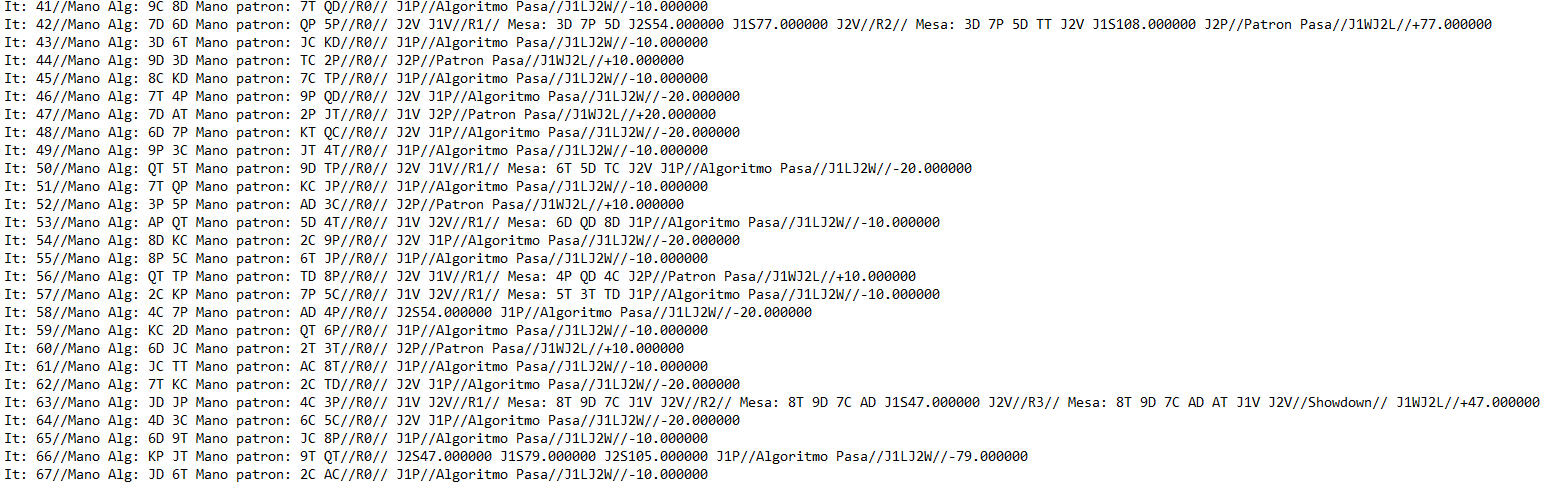
\includegraphics[width=1\textwidth]{figuras/resultados.png}   
\caption{Ejemplo del formato en que se generan los datos}
\label{fig:resultados}
\end{figure}

La idea en que se ha hecho el registro de los datos en el formato explicado en la descripción de los modos del apartado \ref{sec:pokersimu} ha sido para facilitar la transformación y el tratamiento de los datos, ya que al tener un delimitador personalizado (//), permite ser importado por hojas de cálculo de manera bastante eficiente. Un ejemplo de cómo se ven los resultados en bruto se puede ver en \ref{fig:resultados}.

Una vez aplicada una división de columna por delimitador en cada aparición del delimitador, es necesario hacer algunos cambios más\footnote{Cabe destacar que la transformación se ha realizado utilizando Microsoft Excel 2019.Se desconoce si es necesario hacer pasos adicionales o si algunos pasos no son necesarios en caso de que se utilicen otras herramientas para el tratamiento de los datos.}
Debido a que se van añadiendo // con cada ronda, eso implica que se tenga un rellenado de columnas irregular, ya que solamente las rondas en las que se haya alcanzado el River o el Showdown rellenarán por completo todas las columnas, mientras que el resto las rellenarán con un valor \textit{NULL}.  Por lo que es necesario agrupar el resultado de la ronda en una sola columna, para su procesado.

Para esto, se añade una columna condicional en la cual se añadirán cláusulas del tipo \textit{Si(Columna[n]$\neq$NULL)-$>$valor}, tal y como se muestra en la imagen \ref{fig:tf1}. Por el diseño del registro, los valores se almacenan en una diferencia de 2 separaciones, con un máximo de 6 separaciones (entre un resultado del preflop y un resultado del River/Showdown).
\begin{figure}[h]
\centering
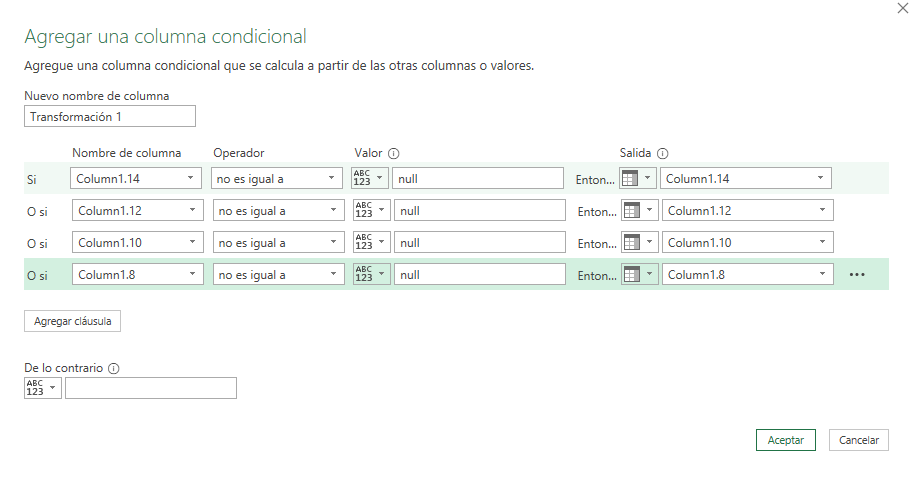
\includegraphics[width=1\textwidth]{figuras/transformacion1.png}   
\caption{Ejemplo de las cláusulas de la columna condicional en la transformación de datos}
\label{fig:tf1}
\end{figure}

Una vez unificados todos los resultados en una misma columna, se ha necesitado hacer 3 transformaciones más:

\begin{enumerate}
\item Conversión de tipo de la columna condicional: debido a que el tipo de importación ha sido desde texto/csv, el tipo de dato estaba definido como texto, por lo que se transforma el tipo de dato en numérico.
\item Reducción de escala: Debido a que los valores de apuesta en el motor de juego eran un tipo de variable float, a la hora de almacenarlos en el registro ha almacenado estos 6 decimales. El problema se ha generado por la diferencia de notación a la hora de escribir los decimales entre Excel y Visual Studio: Visual estudio utiliza "." para comenzar la numeración decimal, mientras que excel utiliza "," y tiene codificado que un "." se utiliza como separación de millares, por lo que al hacer laconversión, se tiene que la columna de resultados está multiplicada por $10^6$, por lo que ha sido necesario crear una nueva columna cuyo valor sea la dicisión del valor de esta columna condicional entre $10^6$. Esta columna es el Beneficio Neto, o resultado Neto, de cada una de las manos de ese registro.
\item Cambio de unidades de Resultado Neto: Tal y como se ha mencionado en el apartado \ref{sec:toma}, la unidad establecida del beneficio es la ciega grande (\textit{ BB}), por lo que para tener el resultado en esta unidad es necesario dividir el resultado Neto por el valor de \textit{BB}. Tal y como se especificó en el apartado \ref{sec:abstracciones}, la ciega grande tiene un valor de 20 para todas las tomas de datos, por lo que se añadirá una última columna como división del valor de Beneficio Neto/20.
\end{enumerate}

Esta última columna, Resultado (BB), será la utilizada de cara a los cálculos y el análisis de los datos.

Una vez realizada la transformación de todos los datos, se procede al estudio de los mismos.

\section{Modo Patrón vs Patrón}
\label{sec:pvp}

En este apartado se van a exponer los resultados de los datos obtenidos. Cabe destacar que, aunque las medidas hayan sido 500 por cada combinación de dos patrones, cada uno de los tres patrones ha participado en 1000 medidas: 500 como jugador[0] y 500 como jugador[1].

Ya que el, por las abstracciones que se tomaron a la hora de plantear el diseño (vease apartado \ref{sec:abstracciones} las partidas son un juego Suma-Cero, si un jugador tiene una ganancia X, el otro jugador tiene una pérdida X. Es decir, el resultado de un jugador es el opuesto del resultado del otro jugador.

Por tanto, para el estudio de cada uno de los patrones, realmente se han utilizado un total de 1000 valores: los valores en los que ese patrón ha sido jugador[0] y el opuesto de los valores en los que ese patrón ha sido jugador[1].

Para este estudio, una vez obtenidos los datos se han calculado la media ($\bar{x}$), varianza($\sigma^2$), desviación típica ($\sigma$) y coeficiente de variación (C.V.)

\subsection{Maniaco}

Este patrón, caracterizado por la agresividad a la hora de jugar y como acción predominante Subir ha obtenido unos resultados bastante positivos frente a los otros patrones.



\begin{figure}[h]
\centering
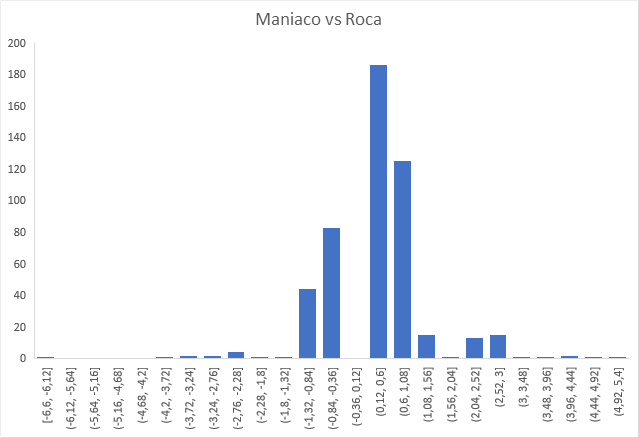
\includegraphics[width=1\textwidth]{figuras/MvR.png}   
\caption{Gráfica Maniaco vs Roca}
\label{fig:MvR}
\end{figure}

\begin{figure}[h]
\centering
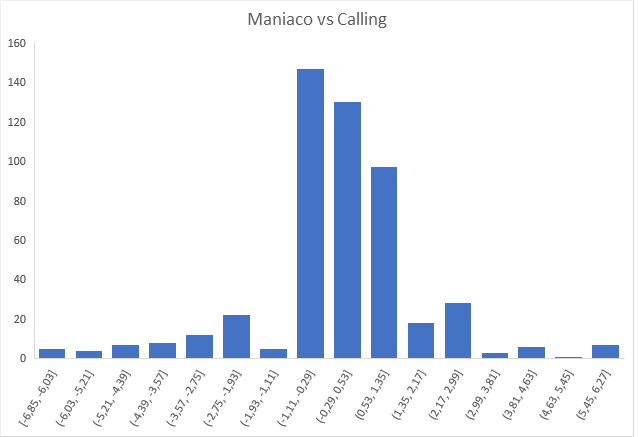
\includegraphics[width=1\textwidth]{figuras/MvC.png}   
\caption{Gráfica Maniaco vs Calling Station}
\label{fig:MvC}
\end{figure}

\begin{figure}[h]
\centering
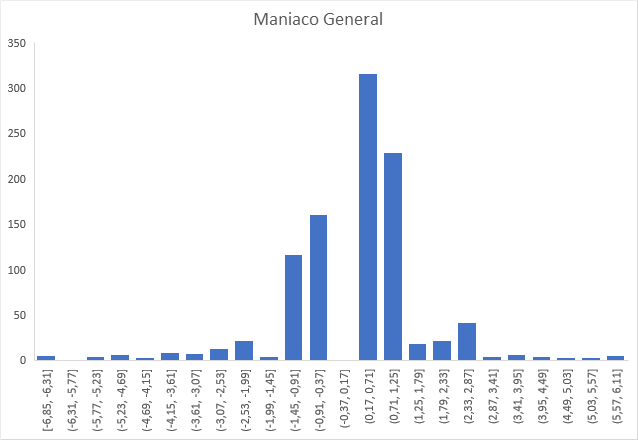
\includegraphics[width=1\textwidth]{figuras/MG.png}   
\caption{Gráfica de Resultados de Maniaco Patrón vs Patrón}
\label{fig:MGR}
\end{figure}

\begin{longtable}[c]{lrrr}
\hline
Maniaco & Vs Roca & Vs Calling & General \\ \hline
$\bar{x}$ & 0,4257 & 0,0434 & 0,23455 \\ 
$\sigma^2 $& 1,19822095 & 3,46452549 & 2,36561441 \\ 
$\sigma$ & 1,09463279 & 1,86132359 & 1,5380554 \\
C.V. & 2,57137137 & 42,8876402 & 6,55747346 \\ \hline
\end{longtable}

El resultado final del patrón Maniaco es $0,23455\pm1,5380554$ $\frac{bb}{partida}$.

Al observar estos datos, se puede deducir que este patrón es el que ha obtenido el mejor resultaado por encima de los otros dos, ya que es el único que tiene una media positiva, tanto contra otros patrones como el resultado general. También es el patrón con la desviación más alta de los tres por lo que los resultados esperados del patrón maniáco tienen mayor rango (pudiendo generar ganancias mayores, pero también pérdidas de mayor cantidad).

\newpage

\subsection{Roca}

Estos son los resultados del patrón Roca, el más pasivo que los demás, teniendo como acción predominante pasar, por lo que acaba jugando muy pocas manos pero las pocas que juega son porque tiene una mano buena.

\begin{figure}[h]
\centering
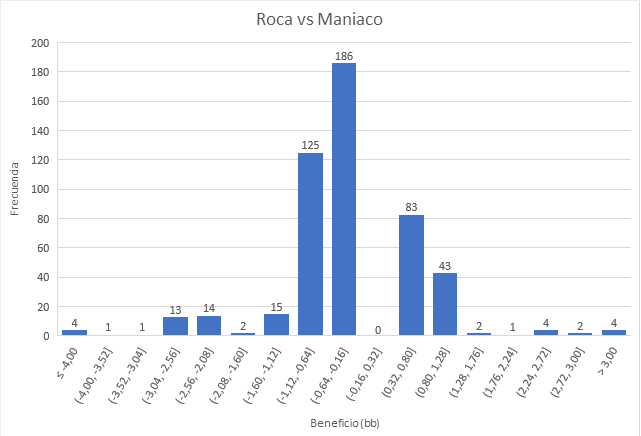
\includegraphics[width=1\textwidth]{figuras/RvM.png}   
\caption{Gráfica Roca vs Maniaco}
\label{fig:RvM}
\end{figure}

\begin{figure}[h]
\centering
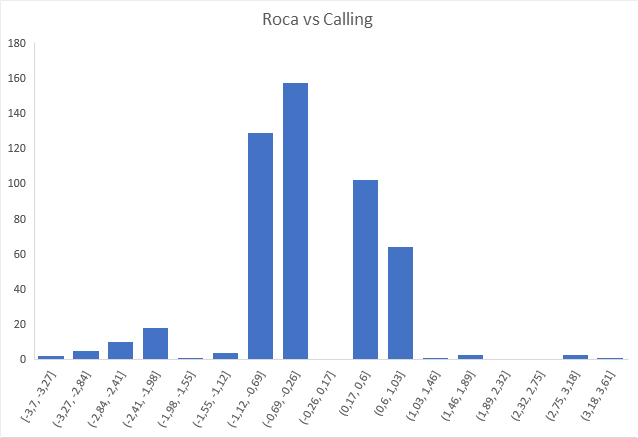
\includegraphics[width=1\textwidth]{figuras/RvC.png}   
\caption{Gráfica Roca vs Calling Station}
\label{fig:RvC}
\end{figure}

\begin{figure}[h]
\centering
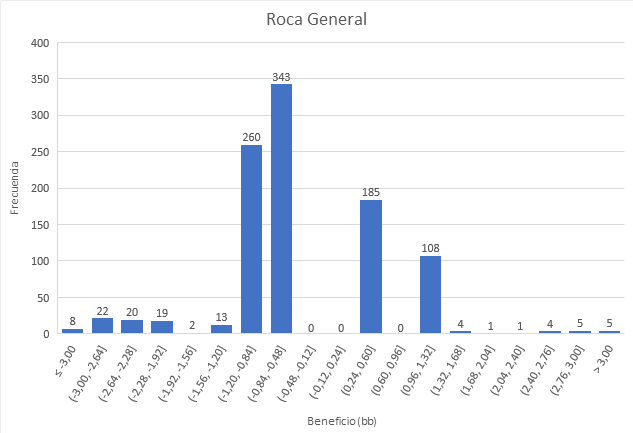
\includegraphics[width=1\textwidth]{figuras/RG.png}   
\caption{Gráfica de Resultados de Roca  Patrón vs Patrón}
\label{fig:RGR}
\end{figure}


\begin{longtable}[c]{lrrr}
\hline
Roca & vs Calling & vs Maniaco & General \\ \hline
$\bar{x}$ & -0,3371 & -0,4257 & -0,3814 \\
$\sigma^2$ & 0,95773406 & 1,19822095 & 1,0788629 \\ 
$\sigma$ & 0,97863888 & 1,09463279 & 1,03868325 \\ 
C.V. & -2,90311148 & -2,57137137 & -2,72334361 \\ \hline
\end{longtable}

El resultado final del patrón Roca es $-0,3814\pm1,03868325$ $\frac{bb}{partida}$.

\smallskip

Observando estos datos, se puede deducir que este patrón es el que ha obtenido el peor valor de media de los 3 (siendo el único que tiene una media general negativa).También es el patrón con la desviación más pequeña de los tres, lo que significa que es el patrón que presenta los datos más compactos.

\clearpage

\subsection{Calling Station}

Aquí se presentan los datos del patrón Calling station, un patrón intermedio entre ambos, pues su acción predominante es ver la apuesta, lo que significa que acaba jugando más apuestas, pero no mete la presión de un maniaco.

\begin{figure}[h]
\centering
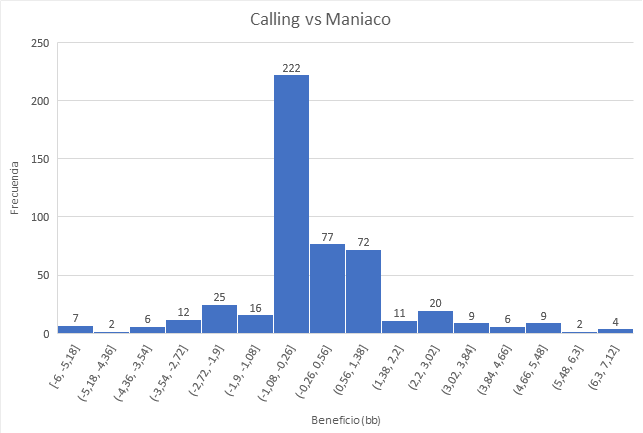
\includegraphics[width=1\textwidth]{figuras/CvM.png}   
\caption{Gráfica Calling Station vs Maniaco}
\label{fig:CvM}
\end{figure}

\begin{figure}[h]
\centering
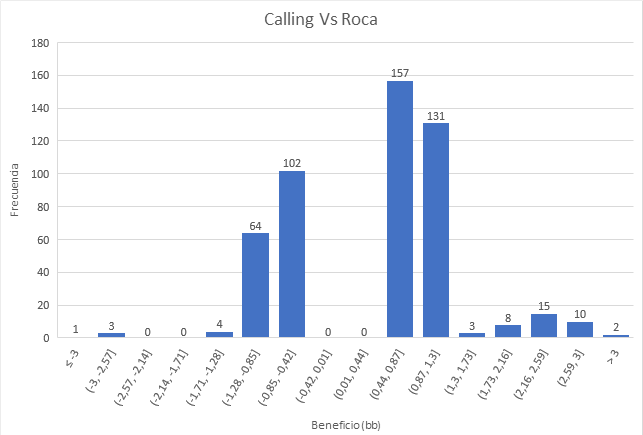
\includegraphics[width=1\textwidth]{figuras/CvR.png}   
\caption{Gráfica Calling Station vs Roca}
\label{fig:CvR}
\end{figure}

\begin{figure}[h]
\centering
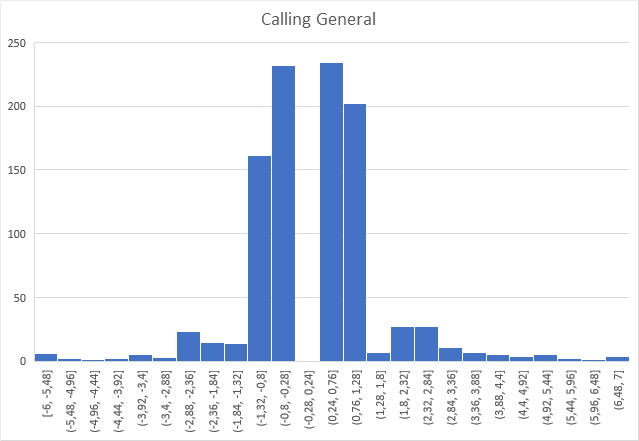
\includegraphics[width=1\textwidth]{figuras/CG.png}   
\caption{Gráfica de Resultados de Calling Station Patrón vs Patrón}
\label{fig:CGR}
\end{figure}

\begin{longtable}[c]{lrrr}
\hline
Calling Station & Vs Maniaco & vs Roca & General \\ \hline
$\bar{x}$ & -0,0434 & 0,3371 & 0,14685 \\ 
$\sigma^2$ & 3,46452549 & 0,95773406 & 2,24514773 \\ 
$\sigma$ & 1,86132359 & 0,97863888 & 1,4983817 \\ 
C.V. & -42,8876402 & 2,90311148 & 10,2034845 \\ \hline
\end{longtable}


El resultado final del patrón Calling Station es $ 0,14685\pm1,4983817$  $\frac{bb}{partida}$.

\smallskip

Observando estos datos, se puede razonar que este patrón tiene unos resultados mixtos, pues si bien tiene una media posivita, su media es menor que la de Maniaco, y su desviación media es menor que la de Maniaco también, pero bastante cercana, lo cual no convierte sus datos en un conjunto tan compacto como lo sería un jugador más defensivo.

\clearpage

\subsection{Discusión sobre los datos obtenidos en el modo Patrón vs Patrón}

Se agrupan los resultados finales en este apartado, para poder hacer una comparación más sencilla entre los 3

\vspace{5mm} %5mm vertical space

Maniaco:  $0,23455\pm1,5380554$ $\frac{bb}{partida}$.

Roca: $-0,3814\pm1,03868325$ $\frac{bb}{partida}$.

Calling Station: $ 0,14685\pm1,4983817 $ $\frac{bb}{partida}$.

\vspace{5mm} %5mm vertical space
Estos datos son los esperados en esta comparació entre patrones, pues si únicamente se mantiene una de las 3 acciones posibles como predominante, Maniaco genera más victorias y más rentabilidad, pues la presión que ejerce con las constantes subidas hace que muchos oponentes pasen una mano por miedo a que tenga una buena mano. Las subidas constantes provocan también un aumento de la varianza y, por tanto, de la desviación, pues hay mayor dinero apostado, lo que significa que las variaciones de dinero también serán mayores.

En el extremo opuesto del espectro se encontraría el jugador defensivo, en este caso, Roca. Pues sus estrategias hacen que, si bien el número de apuestas perdidas aumente, las pocas que  juege seguramente las gane. Al participar tan poco en las apuesas, provoca una desviación mucho menor, ya que, al intentar minimizar pérdidas jugando defensivo, tampoco se pueden llegar a generar ganancias. 

Y el resultado intermedio lo tiene con Calling Station, donde tiene tanto lo peor de ambos como lo mejor de ambos: si bien juega muchas apuestas, hay menos jugadas que gane a base de intimidar, lo que provoca que su media sea menor que la de Maniaco. También cabe mencionar que, ya que prácticamente siempre ve la  apuesta, su mero comportamiento hace que las apuestas no suban tanto, aunque si que permite que suban.

De estos datos se puede deducir que mantener una única estrategia defensiva no acaba siendo tan beneficioso que una agresiva. También se puede obtener de estos datos que todos tienen cosas favorables y perjudiciales, por lo que sería lógico pensar que mantener siempre una mísma estrategia acaba siendo perjudicial, pues, a la larga, los jugadores acaban adaptándose al ritmo de subidas, forzando algunas pérdidas. Pero en pocos juegos, acaba siendo más ventajosa maniaco.

\section{Modo Algoritmo vs Patrón}


En este apartado se procede a analizar los datos obtenidos por el Modo Algoritmo vs Patrón, primero analizándolos inidividualmente con cada patrón y, posteriormente, con el cómputo total de los datos de este modo, para obtener el resultado del experimento.

A diferencia del modo Patrón vs Patrón, aquí se analizarán tanto los Cuartiles $Q_1$, $Q_2$, $Q_3$, que corresponden a los percentiles $P_{25}$, $P_{50}$, $P_{75}$, así como el estudio de las victorias.

\subsection{Discusión previa y explicación de las medidas}
\label{sec:predisc}

En este caso, los datos de los que dispone y su exposición puede que no sean de todo intuitivos. Inicialmente se tomaron 2 medidas de datos del algoritmo enfrentándose a cada uno de loa patrones (que son G1 y G2), pero al hacer un análisis previo de estos datos, se llegó a la conclusión de que había algo que no rondaba bien. Esto que se detecto fue que, en unas cuantas rondas en las que, aun teniendo todos los datos a favor, el algoritmo pasaba la apuesta.

Siguiendo los datos de depurador y del servidor API, los cálculos eran correctos, pero esa decisión no era problema del algoritmo, sino de que el valor que aleatorizaba la salida habia sacado un valor prácticamente 0, por lo que se generó el "Pasar"

Si bien esa era una de las premisas iniciales del proyecto (que el algoritmo fuera, en parte, imprevisible), en este punto esta premisa puede no ser tan acertada. Por lo que se decidió probar a tomar medidas eliminando dicho factor aleatorio y dejando únicamente la opción con más peso (manteniendo la probabilidad de hacer faroles de la misma manera que estaba diseñada). 
Con esta modificación se generó una tanda de datos para cada patrón (GE).

Para poder hacer una comparación adecuada y un total del enfrentamiento contra cada patrón, lo planteado era repetir las dos tandas de datos, pero por imposibilidades físicas se pudo realizar la segunda toma con el motor de juego modificado. 

Por lo que los datos de los que se dispone es G1, G2 y G3. 

Puesto que se va a aprovechar y utilizar estos datos para hacer una comparativa del total del funcionamiento, es necesario ponderar para la agrupación de datos (T). De no hacerlo, los resultados con el factor aleatorio tendrían un peso del 66.67\% sobre el total.

Por este motivo, se aplicará un modificador de 0.5 a los datos G1 y G2 \textbf{solamente para los cálculos de T} . Para las comparativas de histogramas, Cuartiles, y los valores descriptivos estadísticos individuales, se tomará el valor original.

\subsection{Estudio del enfrentamiento individual de Algoritmo vs Patrón}
\label{sec:AvP}

En este apartado, se expondrán los datos de los enfrentamientos de manera individual, sin tener en consideración los datos de losenfrentamientos con otros patrones. 

\subsubsection{Algoritmo vs Maniaco}

Se procede a desarrollar el resultado de las dos iteracciones con Maniaco, empezando por los resultados de beneficio

\begin{longtable}[c]{lrrrr}
\hline
Algoritmo vs Maniaco & G1 & G2 & GE & T \\ \hline
$\bar{x}$ & -0,4847 & -0,3566 & -0,2881 & -0,37646667 \\ 
$\sigma$ & 1,468904663 & 1,83463251 & 2,49953263 & 1,98251848 \\ 
$\sigma^2$  & 2,15768091 & 3,36587644 & 6,24766339 & 3,93037952 \\ 
C.V. & -3,030543972 & -5,14479111 & -8,67592029 & -5,26611956 \\ 
$Q_1$ & -1,108333333 & -1,04719198 & -1,214375 & -0,73288462 \\
$Q_2$ & -0,648275862 & -0,75707736 & -0,46176471 & -0,30397351 \\ 
$Q_3$ & -0,248029557 & -0,46696275 & 9,77254902 & 0,07475166 \\ \hline
\caption{Tabla Algoritmo vs Maniaco}
\label{tab:AvM}
\end{longtable}


\begin{figure}[h]
\centering
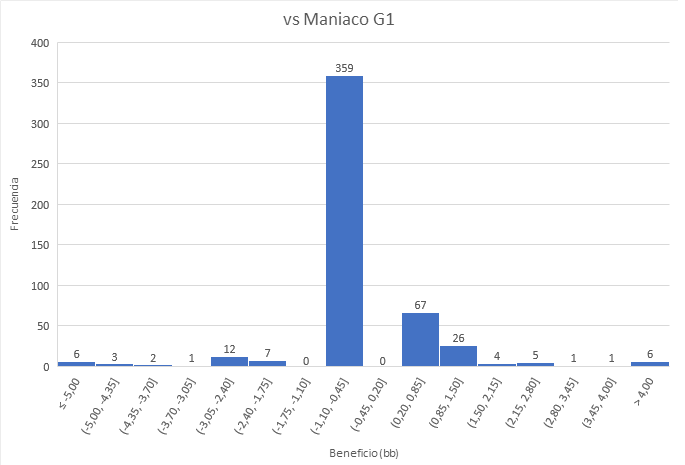
\includegraphics[width=1\textwidth]{figuras/AvMG1.png}   
\caption{Gráfica Algoritmo vs Maniaco (G1)}
\label{fig:AvMG1}
\end{figure}

\begin{figure}[h]
\centering
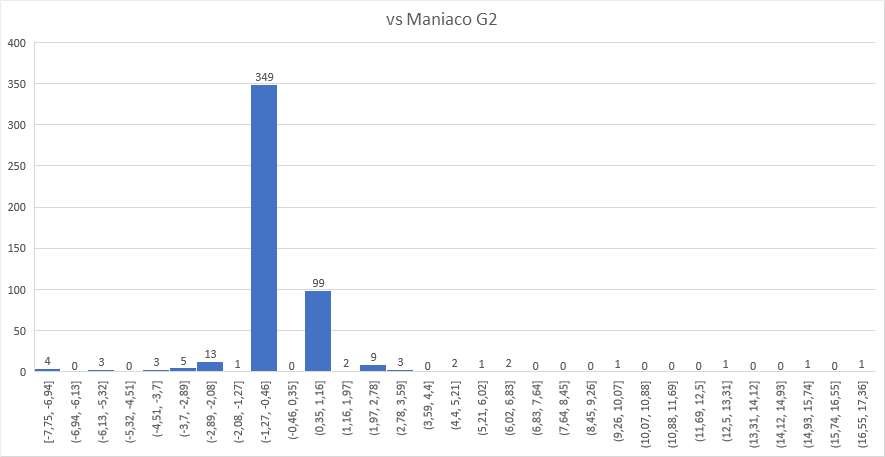
\includegraphics[width=1\textwidth]{figuras/AvMG2.png}   
\caption{Gráfica Algoritmo vs Maniaco (G2)}
\label{fig:AvMG2}
\end{figure}


\begin{figure}[h]
\centering
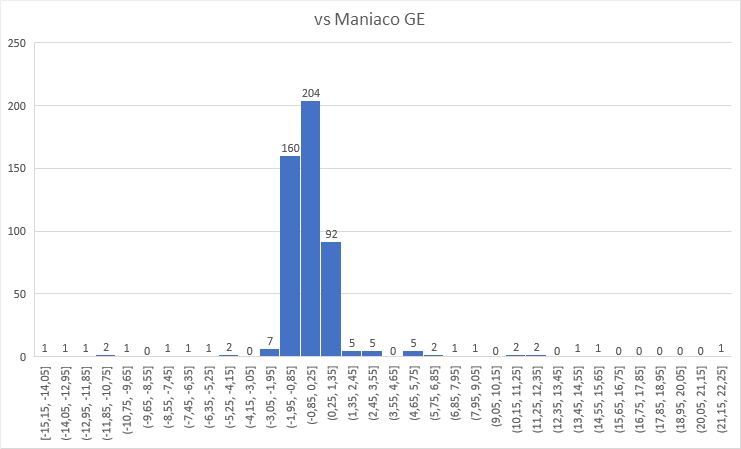
\includegraphics[width=1\textwidth]{figuras/AvMGE.png}   
\caption{Gráfica Algoritmo vs Maniaco (GE)}
\label{fig:AvMGE}
\end{figure}

\begin{figure}[h]
\centering
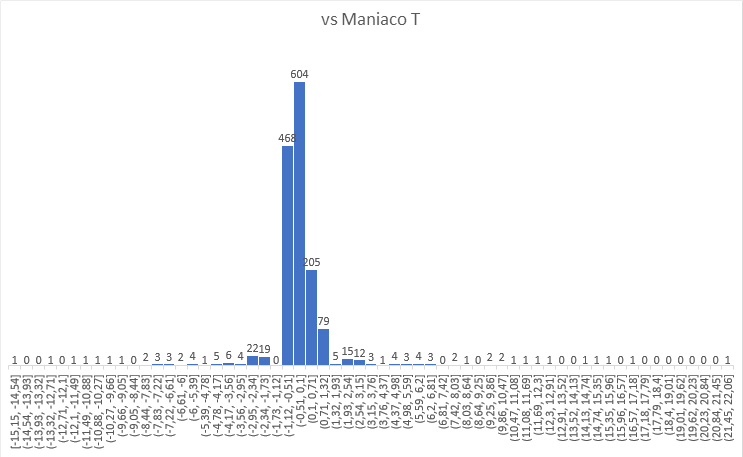
\includegraphics[width=1\textwidth]{figuras/AvMT.png}   
\caption{Gráfica Algoritmo vs Maniaco (T)}
\label{fig:AvMGT}
\end{figure}

\vspace{5mm} %5mm vertical space

Ahora se procede a estudiar el desarrollo de las partidas en cada uno de los conjuntos de los datos, estudiando primero el número de victorias generales, el número de partidas que han acabado en una determinada ronda (y el desglose de victorias/derrotas de esas partidas), así como calcular el porcentaje de victorias respecto a las rondas que acaban en esa ronda.

\vspace{5mm} %5mm vertical space

\begin{longtable}[c]{lrrrr}
\hline
Algoritmo vs Maniaco & G1 & G2 & GE & T \\ \hline
Nº Partidas & 500 & 500 & 500 & 1500 \\ 
Nº Victorias & 110 & 122 & 118 & 350 \\ 
Nº Derrotas & 390 & 378 & 382 & 1150 \\ 
Partidas Fin Preflop & 406 & 410 & 404 & 1220 \\ \
Nº Victorias preflop & 80 & 92 & 71 & 243 \\ 
Nº Derrotas Preflop & 326 & 318 & 333 & 977 \\ 
Partidas Fin Flop & 60 & 57 & 56 & 173 \\ 
Nº Victorias Flop & 15 & 14 & 28 & 57 \\ 
Nº Derrotas Flop & 45 & 43 & 28 & 116 \\ 
Partidas Fin Turn & 23 & 23 & 23 & 69 \\ 
Nº Victorias Turn & 8 & 11 & 10 & 29 \\ 
Nº Derrotas Turn & 15 & 12 & 13 & 40 \\ 
Partidas Fin River & 8 & 4 & 3 & 15 \\ 
Nº VictoriasRiver & 6 & 1 & 0 & 7 \\ 
Nº Derrotas River & 2 & 3 & 3 & 8 \\ 
Partidas Fin Showdown & 3 & 6 & 14 & 23 \\ 
Nº Victorias Swodown & 1 & 4 & 9 & 14 \\ 
Nº Derrotas Showdown & 2 & 2 & 5 & 9 \\ \hline
\caption{Desglose de las partidas contra Maniaco}
\label{tab:PlaysM}
\end{longtable}

\begin{longtable}[c]{lrrrr}
\hline
\% Victoria vs Maniaco & G1 & G2 & GE & T \\ \hline
General & 22,000\% & 24,400\% & 23,600\% & 23,333\% \\ 
Preflop & 19,704\% & 22,439\% & 17,574\% & 19,918\% \\ 
Flop & 25,000\% & 24,561\% & 50,000\% & 32,948\% \\ 
Turn & 34,783\% & 47,826\% & 43,478\% & 42,029\% \\ 
River & 75,000\% & 25,000\% & 0,000\% & 46,667\% \\ 
Showdown & 33,333\% & 66,667\% & 64,286\% & 60,870\% \\ \hline
\caption{Porcentajes de victoria Algoritmo vs Maniaco (Desglose por rondas)}
\label{tab:winrateM}
\end{longtable}

El resultado final del enfrentamiento contra el patrón Maniaco es $-0.3764667\pm1.982518$ $\frac{bb}{partida}$.

\vspace{5mm} %5mm vertical space

Teniendo todos los datos de los enfrentamientos contra Maniaco, se puede encontrar que GE supone una mejora de la media con respecto tanto a G1 y G2. Si buen aumentá la desviación típica, cabe destacar de estos datos el valor de $Q_3$, en el que se puede apreciar un incremento de mas de 10 puntos, lo que significa que el beneficio que se ha obtenido ha sido considerablemente mayor al de G1 y G2. Esto, en el caso de $Q_1$ no ocurre, pues, si bien es cierto que el valor es menor, el descenso no es tan significativo como el incremento de $Q_3$. 
Lo último reseñable de estos datos es el análisis de las victorias. 
Si bien es cierto que las victorias totales no se han incrementado, en concreto son peores que G2, lo que si se ha visto un incremento significativo es el número de las partidas que llegan hasta el showdown, ganando 9 de las 14 partidas. 

\clearpage

\subsubsection{Algoritmo vs Roca}

Se procede a desarrollar el resultado de las dos iteracciones con Roca, empezando por los resultados de beneficio

\begin{longtable}[c]{lrrrr}
\hline
Algoritmo vs Roca & G1 & G2 & GE & T \\ \hline
$\bar{x}$ & -0,188 & -0,1133 & -0,2538 & -0,13481667 \\ 
$\sigma$ & 0,8878415 & 0,90963343 & 0,7136555 & 0,55795976 \\
$\sigma^2$& 0,78826253 & 0,82743298 & 0,50930417 & 0,3113191 \\
C.V. & -4,72256116 & -8,02853865 & -2,81188139 & -4,13865567 \\ 
$Q_1$ & -0,98572581 & -0,62575758 & -0,71976378 & -0,5248427 \\ 
$Q_2$ & -0,34 & -0,37323232 & -0,53306604 & -0,20319338 \\ 
$Q_3$ & 0,37567568 & 0,37068966 & 0,31245614 & 0,345837 \\ \hline
\caption{Tabla Algoritmo vs Roca}
\label{tab:AvR}
\end{longtable}



\begin{figure}[h]
\centering
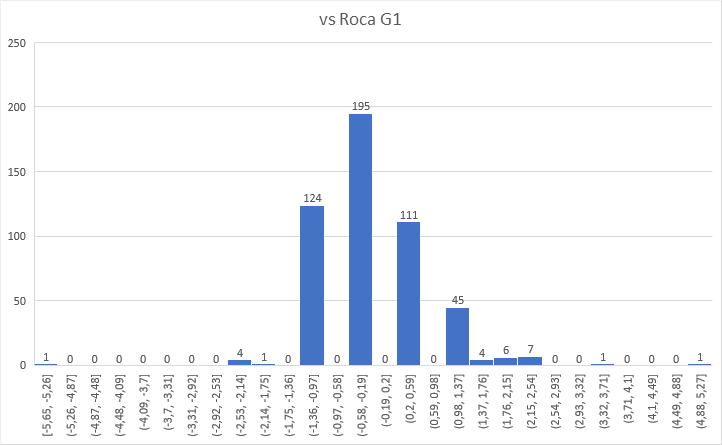
\includegraphics[width=1\textwidth]{figuras/AvRG1.png}   
\caption{Gráfica Algoritmo vs Roca(G1)}
\label{fig:AvRG1}
\end{figure}

\begin{figure}[h]
\centering
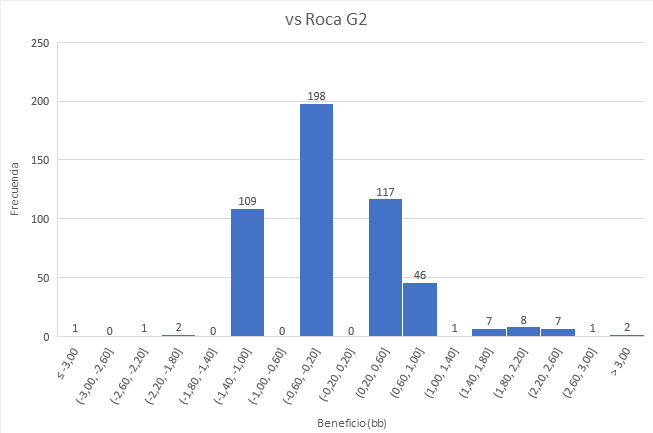
\includegraphics[width=1\textwidth]{figuras/AvRG2.png}   
\caption{Gráfica Algoritmo vs Roca (G2)}
\label{fig:AvRG2}
\end{figure}


\begin{figure}[h]
\centering
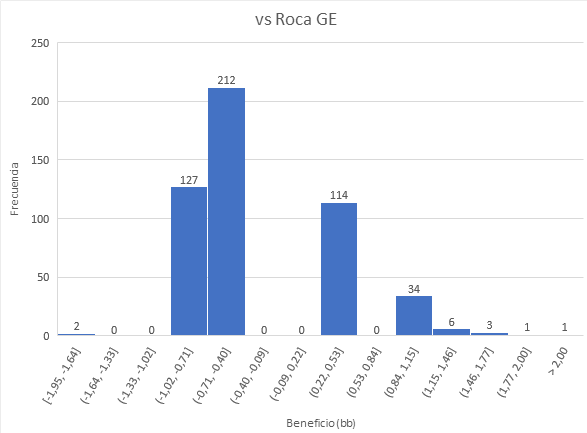
\includegraphics[width=1\textwidth]{figuras/AvRGE.png}   
\caption{Gráfica Algoritmo vs Roca (GE)}
\label{fig:AvRGE}
\end{figure}

\begin{figure}[h]
\centering
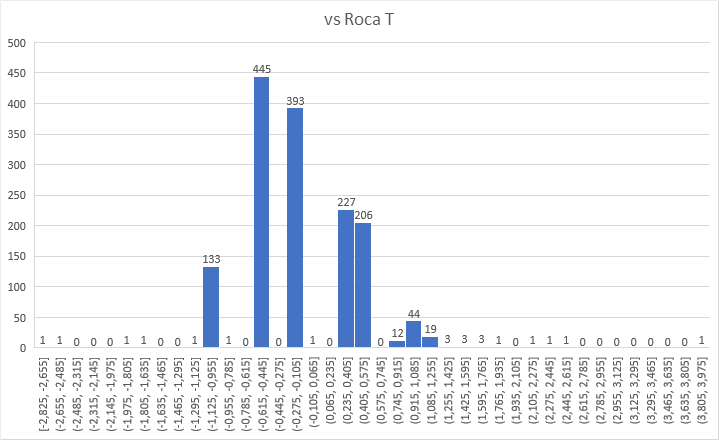
\includegraphics[width=1\textwidth]{figuras/AvRT.png}   
\caption{Gráfica Algoritmo vs Roca (T)}
\label{fig:AvRGT}
\end{figure}

Ahora se procede a estudiar el desarrollo de las partidas en cada uno de los conjuntos de los datos, estudiando primero el número de victorias generales, el número de partidas que han acabado en una determinada ronda (y el desglose de victorias/derrotas de esas partidas), así como calcular el porcentaje de victorias respecto a las rondas que acaban en esa ronda.


\begin{longtable}[c]{lrrrr}
\hline
Algoritmo vs Roca & G1 & G2 & GE & T \\ \hline
Nº Partidas & 500 & 500 & 500 & 1500 \\ 
Nº Victorias & 175 & 189 & 159 & 523 \\ 
Nº Derrotas & 325 & 311 & 341 & 977 \\ 
Partidas Fin Preflop & 378 & 389 & 400 & 1167 \\ 
Nº Victorias preflop & 79 & 99 & 86 & 264 \\ 
Nº Derrotas Preflop & 299 & 290 & 314 & 903 \\ 
Partidas Fin Flop & 115 & 104 & 94 & 313 \\ 
Nº Victorias Flop & 92 & 85 & 70 & 247 \\ 
Nº Derrotas Flop & 23 & 19 & 24 & 66 \\ 
Partidas Fin Turn & 5 & 6 & 5 & 16 \\ 
Nº Victorias Turn & 3 & 4 & 2 & 9 \\ 
Nº Derrotas Turn & 2 & 2 & 3 & 7 \\ 
Partidas Fin River & 1 & 1 & 0 & 2 \\ 
Nº VictoriasRiver & 1 & 1 & 0 & 2 \\ 
Nº Derrotas River & 0 & 0 & 0 & 0 \\ 
Partidas Fin Showdown & 1 & 0 & 1 & 2 \\ 
Nº Victorias Swodown & 0 & 0 & 1 & 1 \\ 
Nº Derrotas Showdown & 1 & 0 & 0 & 1 \\ \hline
\caption{Desglose de las partidas contra Roca}
\label{tab:PlaysR}
\end{longtable}

\begin{longtable}[c]{lrrrr}
\hline
\% Victoria vs Roca & G1 & G2 & GE & T \\ \hline
General & 35,000\% & 37,800\% & 31,800\% & 34,867\% \\ 
Preflop & 20,899\% & 25,450\% & 21,500\% & 22,622\% \\ 
Flop & 80,000\% & 81,731\% & 74,468\% & 78,914\% \\ 
Turn & 60,000\% & 66,667\% & 40,000\% & 56,250\% \\ 
River & 100,000\% & 100,000\% & - & 100,000\% \\ 
Showdown & 0,000\% & - & 100,000\% & 50,000\% \\  \hline
\caption{Porcentajes de victoria Algoritmo vs Roca (Desglose por rondas)}
\label{tab:winrateR}
\end{longtable}

El resultado final del enfrentamiento contra el patrón Roca es $-0.13481667\pm0.55795976$ $\frac{bb}{partida}$.

\vspace{5mm} %5mm vertical space

Cabe destacar que en la segunda toma de datos, no se llegó al Showdown en ninguna partida, mientras que en GE la única que se llegó a River, se continuó hasta el Showdown, por lo que ningua termino en River tampoco.

Si bien en el caso del Maniaco se encontraba con una reseñable mejora de GE con respecto de G1 y G2, no ocurre lo mismo en el caso contra Roca. En este caso se tiene, tanto una bajada de la media como de $Q_2$. Si bien es cierto estos datos por separado no tienen por qué ser un mal indicio, nos encontramos un descenso de la desviación (centralizando más los datos en torno a la media) y un descenso de las victorias de la ronda (al igual que no se encuentra ninguna mejoría de rondas que se llega hasta el Showdown). 


\clearpage


\subsubsection{Algoritmo vs Calling Station}

Se procede a desarrollar el resultado de las dos iteracciones contra Calling Station, empezando por los resultados de beneficio

\begin{longtable}[c]{lrrrr}
\hline
Algoritmo vs Calling Station & G1 & G2 & GE & T \\ \hline
$\bar{x}$ & -0,33416834 & -0,315 & -0,3085 & -0,21091667 \\ 
$\sigma$ & 1,12701073 & 1,07291426 & 0,84380255 & 0,67335509 \\ 
$\sigma^2$ & 1,2701532 & 1,151145 & 0,71200275 & 0,45340708 \\ 
C.V. & -3,37258385 & -3,406077 & -2,73517846 & -3,19251724 \\ 
Q1 & -1,08380282 & -0,87428571 & -0,9629932 & -0,57929293 \\ 
Q2 & -0,72918782 & -0,5308377 & -0,35323944 & -0,42164948 \\ 
Q3 & 0,13241758 & 0,29922222 & 0,25288889 & 0,19530387 \\ \hline
\caption{Tabla Algoritmo vs Calling Station}
\label{tab:AvC}
\end{longtable}


\begin{figure}[h]
\centering
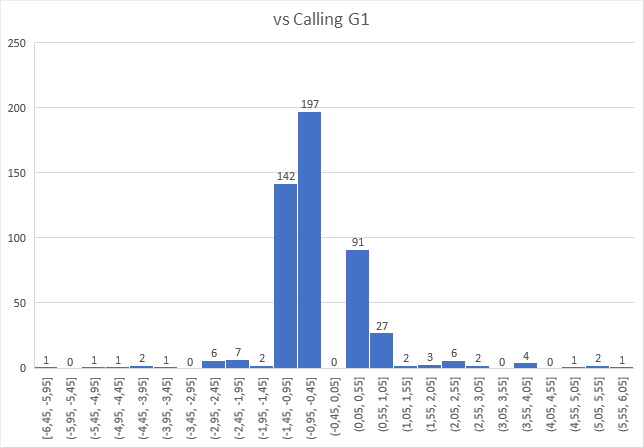
\includegraphics[width=1\textwidth]{figuras/AvCG1.png}   
\caption{Gráfica Algoritmo vs Calling Station (G1)}
\label{fig:AvRC1}
\end{figure}

\begin{figure}[h]
\centering
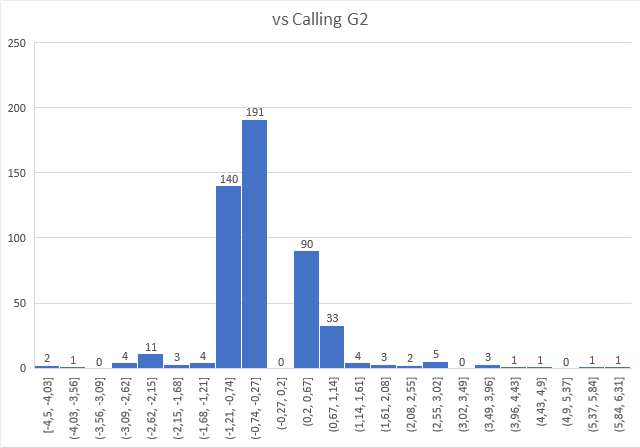
\includegraphics[width=1\textwidth]{figuras/AvCG2.png}   
\caption{Gráfica Algoritmo vs Calling Station (G2)}
\label{fig:AvRC2}
\end{figure}


\begin{figure}[h]
\centering
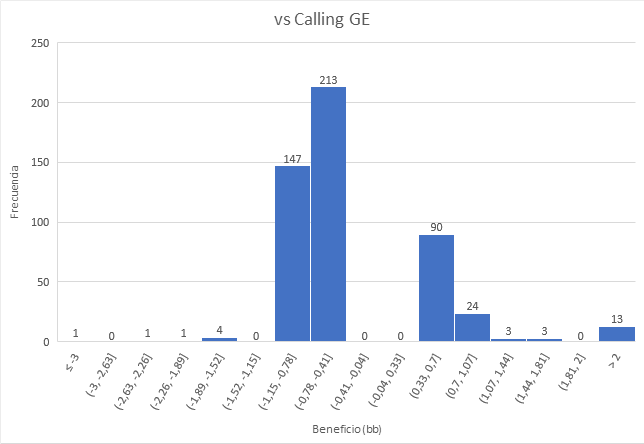
\includegraphics[width=1\textwidth]{figuras/AvCGE.png}   
\caption{Gráfica Algoritmo vs Calling Station (GE)}
\label{fig:AvRCE}
\end{figure}

\begin{figure}[h]
\centering
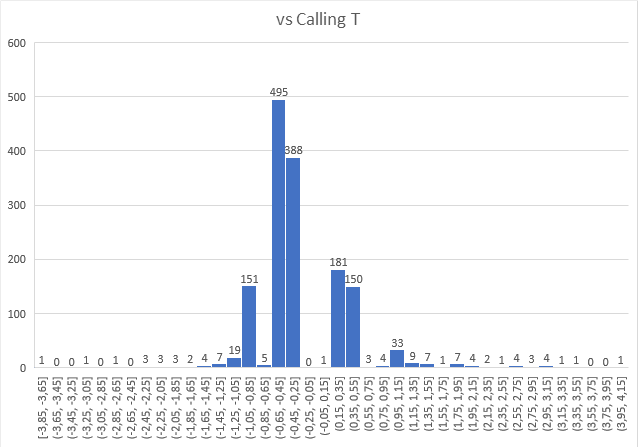
\includegraphics[width=1\textwidth]{figuras/AvCT.png}   
\caption{Gráfica Algoritmo vs Calling Station (T)}
\label{fig:AvRCT}
\end{figure}

Ahora se procede a estudiar el desarrollo de las partidas en cada uno de los conjuntos de los datos, estudiando primero el número de victorias generales, el número de partidas que han acabado en una determinada ronda (y el desglose de victorias/derrotas de esas partidas), así como calcular el porcentaje de victorias respecto a las rondas que acaban en esa ronda.


\begin{longtable}[c]{lrrrr}
\hline
Algoritmo vs Calling Station & G1 & G2 & GE & T \\ \hline
Nº Partidas & 500 & 500 & 500 & 1500 \\ 
Nº Victorias & 139 & 144 & 133 & 416 \\ 
Nº Derrotas & 360 & 356 & 367 & 1083 \\ 
Partidas Fin Preflop & 398 & 382 & 405 & 1185 \\ 
Nº Victorias preflop & 92 & 82 & 83 & 257 \\ 
Nº Derrotas Preflop & 306 & 300 & 322 & 928 \\ 
Partidas Fin Flop & 56 & 82 & 62 & 200 \\ 
Nº Victorias Flop & 26 & 45 & 30 & 101 \\ 
Nº Derrotas Flop & 30 & 37 & 32 & 99 \\ 
Partidas Fin Turn & 26 & 20 & 19 & 65 \\ 
Nº Victorias Turn & 12 & 10 & 8 & 30 \\ 
Nº Derrotas Turn & 14 & 10 & 11 & 35 \\ 
Partidas Fin River & 12 & 12 & 5 & 29 \\ 
Nº VictoriasRiver & 4 & 4 & 5 & 13 \\ 
Nº Derrotas River & 8 & 8 & 0 & 16 \\ 
Partidas Fin Showdown & 8 & 4 & 9 & 21 \\ 
Nº Victorias Swodown & 5 & 3 & 7 & 15 \\ 
Nº Derrotas Showdown & 2 & 1 & 2 & 5 \\ \hline
\caption{Desglose de las partidas contra Calling Station}
\label{tab:PlaysC}
\end{longtable}

\begin{longtable}[c]{lrrrr}
\hline
\% Victoria vs Calling Station & G1 & G2 & GE & Total \\ \hline
General & 27,800\% & 28,800\% & 26,600\% & 27,733\% \\ 
Preflop & 23,116\% & 21,466\% & 20,494\% & 21,688\% \\ 
Flop & 46,429\% & 54,878\% & 48,387\% & 50,500\% \\ 
Turn & 46,154\% & 50,000\% & 42,105\% & 46,154\% \\ 
River & 33,333\% & 33,333\% & 100,000\% & 44,828\% \\ 
Showdown & 62,500\% & 75,000\% & 77,778\% & 71,429\% \\ \hline
\caption{Porcentajes de victoria Algoritmo vs Calling Station (Desglose por rondas)}
\label{tab:winrateC}
\end{longtable}


El resultado final del enfrentamiento contra el patrón Calling Station es $-0.21091667\pm0.67335509$ $\frac{bb}{partida}$.

\vspace{5mm} %5mm vertical space

Aquí cabe destacar los valores de Showdown de G1, en el que hay 8 partidas que han llegado a Showdown, pero hay 5 victorias y 2 derrotas. Estos datos con correctos, pues la partida faltante resultó en empate, por lo que no hay ningún error en el procesado de datos.

Tras esta curiosidad sobre el empate, se procede a estudiar el conjunto de los datos de Calling Station. Siguiendo el hilo de resultados que se encontró en el apartado \ref{sec:pvp}, los resultados de los enfrentamientos con Calling Station son mixtos, aunque con tendencia positiva. Se aumenta ligeramente la media, se disminuye ligeramente la desviación y se puede apreciar una mejoría considerable de la mediana ($Q_2$), si bien los otros dos percentiles no se obtiene una mejora, pero tampoco se tiene un empeoramiento.
Por último, se observa que GE tiene un ligero menor número de victorias.

\clearpage

\subsection{Análisis del los datos por conjuntos}

En este apartado, se procede a estudiar los datos en conjunto, tomando como punto de estudio el origen de los datos. Es decir, se estudiarán los datos obtenidos del enfrentamiento contra los 3 algoritmos simultáneamente, tomando como un conjunto G1 y G2 ,como otro conjunto GE y por últimom T.

\subsubsection{Datos Previos a la modificación (G1 y G2)}

\begin{longtable}[c]{lr}
\hline
G1 y G2 & Valores \\ \hline
$\bar{x}$& -0,29861621 \\ 
$\sigma$ & 1,26776522 \\ 
$\sigma^2$& 1,60722864 \\ 
C.V.& -4,2454669 \\ 
$Q_1$ & -1,03119077 \\ 
$Q_2$ & -0,50274344 \\ 
$Q_3$ & 0,35380952 \\ \hline
\caption{Tabla Resultados comunes G1 y G2}
\label{tab:AGP}
\end{longtable}

\vspace{5mm} %5mm vertical space

El resultado final de los datos de G1 y G2 es $-0,29861621\pm1,26776522$ $\frac{bb}{partida}$.

\vspace{5mm} %5mm vertical space

\begin{figure}[h]
\centering
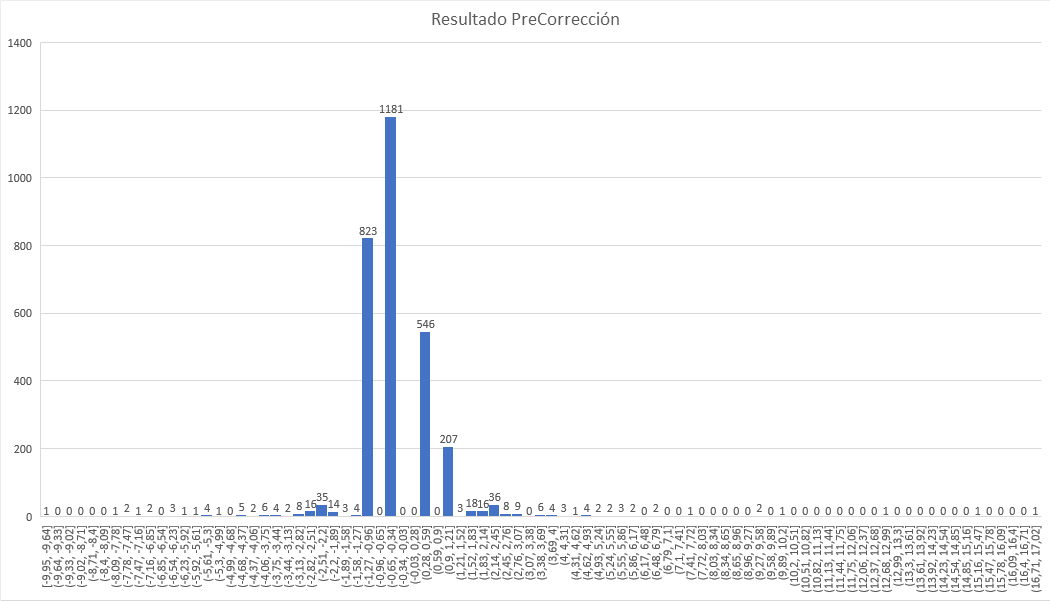
\includegraphics[width=1\textwidth]{figuras/AGP.png}   
\caption{Gráfica resultados Algoritmo G1 y G2}
\label{fig:AGP}
\end{figure}

\newpage

\subsubsection{Datos posteriores a la modificación (GE)}

\begin{longtable}[c]{lr}
\hline
GE & Valores \\ \hline
$\bar{x}$ & -0,28346667 \\ 
$\sigma$ & 1,57791845 \\ 
$\sigma^2$ & 2,48982665 \\ 
C.V. & -5,56650443 \\ 
$Q_1$ & -0,84511521 \\ 
$Q_2$ & -0,52945946 \\ 
$Q_3$ & 0,49235294 \\ \hline
\caption{Tabla Resultados GE}
\label{tab:AGC}
\end{longtable}

\vspace{5mm} %5mm vertical space

El resultado final de los datos de GE es $ -0,28346667\pm1,57791845$$\frac{bb}{partida}$.

\vspace{5mm} %5mm vertical space

\begin{figure}[h]
\centering
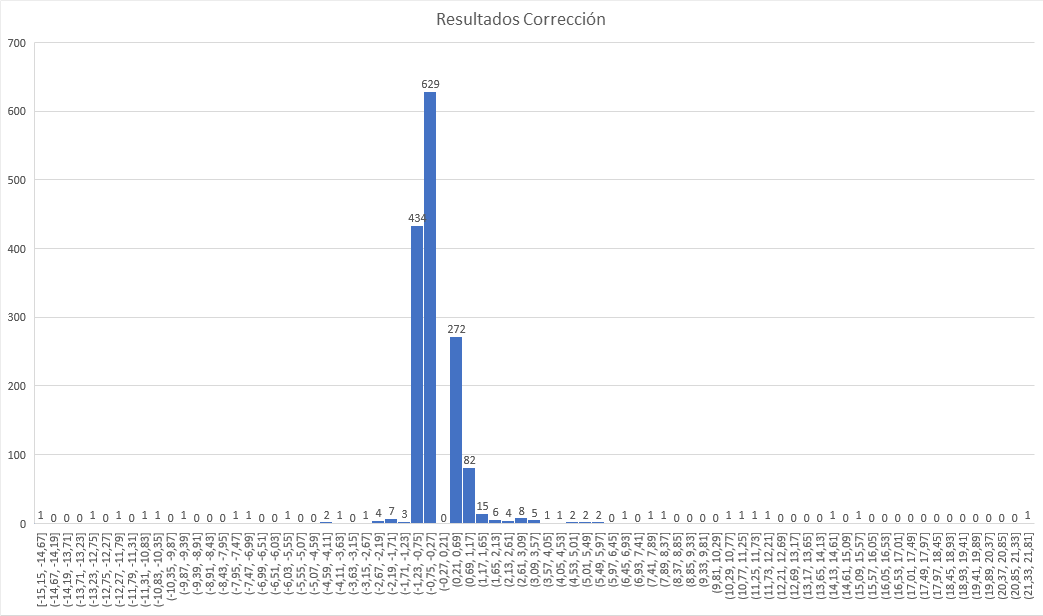
\includegraphics[width=1\textwidth]{figuras/AGC.png}   
\caption{Gráfica resultados Algoritmo GE}
\label{fig:AGC}
\end{figure}


\subsubsection{Datos totales (T)}

\begin{longtable}[c]{lr}
\hline
T & Valores \\ \hline
$\bar{x}$ & -0,19957213 \\ 
$\sigma$ & 1,06969216 \\ 
$\sigma^2$ & 1,14424131 \\ 
C.V. & -5,35992761 \\ 
$Q_1$ & -0,58161924 \\ 
$Q_2$ & -0,39856115 \\ 
$Q_3$ & 0,10397661 \\ \hline
\caption{Tabla Resultados T}
\label{tab:AGT}
\end{longtable}

El resultado final de los datos de T es  $-0,19957213\pm1,06969216$$\frac{bb}{partida}$.


\begin{figure}[h]
\centering
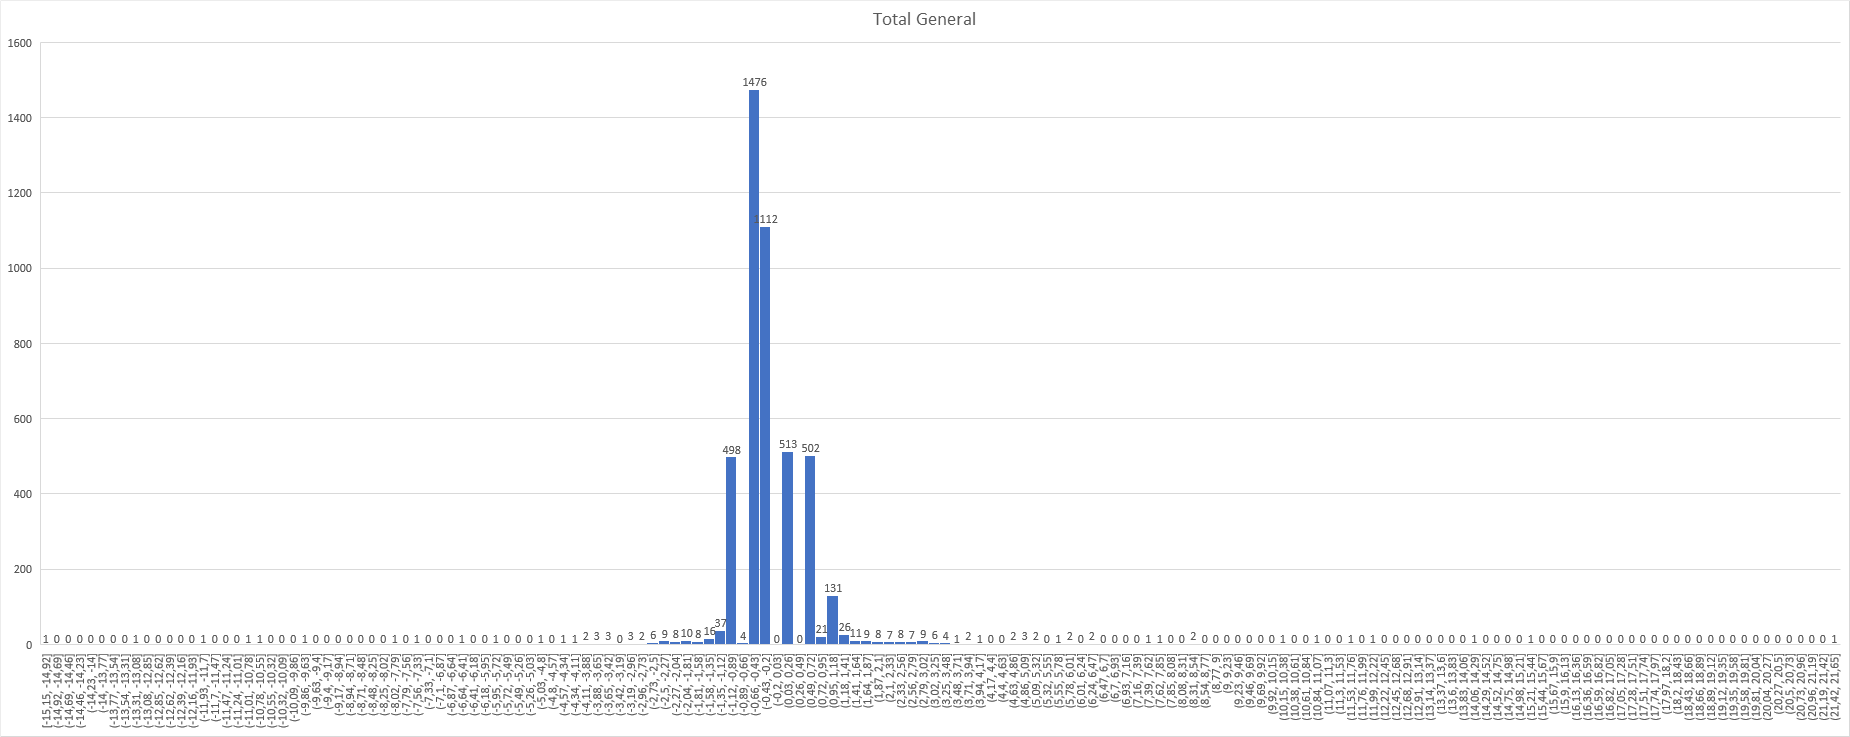
\includegraphics[width=1\textwidth]{figuras/AGT.png}   
\caption{Gráfica resultados Algoritmo T}
\label{fig:AGT}
\end{figure}

\newpage

\subsection{Tasa de victorias de los conjuntos}

\begin{longtable}[c]{lrrr}
\hline
Número de Partidas &  &  &  \\ \hline
Ronda & PreCorrección & Corrección & Total \\ \hline
Partida & 3000 & 1500 & 4500 \\ 
Preflop & 2363 & 1209 & 3572 \\ 
Flop & 474 & 212 & 686 \\ 
Turn & 103 & 44 & 147 \\ 
River & 38 & 8 & 46 \\ 
Showdown & 22 & 24 & 46 \\ \hline
\end{longtable}

\begin{longtable}[c]{lrrr}
\hline
Número de victorias totales &  &  &  \\ \hline
Ronda & PreCorrección & Correccoón & Total \\ \hline
Partida & 879 & 410 & 1289 \\ 
Preflop & 524 & 240 & 764 \\ 
Flop & 277 & 128 & 405 \\ 
Turn & 48 & 20 & 68 \\ 
River & 17 & 5 & 22 \\ 
Showdown & 13 & 17 & 30 \\ \hline
\end{longtable}

\begin{longtable}[c]{lrrr}
\hline
Tasa de Victorias &  &  &  \\ \hline
Ronda & PreCorrección & Correccoón & Total \\ \hline
Partida & 29,3000\% & 27,3333\% & 28,6444\% \\ 
Preflop & 22,1752\% & 19,8511\% & 21,3886\% \\ 
Flop & 58,4388\% & 60,3774\% & 59,0379\% \\ 
Turn & 46,6019\% & 45,4545\% & 46,2585\% \\ 
River & 44,7368\% & 62,5000\% & 47,8261\% \\ 
Showdown & 59,0909\% & 70,8333\% & 65,2174\% \\ \hline
\caption{Tasa de victorias por conjuntos}
\label{tab:winrateT}
\end{longtable}

\newpage

\section{Discusión preliminar de los datos}

En vista a estos resultados, salta a la vista que no se han obtenido los resultados esperados. Una cosa que estos resultados plantean sobre la mesa es que el diseño no funciona como se esperaba, por lo que es necesario analizar el diseño inicial y ver posibles causas del error.

Como se ha adelantado en el apartado \ref{sec:predisc}, tras hacer un rápido análisis a las dos primeras tandas de datos (G1 y G2) se detectó que había incoherencias entre las manos y algunas acciones que tomaba el algoritmo (sin considerar las que se pudieran considerar faroles), por lo que se decidió hacer una tercera medición eliminando esa aleatoriedad (dando lugar a GE). 

Una vez analizados los tres conjuntos de datos, la principal conclusión de los datos es que no hay una mejora significativa entre los datos previos a la corrección (G1 y G2)  y GE. Al tomar todos los datos en conjunto, el beneficio medio de GE es ligeramente mayor, con una desviación mayor también. Pero, en conjunto, esta mejor no es lo suficientemente significativa como para determinar que ese cambio haya mejorado el resultado del algoritmo.

A falta de más datos, no se puede afirmar que la causa de los malos resultados (o, al menos, la única causa) fuese la aleatoriedad de las tomas de decisiones del algoritmo. Por lo que es necesario replantearse cuál o cuáles pueden ser los otros elementos que pueden fallar.

Un factor que ha resultado llamativo ha sido la cantidad de manos que han acabado en la ronda del preflop, que ha sido tremendamente alta. Considerando que el 79,37\% de las manos han acabado en esta fase, es necesario considerar que el problema puede venir de esta fase. Este problema puede estar causado por algún error algorítmico a la hora de determinar las acciones durante el preflop.

 El problema no viene de que se hayan jugado solo el 20,62\% (pues, considerando los critrios de Sklansky-Malmuth y la fórmula de Chen, se estima que el número aproximado de manos que se pueden llegar a jugar son cerca del 24\%), sino que tan solo 8 de las 3572 rondas han tenido un beneficio absoluto mayor de 1. Es decir, que solo 8 de las 3572 manos que han acabado en interacción entre los jugadores. Lo que significa que de 4500 datos en los registros, el 79,2\% de esas manos tienen un beneficio de $\pm0.5$ o $\pm1$ $bb$.

Estos datos, por tanto, aparentan ser un indicio de que el origen de estos datos puede estar en el preflop. Por tanto, se procede al estudio de los datos de las partidas que no han acabado en el preflop, es decir, las partidas que han acabado en durante el postflop. 

\subsection{Análisis de los datos del postflop}

En esta sección se van a analizar el valor del beneficio de las partidas que no han acabado en el preflop. Lo primero que se ha hecho ha sido filtrar los datos que no han acabado en el preflop y, además, separar los que las partidas han sido de beneficio de $\pm1$ $bb$ (al no haber \textit{Antes}, la apuesta puede seguir hasta el Showdown con ambos jugadores siguiendo la apuesta sin variarla del valor de la ciega inicial) de las apuestas que han tenido un valor absoluto mayor.

De esta manera, se pueden recopilar los siguientes datos para cada conjunto de datos y para cada patrón:

\begin{itemize}
\item $N_{Total}$: Número total de rondas.
\item $N_{+1}$: Número de rondas con un beneficio de +1$bb$.
\item $N_{-1}$: Número de rondas con un beneficio de -1$bb$.
\item $N_{>1}$: Número de rondas con un beneficio mayor de +1$bb$.
\item $N_{<-1}$: Número de rondas con un beneficio menor de -1$bb$.
\item $N_{+}$: Número total de rondas con un beneficio positivo. En otras palabras,$N_{+}=N_{+1}+N_{>1}$.
\item $N_{-}$: Número total de rondas con un beneficio negativo. En otras palabras,$N_{-}=N_{-1}+N_{<-1}$.
\end{itemize}

Con estos datos, junto con el del valor de cada una de esas rondas, se proceden a calcular las diversas $\bar{x}$, $\sigma^2$ y $\sigma$, para cada uno de los conjuntos de datos y patrones, obteniendo las siguientes medidas:

\begin{itemize}
\item $\bar{x}_+$: Media de los valores positivos de un grupo de datos.
\item $\bar{x}_-$: Media de los valores negativos de un grupo de datos.
\item $\bar{x}_{+Total}$: Media de  los valores positivos de ese patrón.
\item $\bar{x}_{-Total}$: Media de los valores negativos  de ese patrón.
\item $\bar{x}_T$: Media de todos los valores de ese patrón.
\item $\sigma^2$ : Varianza de los valores del postflop de ese patrón.
\item $\sigma$ : Desviación tipica de los valores del postflop de ese patrón.
\end{itemize}


Estos son los resultados de este estudio.

\subsubsection{Algoritmo vs Maniaco}

\begin{longtable}[c]{lrrr}
\hline 
Algoritmo vs Maniaco & G1 & G2 & GE \\ \hline
$N_{Total}$ & 94 & 90 & 96 \\
$N_{+1}$& 13 & 7 & 21 \\
$N_{-1}$ & 33 & 30 & 31 \\
$N_{>1}$& 17 & 23 & 26 \\
$N_{<-1}$& 31 & 30 & 18 \\  
$N_{+}$ & 30 & 30 & 47 \\
$N_{-}$& 64 & 60 & 49 \\\hline
$\bar{x}_+$ & 2,77 & 4,10333333 & 4,20744681 \\
$\bar{x}_-$& -2,27421875 & -2,315 & -3,05714286 \\ \hline
\caption{Datos Postflop Algoritmo vs Maniaco}
\label{tab:DPFAvM}
\end{longtable}

Siendo estos los cálculos totales:

\vspace{5mm} %5mm vertical space

\begin{longtable}[c]{lr}
\hline 
Medida & Valor \\ \hline 
$\bar{x}_{+Total}$ & 3,77523364 \\
$\bar{x}_{-Total}$ & -2,51011561 \\
$\bar{x}_T$ & -0,10821429 \\
$\sigma^2$ & 19,1653962 \\
$\sigma$ & 4,37783008 \\  \hline
\caption{Medidas Postflop Algoritmo vs Maniaco}
\label{tab:MPFAvM}
\end{longtable}

El resultado final de los datos de Algoritmo vs Maniaco en el postflop es  $-0,10821429\pm4,37783008 $$\frac{bb}{partida}$.

\vspace{5mm} %5mm vertical space

\subsubsection{Algoritmo vs Roca}

\begin{longtable}[c]{lrrr}
\hline 
Algoritmo vs Roca & G1 & G2 & GE \\ \hline
$N_{Total}$& 122 & 111 & 100 \\
$N_{+1}$& 75 & 65 & 59 \\
$N_{-1}$ & 20 & 18 & 25 \\
$N_{>1}$& 21 & 25 & 14 \\
$N_{<-1}$& 6 & 3 & 2 \\
$N_{+}$& 96 & 90 & 73 \\
$N_{-}$& 26 & 21 & 27 \\ \hline
$\bar{x}_+$ & 1,25416667 & 1,32277778 & 1,10547945 \\
$\bar{x}_-$& -1,4 & -1,31666667 & -1,05925926 \\ \hline
\caption{Datos Postflop Algoritmo vs Roca}
\label{tab:DPFAvR}
\end{longtable}

Siendo estos los cálculos totales

\begin{longtable}[c]{lr}
\hline 
Medida & Valor \\ \hline 
$\bar{x}_{+Total}$ & 1,23610039 \\
$\bar{x}_{-Total}$ & -1,25202703 \\
$\bar{x}_T$ & 0,68318318 \\
$\sigma^2$ & 0,85923713 \\
$\sigma$ & 0,92695045 \\  \hline
\caption{Medidas Postflop Algoritmo vs Roca}
\label{tab:MPFAvR}
\end{longtable}


El resultado final de los datos de Algoritmo vs Roca en el postflop es  $ 0,68318318\pm 0,92695045 $$\frac{bb}{partida}$.

%\vspace{10mm} %5mm vertical space
\newpage

\subsubsection{Algoritmo vs Calling Station}

\begin{longtable}[c]{lrrr}
\hline 
Algoritmo vs Caling Station & G1 & G2 & GE \\ \hline
$N_{Total}$& 102 & 118 & 95 \\
$N_{+1}$& 26 & 42 & 31 \\
$N_{-1}$ & 33 & 34 & 38 \\
$N_{>1}$& 21 & 20 & 19 \\
$N_{<-1}$& 21 & 22 & 7 \\
$N_{+}$& 47 & 62 & 50 \\
$N_{-}$& 54 & 56 & 45 \\ \hline
$\bar{x}_+$ & 1,91808511 & 1,62822581 & 1,525 \\
$\bar{x}_-$& -1,7212963 & -1,58125 & -1,17777778 \\ \hline
\caption{Datos Postflop Algoritmo vs Calling Station}
\label{tab:DPFAvC}
\end{longtable}

Siendo estos los cálculos totales

\begin{longtable}[c]{lr}
\hline 
Medida & Valor \\ \hline 
$\bar{x}_{+Total}$ & 1,68144654 \\
$\bar{x}_{-Total}$ & -1,51290323 \\
$\bar{x}_T$ & 0,10428571 \\
$\sigma^2$ & 2,98798947 \\
$\sigma$ &1,72858019 \\  \hline
\caption{Medidas Postflop Algoritmo vs Calling Station}
\label{tab:MPFAvC}
\end{longtable}


El resultado final de los datos de Algoritmo vs Calling Station en el postflop es  $0,10428571\pm 1,72858019 $$\frac{bb}{partida}$.

\vspace{5mm} %5mm vertical space


\subsubsection{Total de los patrones}

Teniendo en cuenta que los valores $N_i$ correspondientes a esta tabla son la suma de esos valores en cada una de las tablas de los tres patrones, solo se van a incluir en esta los valores calculados.

\begin{longtable}[c]{lrrr}
\hline 
Total & G1 & G2 & GE \\ \hline
$\bar{x}_+$ & 1,24756944 & 1,71021898 & 2,01404959 \\
$\bar{x}_-$& -1,32569444 & -1,26350365 & -1,11900826 \\ \hline
\caption{Datos Postflop Totales}
\label{tab:DPFT}
\end{longtable}

\vspace{5mm} %5mm vertical space

\begin{longtable}[c]{lr}
\hline 
Medida & Valor \\ \hline 
$\bar{x}_{+Total}$ & 1,2427619 \\
$\bar{x}_{-Total}$ & -1,24228856 \\
$\bar{x}_T$ &0,16610991 \\
$\sigma^2$ & 7,15948169 \\
$\sigma$ &2,67572078 \\  \hline
\caption{Medidas Postflop Totales}
\label{tab:MPFT}
\end{longtable}

El resultado final del total de los datos en el postflop es  $0,16610991\pm 2,67572078 $$\frac{bb}{partida}$.

\subsubsection{Análisis de los resultados}

Se va a elaborar una pequeña tabla con todos estos valores, así como los valores obtenidos en el apartado \ref{sec:AvP}, para un estudio mucho más cómodo, permitiendo una mejor comparación entre los distintos valores.

\begin{longtable}[c]{lrr}
\hline 
 & Resultado Postflop & Resultado General \\ \hline
Algoritmo vs Maniaco & $-0,10821429\pm4,37783008 $ &  $-0.3764667\pm1.982518$ \\
Algoritmo vs Roca & $ 0,68318318\pm 0,92695045 $  &  $-0.13481667\pm0.55795976$  \\
Algoritmo vs Calling Station &$0,10428571\pm 1,72858019 $  & $-0.21091667\pm0.67335509$ \\
Total & $0,16610991\pm 2,67572078$ & $-0,19957213\pm1,06969216$\\ \hline
\caption{Datos Postflop Totales}
\label{tab:DPFT}
\end{longtable}

De esta comparación, se puede observar una mejoría de tanto la $\bar{x}$ en todos los casos, siendo especialmente significativo el caso del enfrentamiento de Algoritmo vs roca, donde es el que más incremento se obtiene (siendo este incremento+0.817999985 $\frac{bb}{partida}$). Por otro lado, el valor de $\sigma$ también se incrementa para todos los casos.

Por otro lado, se puede hacer una comparación también de partidas ganadas. De las tablas, se puede obtener que en el postflop se da un incremento notable del ratio de victorias del algoritmo frente a la partida total (56,57\% en el postflop frente al 28,64\% del total de las partidas). 

Si bien este dato aparenta ser significativamente mejor, al comparar el incremento del ratio de victorias con el incremento de la $\bar{x}$ obtenida en el total de los datos, se puede observar que el aumento de la $\bar{x}$ no se incrementa tanto como lo hace el ratio de victorias. Este dato es curioso, puesto que si se toma solamente el ratio de victorias como indicador, en esta situación estaríamos ante un crecimiento de casi el doble del ratio de victorias, pero eso no se traslada a los beneficios, pues es un dato bastante menor (se produce un incremento del 120\% de la media frente al incremento del 197\% del ratio de victorias). 

Esto tiene una interpretación clara: los resultados, una vez se alcanza el flop, tienden a ser mejores, pero también más variables, permitiendo tanto ganar más dinero como perder más dinero. También aumenta el número de victorias, pero no aumenta tanto el beneficio obtenido. 
 En otras palabras, los datos arrojan que, cuanto mayor sea la duración de una partida (en lo que se refiere a rondas de apuestas), el algoritmo gana más partidas, pero no gana tanto dinero como pudiera parecer.


\section{Discusión final de los datos}
\label{sec:discusion}

Con el estudio hecho en el apartado anterior, se ha detectado que un punto de inflexión: hay un gran salto de la eficacia del algoritmo del preflop a las rondas posteriores (Flop, Turn y River), llegando a obtener una ganancia media de $0,16610991\pm 2,67572078 $$\frac{bb}{partida}$. 
Pero, considerando que la ganancia media del algoritmo en una partida en general es de $-0,19957213\pm1,06969216$$\frac{bb}{partida}$, se puede deducir que el rendimiento no es el esperado ni el adecuado. Si bien estos datos pueden deberse a mero azar, se puede asumir también que el planteamiento inicial no era del todo adecuado.

Después del análisis de los datos (tanto a nivel general como a nivel del postflop), se pueden delimitar los focos de los fallos de diseño que causan que, a nivel general, el rendimiento no sea el esperado:

\begin{itemize}
\item \textbf{El número de manos jugadas en el preflop es demasiado bajo:} Esta afirmación tiene tanto un punto que la rechaza como un punto que la respalda. Si bien es cierto que, de acuerdo con los criterios de Sklansky-Malmuth \cite{sklansky} como en la fórmula de Chen \cite{krieger}, el número de manos jugadas debe estar en el margen del 17-26\% aproximadamente , estando en un 20,64\% es un dato que aún puede mejorar. Además, si se consideran los grupos 7 y 8 del criterio de Sklansky-Malmuth, este porcentaje podría incrementarse hasta un 42\% de las manos jugadas.
\item \textbf{El beneficio obtenido en el postflop no es lo suficientemente alto como para compensar las apuestas perdidas en el preflop:} Este razonamiento viene de que, a pesar de ganar más partidas, el beneficio por partida que se alcanza el Flop no se incrementa tanto como para conseguir que la $\bar{x}$ general mejore de manera significativa. Esto se traduciría como la fórmula de cálculo de acción después del preflop no tiene el rendimiento esperado.
\end{itemize}

El razonamiento lógico a pensar es que ambos focos tengan algo que ver con este rendimiento. Por lo cual, los puntos donde es adecuado el diseño y el planteamiento del algoritmo, se encontrará en, al menos, uno de esos focos, dado que ambos factores afectan al beneficio medio por partida.
Con los datos que se tiene actualmente, no se pueden aislar con más precisión qué factor o factores del planteamiento y/o del diseño del algoritmo provocan estos resultados.

 Para llegar a corregir este diseño, sería necesario tomar una mayor cantidad de datos, hacer pruebas cambiando las condiciones y las especificaciones, así como ir variando los distintos valores (como las fórmulas de los cambios de acción o el modelado de los patrones) para intentar detectar el origen u orígenes de este fallo de diseño y, posteriormente, corregirlo en pos de obtener un algoritmo óptimo.

\chapter{Logística del proyecto}

En este capítulo se recogen todos los aspectos logísticos del proyecto, tales como ciclo de vida, planificación y presupuestos y costes.

\section{Ciclo de vida}

El ciclo de vida de este proyecto ha sido el siguiente:
\begin{enumerate}
\item[0.] \textbf{Documentación sobre el mundo matemático del póker:} En esta fase previa a la fase inicial inicial,ha consistido en reunir informaicón sobre el juego de póker, las bases matemáticas del póker, los estudios de inteligencia artificial y de juego digital de póker. Esta fase es previa a las demás fases, pues es necesario tener unas bases de conocimiento so
\item \textbf{Determinación de objetivos y planificación:} En esta fase, se plantearon los objetivos, pues habían varias posibilidades en torno al objeto de estudio dentro del juego de póker y la matemática, así como plantear una planificación.
\item \textbf{Diseño del proyecto}: Con los objetivos definidos, se tomó el diseño del simulador de póker, se planteó que el algoritmo fuera una caja negra y se empezaron a tomar las decisiones y abstracciones para intentar suplir dificultades (Como limitar a 2 el número de jugadores)
\item \textbf{Desarrollo del código}: En este punto, se empezó a hacer el desarrollo del software. El motor de juego fue el primero en empezar a ser desarrollado, ya que era una base para poder hacer funcionar el algoritmo, auqnue se empezaron a desarrollar cosas del algoritmo, pero en fases muy tempranas. Una vez el motor de juego fue funcional (con las funciones correspondientes al algoritmo sustituidas por otras temporalmente) se centraron los recursos en el software del algoritmo
\item \textbf{Pruebas de código}: Si bien las pruebas de código son un elemento indisppensable para la vida del proyecto y se tendrían que ejecutar desde que se tiene una versión muy primitiva del software, en este caso se tuvo que esperar hasta que el motor de juego estuviera bastante avanzado para poder empezar a hacer pruebas, de manera similar como paraba con las pruebas individuales del algoritmo. Sin embargo, el funcionamiento como un solo elemento de motor de juego y algoritmo no es posible hacerlo hasta que la conexión entre ambos es plenamente funcional.
\item \textbf{Toma de datos y evidencias}: una vez teniendo las pruebas de código hechas y, habiendo copmrobado la funcionalidad del software en conjunto, se puede proceder a la toma de datos, en las que se ejecuta el conjunto del software y se obtienen registros con los resultados de las iteraciones del juego automático del software.
\end{enumerate}

Además de estas fases secuenciales, hay una fase del proyecto que se desarrolla en paralelo con el resto del document, y es la documentación del proceso y del proyecto, pues esta fase es necesaria para poder formalizar el trabajo realizado, documentando todas las acciones realizadas a lo largo del proceso.

\section{Planificación}

La planificación de este proyecto ha sido un poco conflictiva, principalmente por la diferencia entre la planificación inicial y la planificación final.

\subsection{Planificación inicial}

La planificación inicial del proyecto fue comenzar el proyecto en octubre y terminarlo en enero siguiendo, de manera aproximada, el diagrama de gant de la figura \ref{fig:gant1}.
\begin{figure}[tb]
\centering
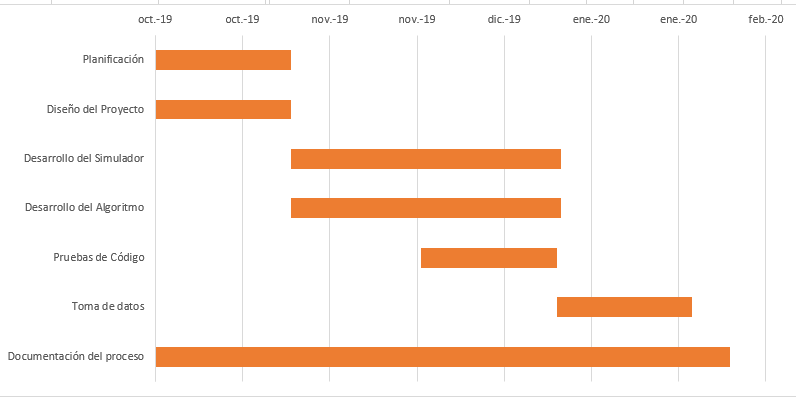
\includegraphics[width=0.6\textwidth]{figuras/gant1.png}   
\caption{Diagrama de Gantt de la planificación inical del proyecto}
\label{fig:gant1}
\end{figure}

Esta planificación inicial fue demasiado ambiciosa, sin tener en consideración la situación y la disponibilidad de recursos durante ese periodo planificado, lo que desembocó en la imposibilidad de cumplir esta planificación y tener que replantear toda la planificación.

\subsection{Planificación final}

Una vez que la planificación inicial del proyecto fue totalmente inviable, fue necesario restablecer la planificación del proyecto. La planificación final ha sido más realista, salvando las distancias con las demoras sufridas a raiz de acontecimientos de gran importancia en la vida cotidiana.

El diagrama de la planificación final es el diagrama de la figura \ref{fig:gant2}.

\begin{figure}[tb]
\centering
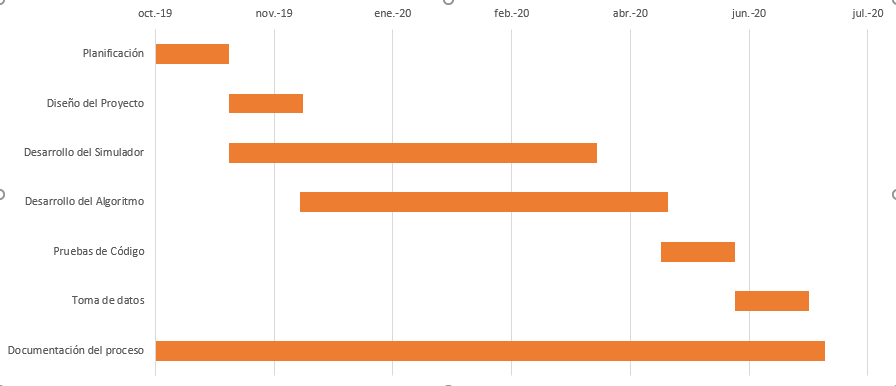
\includegraphics[width=0.6\textwidth]{figuras/gant2.png}   
\caption{Diagrama de Gantt de la planificación final del proyecto}
\label{fig:gant2}
\end{figure}

\section{Presupuesto}

Si bien no había una planificación sobre presupuesto a gastar ya que, al ser un proyecto de programación, no había previsión de realizar gastos económicos, algunos gastos económicos si que hubo.

\subsection{Material}
Al principio, no había ningún tipo de planteamiento de hacer gasto económico para este proyecto. Pero las necesidades a la que fue avanzando el proyecto cambiaron, y fue necesario disponer de los siguientes elementos:
\begin{itemize}
\item Una baraja francesa de póker. Si bien esto puede parecer algo básico e, incluso, innecesario, la adquisición de un kit de poker contribuyó bastante, sobre todo en las fases iniciales del proyecto, pues servía de ayuda visual para la codifcación del funcionamiento de una ronda de juego de Texas Hold'em. Debido a que fue utilizada principalmente en momentos de atasco de ideas, acabó convirtiéndose en una ayuda para la concentración.
\item Hold'em Excellence (English Edition). Debido a la dificultad de encontrar fuentes y bibliografía en torno a la fórmula de Chen, fue necesaria la adquisición del libro donde se definió por primera vez por Lou Krieger. \cite{krieger}.
\end{itemize}

Además de ello, los gastos a lo largo del proyecto en dosisfuertes de cafeína para poder aprovechar el tiempo al máximo al compaginar demasiadas cosas.

%\subsection{Personal}

%Si bien el proyecto no tenía intención de causar gasto personal, acabó generando mucho agotamiento y estrés, especialmente en las fechas de cumplimieto de la planificación (con mayor intensidad en la planificación inicial que en la final), que acabó provocando en privaciones largas de sueño.

\subsection{Resumen de costes}

\begin{longtable}[c]{ll|l|l|}
\hline
\rowcolor{lightgray}\multicolumn{1}{|l|}{\textbf{Elemento}} & \textbf{Cantidad} & \textbf{Coste unitario} & \textbf{Coste} \\ \hline
\multicolumn{1}{|l|}{\textit{Kit de Poker}} & 1 & 10 & 10 \\ \hline
\multicolumn{1}{|l|}{\textit{Hold'em Excelence (Kindle Edition)}} & 1 & 8,54 € & 8,54 € \\ \hline
 &  & \textbf{Total} & \textbf{18,54} \\ \cline{3-4} 

\end{longtable}

\chapter{Conclusiones}

Por último, se presentan las conclusiones a las que se ha llegado una vez se ha completado el proyecto.

\section{Conclusión}

Ahora que el proyecto ha finalizado, se pueden extraer varias conclusiones acerca de los resultados del proyecto, así como del proceso en sí. 

Lo primero, es analizar el cumplimiento de objetivos del proyecto.
Los 3 objetivos del proyecto (desarrollar un motor de juego capaz de ejecutar tanto un modo automático como uno con interacción humana, desarrollar un algoritmo de toma de decisiones capaz de tomar decisiones y la creación de un enlace funcional entre ambos elementos) han sido cumplidos, como se ha podido demostrar a lo largo de este documento.

Si bien el objetivo está cumplido, se considera que el objetivo de desarrollo del algoritmo de toma de decisiones no ha sido desarrollado hasta su máximo potencial, pues los datos obtenidos arrojan que parte del diseño y planteamiento iniciales no son adecuados para obtener un funcionamiento y rendimiento óptimo. 
La eficiencia del algoritmo es algo que necesita ser probado, ajustado y replanteado con mucha más profundidad, pues con los factores actuales, no termina de ser óptimo (al obtener un beneficio medio de  $-0,19957213\pm1,06969216$$\frac{bb}{partida}$, la tendencia es perder dinero, por lo que no es un resultado adecuado).

Para intentar determinar una de las posibles causas de este rendimiento, se introdujo un cambio que intentaba eliminar parte de la aleatoriedad del algoritmo, lo cual mejoró contra uno de los patrones, mientras que el resto de los patrones o empeoraba parcialmente su resultado o no había cambios significativos.
Debido a las limitaciones físicas para la toma de datos por los enormes tiempos de ejecución, en concreto del cálculo del potencial, las tomas de mediciones se alargaban durante varias horas solo para obtener 300 datos, no se pudo tomar la cantidad de datos deseados en un principio.

Por esto mismo, el muestreo de datos es limitado, siendo insuficiente para contrastar hipótesis sobre cuál o cuáles pueden ser los fallos en el diseño. Como segunda conclusión, se tendría que es necesario tomar más medidas, y más variadas (alterando valores y variables) con el fin de intentar detectar los errores.

Otra de las conclusiones que se sacan es la complejidad que esconde el proyecto. En las fases iniciales del proyecto no se tenía consciencia de lo compleo que podía llegar a resultar el análisis estadístico del póker y el diseño de un algoritmo de toma de decisiones. También se menospreció la complejidad y la dificultad que planteaba diseñar un simulador de juego funcional desde 0, que resultó ser bastante mayor de lo considerado en el planteamiento del diseño. 

Si bien el sentimiento con el que se acaba este proyecto es de satisfacción por haber cumplido los objetivos del proyecto, tiene un regusto agridulce por el resquemor de no haber sido capaz de lograr optimizar el algoritmo.

En el siguiente apartado, se dejan unos planteamientos futuros para este proyecto, futuras mejoras o posibles cambios de paradigma que puedan, o no, resultar en una mejora del proyecto.

\section{Desarrollos futuros}

Hay varios posibles caminos de acción para el futuro de este proyecto. Algunos de los posibles planteamientos para un desarrollo futuro son los siguientes.

\subsection{Corrección y perfeccionamiento del algoritmo}

El desarrollo más evidente. Dado que es la parte pendiente de este proyecto, el punto inmediato para un posible desarrollo sería proseguir desde este punto para mejorar los datos que ya se tienen. Ejecutar más pruebas para obtener más datos y contrastar la eficiencia del algoritmo actual, plantear los factores que puedan corregirse del diseño del algoritmo, mejorar el rendimiento de ejecución del algoritmo, modelar más tipos de adversarios, cambiar los modelados ya existentes, así como las correcciones del algoritmo actual... Son muchos los caminos de investigación y desarrollo los que se pueden tomar en este punto en pos de perfeccionar el algoritmo.

También sería interesante modelar a un patrón cambiante, e ir viendo como el algoritmo varía sus acciones en función de lo que estiime más cercano a sus acciones de ese momento.

Por otro lado, jugar con los datos filtrados por combinaMazoPot podría ser útil para intentar perfilar más el rango de acción. Actualmente es la media aritmética de $P_r$. ¿Qué pasaría si fuese el 75\% del valor máximo? ¿Cómo afectaría al rendimiento este cambio? ¿Cuánta precisión se pierde a cambio?

\subsection{Alternativas al diseño del algoritmo}

El algoritmo se ha diseñado desde el punto de vista del juego explotador basado en la estadística, intentando valorar las jugadas y posibles jugadas más probables e intentar leer las acciones del adversario para intentar sacar el máximo beneficio. Pero no es la única manera en la que se puede desarrollar el algoritmo.

Se puede plantear también un diseño en otras arquitecturas como las redes neuronales, por ejemplo. Podría ser interesante plantear un desarrollo del algoritmo en otra arquitectura, y comparar el rendimiento de ambos. Se podría llegar a obtener un algoritmo que no solamente tenga un resultado más eficiente, sino que también un rendimiento más alto.

\subsection{Modelado de jugadores adicionales}

El funcionamiento del simulador y el algoritmo se han centrado en la modalida HUNLdel Texas Hold'em, pero sería muy interesante el salirse del HUNL y codifcar otros jugadores. Esto supondría varías ideas y planteamientos sobre los que habría que razonar y plantear con seriedad, como, por ejemplo, cómo se modelaría más de un jugador,  cómo afectaría el modelado de cada jugador al algoritmo, cómo influiría el posicionamiento con respecto al \textit{dealer} al algoritmo, qué baremos cambiarían, cómo se modificarían las probabilidades y la estadísrica en función del número de jugadores totales, cómo se modificaría el modelado de los adversarios en el Flop, influiría el Ante en la toma de decisiones en caso de que haya más de dos jugadores,  se podrían hacer las abstracciones que se hacen, se tendrían que hacer nuevas abstracciones, etc...

\subsection{Mejora gráfica del simulador}

Esta es una de las posibles ideas para seguir adelante.El motor de juego esta programado como una aplicación de consola, sin ningún tipo de elemento gráfico que no sea una combinación de símbolos. Diseñar una nueva versión del simulador de juego, como una aplicación de ventana, programar de una forma mucho más visual y que permita leer con más facilidad toda la información que se calcula para el funcionamiento del simulador.


Estas serían algunas de las ideas que se plantean como posibles desarrollos futuros., Si bien no estricos, cualquier otro tema relacionado con el proyecto y no se hayan considerado sería interesante desarrollarlos también.

%\chapter{Cómo escribir en Latex}

\section{Citas}

%las referencias a artículos se ponen con \cite, 
%las referencias a imágenes \ref, 
%y las referencias a ecuaciones \eqref


.Esto es un ejemplo de cita de un artículo \cite{chen}


\section{Listas}

%itemize es una lista. Cada término lleva delante un \item
Ejemplo de lista de puntos:
\begin{itemize}
\item Ejemplo1.
\item Ejemplo2.
\end{itemize} 

Y lista numerada:
\begin{enumerate}
\item Elemento 1
\item Elemento 2
\end{enumerate}

\section{Tablas}

Ejemplo de tabla. Como se aprecia en la tabla \ref{tab:table_example}...
\begin{table}[tb]
\caption{Ejemplo de tabla}
\label{tab:table_example}
\begin{center}
\begin{tabular}{|c||c|c|}
\hline
One & Two & Three\\
\hline
F1A & F1B & F1C\\
F2A & F2B & F2C\\
\hline
\end{tabular}
\end{center}
\end{table}

\section{Referencia a una sección}
\label{sec:refsec}

Ejemplo de referencia a la sección \ref{sec:refsec}

\section{Texto}

Testo en \textbf{negrita} y \textit{cursiva}.

\section{Figuras}


\begin{longtable}[c]{|c|c|c|c|}
\end{longtable}

Ejemplo de referencia a figura (figura \ref{fig:logo_upm}). Es importante que todas las figuras que aparezcan estén referenciadas, así como las tablas. En general las figuras se colocarán al principio o al final de cada página ([tb] en latex), a no ser que por alguna necesidad se deban colocar en una posición exacta ([h]).

%caption es el pie de foto, y label es el nombre que se da a la imagen para referenciarla después. label no puede llevar acentos y no se muestra de cara al documento final (es sólo interno).
\begin{figure}[tb]
\centering

\includegraphics[width=0.45\textwidth]{figuras/Logo_UPM.jpg}   
\caption{Logotipo de la UPM}
\label{fig:logo_upm}
\end{figure}
\appendix

\chapter{Anexo A: Fundamentos de probabilidad}
\label{ch:AxA}

\section{Eventos y Probabilidad}

En el apartado \ref{sec:bayes}, se ha mencionado la probabilidad de que un evento ocurra, que es el número de casos posibles dividido entre el número de casos posibles. Una de las cosas importantes a tener en cuenta son los eventos cuando aparecen varios simultáneamente.
Hay que distinguir entre:
\begin{itemize}
\item Eventos excluyentes: son eventos que no pueden ocurrir simultáneamente. Por ejemplo, “La carta es de Picas” (P=1/4) y “La carta es de Corazones” (P=1/4) son eventos que no pueden ocurrir simultáneamente.
\item Eventos no excluyentes: son eventos que pueden ocurrir simultáneamente. Aquí tenemos que clasificar estos eventos por la relación que tienen entre ellos.
\begin{itemize}
\item Eventos independientes: Son eventos que no tienen efecto uno en el otro. Por ejemplo, “Una carta es del palo de diamantes” (P=1/4) y “una carta es un nueve” (P=1/13) son dos eventos que pueden ocurrir simultáneamente. 
\item Eventos dependientes: Son eventos que si influyen uno en el otro. Aquí también podemos considerar la probabilidad condicional de A teniendo B, que es la probabilidad de que, si ocurre B, A también ocurriera. 
\end{itemize} 
\end{itemize} 

La probabilidad de que ocurran ambos eventos dependientes es igual a la probabilidad de A multiplicado por la probabilidad condicional de B teniendo A, mientras que si los eventos son independientes si la probabilidad condicional de A teniendo B es igual a la probabilidad de A.
La nomenclatura a usar es la siguiente:
$p(A \cap B) \equiv$ Probabilidad de que ocurran A y B. Es decir, probabilidad de A y B.
$p(A \cup B) \equiv$ Probabilidad de que ocurran A o B. Es decir, probabilidad de A o B. 
p(A | B) $\equiv$ Probabilidad condicional de que ocurra A habiendo ocurrido B. Es decir, probabilidad de A teniendo B.
Y aquí tenemos algunas fórmulas sobre estas probabilidades:
\[
p(A \cup B) = p(A) + p(B) – p(A \cap B)
\]
\[
p(A\cap B) = p(A)*p(B | A)
\]
Teniendo en cuenta que los eventos excluyentes no pueden ocurrir simultáneamente ($p(A \cap B)_{excluyentes} = 0)$, podemos simplificar la primera fórmula para los eventos excluyentes:
$p(A \cup B)_{excluyentes} = p(A) + p(B)$
Tal y como hemos comentado antes, para eventos independientes, la probabilidad del evento B teniendo A es igual a la probabilidad de B, por lo que podemos simplificar la segunda ecuación:
$p(A \cap B)_{independientes} = p(A)*p(B)$
Mientras que para eventos dependientes es:
Además de estas fórmulas, podemos utilizar las siguientes propiedades de los eventos:
\[
0 \leq p(A) \leq 1\text{(para cualquier A)}
\]
\[
p(C) = 1
\]
\[
p(I) = 0
\]
\[
p(A) + p (\tilde{A}) = 1\rightarrow p (\tilde{A}) = 1 - p(A)
\]

Siendo:
$p(\tilde{A}) \equiv$ Probabilidad de que A no ocurra.
C $\equiv$ Evento verdadero
I $\equiv$ Evento imposible


\section{Distribuciones y Varianza}

Una vez tenemos las bases de la probabilidad de un evento o de eventos controlados, es necesario ampliar esta información para considerar diferentes probabilidades simultáneamente, pudiendo englobar los posibles resultados y sus respectivas probabilidades de un evento como una distribución de probabilidad.
Para el estudio del Texas Hold’em, esta distribución es un elemento que nos ayuda a intentar estimar las posibles manos que puedan tener los oponentes. Si bien al comienzo de la partida, la distribución de probabilidades de cada jugador es idéntica, a medida que avanzan las fases, se van incluyendo nuevos factores a tener en cuenta que permite estimar esa probabilidad de otra manera (tales como las cartas en la mesa, las cartas en nuestra mano, las apuestas…).

Cuando una distribución de probabilidad X tiene valores numéricos asociados a cada uno de los posibles resultados, dichas distribuciones de probabilidad tienen dos valores característicos que, en conjunto, describen la mayor parte de las distribuciones: valor esperado ($<X>$) y varianza ($V_X$).
Para una distribución de probabilidad X, con n posibles resultados de valor $x_i$ y cada uno con una probabilidad $p_i$, el valor esperado $<X>$ es: 
\[
<X> =\sum_{i=1}^ n p_ix_i
\]
La varianza, por su parte, es una medida de la desviación de los resultados de lo esperado en una distribución. Este valor siempre es positivo


Para una distribución de probabilidad X, con n posibles resultados de valor $x_i$ y cada uno con una probabilidad $p_i$, la varianza $V_x$ es: 
\[
V_x= \sum_{i=1}^ n p_i(x_i - <X>)^2
\]
La varianza nos ayuda para poder valorar las ganancias, pues una estrategia arriesgada y agresiva tendrá una varianza mucho mayor a una estrategia segura y pasiva, ya que los resultados de las apuestas estarán mucho más alejados de la media (ya que las ganancias serán mayores, pero las cantidades apostadas perdidas también lo serán). 
Teniendo en cuenta que el valor de la varianza es un valor resultado de un cuadrado, no siempre es fácil comparar dos eventos (y, mucho menos, valor esperado con varianza). Para eso existe la desviación ($\sigma$), que es la raíz cuadrada de la varianza.
\[
	\sigma =\sqrt{V}  \rightarrow \sigma^2= V
\]
A pesar de esto, la varianza y la desviación solo sirven como valor decisivo en caso de tener que estudiar el riesgo de apostar, para el resto de casos serán un valor meramente descriptivo.


\chapter{Anexo B: Manual de uso}
\label{ch:anexoc}

El objetivo de este apéndice es servir de guía para la ejecución del software diseñado, mostrar cómo es una partida del modo Jugador vs Máquina y mostrar los pasos a seguir para poner en marcha ambos modos.

Si bien el diseño del software está pensado para que resulte bastante intuitivo, se añade esta información para aclarar cualquier posible duda.


\section{Inicialización del algoritmo}

El primer paso es la inicialización del algoritmo necesaria para ejecutar los modos de juego \footnote{Solamente para los modos de juego en los que intervenga el algoritmo. Se puede ejecutar el modo Patrón vs Patrón sin necesidad de hacer este paso.}. Para ello, es necesario ejecutar un compilador de lenguaje R (el propio compilador de R instalado con la instalación de R en el equipo o otros más enfocados a la programación como RStudio) y cambiar el directorio de trabajo al directorio en que se encuentren todos los scripts del algoritmo. Tras esto, es necesario inicializar el sistema REST API. Para ello, tal y como se comentó en el apartado \ref{sec:APIrest}, se ejecutan los comandos necesarios:

\begin{verbatim}
source("inicializa.R")
inicializa()
r<-plumb("plumber.R")
r$run(port=8000).
\end{verbatim}

Cabe destacar que se utilizará el puerto 8000 para realizar la conexión con el API REST, y el motor de juego ha sido programado para leer desde ese puerto, por lo que si se decide cambiar el puerto, será necesario cambiar también el código del motor de juego.

Una vez arrancado el algoritmo, se puede arrancar el motor de juego, ejecutando el archivo \textit{Poker\_Simu.exe}, lo que abre una consola de comandos como la de la figura \ref{fig:C_ini}.

\begin{figure}[h]
\centering
\includegraphics[width=0.5\textwidth]{figuras/C_ini.png}   
\caption{Pantalla inicial de Poker\_Simu.exe}
\label{fig:C_ini}
\end{figure}

Tras esto, se elige la modalidad que se quiera jugar, escribiendo la letra J para el modo Jugador vs Máquina o M para el modo Máquina vs Máquina.

\section{Jugador Vs Máquina}

Una vez elegida esta modalidad, el propio juego te pedirá introducir la cantidad de dinero inicial para los jugadores y el valor de la Ciega Grande, tal como se muestra en la imagen \ref{fig:C_ji}.

\begin{figure}[h]
\centering
\includegraphics[width=0.5\textwidth]{figuras/C_ji.png}   
\caption{Pantalla inicial de Poker\_Simu.exe en el modo Jugador vs Máquina.}
\label{fig:C_ji}
\end{figure}

Una vez introducidos, se comenzará la partida, mostrando la mesa disponible para el jugador. Es decir, mostrará las cartas de la mano del jugador. Tras esto, comenzará el juego. Cada vez que sea el turno del jugador, siguiendo el flujo de juego. Este proceso se irá repitiendo hasta que uno pase o ambos vean la apuesta.
Una vez que se pase al preflop, mostrará las cartas de la mesa, tal y como aparece en la imagen \ref{fig:C_j2}.

\begin{figure}[h]
\centering
\includegraphics[width=0.5\textwidth]{figuras/C_j2.png}   
\caption{Flop en el modo Jugador vs Máquina.}
\label{fig:C_j2}
\end{figure}


\begin{figure}[h]
\centering
\includegraphics[width=0.5\textwidth]{figuras/C_JE.png}   
\caption{Subida de apuesta en el modo Jugador vs Máquina.}
\label{fig:C_JE}
\end{figure}

\begin{figure}[h]
\centering
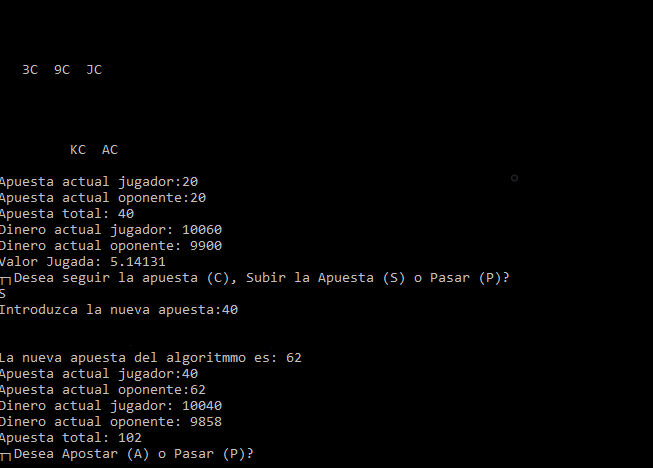
\includegraphics[width=0.5\textwidth]{figuras/C_J.png}   
\caption{Reacción del algoritmo ante una acción del jugador.}
\label{fig:C_J}
\end{figure}

En caso de hacer una subida, se pedirá que se introduzca la cantidad a subir, como aparece en \ref{fig:C_JE}. En caso de que el algoritmo tome una decisión, esta acción será mostrada y pedirá al jugador que tome una acción en caso de que sea necesario, tal como aparece en \ref{fig:C_J}.

\begin{figure}[h]
\centering
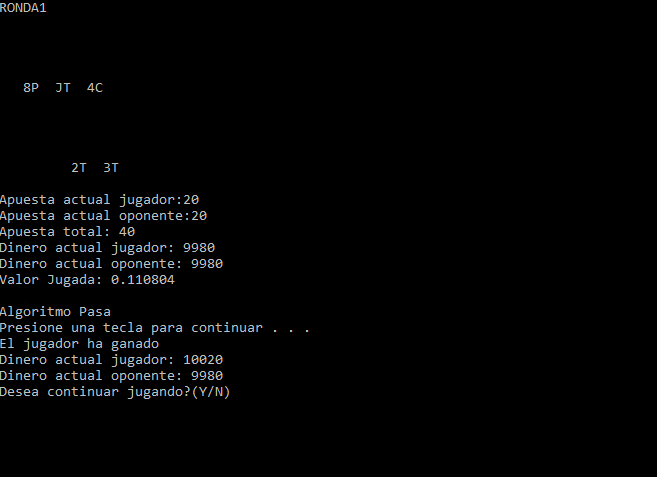
\includegraphics[width=0.5\textwidth]{figuras/C_jf.png}   
\caption{Fin de ronda.}
\label{fig:C_jf}
\end{figure}

Una vez que uno de los jugadores pase, o se llegue al showdown y se acabe la ronda de apuestas, se pedirá al jugador si quiere seguir jugando, a lo que tendrá que responder escribiendo Y en caso de que se quiera seguir jugando, o N en caso de querer acabar la partida. (Tal como se muestra en \ref{fig:C_jf}.)

\clearpage

\section{Máquina Vs Máquina}

En este apartado, se muestra cómo se desarrolla el juego en caso de haber elegido el modo Máquina vs Máquina. Una vez introducida la opción, se listarán los 3 patrones posibles (Maniaco, Roca y Calling Station), tras lo cual se pide al jugador introducir que modo dentro del modo Máquina vs Máquina. Tal como se muestra en la figura

\begin{figure}[h]
\centering
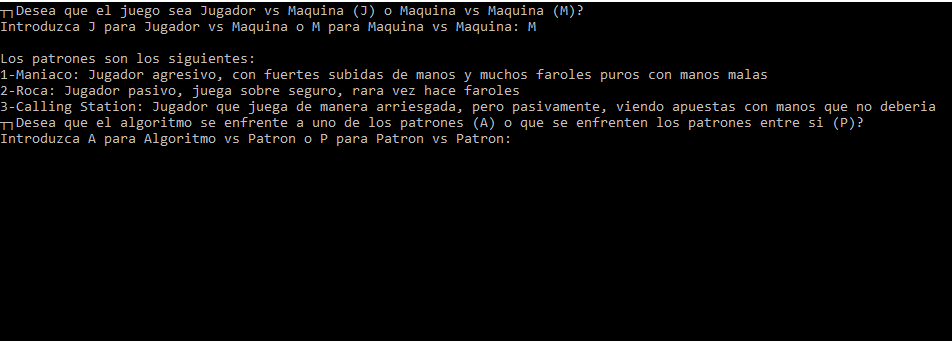
\includegraphics[width=0.5\textwidth]{figuras/C_M.png}   
\caption{Pantalla de inicio del modo Máquina vs Máquina.}
\label{fig:C_M}
\end{figure}

En caso de que se elija el modo Patrón vs Patrón, se mostrarán las tres combinaciones (Maniaco vs Roca, Roca vs Calling Station y Calling Station vs Maniaco) y después pide al jugador que introduzca la combinación de patrones que quiere que se enfrenten (como aparece en la imagen \ref{fig:C_MM}) . En caso de que se elija el modo Algoritmo vs Patrón, se pedirá al jugador que introduzca a cual de los 3 patrones desea que se enfrente al algoritmo (como se muestra en la imagen \ref{fig:C_MA}). Tras eso se pide al jugador que introduzca el dinero inicial de cada jugador, así como el valor de la Ciega Grande. Por último, se pide introducir el número de interacciones deseadas.

\begin{figure}[h]
\centering
\includegraphics[width=0.5\textwidth]{figuras/C_MM.png}   
\caption{Pantalla de inicio del modo Patrón vs Patrón.}
\label{fig:C_MM}
\end{figure}

\begin{figure}[h]
\centering
\includegraphics[width=0.5\textwidth]{figuras/C_MA.png}   
\caption{Pantalla de inicio del modo Algoritmo vs Patron..}
\label{fig:C_MA}
\end{figure}

Estas iteracciones se irán ejecutando sin necesidad de intervención por parte del jugador. Una vez se alcance una de las condiciones de fin de juego (se alcance el número de iteraciones o uno de los jugadores se quede sin dinero), finalizará el programa. El resultado de las iteraciones se almacenará en un fichero .txt, con un formato como el que se mostró \ref{fig:resultados}.

\backmatter
%Glosario, lista de símbolos, notas, etc.

%estilo de bibliografía: plana, alfa...
\bibliographystyle{plain}

%genera doble hoja en blanco
\cleardoublepage

%apartado de bibliografía
\addcontentsline{toc}{chapter}{Bibliografia}

%se incluye la bibliografía. Archivo de tipo .bib (bibtex)
\bibliography{bibliografia/bibliografia}

%fin del documento
\end{document}